%oifusdjffasd
\documentclass[12pt, oneside]{book}
\usepackage{geometry}           % to change size of margins
\geometry{tmargin=0.70in, bmargin=0.70in, lmargin=1.2in, rmargin = 1.2in}
%TODO feels a bit too full with these settings /William
\usepackage{amsthm}             % for all the theorem-like environments
\usepackage{tikz-cd}            % for commutative diagrams
\usetikzlibrary{math}           % for some stuff with tikz drawings
%\usepackage{newpxtext,newpxmath}   % font, but it causes a problem with \bigcup and all big operators
\usepackage{mathpazo}           % math font

\usepackage[hidelinks]{hyperref}% for hyperlinks
\usepackage{float}              % for the H position modifier for figures
\usepackage{threeparttable}     % for measuredfigure but I don't know why it's used
\usepackage{subcaption}         % for the subfigure environment
\usepackage{mathrsfs}           % for the nice letters for categories
\usepackage{mathtools}          % for coloneq (:=) and xRightarrow (\implies with writings over or under)
\usepackage{quiver}             % for commutative diagrams from q.uiver.app
\usepackage{epigraph}           % for epigraphs, the quotes at the beginning of sections
\usepackage{microtype}          % reduces the number of overfull/underfull boxes
\usepackage{pdfpages}           % to include other pdfs (for titlepage)
\usepackage{dsfont}				% special S for sphere spectrum
\usepackage{bbding}				%For the plane symbol
\usepackage{ stmaryrd }			% to use \mapsfrom
\usepackage{fourier}				%for the danger symbol
\usepackage[mathscr]{euscript}	%for cooler curly letters for cats, especially 'S'
%\usepackage[all,cmtip]{xy}     % don't know what it's for
%\usepackage{upgreek}           % don't know what it's for
%\usepackage[normalem]{ulem}    % don't know what it's for
%\usepackage{graphics}          % don't know what it's for
%\usepackage{graphicx}          % don't know what it's for
%\usepackage{blindtext}         % don't know what it's for
%\usepackage{caption}           % don't know what it's for
%\usepackage{amsmath}           % don't know what it's for
%\usepackage{amssymb}           % don't know what it's for
%\usepackage{calrsfs}           % don't know what it's for
%\usepackage{wasysym}           % don't know what it's for
%\usepackage{verbatim}          % don't know what it's for
%\usepackage{bbm}               % don't know what it's for
%\usepackage{color}             % don't know what it's for
%\usepackage{xcolor}            % don't know what it's for

%I don't think having the "back to" sections /William
%TODO decide how to indicate interior, in some points there's the dot and in other int /William
%I think we never comment on bordism or CObordism, maybe add a comment somewhere /William

\makeatletter %adjusting the color of the entire document
\newcommand{\globalcolor}[1]{%
  \color{#1}\global\let\default@color\current@color
}
\makeatother

\AtBeginDocument{\globalcolor{magenta!10!black}}

\newcommand{\updateinfo}[1][\today]{\par\vfill\hfill{\scriptsize\color{red}Last updated on #1}}

\newcommand{\extra}{\texorpdfstring{\textmd{\Plane}\;\,}{plane}}

% \ensuremath to be able to write \R instead of $\R$
\newcommand{\R}{\ensuremath{\mathbb{R}} }
\renewcommand{\H}{\ensuremath{\mathbb{H}} }
\renewcommand{\P}{\ensuremath{\mathbb{P}} }
\newcommand{\C}{\ensuremath{\mathbb{C}} }
\newcommand{\Z}{\ensuremath{\mathbb{Z}} }
\newcommand{\N}{\ensuremath{\mathbb{N}} }
\newcommand{\Q}{\ensuremath{\mathbb{Q}} }
\newcommand{\E}{\ensuremath{\mathbb{E}} }
\newcommand{\F}{\ensuremath{\mathbb{F}} }
\newcommand{\K}{\ensuremath{\mathbb{K}} }
\newcommand{\T}{\ensuremath{\mathcal{T}} }
\newcommand{\A}{\ensuremath{\mathcal{A}} }
\newcommand{\Zf}{\ensuremath{\mathcal{Z}} }
\newcommand{\bat}{\ensuremath{\mathscr{B}} }
\newcommand{\cat}{\ensuremath{\mathscr{C}} }
\newcommand{\dat}{\ensuremath{\mathscr{D}} }
\newcommand{\eat}{\ensuremath{\mathscr{E}} }
\newcommand{\sat}{\ensuremath{\mathscr{S}} }
\newcommand{\unit}{\ensuremath{\mathbb{1}} }
\newcommand{\g}{\ensuremath{\mathfrak{g}} }
\newcommand{\gl}{\ensuremath{\mathfrak{gl}} }
\renewcommand{\sl}{\ensuremath{\mathfrak{sl}} }

\newcommand{\bbar}[1]{\overline{#1}} % a bar that covers the entire expression
\newcommand{\de}{\partial}
\newcommand{\acts}{\,\rotatebox[origin=c]{-90}{$\circlearrowright$}\,}

\DeclareMathOperator{\grad}{grad}
\DeclareMathOperator{\Hess}{Hess}
\DeclareMathOperator{\Bord}{Bord}
\DeclareMathOperator{\ind}{ind}
\DeclareMathOperator{\im}{im}
\DeclareMathOperator{\orient}{or}
\DeclareMathOperator{\fr}{fr}
\DeclareMathOperator{\id}{id}
\DeclareMathOperator{\tr}{tr}
\DeclareMathOperator{\sign}{sign}
\DeclareMathOperator{\fd}{fd}

% CATEGORY STUFF
\DeclareMathOperator{\ob}{ob}
\DeclareMathOperator{\Hom}{Hom}
\DeclareMathOperator{\End}{End}
\DeclareMathOperator{\Alg}{Alg}
\DeclareMathOperator{\Set}{Set}
\DeclareMathOperator{\Top}{Top}
\DeclareMathOperator{\Vect}{Vect}
\DeclareMathOperator{\Ab}{Ab}
\DeclareMathOperator{\Mon}{Mon}
\DeclareMathOperator{\Grp}{Grp}
\DeclareMathOperator{\AbGrp}{AbGrp}
\DeclareMathOperator{\Ring}{Ring}
\DeclareMathOperator{\Cat}{Cat}
\DeclareMathOperator{\Gpd}{Gpd}
\DeclareMathOperator{\SymmMonCat}{SymmMonCat}
\DeclareMathOperator{\nCob}{nCob}
\DeclareMathOperator{\Bordn}{Bord_{n,n-1}}
\DeclareMathOperator{\Bordnor}{Bord^{or}_{n,n-1}}
\DeclareMathOperator{\TFT}{TFT}
\DeclareMathOperator{\Mat}{Mat}
\DeclareMathOperator{\cFrob}{cFrob}
\DeclareMathOperator{\Diff}{Diff}
\DeclareMathOperator{\Conf}{Conf}
\DeclareMathOperator{\uConf}{uConf}
\DeclareMathOperator{\Braid}{Braid}
\DeclareMathOperator{\Tang}{Tang}
\DeclareMathOperator{\Mod}{Mod}
\DeclareMathOperator{\Aut}{Aut}
\DeclareMathOperator{\Fun}{Fun}
\DeclareMathOperator{\Link}{Link}
\DeclareMathOperator{\Rep}{Rep}
\DeclareMathOperator{\Lie}{Lie}
\DeclareMathOperator{\Der}{Der}
\DeclareMathOperator{\Disk}{Disk}
\DeclareMathOperator{\SmoothMfld}{SmoothMfld}


% ready made Torus drawing
\tikzset{
  pics/torus/.style n args={3}{
    code = {
      \providecolor{pgffillcolor}{rgb}{1,1,1}
      \begin{scope}[
          yscale=cos(#3),
          outer torus/.style = {draw,line width/.expanded={\the\dimexpr2\pgflinewidth+#2*2},line join=round},
          inner torus/.style = {draw=pgffillcolor,line width={#2*2}}
        ]
        \draw[outer torus] circle(#1);\draw[inner torus] circle(#1);
        \draw[outer torus] (180:#1) arc (180:360:#1);\draw[inner torus,line cap=round] (180:#1) arc (180:360:#1);
      \end{scope}
    }
  }
}
% ``



\newtheorem{thm}{Theorem}[section]
\newtheorem{prop}[thm]{Proposition}
\newtheorem{lem}[thm]{Lemma}
\newtheorem{cor}[thm]{Corollary}
\newtheorem*{clm}{Claim}
\newtheorem*{fct}{Fact}
\theoremstyle{remark}
\newtheorem*{rem}{Remark}
\theoremstyle{definition}
\newtheorem{defn}[thm]{Definition}
\newtheorem*{conv}{Convention}
\newtheorem*{rmnd}{Reminder}
\newtheorem*{notat}{Notation}
\newtheorem{ex}[thm]{Example}

%-----> packages for integrating the exercsises 
\usepackage{enumitem}
\theoremstyle{definition}
\newtheorem{exercise}[thm]{Exercise}


\title{\textcolor{black}{Bordism \& Topological Field Theory}}
\author{\Large{\textit{\textcolor{black}{Claudia Scheimbauer}}}}
\date{\textcolor{black}{Wintersemester 2023}}


\begin{document}
%\nocite{abc} for the books/lectures notes/articles

% all the following is to make the titlepage, but in the book format it gets screwed up
% \begin{figure}[t]
%      \centering
%      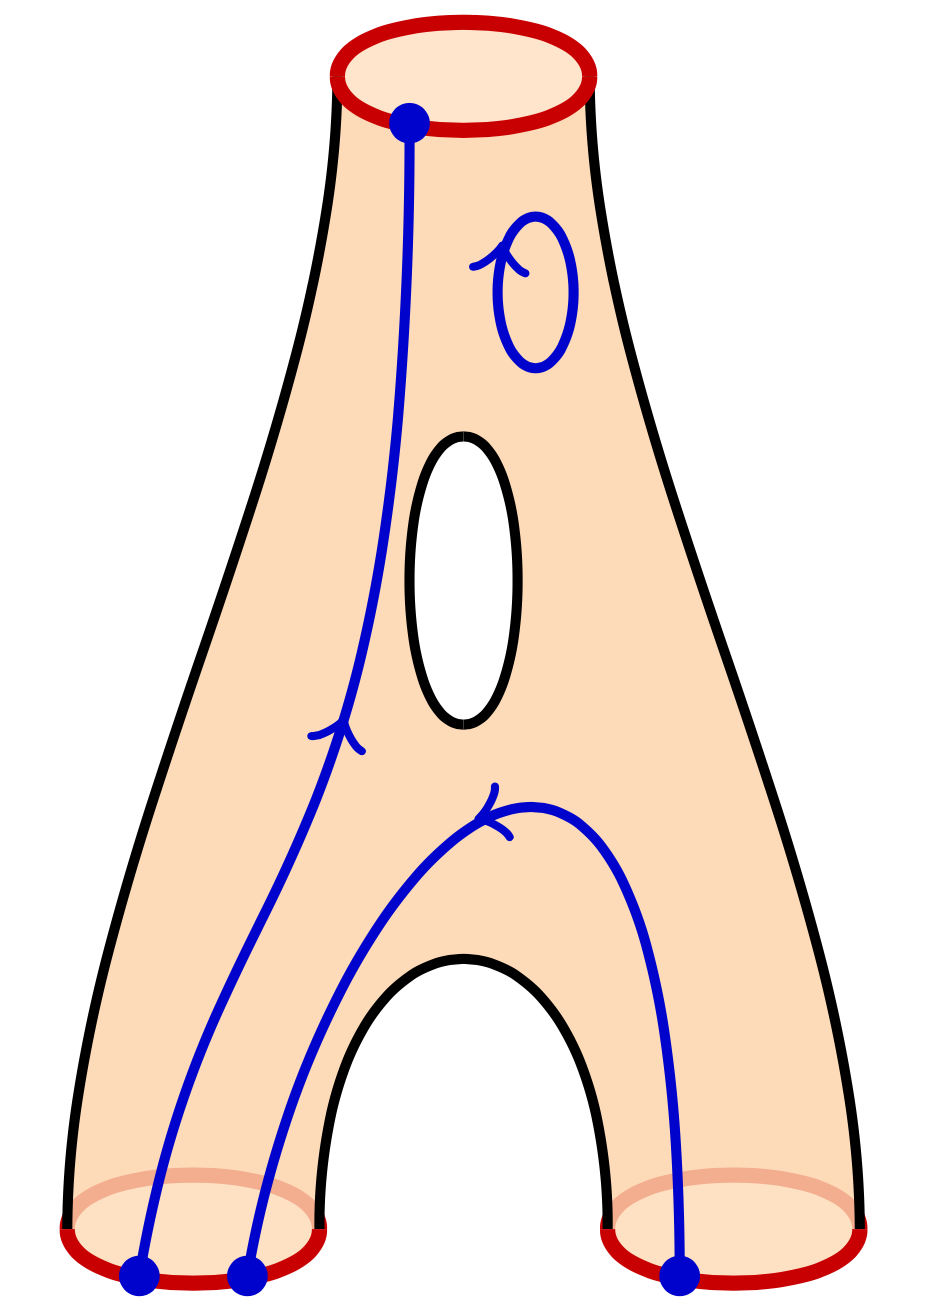
\includegraphics[width=9.50cm]{images/Lecture 1/cover.png}
%      \vspace{1mm}
%  \end{figure}
% \maketitle

% \thispagestyle{empty}

% \vspace{2mm}
% \begin{minipage}[t]{0.47\textwidth}
% 	 \textnormal{\large{\bf \textcolor{black}{Tutor:\\[2mm]}}}{\large \textcolor{black}{Anja \v{S}vraka}}
% \end{minipage}
% \hfill
% \begin{minipage}[t]{0.47\textwidth}\raggedleft
% 	 \textnormal{\large{\bf \textcolor{black}{Notes created by:\\[2mm]}}}
% 	 {\large \textcolor{black}{Luca Ipsale}}\\
%       {\large\textcolor{black}{William Luciani}}\\
%       {\large\textcolor{black}{Andrea Sittoni}}\\
%       {\large\textcolor{black}{Üzeyir Sa\c{c}{\i}kay}}\\
%       {\large\textcolor{black}{Jacob Skarby}}
% \end{minipage}

\pagenumbering{roman}
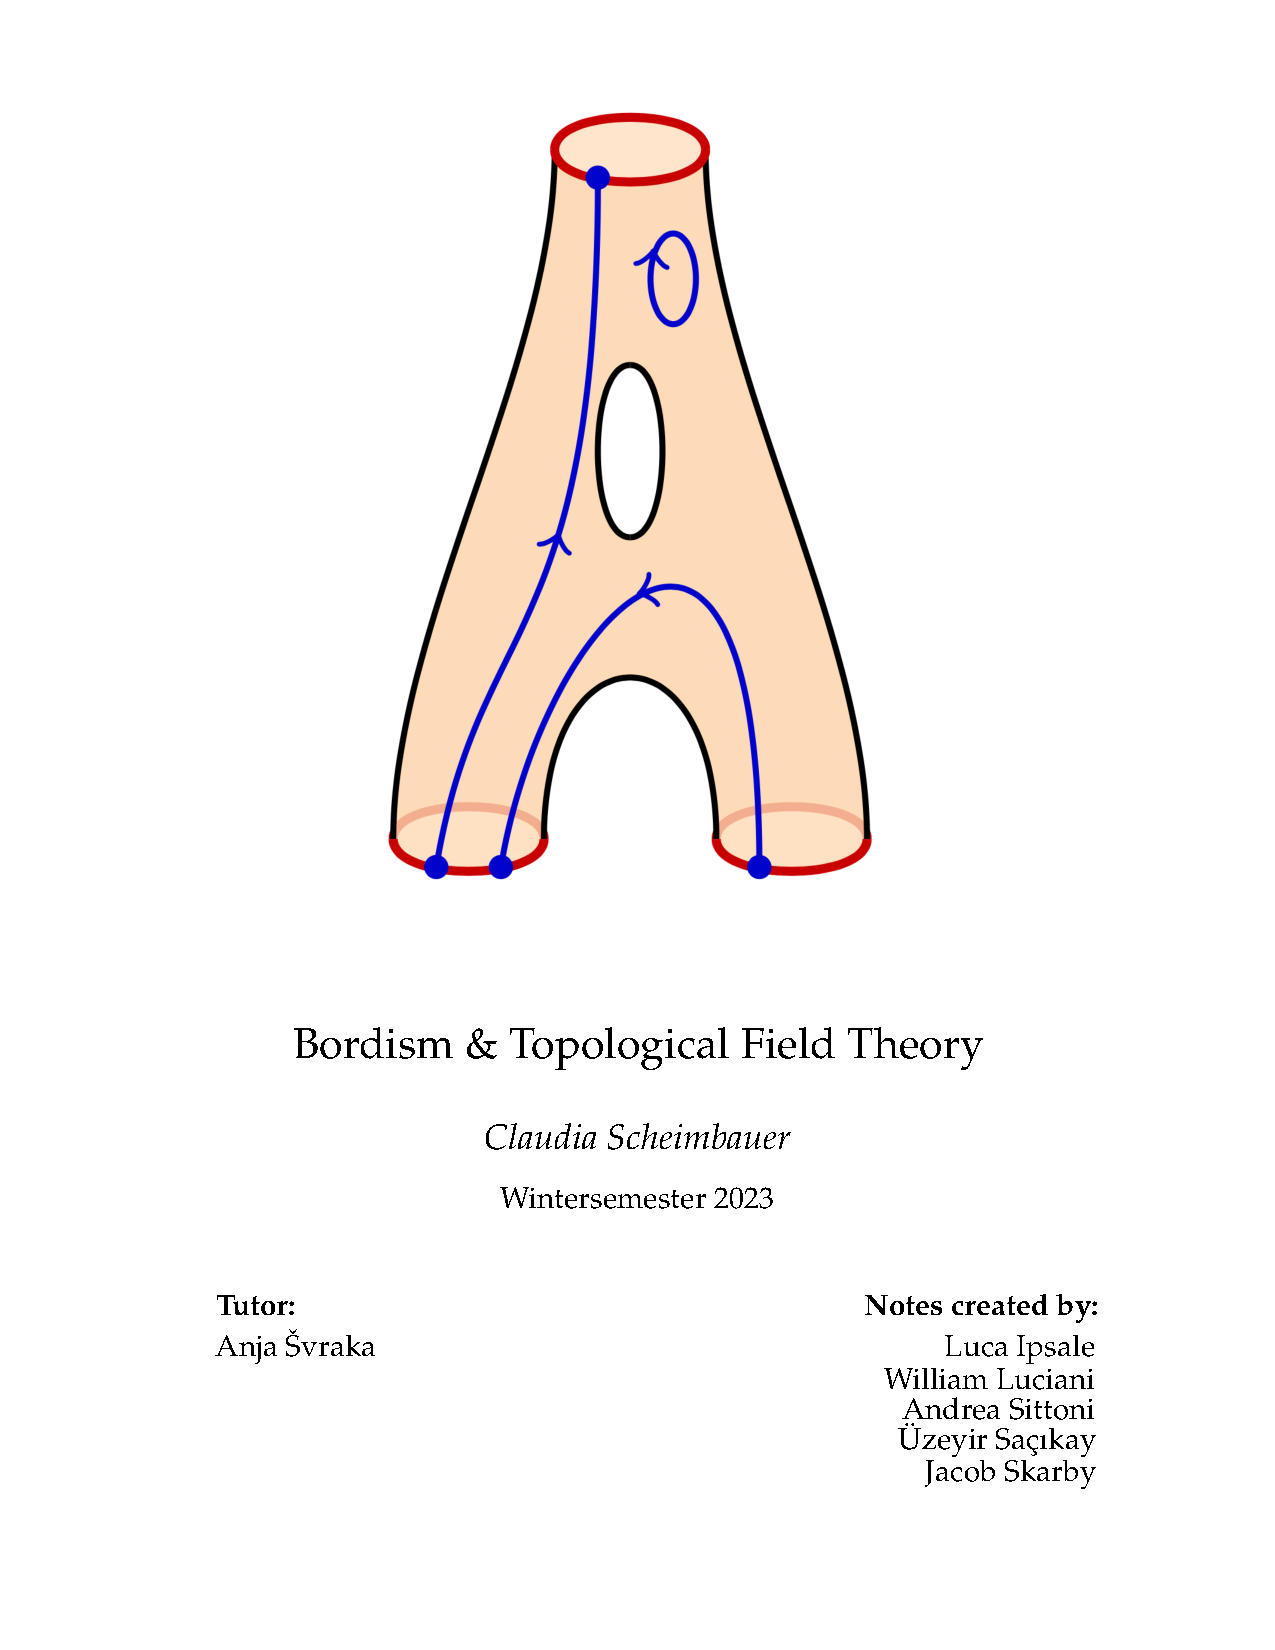
\includepdf{titlepage}

\clearpage
\thispagestyle{empty}
\cleardoublepage

\clearpage
\thispagestyle{empty}
\begin{flushright}
\null\vspace{\stretch{1}}
\textit{The mathematical facts worthy of being studied\\
are those which, by their analogy with other facts,\\
are capable of leading us to the knowledge of a mathematical law\\
just as experimental facts lead us to the knowledge of a physical law.\\
They reveal the kinship between other facts, long known,\\
but wrongly believed to be strangers to one another.\\
\hfill\break
$-$H. Poincaré}\\
\vspace{\stretch{2}}\null
\end{flushright}
\clearpage

\chapter*{\huge{\textcolor{black}{For the reader}}}
\hfill
\vspace{0.50cm}\\
These are the lecture notes of the course \textit{``Bordism and Topological Field Theory''} held by Prof.\hspace{1mm}Dr. Claudia Scheimbauer (\href{mailto:scheimbauer@ma.tum.de}{scheimbauer@ma.tum.de}) during the Wintersemester 2023/2024 at the \textit{Technische Universität München}. The tutorial sessions are held by Anja \v{S}vraka (\href{mailto:svr@ma.tum.de}{svr@ma.tum.de}).\hspace{1.5mm}The notes are typed by Luca Ipsale (\href{mailto:luca.ipsale@campus.lmu.de}{luca.ipsale@campus.lmu.de}), William Luciani (\href{mailto:w.luciani@campus.lmu.de}{w.luciani@campus.lmu.de}), Andrea Sittoni (\href{mailto:sittoniandrea@gmail.com}{sittoniandrea@gmail.com}) and Üzeyir Sa\c{c}{\i}kay (\href{mailto:uzeyirsacikay@gmail.com}{uzeyirsacikay@gmail.com}). Exercises are also implemented in the notes by Jacob Skarby (\href{mailto:jacob.skarby@tum.de}{jacob.skarby@tum.de}). If you find errors or if you have suggestions of any kind, please write us an e-mail.

\vspace{1cm}

{\LARGE \danger These notes have not been proofread by Prof. Scheimbauer, use at your own risk}.

\updateinfo
\thispagestyle{empty}



\clearpage
\thispagestyle{empty}
\cleardoublepage
\section*{Notational Conventions}
We use the symbol '\Plane' at the end of titles of sections, definitions or theorems that depart from the content of the lecture and deepen some aspect on a topic with an outlook towards research topics.

\begin{notat}
	Throughout these notes we will abuse notation indicating a collection with some structure on it just by writing down the collection, e.g. denoting a monoid $(M,\cdot)$ by $M$, a metric space $(X,d)$ by $X$ etc...
\end{notat}
\begin{notat}
	$n$-manifold and $n$-bordism mean respectively $n$ dimensional manifold and $n$ dimensional bordism.
\end{notat}
\begin{notat}
	We often denote equivalence classes just with a representative thereof. 
\end{notat}
\begin{notat}
We denote the category of spaces/$\infty$-groupoids both with $\mathscr{S}$, $\operatorname{Grpd}_\infty$ and with $\infty\operatorname{-Grpd}$. This is motivated by the homotopy hypothesis \ref{HomotopyHypothesis}.
\end{notat}
\begin{notat}
When there is no ambiguity, we denote $(\infty,1)$-categories as $\infty$-categories.
\end{notat}
\section*{Prerequisites}
The notes strive to be as self-contained as possible. We do assume however knowledge of linear algebra,
basic notions from analysis, e.g. $C^{\infty}$ differentiability, and basic notions of topology, e.g. 
paracompactness. Knowledge of algebraic topology is helpful but not necessary to understand the
most important parts.
\section*{Acknowledgements}
Apart from Prof. Scheimbauer's lectures and the cited references,
we often got inspiration from the nLab (\url{https://ncatlab.org/nlab/show/HomePage}) and from notes
on algebraic topology by Prof. Land (available on \url{https://www.mathematik.uni-muenchen.de/~gritscha/TOP1-23.php}).

\thispagestyle{empty}
\hfill
\vspace{0.50cm}
\textcolor{black}{\tableofcontents}


\newpage
\clearpage
\pagenumbering{arabic}



% -------------------------------------------------------------
% --------------------- LECTURE 1 23/10 -----------------------
% -------------------------------------------------------------

%TODO I would label and caption the figures so they can be referenced and they can appear wherever TeX thinks best /William

\chapter{Why should you care? An informal introduction}
%As the name suggests, this subject is two-sided: we have a physics part, namely Quantum Field Theory, and a mathematics part, more specifically topology and in particular (Co)Bordism. Let us explore the motivations and ideas behind these two subjects and how they come together. Do not worry if everything is not immediately clear, it will become so during the semester... hopefully. /// Andre: there is nothing wrong with this, just liked more the alternative I wrote down, feel free to change it back /AAndre
There are two ways one can approach topological field theories:
\begin{enumerate}
	\item As a way to make (some\footnote{Sadly, TFTs cannot axiomatize many quantum field theories that are particularly useful in physics, e.g. the quantum field theory behind the standard model.}) quantum field theories more mathematically rigorous
	\item As a way to refine bordism invariants, or, roughly, as a kind of homology for smooth manifolds of a certain dimension, instead of general topological spaces.
\end{enumerate}
We now sketch how the former might make sense.
\section{QFT}
\epigraph{Physics is very interesting:
There are many, many interesting theorems.
Unfortunately, there are no
definitions.}{David Kazhdan}
\noindent Start with a (smooth) manifold $M$ and, generally, some extra structure. For example:
\begin{itemize}
    \item $M^4=\R^4$ with a metric with signature $(+, +, +, -)$, so that we can distinguish a strictly spatial part and a temporal part $(\R^4=\R^3_{space}\times\R^1_{time})$. This is called \textit{Minkowski Spacetime} and is particularly important in QFT being the geometric foundation of Special Relativity,
    \item $M^3=\R^3$ with the Euclidean metric,
    \item $M^2$ with a conformal structure,
    \item $M^{11}$ as an ``Elliptic Fibration'', something which \textit{locally} looks like $\left(S^1\times S^1\right)\times \ something$. These things are useful in areas with high-sounding names such as ``M-Theory'' or, more generically, ``String Theory''.
\end{itemize}
However, in general, these manifolds must be thought of with other structures, like connections, bundles...\\
Now we can ``define'' a Quantum Field Theory on $M$ via a list of ingredients:
\begin{enumerate}
    \item \textbf{\textit{Fields}}. The \underbar{space} of fields $\mathcal{F}$, associated usually to a bundle $E\xrightarrow{p}M$, is defined as sections\footnote{A section of a bundle $E\xrightarrow{p}M$ is a map (in this context, smooth) $s:M\to E$ such that $p\circ s=id_M$.} of $E$ over $M$. In the case the bundle is trivial ($E\cong M\times X$), then $\mathcal{F}=\Gamma(M,E)=\text{Maps}(M\rightarrow X)$. But what mathematical object are we dealing with? What do we mean by ``space'' here? Is it a set, a topological space, a category, a scheme, a stack...?\\
    \begin{figure}[!ht]
        \centering
        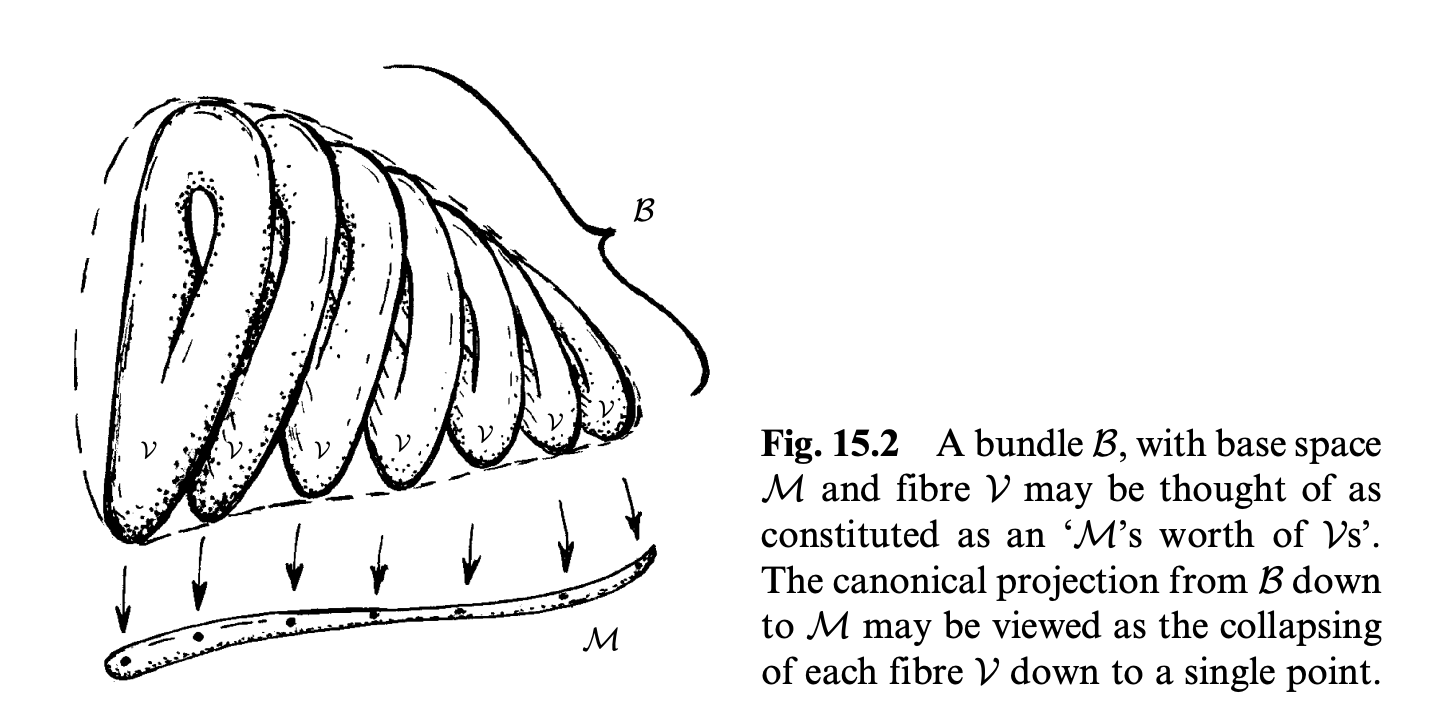
\includegraphics[width=8cm]{images/Lecture 1/penrose.png}
    \end{figure}
    %
    \item \textbf{\textit{Partition Function}}. We need a measure against which we can compute ``correlation functions'' of fields $\psi_1,\psi_2$ i.e. the ``likelihood of $\psi_1$ given $\psi_2$''. We thus define a Partition Function
    $$Z(M)=\int_{\psi\in\mathcal{F}}\ e^{iS(\psi)}\mathcal{D}\psi,$$
    with
    $$S(\psi)=\int_M \mathcal{L}(\psi),$$
    called the Action Functional. Generally $\mathcal{L}$ is a polynomial in the fields and it has derivatives. From the Partition Function one can obtain the correlation functions. Although physicists use this formula all the time, formally there is a problem: the measure $\mathcal{D}\psi$ is, in most cases, ill defined.
    \begin{figure}[!ht]
        \centering
        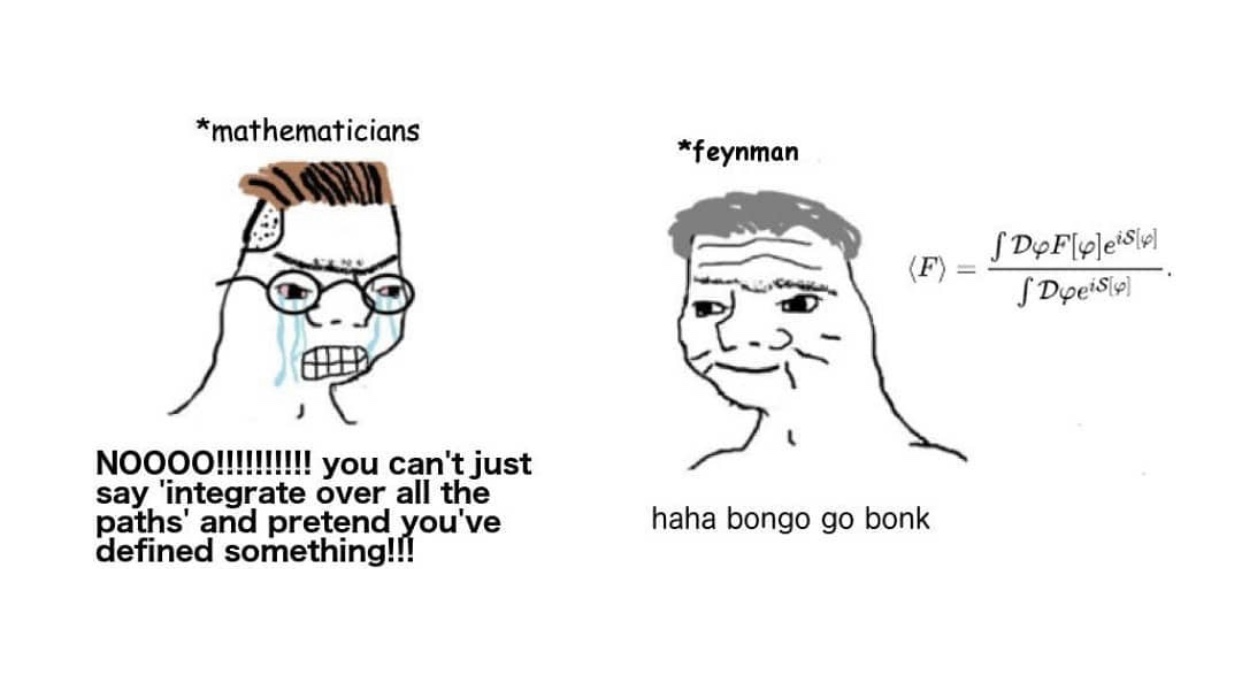
\includegraphics[width=9.2cm]{images/Lecture 1/feynman.png}
    \end{figure}
    %
    \item \textbf{\textit{Quantization}}. Often QFT arises from ``quantizing'' something classical. But what does this mean? And in what way does this thing behave when changing input?
\end{enumerate}
Physicists use all sorts of techniques (Feynman Diagrams, renormalization...) to make sense of undefined measures and divergences of all kinds emerging from calculations, dealing with things like $\infty-\infty$ or $\infty/\infty$ and obtaining finite and testable results.

\noindent This black box that physicists have (successfully) developed frustrates mathematicians because they do not understand why it works!
Therefore, axiomatizations have been developed exploiting new tools from geometry, algebra and topology to develop a formal and rigorous framework\footnote{More specifically to the path integral, see \cite[2.1]{Carqueville_2018} for an introduction on how topological field theories can be seen as a way to axiomatize some properties of the path integral as a tool to compute correlation functions.}.

\noindent The Partition Function $Z$ behaves well when ``smoothly'' changing the metric and is (in most cases) independent of most extra data of the manifold, so $Z(M)$ depends only on the smooth manifold and as such is purely topological!

\bigskip

If someone is into mathematics for the money or the prestige\footnote{If not already sufficiently clear, we explicitly state that this is a joke.}, the field of topological field theories is the one to specialize in:
 \begin{itemize}
    \item René Thom, the mathematician who laid the foundation of cobordism theory\footnote{Which is at the root of TFTs: TFTs can be seen as a refinement of his work.} in his PhD thesis, received the Fields Medal for this.
    % TODO is secondary here correct? What does it mean? Also, I would write Chern classes instead of Chern-Simons forms/William 
    \item Shiing-Shen Chern and Jim Simons discovered geometric invariants of 3-dimensional Riemannian manifolds called (classical) Chern-Simons invariants. They are a generalization of the total geodesic curvature, which is in turn a generalization of the curvature of a plane curve that $=0$ when the curve is a geodesic. Such invariants are the basic building blocks Witten used to define the earliest example we have of a TFT: 3d Chern-Simons theory\footnote{One can find more on this in \cite{freed2008remarks}}. Simons  then went on to found an incredibily successful hedge fund and became a billionaire. Chern continued to do groundbreaking work in differential geometry and topology; so much that some years ago the International Congress of Mathematicians named a prize after him: the \hyperlink{https://en.wikipedia.org/wiki/Chern_Medal}{Chern Medal}.
    \item Edward Witten received his Fields medal mainly because he found a link between 3d-TFTs, in particular Chern-Simons theory, and knot theory, in particular with the Jones polynomial. See \cite{Witten1989} for details.
\end{itemize} 
The Jones polynomial is a topological invariant of a knot, meaning that you can assign to each knot a Jones Polynomial in such a way that if two Knots have different polynomials, then they must be different.
\begin{center}
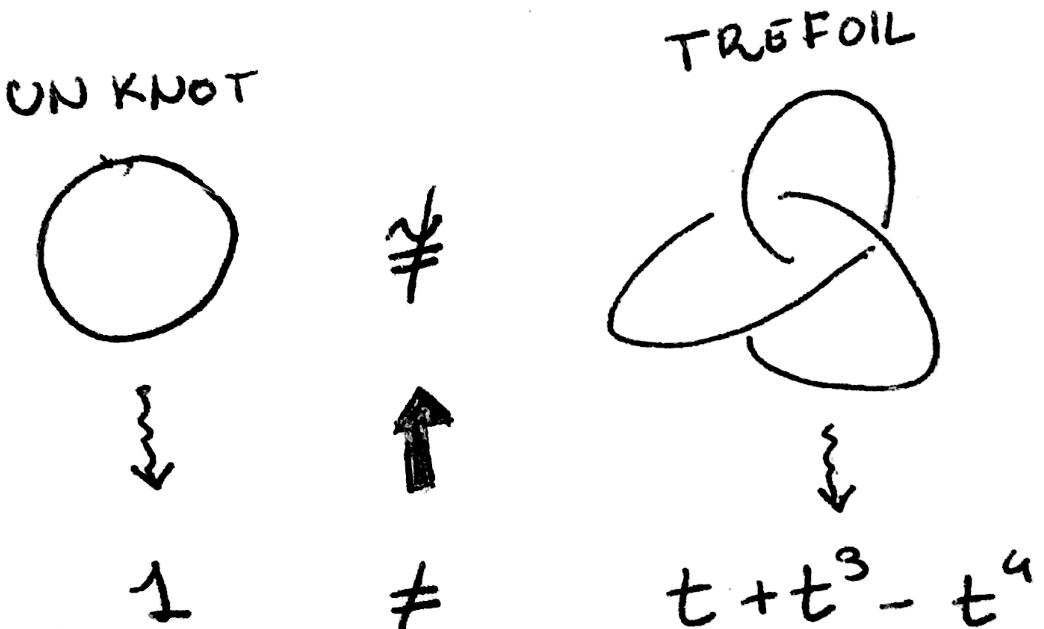
\includegraphics[width=5cm]{images/Lecture 1/Jones.jpg}
\end{center}
What the heck do TFTs and knots have in common?! There is actually a deep connection between the two.
When writing his paper, Witten drew several pictures like the following:
%The order of the images is compiled strangely
\begin{center}
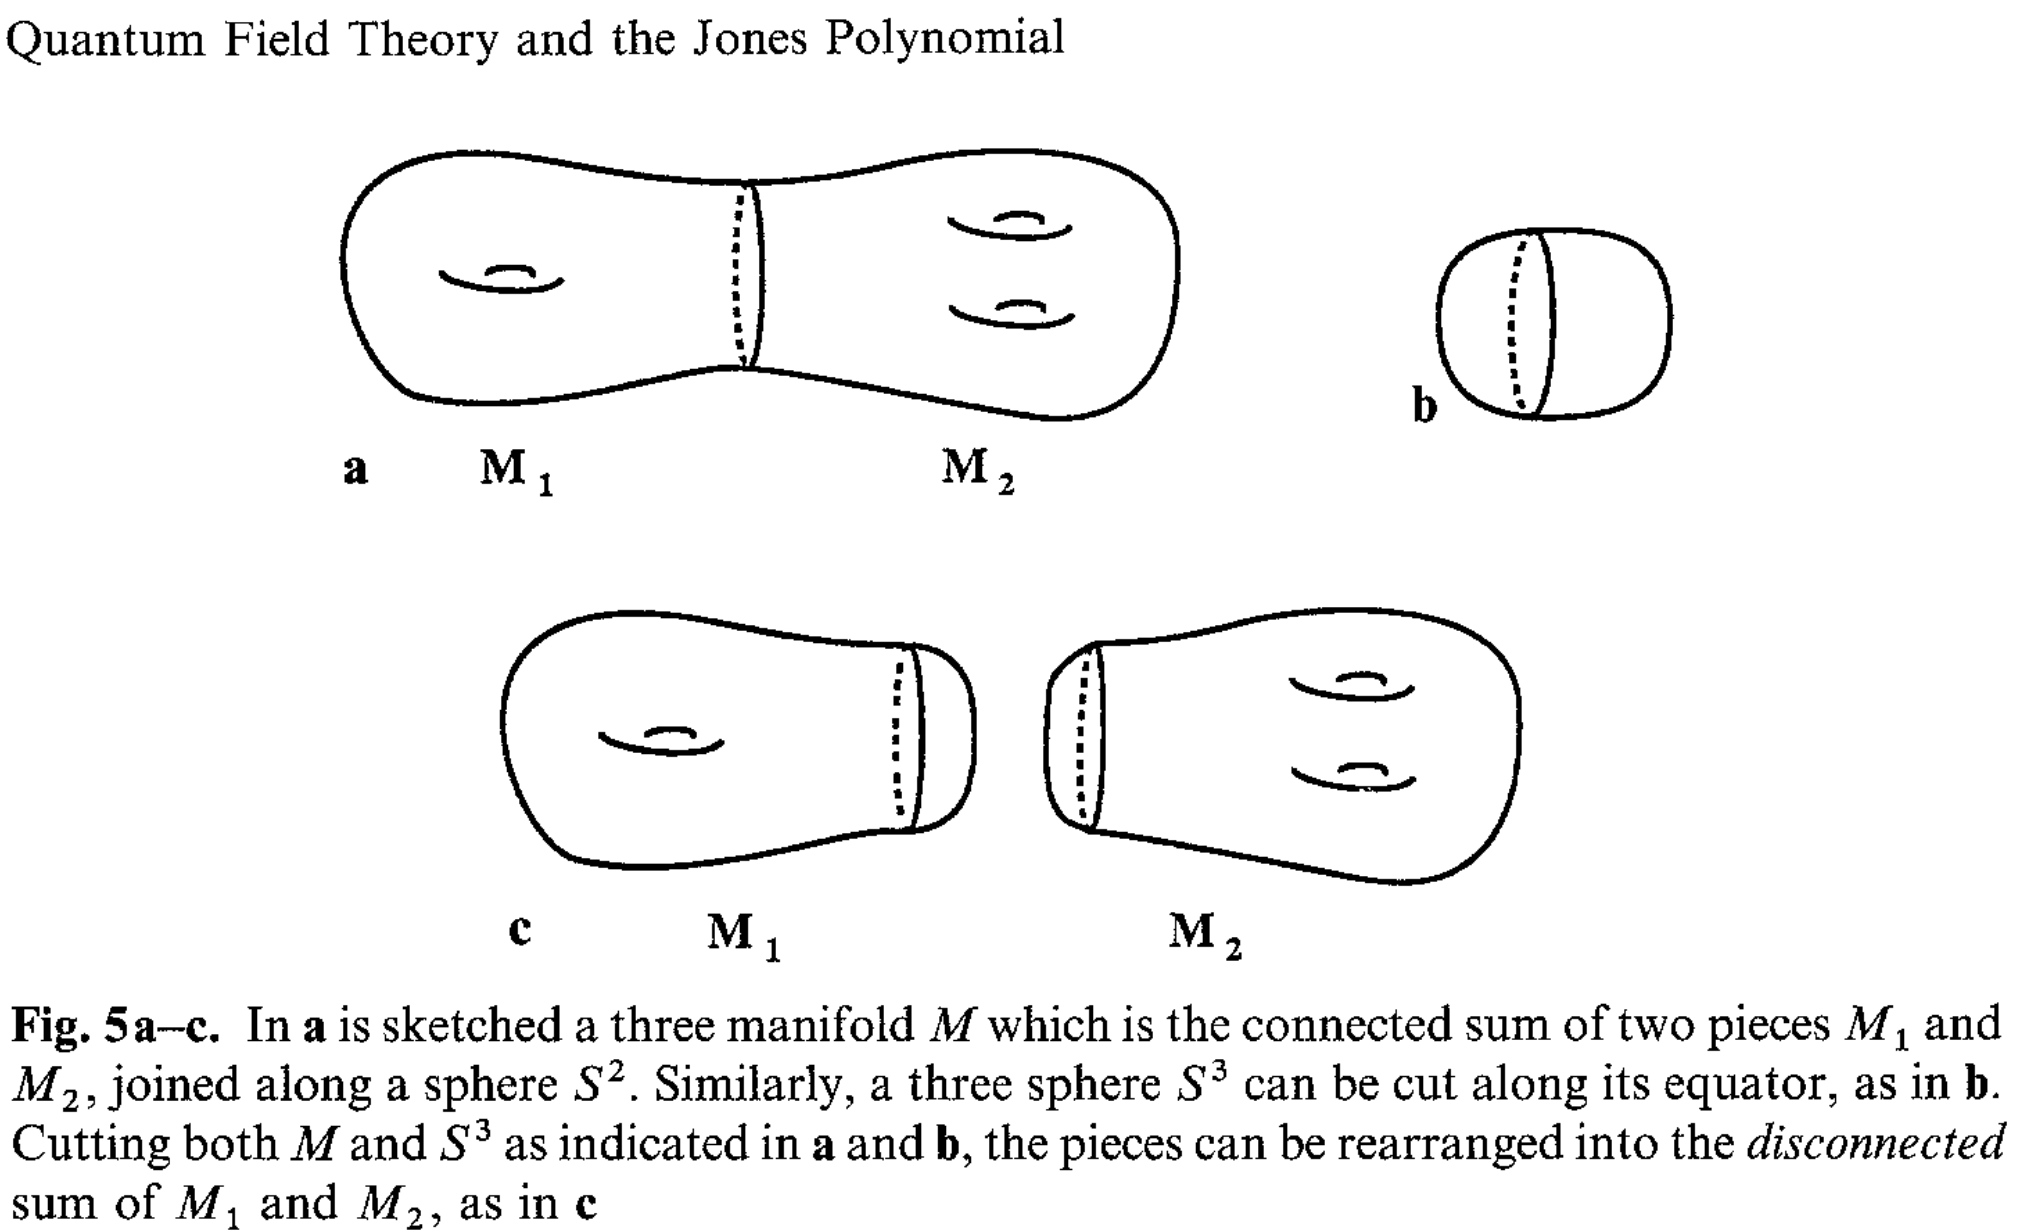
\includegraphics[width=10cm]{images/Lecture 1/witten.png}
\end{center}
Two mathematicians, Segal and Atiyah, recognized a hidden symmetric monoidal functor and pinned down  Witten's intuitions rigorously, thereby axiomatizing TQFTs (and CFTs).

\section{Topology}
\begin{flushleft}
\textit{Topology is the science of fundamental patterns\\
and structural relationships of event constellations.\\
-Fuller}
\end{flushleft}
The ideas behind cobordisms were developed already by Poincaré together with homology (and their group structure was discovered and investigated by Emmy Noether) but a proper definition was established by Pontryangin and Thom in the 20$^{\text{th}}$ century.

The strategy in general in (algebraic) topology is to probe a topological space by mapping into it, a way of viewing things very reminiscent of the Yoneda Lemma.
In the case of (singular) homology, we map simplices into the space of interest $S$. These maps are indexed by the dimension of the simplex as in the following figure.
\begin{figure}[!ht]
\centering
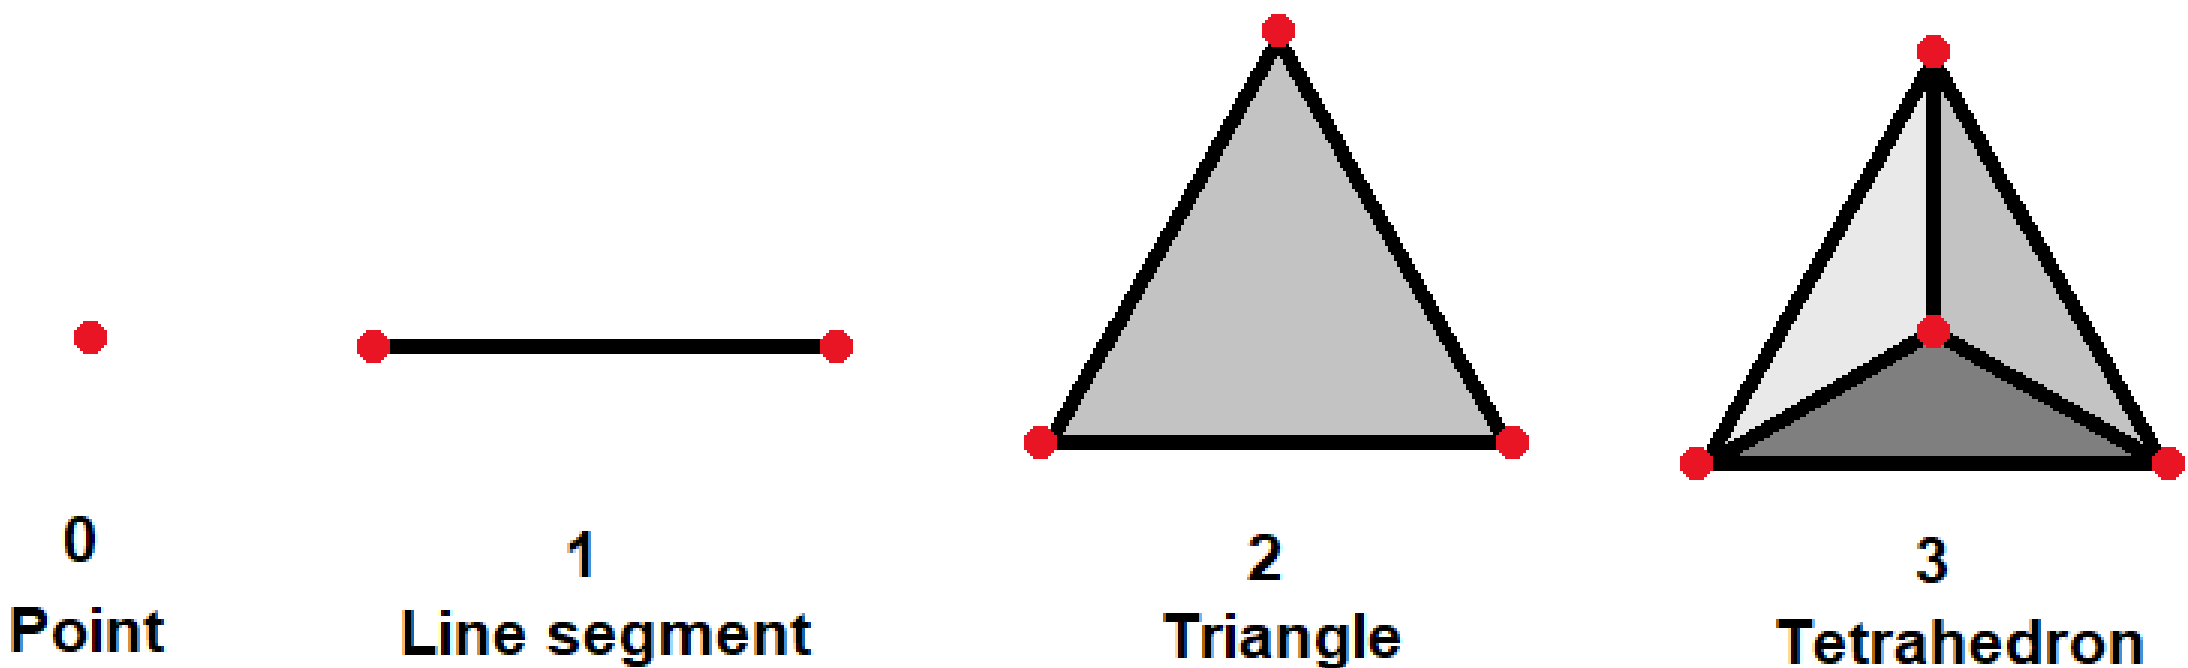
\includegraphics[width=6.5cm]{images/Lecture 1/simplex.png}
\end{figure}
We want to construct an algebraic structure around these maps $\sigma^{(n)}:\Delta^n\to S$ and so we  choose a set of coefficients, say $\R$, and construct the set of ``formal (finite) sums''  of $n$-simplices as
$$\sum a_i\sigma^{(n)}_i  ,$$
with $a_i\in\R$ and call this set $C_n(S)$. This is now an $\R$-Vector Space generated by the simplices. On the set of simplices we can introduce a map $\partial$, often called the differential or boundary, that takes each simplex to the alternating sum of the $n-1$ simplices that make up its boundary:
$$\partial\sigma^{(n)}:=\sum_{i=0}^{n}(-1)^i\sigma^{(n)}|_{i^{\text{th}}-boundary} \ ,$$
and then extend it linearly to $C_n(S)$. Calling $\partial_n:=\partial|_{C_n(S)}$, we have $\partial_n:C_n(S)\to C_{n-1}(S)$ and it can also be shown that $\partial_n \circ\partial_{n+1}=0$, a property which is often simply written as $\partial^2=0$. This defines a chain complex structure.
Given this property of $\de$, note that $\text{im}(\partial_{n+1})\subset \text{ker}(\partial_n)$ and therefore, we can define the $n^{\text{th}}$ homology of $S$ as
\begin{equation*}
    H_n(S)=\Big\{c^{(n)}: \ \ \partial_n c^{(n)}=0\Big\}\big{/}\Big\{f^{(n)}: \ \ f^{(n)}=\partial_{n+1} (f'^{(n+1)})\Big\}=\frac{\text{ker}(\partial_n)}{\text{im}(\partial_{n+1})},
\end{equation*}
and this is a vector space (by construction).
\begin{figure}[!ht]
\centering
\captionsetup{labelformat=empty, format = hang}
\begin{measuredfigure}
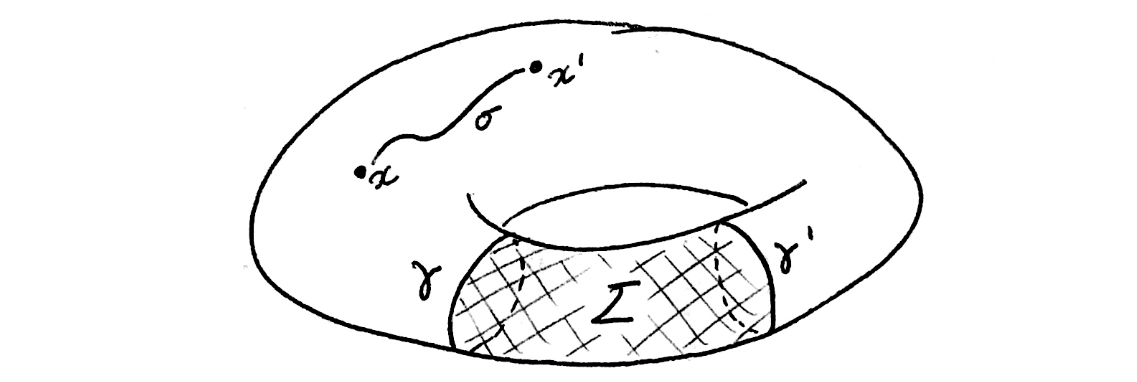
\includegraphics[width=10.40cm]{images/Lecture 1/homology.jpeg}
\caption{\small{Note that $x-x'=\partial\sigma$ so $x$ and $x'$ define the same element in $H_0$, similarly $\gamma-\gamma'=\partial\Sigma$ so that $\gamma$ and $\gamma'$ define the same element in $H_1$.}}
\end{measuredfigure}
\end{figure}

The elements of $H_1(S)$ and $H_2(S)$ can be characterized in different ways:
\begin{enumerate}
    \item The elements of $H_1(S)$ can be represented by a collection of oriented loops mapped in $S$.
    $$\amalg \ S^1\longrightarrow S$$
    \item The elements of $H_2(S)$ can be represented by a collection of maps from closed oriented surfaces (e.g. genus $g-$surfaces) in $S$.
    $$\amalg \ \Sigma\longrightarrow S$$
    \item Let $c\in H_1(S)$, then $\partial c=0$. Now by $1.$ this is some map $c: \amalg \ S^1\to S$ which is $0 \in H_1(S)$ if and only if it extends to a map $\tilde c$ of oriented surfaces in $S$, i.e. if there is the map on the bottom right such that the following diagram commutes.
    $$
    \begin{tikzcd}[row sep=tiny, column sep=small]
      \amalg \ S^1 \ar[drrr, "c"] \ar[dd, hook]\\
                  &&&S \\
      \amalg \ \Sigma \ar[urrr, dashrightarrow, "\tilde c"']
    \end{tikzcd}
    $$
    
    A drawing might be helpful:
    \begin{figure}[!ht]
    \centering
    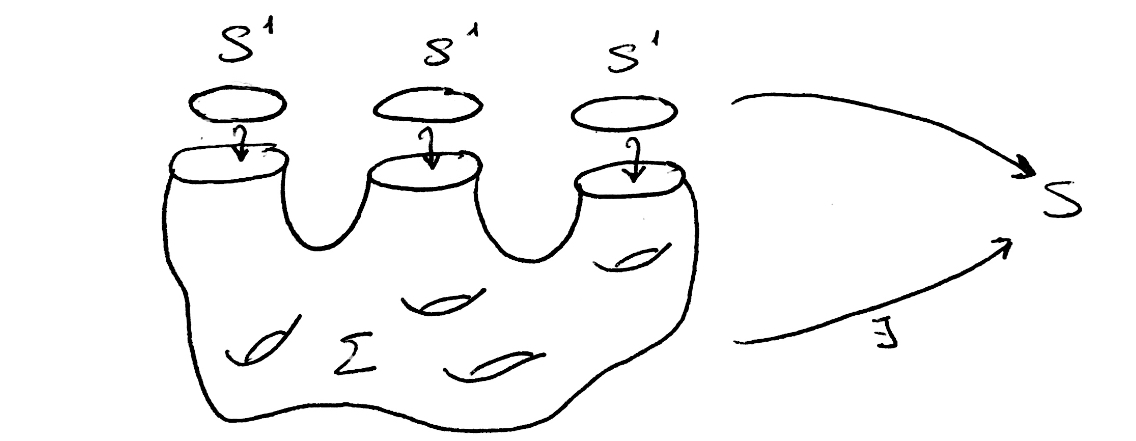
\includegraphics[width=11cm]{images/Lecture 1/extension.png}
    \end{figure}
\end{enumerate}
Can we then construct something like homology but characterized more like this last property?
This is exactly the idea of \textit{(co)bordism}:
\begin{enumerate}
    \item Let $M^n$ be a $n-$dimensional smooth compact manifold generally with boundary. Now, instead of maps from simplices we consider maps
    $$M^n\xrightarrow{f} S.$$
    \item Instead of the boundary map of simplices we consider something like:
    $$\partial\big(M^n\xrightarrow{f}S\big)=\big(\partial M^n\xrightarrow{f|_{\partial M^n}}S\big),$$
    where, if $\partial M^n=\emptyset$ then define the map to be $0$.
    \item Let $H^{\text{bord}}_n(S)$ denote this ``homology theory'' of degree $n$ on the space $S$. Let $M^n$ be closed, then $M^n\xrightarrow{f} S$ is zero in $H^{\text{bord}}_n(S)$ if and only if the map $f$ extends to a $(n+1)-$dimensional smooth compact manifold $W$ such that $\partial W= M$.
\end{enumerate}
Using these ideas one obtains something very similar to singular homology even though different, indeed this bordism theory constitutes a generalized homology theory\footnote{There exist a list of axioms called \textit{Eilenberg–Steenrod axioms} that is used to define what a homology theory is since it may come in different flavours. A generalized homology theory is a theory that has every property required but one, generally (as in the case of Bordism as seen below) that one is the \textit{dimension axiom}.}! 

\medskip

In particular, consider the one point space $S=\{*\}=pt$. What are elements in $H^{\text{bord}}_n(pt)$?

\noindent Consider a closed manifold $M^n$. This defines a class in $H^{\text{bord}}_n(pt)$ since $\de M^n = \emptyset$. Now, this is $0 \in H^{\text{bord}}_n(pt)$ if we can find a compact $n+1$ manifold $W^{n+1}$ and maps into $pt$ such that the following diagram commutes
\begin{equation*}
    \begin{tikzcd}
        M^n \arrow[dd,  hook] \arrow[rd, dashed]                         \\
                                                & pt \\
        W^{n+1} \arrow[ru, dashed] 
    \end{tikzcd}
\end{equation*}
however the maps into $pt$ are trivial and carry no extra information. 
Now, ``surely'' not all closed manifolds are a boundary of compact manifold! And so we can be sure that, in general, $H^{\text{bord}}_n(pt)\neq0$ for $n>0$.

\medskip

But when do two $n$ manifolds represent the same class in $H^{\text{bord}}_n(S)$? In the case of $S = pt$, they should be the boundary of the same manifold. In general, we require also that the maps into $S$ extend to the $n+1$ manifold, i.e. let $M_1$ and $M_2$ be closed $n$ manifolds, with maps $M_1\xrightarrow{f_1}S$ and $M_2\xrightarrow{f_2}S$, then they represent the same element in $H^{\text{bord}}_n(S)$ if and only if there exists a compact $n+1$ manifold with boundary $W$ with a map $ W\xrightarrow{g}S$ with the property that $\partial W= M_1 \amalg M_2$ and such that it makes the following diagram commute
    $$
    \begin{tikzcd}
M_1 \arrow[rd, hook] \arrow[rrd, bend left, "f_1"' description]         \\
                                        & W \arrow[r, "g"] & S \\
M_2 \arrow[ru, hook] \arrow[rru, bend right, "f_2" description]         
\end{tikzcd}
    $$
Pictorially
\begin{figure}[!ht]
\centering
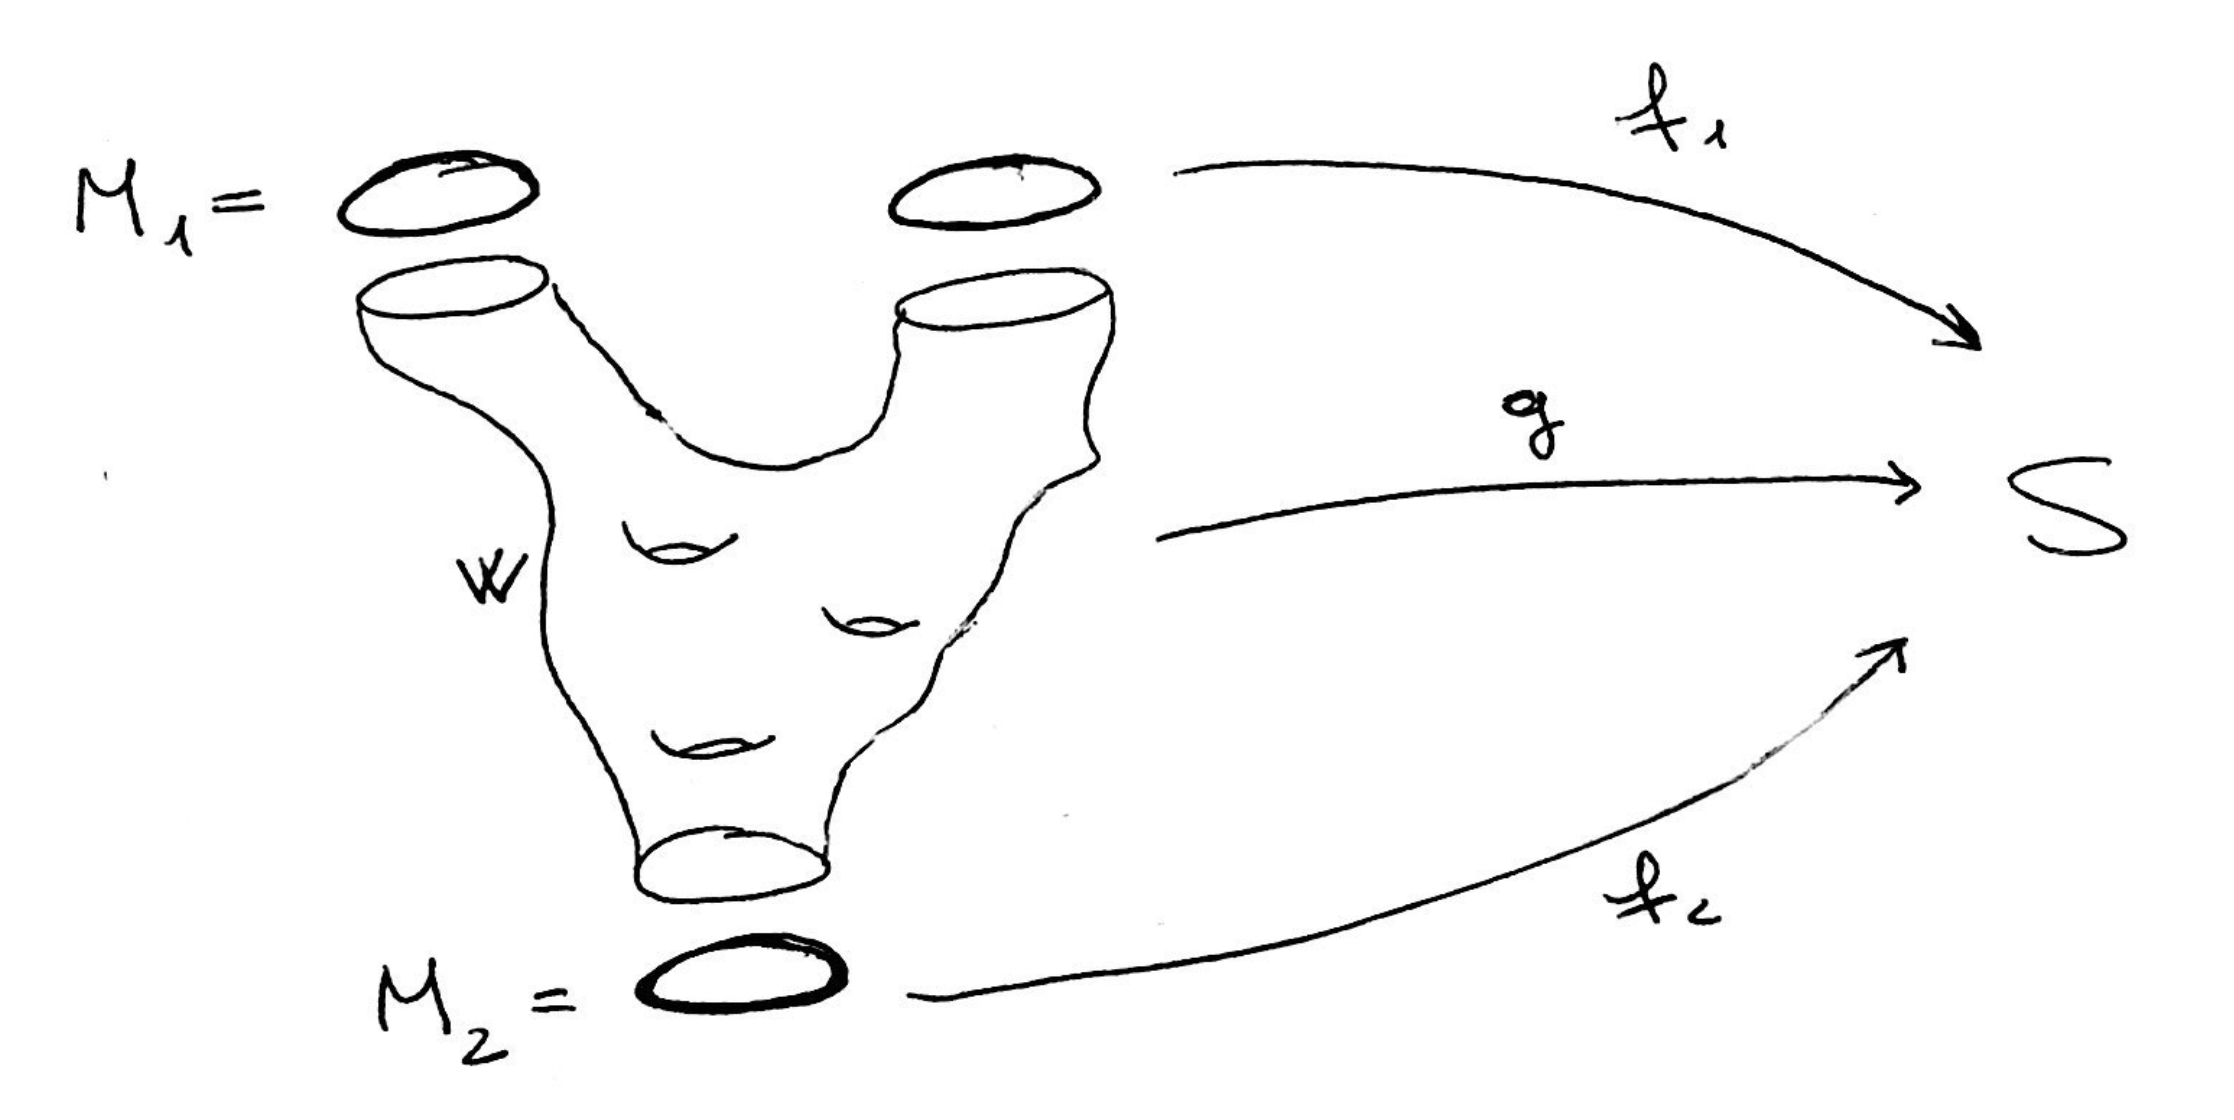
\includegraphics[width=10cm]{images/Lecture 1/cobordism.png}
\end{figure}
We then say that $M_1$ and $M_2$ are \textit{cobordant} and $W$ is called a \textit{bordism} from $M_1$ to $M_2$. 

Restricting to $S= pt$ allows us to define the \textit{Cobordism Group}
$$\Omega_n=
H^{\text{bord}}_n(pt)=
\bigg\{\text{Closed $n$ manifold}\bigg\}
\bigg{/}
\biggl\{(n+1)\text{ dimensional bordisms}
%\begin{array}{l}
%\text{Cobordant Compact}\\
%\text{$(n+1)$ manifolds}
%\end{array}
\biggl\}.$$
But are all these notions are actually useful? Well, classifying manifolds up to diffeomorphism is hard: dimension $0, 1$ and $2$ can be done without too much trouble but already in dimension $3$ things get complicated (think of the Poincaré Conjecture!)... so this classifications can be done (more easily) up to bordism!

% TBD: Could be cool to restructure a bit this subsection more geared towards TFTs rather than Bordism invariants in general because  /Andrea 

% -------------------------------------------------------------
% --------------------- LECTURE 2 25/10 -----------------------
% -------------------------------------------------------------
\part{Classical cobordism theory}
\chapter{Manifolds and bordisms}

\section{Some definitions} % (fold)
\label{sec:some_definitions}

Before venturing into a definition of cobordism, let us recall some useful definitions.
This section mainly relies on \cite{Lee2012} and \cite{Hirsch1976}.
\begin{defn}[\textit{Topological Manifold}]
	A topological manifold of dimension $n$ is a paracompact Hausdorff topological space $X$ such that every point $x \in X$ has an open neighborhood $U$ which is homeomorphic to an open set\footnote{Equivalently to $\R^n$.} in $\R^n$. The latter property means that for each $x\in X$ there exist:
    \begin{itemize}
        \item an open subset $U\subseteq X$ containing $x$, i.e. an open neighbourhood of $x$,
        \item a corresponding open subset $\tilde{U}\in\R^n$,
        \item a homeomorphism $\phi_{U} : U \to \tilde{U}=\phi(U) $ called coordinate chart, or just chart (see Fig. \ref{fig:Coordinate_Chart}).
	\end{itemize} 
 \end{defn}
\begin{figure}
    \centering
    \captionsetup{format = hang}
    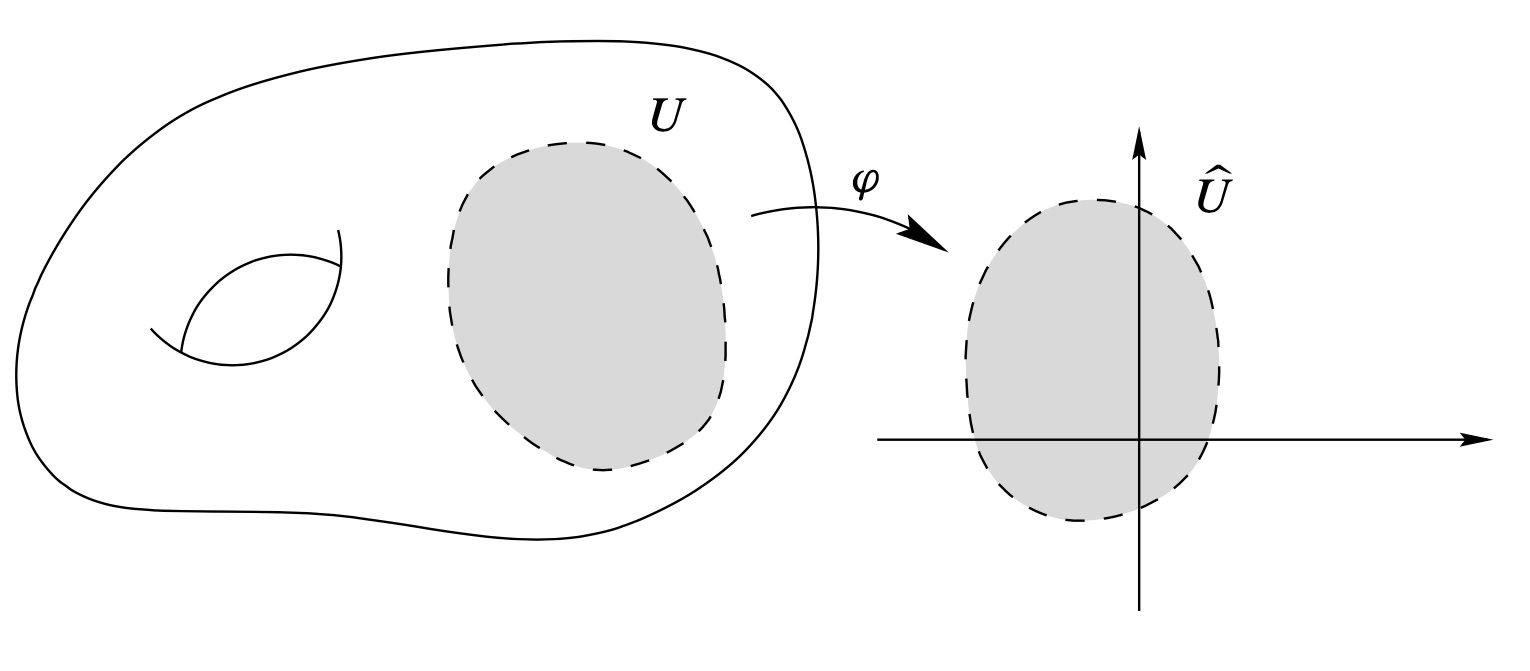
\includegraphics[width=12cm]{images/Lecture 2/Coordinate Chart.png} 
    \caption{\small{The visualization of a coordinate chart map from Lee's textbook on smooth manifolds \cite{Lee2012}}}
    \label{fig:Coordinate_Chart}
\end{figure}
\noindent If $(U, \phi)$, $(V, \psi)$ are two coordinate charts of a topological manifold $X$ and $U\cap V\neq\emptyset$, then $\psi \circ \phi^{-1} : \phi(U\cap V) \to \psi(U\cap V)$ is a transition function from $\phi$ to $\psi$ (see Fig. \ref{fig:Lee_TransitionMap}).
\begin{figure}
    \centering
    \captionsetup{format = hang}
    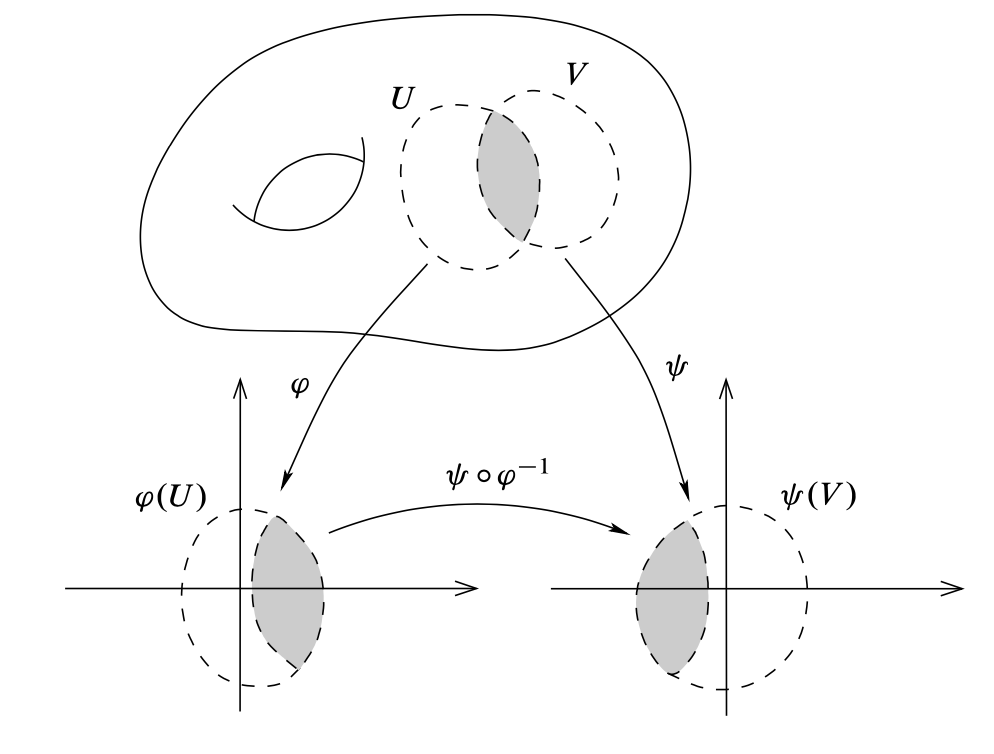
\includegraphics[width=12cm]{images/Lecture 2/Lee_TransitionMap .png} 
    \caption{\small{The picture of a transition function from \cite{Lee2012}}}
    \label{fig:Lee_TransitionMap}
\end{figure}

From the introduction it's clear that we will also deal with manifolds with boundary, so we recall also this definition. In order to do this we first introduce the following notation.
\begin{notat}[Half-space]
    By $\mathbb{H}^n$ we denote the $n$-dimensional upper (closed) half-space,
    $$\mathbb{H}^n=\{(x_1,...,x_n)\in\mathbb{R}^n|x_1 \leq 0\}$$ 
\end{notat}
\begin{defn}[Manifold with Boundary]
	A manifold with boundary of dimension $n$ is a paracompact Hausdorff topological space $X$ such that every point $p \in X$ has an open neighborhood $U_p$ which is homeomorphic to an open set $V$ in $\H^n$, i.e. the closed\footnote{in topological sense and not in the manifold sense we later define.} half space, via the homeomorphism $\phi$ of the coordinate chart $(U_p,\phi)$.
\end{defn}
\begin{figure}
    \centering
    \captionsetup{format = hang}
    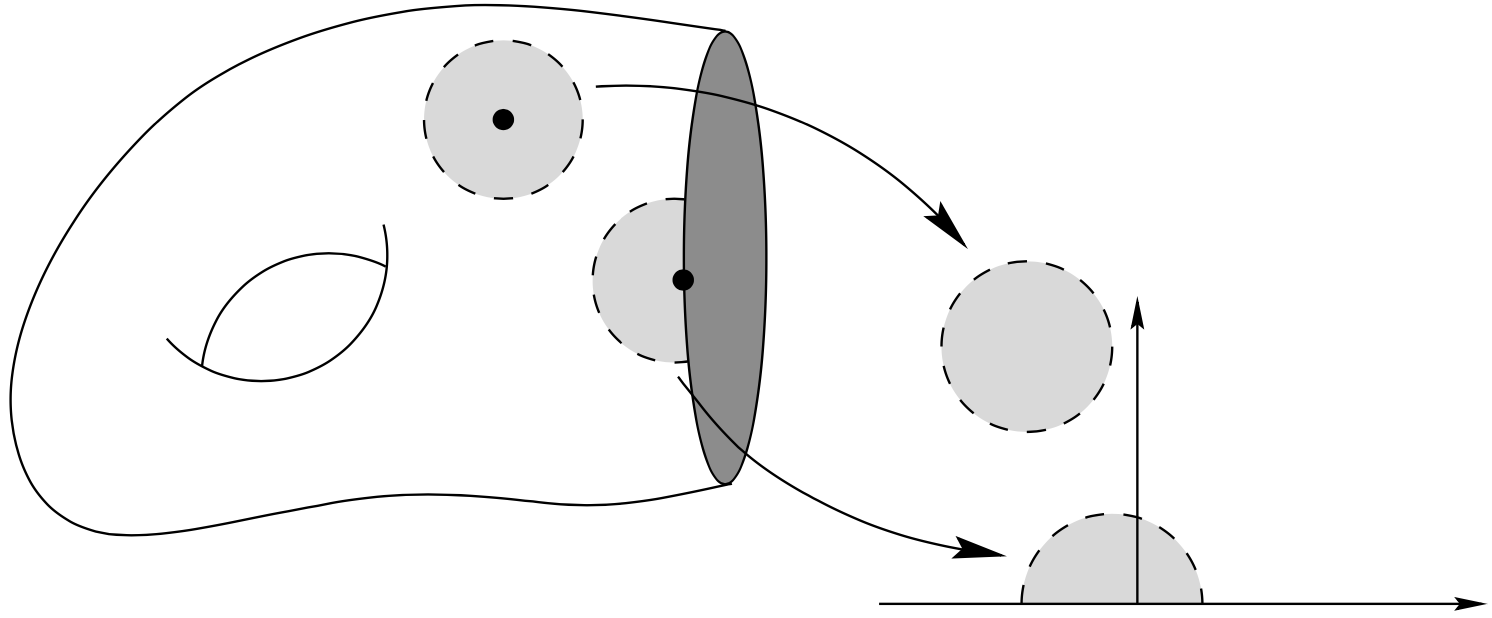
\includegraphics[width=12cm]{images/Lecture 2/Manifold with boundary.png} 
    \caption{\small{The picture of a 2-dimensional manifold with boundary from \cite{Lee2012}}}
    \label{fig:Manifold_w_boundary}
\end{figure}

\begin{defn}[Boundary of a Manifold]
	If for $p \in X$ and some chart $\phi$ it is the case that $x_1(\phi (p) )= 0$ (meaning $\phi_p (x) \in \{(0,x_2, \dots, x_n)\}\subseteq \H^n$), then it does in every chart. We then say that $p$ is in the \textit{boundary} of $X$, 
	$$
		\de X := \{ p \in X : x_1(p) = 0\}
	$$
	otherwise, $p$ is in the \textit{interior} of $X$, which we denote with Int $X$. 

    \noindent Equivalently, $p \in \de X$ means that $p$ has neighborhood $V$ that is the domain of a coordinate chart $\psi:V\to\H^n$ such that $\psi(V)\cap\de\H^n\neq\emptyset$ and sending $p$ to $\de \H^n$.

    \noindent Specularly, we could have defined the interior of $X$ to be the set of points $q\in X$ that have a neighourhood $U$ that is the domain of a chart $\psi:U\to\R^n$.
\end{defn}
\begin{lem}
    If $X$ is an $n$ dimensional manifold with boundary, then $\de X$ is a $n-1$ dimensional manifold.
\end{lem}
\begin{proof}
    Let $p\in\de X$ be an arbitrary point on the boundary of an $n$ manifold with boundary. Hence, there is an open neighbourhood $U_p$ of $p$ which is homeomorphic to an open set $V$ in $\mathbb{H}^n$, $ \phi(U_p)\cong V$. Since $p\in\de X$ we know that $x_1(\phi(p))=0$ and $\phi(p)\in V\cap\mathbb{H}^n$. $\phi:U_p\to V$ can be restricted to a homemorphism $\phi\mid_{\phi^{-1}(V\cap\mathbb{H}^n)}:\phi^{-1}(V\cap\mathbb{H}^n)\xrightarrow{\cong}V\cap\mathbb{H}^n$. Note that $\phi^{-1}(V\cap\mathbb{H}^n)=U_p\cap\de X$ because $p$ is sent to the boundary $\de\mathbb{H}^n$ for every chart. Note also that $\de\mathbb{H}^n=\{(0,x_2, \dots, x_n)\}$ and $\de\mathbb{H}^n\cong\R^{n-1}$. Since $V\cap\mathbb{H}^n\in\de\mathbb{H}^n$ and $V\cap\mathbb{H}^n\cong U_p\cap\de X$, $U_p\cap\de X$ is homeomorphic to an open set in $\R^{n-1}$.
\end{proof}
\begin{defn}[Closed Manifold]
    A manifold is \textit{closed} if it is compact and without boundary, i.e. $\de X = \emptyset$. Conversely, an \textit{open} manifold is also a manifold without boundary but with no closed components, i.e. it has only non-compact components. 
\end{defn}

In some contexts, it can be interesting to do calculus on a manifold. In order to make sense of this, one needs to add some extra structure to the topology of the manifold which enables investigating if a map between manifolds is smooth.
\begin{defn}[Smooth Function]
    Given $X\subseteq\R^n$ and $Y\subseteq\R^m$ a function $f:X\to Y$ is smooth\footnote{Also called infinitely differentiable or $C^\infty$.} if each of its component functions has continuous partial derivatives of all order.
\end{defn}

\noindent The right notion of isomorphism when talking about smooth functions is that of diffeomorphism:
\begin{defn}[Diffeomorphism]
    A smooth map $f:X\rightarrow Y$ is a diffeomorphism when it is bijective and has a smooth inverse map.
\end{defn}

\begin{defn}[Smooth Manifold Without Boundary]
	A smooth manifold $X$ is a topological manifold, together with a collection of charts $\phi_i:U_i\to\R^n$, called smooth structure, $(U_i, \phi_i)$ such that:
	\begin{enumerate}
		\item $X = \bigcup_{i\in I} U_i$
		\item the pairwise transition functions are smooth in the usual sense of $\R^n$
  %what does 'pairwise' transition functions mean? Isn't 'transition functions and their inverses' clearer? /Andrea
		\item it is maximal with respect to 1. and 2.
	\end{enumerate}
 Some call a collection of charts $(U_i, \phi_i)$ such that $\{U_i\}_i\in I$ is a cover of the whole manifold $X$ an atlas. A smooth atlas is an atlas where the transition functions and their inverses are smooth. A smooth structure is thus a maximal smooth atlas. We call charts forming the smooth structure smooth charts.
\end{defn}

\begin{ex}
	A lot of the spaces we think of are smooth manifolds, such as:
	\begin{enumerate}
		\item the circle, a dimension 1 manifold
		\item a genus $g$ surface, a dimension 2 manifold
		\item $\emptyset$, a smooth manifold of any dimension
	\end{enumerate}
\end{ex}
\begin{notat}
    In these lecture notes, manifolds are \textit{always} smooth, unless explicitly specified.
\end{notat}
\begin{rem}
    The definition of smoothness we just provided does not work for manifolds with boundary since to say that the transition functions are smooth we used the notion of smoothness of $\R^n$ and not of $\H^n$, the actual codomain of manifolds \emph{with} boundary. Hence, we characterize now smoothness for $\H^n$.
\end{rem}

\noindent Recall that a map $f:M\to\R^m$, where $M\subseteq \R^n$ is not necessarily open, is smooth if in a neighbourhood of each $x\in M$ it can be extended to a smooth function defined on an open subset in $\R^n$. 

\begin{defn}[Smoothness in the Half Space]\label{SmoothHalf}
    If $X$ is an open subset of $\H^n$, we define $f:X\to\R^m$ to be smooth for each $x\in X$ if $X$ can be extended to an open subset $\tilde{X}\in\R^n$, and $f$ to a smooth map $\tilde{f}:\tilde{X}\to\R^m$ such that $\tilde{f}|_{\tilde{X}\cap\H^n}=f$. 
\end{defn}

\begin{defn}[Smooth Manifold with Boundary]
    A topological manifold with boundary is smooth if it has a maximal smooth atlas where the transition functions and their inverses are smooth according to \ref{SmoothHalf}.
\end{defn}

\begin{cor}
    If $X$ is a smooth $n$ dimensional manifold with boundary, then $\de X$ is a smooth $n-1$ dimensional manifold. It follows from the proof for topological manifolds.
\end{cor}
	 
\begin{ex}% see how to go on another line for the first item. Solutions: \item[], \leavevmode, \hfill
\hfill 
\begin{enumerate}
	\item $D^n = \{x \in \R^n \mid  \ ||x||\leq 1\}$ the $n$ dimensional disk, which has a sphere as boundary: $\de D^n = S^{n-1}$
	\[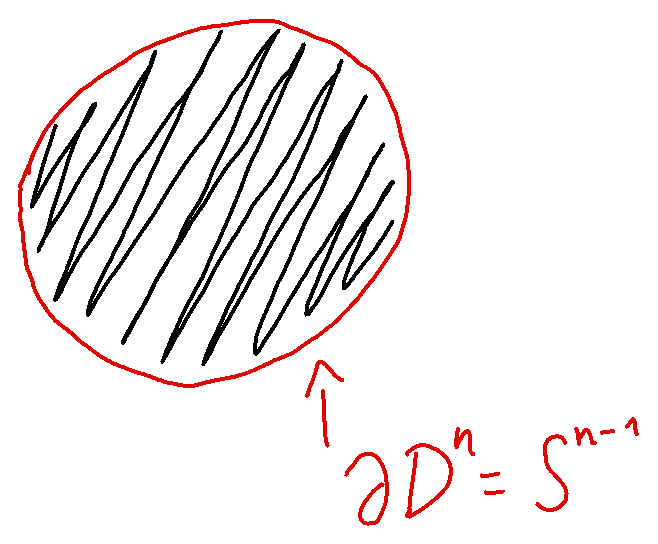
\includegraphics[width=5cm]{images/Lecture 2/Boundary Disk.png} \]
	\item Consider 2 dimensional \emph{open} disks, i.e. $D^2=\{x\in\R^2\mid \ ||x||<1\}$. We can remove such shapes
	 from the sphere and get the manifold $S^{2} \setminus D^{2}_{1} \amalg D_2^2 \amalg D^2_3$ which we can
	  visualize in different ways. \[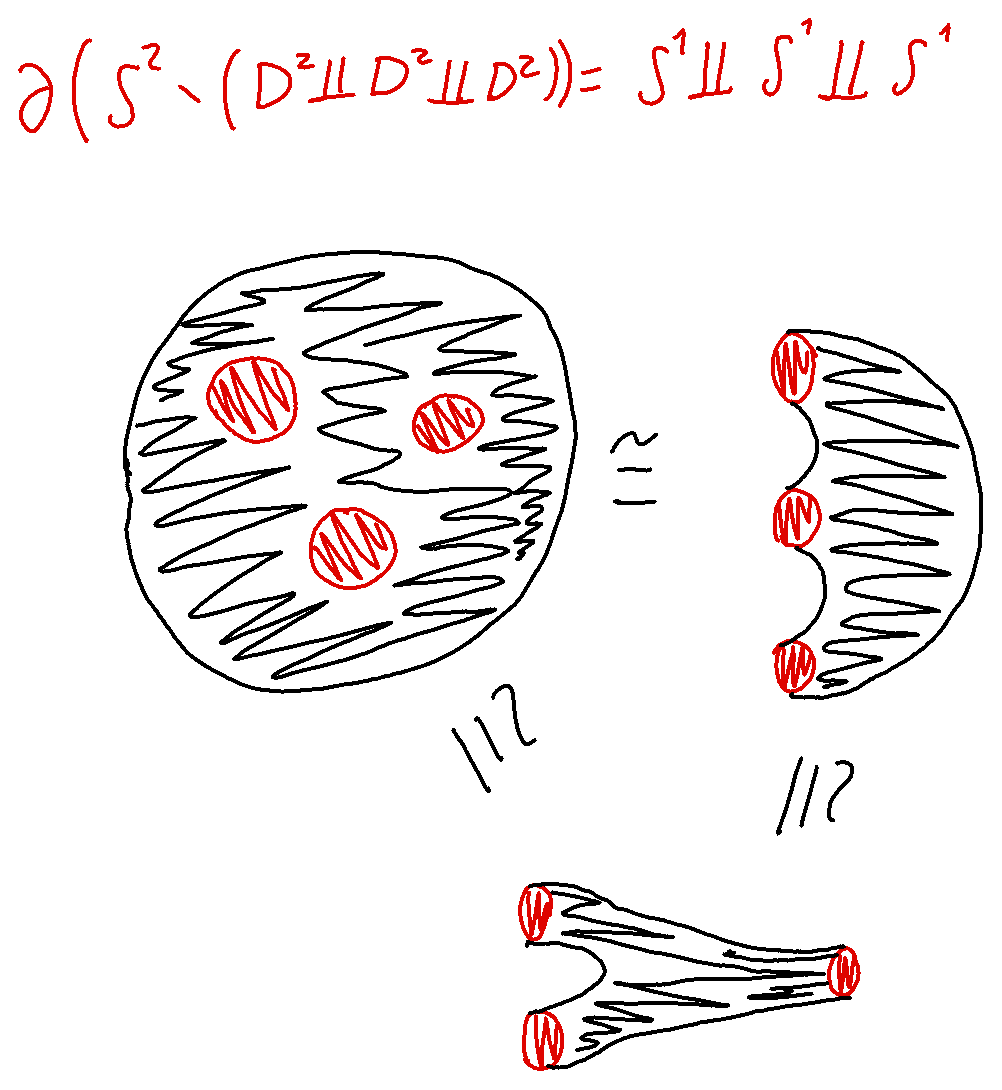
\includegraphics[width=7cm]{images/Lecture 2/Manifold3holes.png} \]
	\item Let $X, Y$ be $n$ manifolds with boundary, then $X \amalg Y$ is an $n$ manifold with boundary.
	\[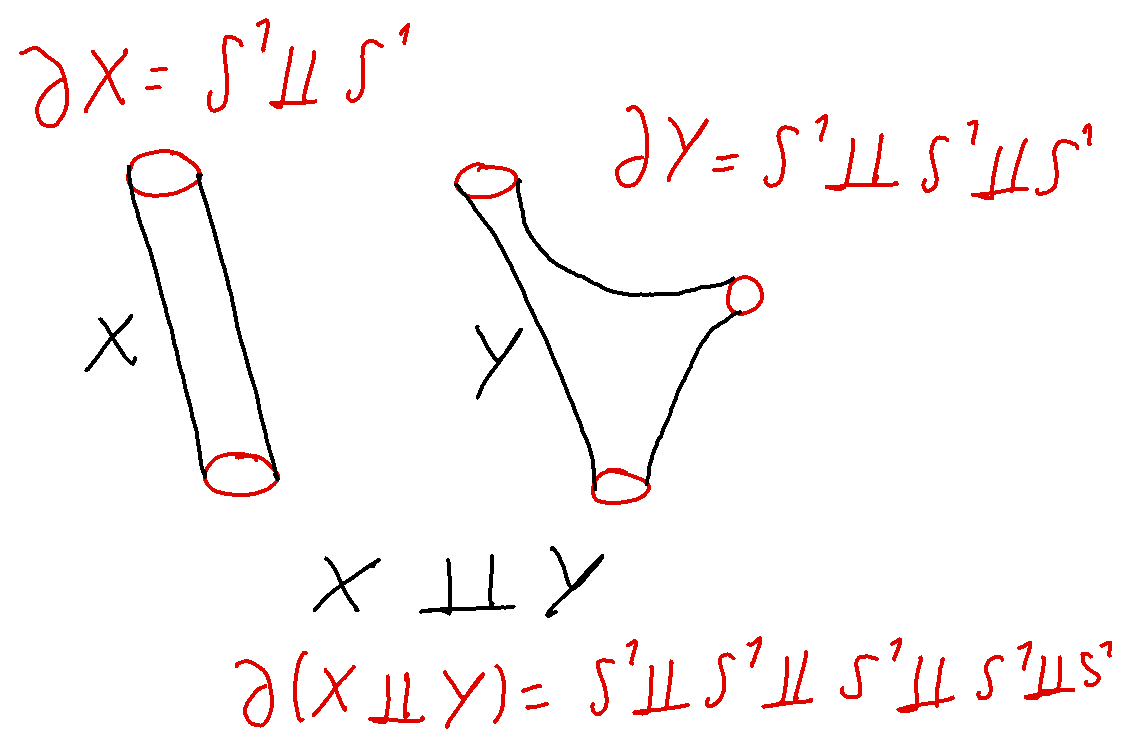
\includegraphics[width=7cm]{images/Lecture 2/Disjoint union of manifolds with boundary.png} \]
	\item $T= S^1 \times S^1$ is a $2$ manifold with $\de T = \emptyset$ and $T^{\text{solid}} = D^2 \times S^1$ is a $3$-manifold with $\de T^{\text{solid}} = T$.
		\[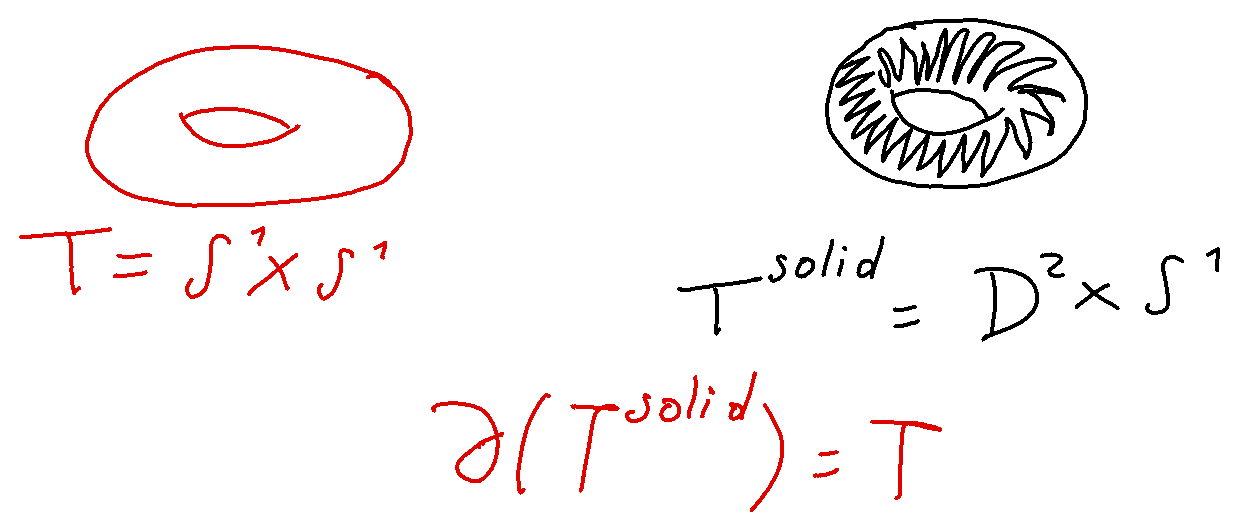
\includegraphics[width=7cm]{images/Lecture 2/Torus Boundary.png} \]
	\end{enumerate}
\end{ex}

\begin{defn}[Smooth Map to $\R^n$]
    Let $X$ be a smooth manifold. $f:X\to\R^n$ is smooth if for each $x\in X$ there is a smooth chart $(U,\phi)$ such that $f=f\circ\phi^{-1}$
\end{defn}

\noindent This definition can be generalized to maps between smooth manifolds.

\begin{defn}[Smooth Map between Manifolds]
    Let $X$ and $Y$ be smooth manifolds of dimensions $m$ and $n$ and $f:X\to Y$ a function between them. $f$ is smooth if for every $x\in X$ there is a smooth chart $(U,\phi)$ of $X$ where $x\in U$ and a smooth chart $(V,\psi)$ of $Y$ where $f(x)\in V$ and $f(U)\subseteq V$ such that $\tilde f = \psi \circ f\circ \phi^{-1}$ is smooth. $\tilde f$ can be represented as in the following diagram:
    \begin{equation*}
        \begin{tikzcd}
            {X\supseteq U} &&& {V\subseteq Y} \\
            &&& {} \\
            {\mathbb{H}^m\supseteq\tilde{U}} &&& {\tilde{V}\subseteq\mathbb{H}^n}
            \arrow["f|_U", from=1-1, to=1-4]
            \arrow["{\psi_x}", from=1-4, to=3-4]
            \arrow["{\tilde{f}}"', from=3-1, to=3-4]
            \arrow["\cong"', from=1-4, to=3-4]
            \arrow["{\phi_x}"', from=1-1, to=3-1]
            \arrow["\cong", from=1-1, to=3-1]
        \end{tikzcd}
    \end{equation*}
\end{defn}
\noindent This also allows to define the natural notion of isomorphism in the category of smooth manifolds:
\begin{defn}[Diffeomorphism of Manifolds]
    A diffeomorphism is a smooth map with a smooth inverse, i.e. an isomorphism in the category of smooth manifolds.
\end{defn}

\begin{exercise}
	Come up with the natural notion of smooth map between manifolds \emph{with} boundary. 
\end{exercise}

\section{What is a Bordism?}

\begin{defn}[$1^{st}$ variant of the definition of bordism: via \emph{strict equalities}]
\label{Define Bordism}
	Let $Y_0, Y_1$ be closed $n$ manifolds. A bordism $(X,p)$ from $Y_0$ to $Y_1$ consists of a compact $n+1$ manifold with boundary together with a map $p: \de X \to \{0,1\}$ such that $Y_0 = p^{-1}(0)$ and $Y_1 = p^{-1}(1)$. Thus, $\de X = Y_0 \amalg Y_1$.

	\noindent We then say that $Y_0$ and $Y_1$ are \textit{cobordant}.
\end{defn}
\noindent We call $Y_0$ the \textit{incoming} boundary and $Y_1$ the \textit{outgoing} boundary. We sometimes write $\de_{in} X = Y_0$ and $\de_{out} X = Y_1$.

\begin{ex}
	``pair of pants'' %DRAWING
    \begin{figure}[!ht]
        \centering
        \captionsetup{labelformat=empty, format = hang}
        \begin{measuredfigure}
            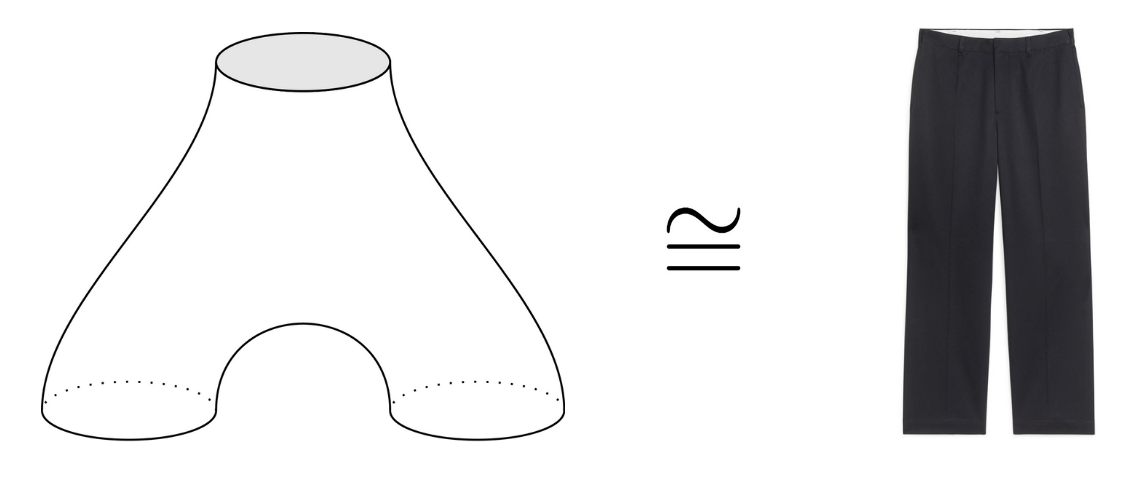
\includegraphics[width=9cm]{images/Lecture 2/pants_topological.png} 
            \caption{\small{Bordism from $S^1$ to $S^1\amalg S^1$}}
        \end{measuredfigure}
    \end{figure}
\end{ex}

\begin{ex} 
\hfill
\begin{itemize}
    \item The torus is a bordism from $\emptyset$ to $\emptyset$. ($\de T = \emptyset = Y_0 \amalg Y_1 \implies Y_0 = Y_1 = \emptyset$)
    %\begin{figure}[!ht] % Torus as a bordism: empty -> empty
        %\centering
    \begin{center} % changed it to this so the picture is exactly here
        \begin{tikzpicture}
            \node (A) at (-3,0) {};
            \node (B) at (-3,-2){\small{$Y_0 = \emptyset$}};
            \draw[->] (A)--node[auto, align=center]{}(B);
            
            \pic{torus={2cm}{5.6mm}{70}};

            \node (C) at (3,0) {};
            \node (D) at (3,-2){\small{$Y_1 = \emptyset$}};
            \draw[->] (C)--node[auto, align=center]{}(D);
        \end{tikzpicture}
    \end{center}
    %\end{figure}\vspace{-6mm}
    %
    \item	$X = S^1 \times [0,1]$, now $\de X = S_1 \amalg S_1$ and we can view it as a bordism in 4 ways:
    \begin{figure}[H]
    \centering
    \begin{subfigure}[t]{.4\textwidth}
        \centering
        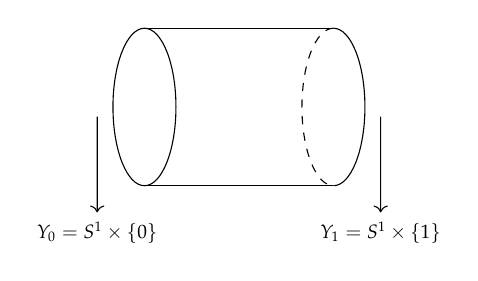
\begin{tikzpicture}[scale=0.8]
            \tikzmath{\cylH = 3; \cylr = 0.5; \cylR = 1.25; \spc = 0.75;} 
            \node (A) at (-\spc, 0) {};
            \node (B) at (-\spc, -\cylR - \spc){\scriptsize{$Y_0 = S^1\times\{0\}$}};
            \draw[->] (A)--node[auto, align=center]{}(B);
            
            \draw (0, 0) ellipse ({\cylr} and {\cylR});
            \draw (0, \cylR) -- (\cylH, \cylR);
            \draw (0, -\cylR) -- (\cylH, -\cylR);
            \draw [dashed] (\cylH, \cylR) arc (90:270:{\cylr} and {\cylR});
            \draw (\cylH,\cylR) arc (90:270:{-\cylr} and {\cylR});

            \node (C) at (\cylH + \spc, 0) {};
            \node (D) at (\cylH + \spc, -\cylR - \spc){\scriptsize{$Y_1 = S^1\times\{1\}$}};
            \draw[->] (C)--node[auto, align=center]{}(D);
        \end{tikzpicture}
    \end{subfigure}
    \hspace{5mm}
    \begin{subfigure}[t]{.4\textwidth}
        \centering
        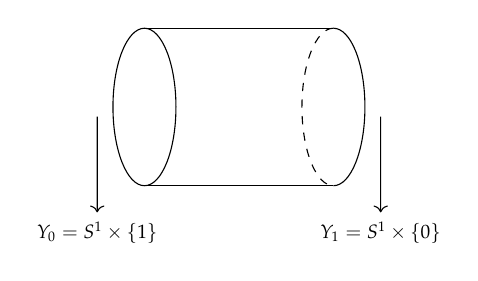
\begin{tikzpicture}[scale=0.8]
                \tikzmath{\cylH = 3; \cylr = 0.5; \cylR = 1.25; \spc = 0.75;} 
                \node (A) at (-\spc, 0) {};
                \node (B) at (-\spc, -\cylR - \spc){\scriptsize{$Y_0 = S^1\times\{1\}$}};
                \draw[->] (A)--node[auto, align=center]{}(B);
                
                \draw (0, 0) ellipse ({\cylr} and {\cylR});
                \draw (0, \cylR) -- (\cylH, \cylR);
                \draw (0, -\cylR) -- (\cylH, -\cylR);
                \draw [dashed] (\cylH, \cylR) arc (90:270:{\cylr} and {\cylR});
                \draw (\cylH,\cylR) arc (90:270:{-\cylr} and {\cylR});
    
                \node (C) at (\cylH + \spc, 0) {};
                \node (D) at (\cylH + \spc, -\cylR - \spc){\scriptsize{$Y_1 = S^1\times\{0\}$}};
                \draw[->] (C)--node[auto, align=center]{}(D);
        \end{tikzpicture}
    \end{subfigure}

    \medskip
        
    \begin{subfigure}[t]{.4\textwidth}
        \centering
        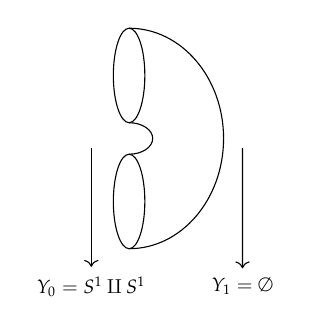
\begin{tikzpicture}[scale=0.8]
            \tikzmath{\cylH = 3; \cylr = 0.25; \cylR = 0.75; \spc = 0.6; \gp = 0.5;} 
            \node (A) at (-\spc, -\cylR - \gp/2) {};
            \node (B) at (-\spc, -3 * \cylR - \gp -\spc){\scriptsize{$Y_0 = S^1\amalg S^1$}};
            \draw[->] (A)--node[auto, align=center]{}(B);
            
            \draw (0, 0) ellipse ({\cylr} and {\cylR});
            \draw (0, -2 * \cylR - \gp) ellipse ({\cylr} and {\cylR});
            
            \draw (0,-\cylR) arc (90:270:{-1.5*\cylr} and {\cylr});
            \draw (0,\cylR) arc (90:270:{-2*\cylR} and {2*\cylR + \gp/2});
    
            \node (C) at (2*\cylR + \spc/2, -\cylR - \gp/2) {};
            \node (D) at (2*\cylR + \spc/2, -3 * \cylR - \gp -\spc){\scriptsize{$Y_1 = \emptyset$}};
            \draw[->] (C)--node[auto, align=center]{}(D);
        \end{tikzpicture}\hspace{10mm}
    \end{subfigure}
    \begin{subfigure}[t]{.4\textwidth}
        \centering
        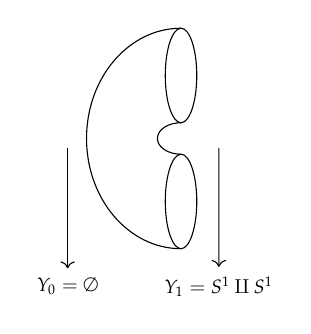
\begin{tikzpicture}[scale=0.8]
            \tikzmath{\cylH = 3; \cylr = 0.25; \cylR = 0.75; \spc = 0.6; \gp = 0.5;} 
            \node (A) at (-\spc / 2, -\cylR - \gp/2) {};
            \node (B) at (-\spc / 2, -3 * \cylR - \gp -\spc){\scriptsize{$Y_0 = \emptyset$}};
            \draw[->] (A)--node[auto, align=center]{}(B);
            
            \draw (2*\cylR, 0) ellipse ({\cylr} and {\cylR});
            \draw (2*\cylR, -2 * \cylR - \gp) ellipse ({\cylr} and {\cylR});
            
            \draw (2*\cylR,-\cylR) arc (90:270:{1.5*\cylr} and {\cylr});
            \draw (2*\cylR,\cylR) arc (90:270:{2*\cylR} and {2*\cylR + \gp/2});

            \node (C) at (2*\cylR + \spc, -\cylR - \gp/2) {};
            \node (D) at (2*\cylR + \spc, -3 * \cylR - \gp -\spc){\scriptsize{$Y_1 = S^1\amalg S^1$}};
            \draw[->] (C)--node[auto, align=center]{}(D);
        \end{tikzpicture}
    \end{subfigure}
    \end{figure}
    The latter two are sometimes calles 'macaroni'.
    
    This shows that different bordisms can arise from the same underlying manifold. We will have a way of differentiating them when we will introduce tangential structures on a manifold, which will enable us to explain in which direction a manifold is oriented.

    \item Given two $n$ manifolds $M,N$, their \textit{connected sum} is 
    \begin{equation*}
         M\# N=M\setminus(D^{n})^{\circ}\coprod_{S^{n-1}} N\setminus(D^{n})^{\circ}
     \end{equation*}
     where ${}^{\circ}$ is for taking the interior and $\coprod_{S^{n-1}}$ is glueing along the new boundaries in $N$ and $M$.
    \begin{figure}[!ht]
    \centering
    \captionsetup{labelformat=empty, format = hang}
        \begin{measuredfigure}
            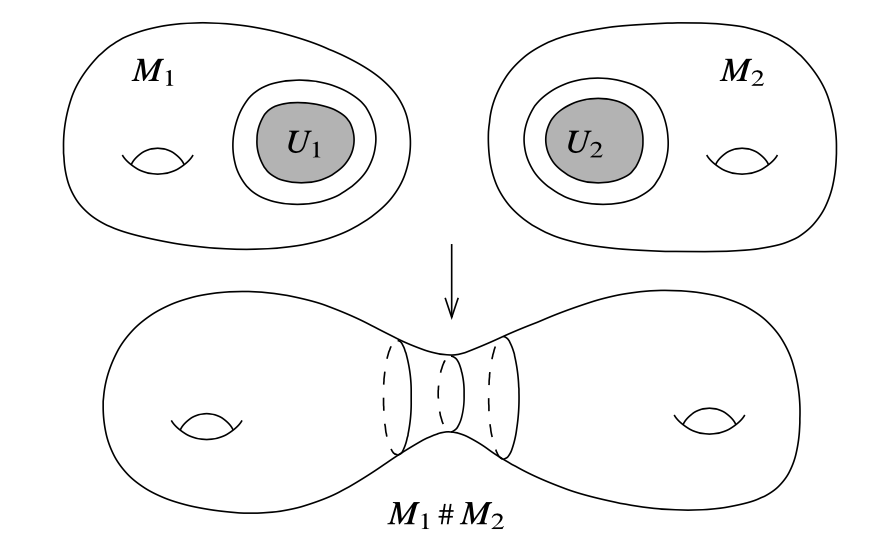
\includegraphics[width=9cm]{images/Lecture 2/connected sum.png} \caption{\small{The picture of a connected sum from \href{https://en.wikipedia.org/wiki/Connected_sum]}{Wikipedia}}}
        \end{measuredfigure}
    \end{figure}
\end{itemize}
\end{ex}
\begin{prop}
    $M\# N$ is an n manifold.
\end{prop}
%proof to be added?
\begin{lem}
    There is a bordism between $M\coprod N$ and $M\# N$.
\end{lem}

\begin{proof} 
    A bordism between $M_1\coprod M_2$ and $M_1\#M_2$ may be constructed in the following manner (proof taken from the \href{http://www.map.mpim-bonn.mpg.de/Bordism#Connected_sum_and_bordism}{Manifold Atlas Project}). Consider a cylinder $M_1\times I$, from which we remove an $\epsilon$-neighbourhood $U_{\epsilon}(v_{1}\times 1)$ of the point $v_{1}\times 1$. Similarly, remove the neighbourhood $U_{\epsilon}(v_{2}\times 1)$ from $M_{2}\times I$ (each of these two neighbourhoods can be identified with the half of a standard open $(n+1)$-ball). Now connect the two remainders of cylinders by a "half pipe" $\left(S_{n}\leq 0 \right)\times I$ in such a way that the half-sphere $S_{n}\leq 0$ is identified with the half-sphere on the boundary of $U_{\epsilon}(v_{1}\times 1)$, and $\left(S_{n}\leq 0 \right)\times I$ is identified with the half-sphere on the boundary of $U_{\epsilon}(v_{2}\times 1)$. Smoothening the angles we obtain a manifold with boundary $(M_1\coprod M_2)\coprod(M_1\#M_2)$.
\begin{figure}[H]
\centering
\captionsetup{labelformat=empty, format = hang}
    \begin{measuredfigure}
        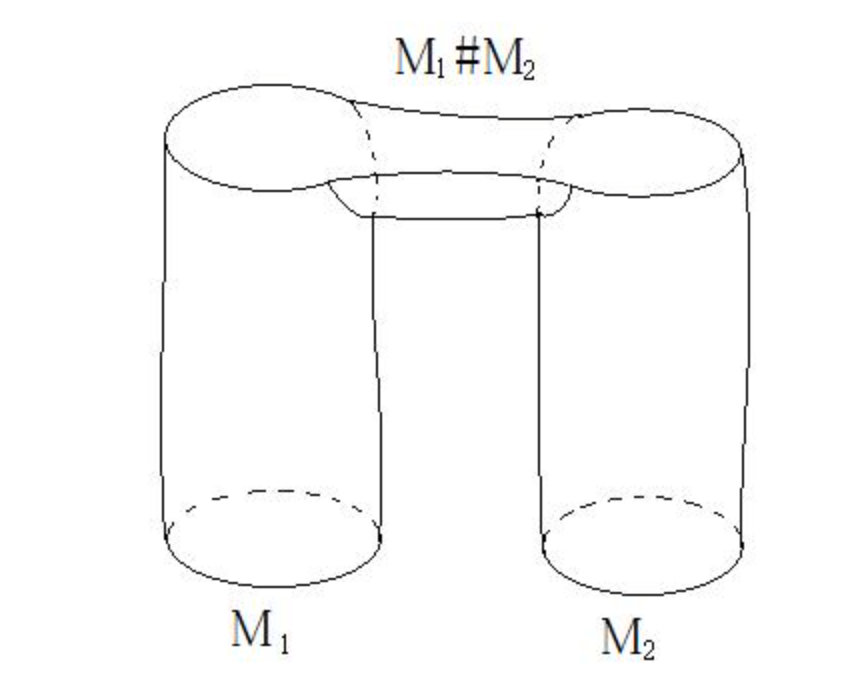
\includegraphics[width=6cm]{images/Lecture 2/Bordism connected sum to disjoint union.png} 
        \caption{\small{The illustration by the \href{http://www.map.mpim-bonn.mpg.de/Bordism\#Connected_sum_and_bordism}{Manifold Atlas Project} of the bordism constructed in the proof above}}
    \end{measuredfigure}
\end{figure}
\end{proof}
%add Drawings inspired by the Prof.'s examples?
\begin{thm}
\label{Cobordant Equiv}
Being cobordant is an equivalence relation on closed $n$-manifolds. 
\end{thm}
\begin{proof}
We need to show that the relation satisfies the properties of reflexivity, symmetry and transitivity:
\begin{itemize}
    \item Reflexive: $Y_0 \sim Y_0$ since we can take $X = Y_0 \times [0,1]$ as in the previous example. We then have $\de X = Y_0 \times \{0,1\} \xrightarrow{p} \{0,1\}$. 
    %
    \item Symmetric: assume $Y_0 \sim Y_1$. Thus, we have $(X,p)$ from $Y_0$ to $Y_1$. We can use the same manifold and compose $p$ with the $swap$ of 0 and 1 in order to get 
    $$\tilde{p}=swap \circ p:\de X\xrightarrow{p}\{0,1\}\xrightarrow{swap}\{1,0\}$$ Consequently, $(X, swap \circ p)$ is a bordism from $Y_1$ to $Y_0$.
    %
    \item Transitive: we have $Y_0 \sim Y_1$ via $(X_1, p_1)$ and $Y_1 \sim Y_2$ via $(X_2, p_2)$. 
    Then we can use as a manifold $X = X_1 \cup_{Y_1} X_2$ where $\cup_{Y_1}$ indicates the gluing along $Y_1$. 
    This is a manifold but there's some work involved in showing it's a \textit{smooth} manifold and it will be done later 
    on (\ref{BordantTransitive}), via an equivalent definition of bordism. We then think of the boundary in the following
     way $\de X = \de_{in} X_1 \amalg \de_{out} X_2$.
\end{itemize}
\end{proof}

\section{Cobordism groups}\label{Cob Groups}
\begin{defn}
\label{Defn n-th cob group}
The set underlying the $n$-th cobordism group is
$$\Omega_n = \frac{\{\text{closed $n$ manifolds}\}}{\{\text{$n+1$ cobordisms}\}}$$
$(\Omega_n, \amalg)$ is an abelian group with operation given by the disjoint union $\amalg$.
	\begin{enumerate}
		\item the disjoint union is associative and commutative
		\item the identity element\footnote{We will
			sometimes write $0=[\emptyset]$ or more often $\emptyset=[\emptyset]$}
			 is the cobordism class of the empty set\footnote{Reminder: $\emptyset$ is an $n$-manifold for every $n$.}
			  $[\emptyset]$, i.e. the set of $n$-manifolds which are bordant with the empty set
		\item every element has an inverse:
		$[M]\amalg [M]=[\emptyset]$ since $M\amalg M=(\de(M\times[0,1]))$ and such a cylinder can be bent into a
		 macaroni, which is bordant to the empty set:
		 \[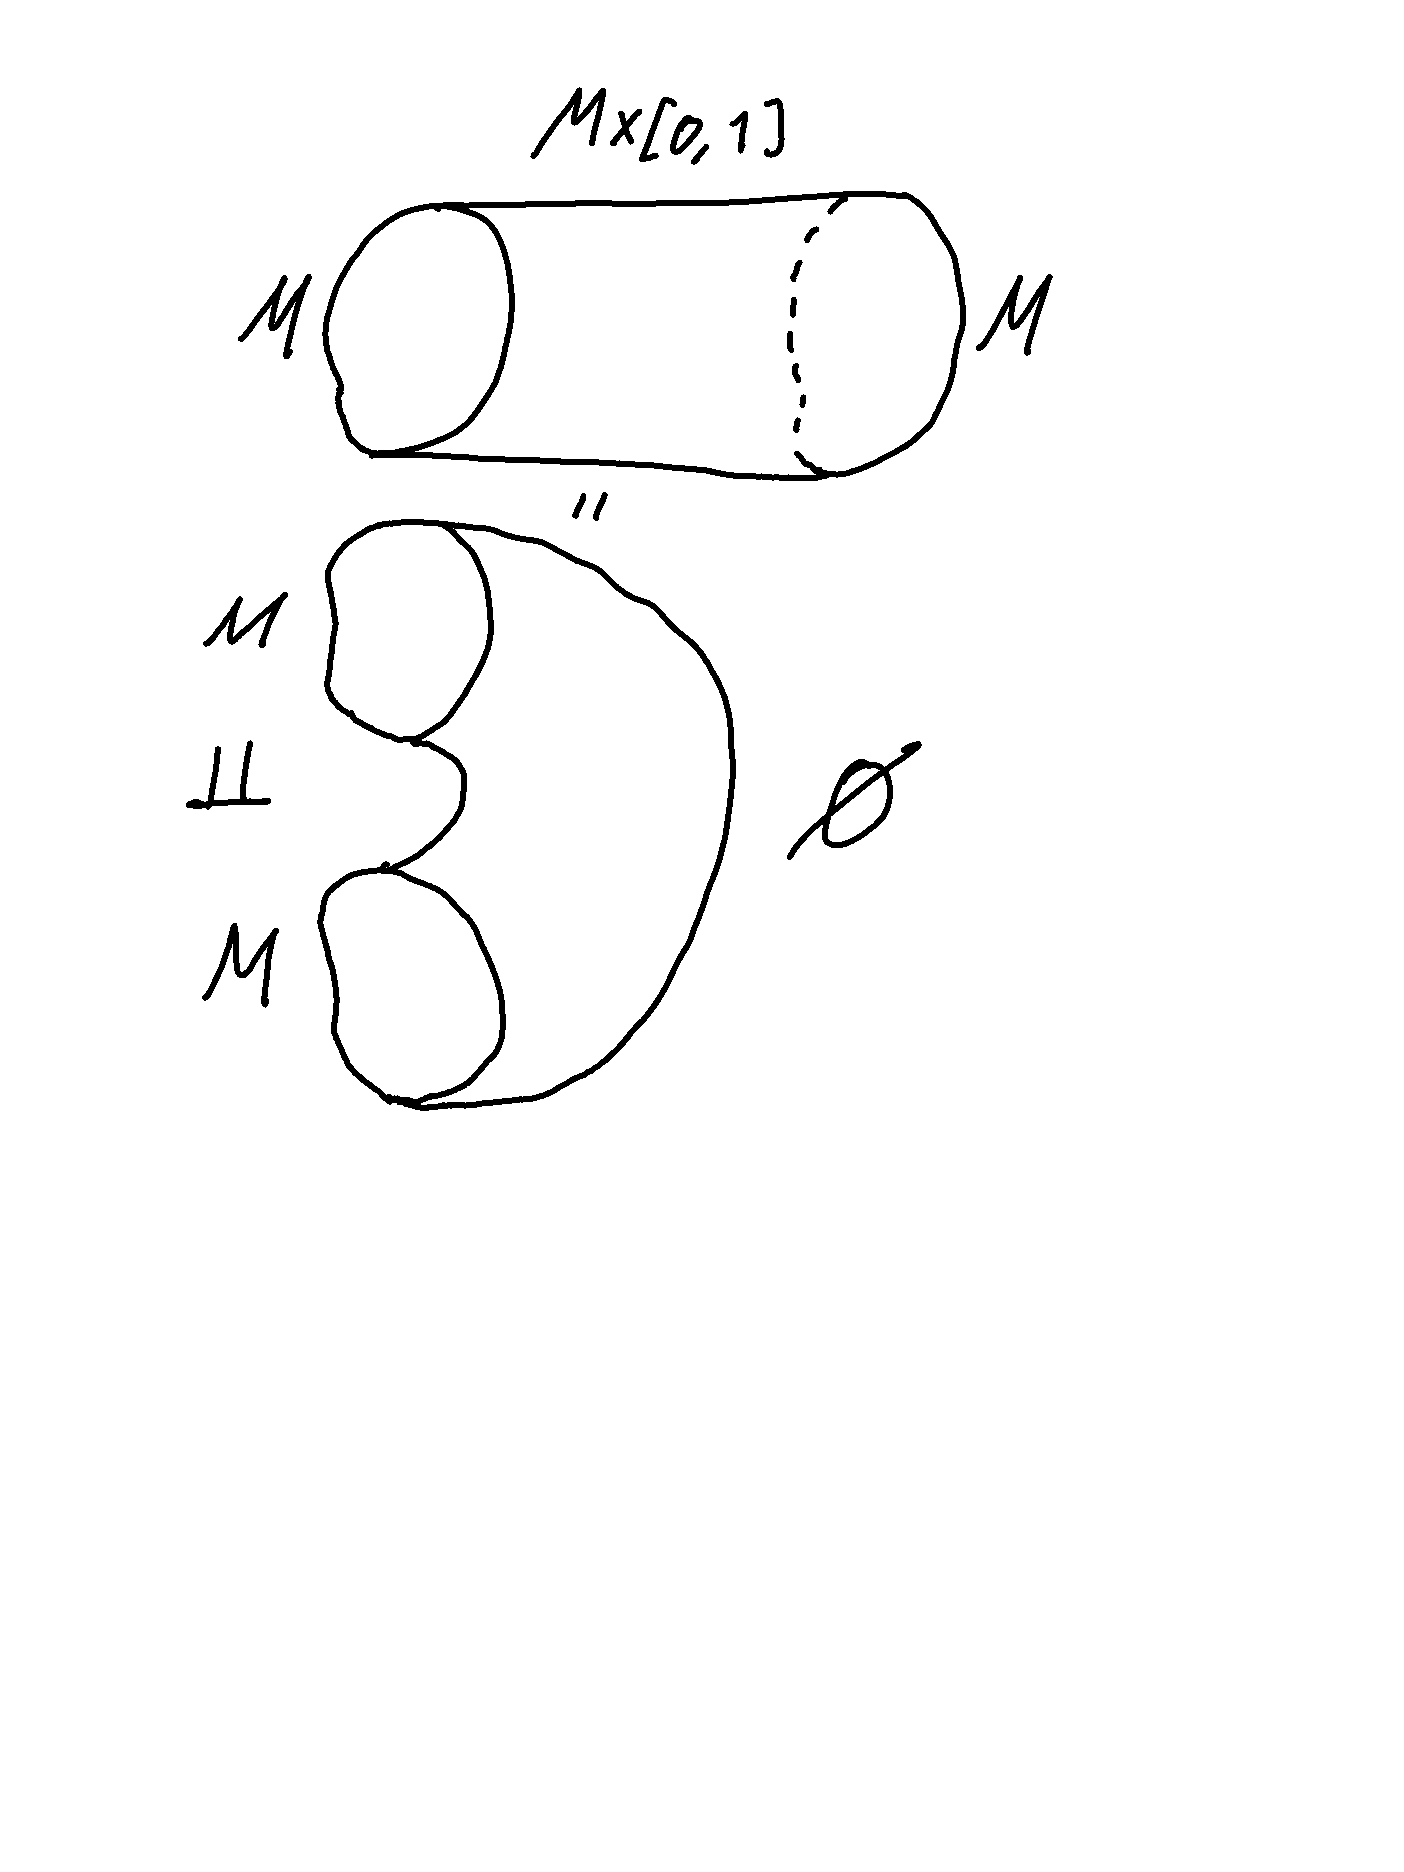
\includegraphics[width=6.5cm]{images/Lecture 2/MACARONI.png}\]
	\end{enumerate}
\end{defn}
\begin{rem}
There is an insidious set-theoretic issue when we define the $n$-th cobordism group $\Omega_n$ (\ref{Defn n-th cob group}): is the collection of all closed $n$ manifolds a set? And what about the collection of all $n+1$ bordisms? It could be the case that it is something bigger than a usual set, thus not a set and problematic since we would not know how to treat them\footnote{We are assuming to be working in ZFC. There are other set theories in which one can define collections greater than sets, e.g. Von Neumann–Bernays–Gödel set theory.}. For example, we know that the collection of all sets is strictly greater than any set\footnote{Because of famous set-theoretic paradoxes like Cantor's paradox.} and thus not a set. Similarly, also the collection of topological spaces is not a set because we can regard any set as a topological space via the discrete topology\footnote{The topology where the set of open sets is the powerset of the set in question, or in other words where any subset is open.}. One could wonder if the collection of all manifolds of a certain dimension $n$ is likewise not a set. This is fortunately for us not the case. The following theorem allows us to happily treat \{\text{closed $n$ manifolds}\} and \{\text{$n+1$ cobordisms}\} as sets by replacing abstract manifolds and cobordism by manifolds and cobordisms embedded in $\R^{\infty}$.
\end{rem}
\begin{thm}[Whitney Embedding theorem\footnote{This result is not important only in this case, but notably for the interest of this class it was used to construct an apt category of bordisms \ref{CobCat} in order to sketch a partial proof of the most important conjecture in the field of TFTs: the cobordism hypothesis; see for details on this \cite{lurie2009classification} and \cite{Calaque_2019}.}]
    Any $n$ manifold can be embedded in $\R^{\infty}(=\bigcup_{n\in\N}\R^n)$. The space of such embeddings is contractible.\footnote{Note that there are refinements of the latter result.}
\end{thm}

\begin{rem}
    Actually $(\Omega_n,\amalg)$ is a finitely generated abelian group, but this is a hard theorem. In particular, it is a finite product of cyclic groups of order $2$ (from 2.)
\end{rem}

\begin{defn}[Bordism invariant]
	A bordism invariant is a homomorphism of abelian groups $$(\Omega_n,\amalg,\emptyset) \to (A,\cdot,e)$$ 
	the abelian group $A$ can be $\Z$, $\R$ or $\C$ for instance.
\end{defn}
\begin{rem}
	Many important manifold invariants are also bordism invariants.
\end{rem}

\begin{ex}
\hfill
\begin{itemize}%TODO complete
    \item $\chi$ mod 2 (the Euler characteristic)
    \item signature
    \item characteristic classes such as Pontrjagin, Stiefel-Whitney or Chern classes 
\end{itemize}
\end{ex}
%TODO add definition of characteristic class or maybe just some additional comment
\subsection{The 0-th Cobordism Group, \texorpdfstring{$\Omega_{0}$}{Omega 0}}
Consider
 $$\Omega_0 = \{\text{finite disjoint unions of points}\} / \{\text{$1$-dimensional cobordisms}\}.$$
To compute this, consider the following classification of $1$ manifolds:

\begin{prop}\label{prop:classification_1d}
Any $1$ dimensional compact manifold with boundary is diffeomorphic to a finite disjoint union of closed intervals $[0,1]$ and circles $S^1$.
\end{prop}
%TODO add proof, it should not be hard, and useful also for classification of 1TFT
\begin{ex}
An example of a $1$-dimensional cobordism is $W=[0,1]$. Here are the 3 different way of seeing it as a bordism: from $Y_0 = \{0,1\}$ to $Y_1 = \emptyset$, from $Y_0 = \{0\}$ to $Y_1 = \{1\}$ and from $Y_0 = \emptyset$ to $Y_1 = \{0,1\}$.
\begin{figure}[H]
    \centering
    \begin{tikzpicture}
        % Line segment
        \draw[line width=1pt] (0,0.5) arc (90:270:-0.5 and 0.5);
  
        % Filled dots at the ends
        \fill (0,0.5) circle (2pt);
        \fill (0,-0.5) circle (2pt);

        \draw[line width=1pt] (3.5,0) -- (4.5,0);
  
        % Filled dots at the ends
        \fill (3.5,0) circle (2pt);
        \fill (4.5,0) circle (2pt);

        \draw[line width=1pt] (8,0.5) arc (90:270:0.5 and 0.5);
  
        % Filled dots at the ends
        \fill (8,0.5) circle (2pt);
        \fill (8,-0.5) circle (2pt);
    \end{tikzpicture}
    %\caption{}
\end{figure}
\end{ex}

\begin{ex} Here is a list of various finite disjoint unions of points with different cardinalities. Can you see a pattern emerging?
\begin{figure}[H]
    \captionsetup[subfigure]{labelformat=empty}
    \centering
    \begin{subfigure}[t]{.3\textwidth}
        \centering
        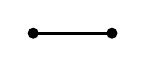
\begin{tikzpicture}
            \draw[line width=1pt] (0,0) -- (1,0);
      
            \fill (0,0) circle (2pt);
            \fill (1,0) circle (2pt);
        \end{tikzpicture}
        \caption{1 point}
    \end{subfigure}
    %
    \begin{subfigure}[t]{.3\textwidth}
        \centering
        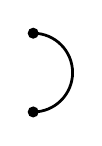
\begin{tikzpicture}
            \draw[line width=1pt] (0,0.5) arc (90:270:-0.5 and 0.5);
      
            \fill (0,0.5) circle (2pt);
            \fill (0,-0.5) circle (2pt);
        \end{tikzpicture}
        \caption{2 points}
    \end{subfigure}
    %
    \begin{subfigure}[t]{.3\textwidth}
        \centering
        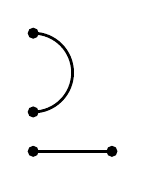
\begin{tikzpicture}
            \draw[line width=1pt] (0,0.5) arc (90:270:-0.5 and 0.5);
      
            \fill (0,0.5) circle (2pt);
            \fill (0,-0.5) circle (2pt);
    
            \draw[line width=1pt] (0,-1) -- (1,-1);
      
            \fill (0,-1) circle (2pt);
            \fill (1,-1) circle (2pt);
        \end{tikzpicture}
        \caption{3 points}
    \end{subfigure}

    \bigskip
    
    \begin{subfigure}[t]{.3\textwidth}
        \centering
        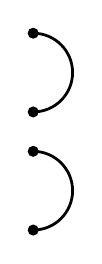
\begin{tikzpicture}
            % Line segment
            \draw[line width=1pt] (0,0.5) arc (90:270:-0.5 and 0.5);
      
            % Filled dots at the ends
            \fill (0,0.5) circle (2pt);
            \fill (0,-0.5) circle (2pt);

            % Line segment
            \draw[line width=1pt] (0,-1) arc (90:270:-0.5 and 0.5);
      
            % Filled dots at the ends
            \fill (0,-1) circle (2pt);
            \fill (0,-2) circle (2pt);
        \end{tikzpicture}
        \caption{4 points}
    \end{subfigure}
    %
    \begin{subfigure}[t]{.3\textwidth}
        \centering
        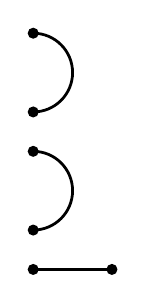
\begin{tikzpicture}
            % Line segment
            \draw[line width=1pt] (0,0.5) arc (90:270:-0.5 and 0.5);
      
            % Filled dots at the ends
            \fill (0,0.5) circle (2pt);
            \fill (0,-0.5) circle (2pt);

            % Line segment
            \draw[line width=1pt] (0,-1) arc (90:270:-0.5 and 0.5);
      
            % Filled dots at the ends
            \fill (0,-1) circle (2pt);
            \fill (0,-2) circle (2pt);

            % Line segment
            \draw[line width=1pt] (0,-2.5) -- (1,-2.5);
      
            % Filled dots at the ends
            \fill (0,-2.5) circle (2pt);
            \fill (1,-2.5) circle (2pt);
        \end{tikzpicture}
        \caption{5 points}
    \end{subfigure}
    %
    \begin{subfigure}[t]{.3\textwidth}
        \centering
        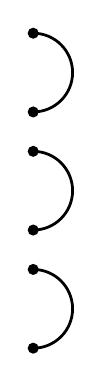
\begin{tikzpicture}
            % Line segment
            \draw[line width=1pt] (0,0.5) arc (90:270:-0.5 and 0.5);
      
            % Filled dots at the ends
            \fill (0,0.5) circle (2pt);
            \fill (0,-0.5) circle (2pt);

            % Line segment
            \draw[line width=1pt] (0,-1) arc (90:270:-0.5 and 0.5);
      
            % Filled dots at the ends
            \fill (0,-1) circle (2pt);
            \fill (0,-2) circle (2pt);

            % Line segment
            \draw[line width=1pt] (0,-2.5) arc (90:270:-0.5 and 0.5);
      
            % Filled dots at the ends
            \fill (0,-2.5) circle (2pt);
            \fill (0,-3.5) circle (2pt);
        \end{tikzpicture}
        \caption{6 points}
    \end{subfigure}
\end{figure}
\end{ex}

\noindent Keeping this pattern in mind, consider collection of $k$ points, with $k$ finite (i.e. the only closed 0 manifolds):

\begin{itemize}
	\item If $k$ is even, we can find a bordism to $\emptyset$
	\item If $k$ is odd, we can find a bordism to $\{*\}$
\end{itemize}

\noindent We then have 
\begin{equation*}
    2k \text{ points} \sim \emptyset, \quad\quad 2k+1 \text{ points} \sim \text{1 point}
\end{equation*}
Therefore, the 0-th cobordism group is given by
\begin{equation}
    \Omega_0 = \{ \emptyset, \{*\}\} \cong \Z_2.
\end{equation}
A possible variation is: add a ``decoration'', called \textit{orientation} (will be made more precise later), so we now have:
$$\Omega_0^{\textit{or}} = \big\{\text{finite sets of points $S$ with a map } S \to \{+,-\}\big\} /\{\text{oriented cobordism}\}$$

An oriented cobordism in $1$ dimension is given by $[0,1]$ or $S^1$ which comes with an orientation. Here are some
examples

\[ 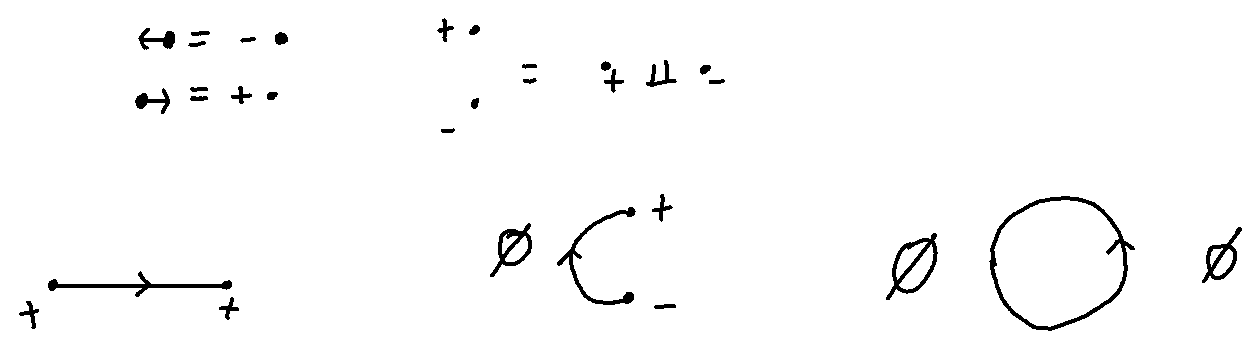
\includegraphics[width=9cm]{images/Lecture 11/1dBORDISM.png}\]

\begin{exercise}
    What is $\Omega_0^{or}$? Try to think about it! 
\end{exercise}

\subsection{The 1st cobordism group, \texorpdfstring{$\Omega_{1}$}{Omega 1}}
Now we have
$$\Omega_1= \{\text{closed $1$-dimensional manifolds}\} / \{\text{$2$-dimensional cobordisms}\}.$$
In studying this group, the following result, which is a restriction of \ref{prop:classification_1d}:
\begin{thm}
    Any closed $1$-dimensional manifold is a finite disjoint union of circles
\end{thm}
\noindent However, a circle is the boundary of a 2-disk, which gives a cobordism from $S^1$ to $\emptyset$, we then have $S^1 \sim \emptyset$. Hence, also finite disjoint unions of $S^1$ are cobordant to the empty set. Therefore, the $1$st cobordism group is trivial:
\begin{equation}
    \Omega_1 = 0
\end{equation}

\subsection{The 2nd cobordism group, \texorpdfstring{$\Omega_{2}$}{Omega 2}}
In order to find the $2$nd cobordism group, we first need a classification of $2$ manifolds. %(Introduced before) In order to state the result we need to introduce the concept of \textit{connected sum}
%\begin{defn}[Connected Sum]
	%Given $n$ manifolds $M,N$, their connected sum $M\# N$ is given by
	%%M\# N = M \setminus (D^n)^\circ \cup_{\de D^n \times [0,1]} N \setminus (D^n)^\circ
	%\end{equation}
%\end{defn}
%DRAWING
\begin{prop}[Classification of $2$-dimensional manifolds]\label{Classification of 2 manifolds}
Every connected closed $2$ manifold is diffeomorphic to
\begin{enumerate}
    \item $S^2$, orientable
    \begin{figure}[!ht]
        \centering
        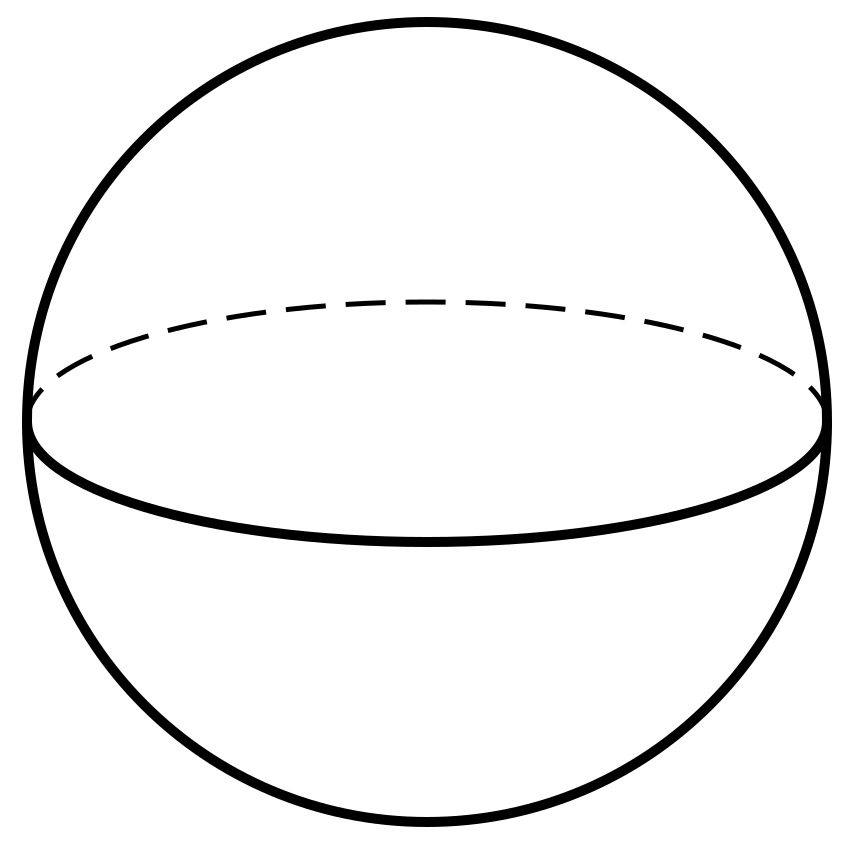
\includegraphics[width=3cm]{images/Lecture 3/sphere.png}
        \caption{2-sphere, $S^2$}
    \end{figure}
    \item $\Sigma_g = \underbrace{T \# \dots \# T}_{g-\text{times}}$ , orientable
    \begin{figure}[!ht]
        \centering
        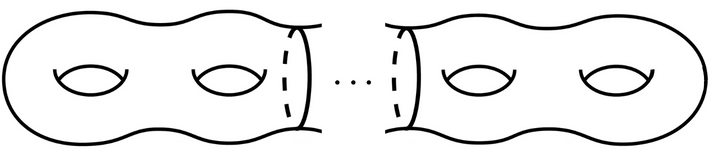
\includegraphics[width=10cm]{images/Lecture 3/surface_of_genus_g.png}
        \caption{Surface of genus g, $\Sigma_g$}
    \end{figure}
    \item $P_k = \underbrace{\R\P^2 \# \dots \# \R\P^2}_{k-\text{times}}$ , non-orientable
    \begin{figure}[!ht]
        \centering
        \begin{subfigure}[t]{.4\textwidth}
            \centering
            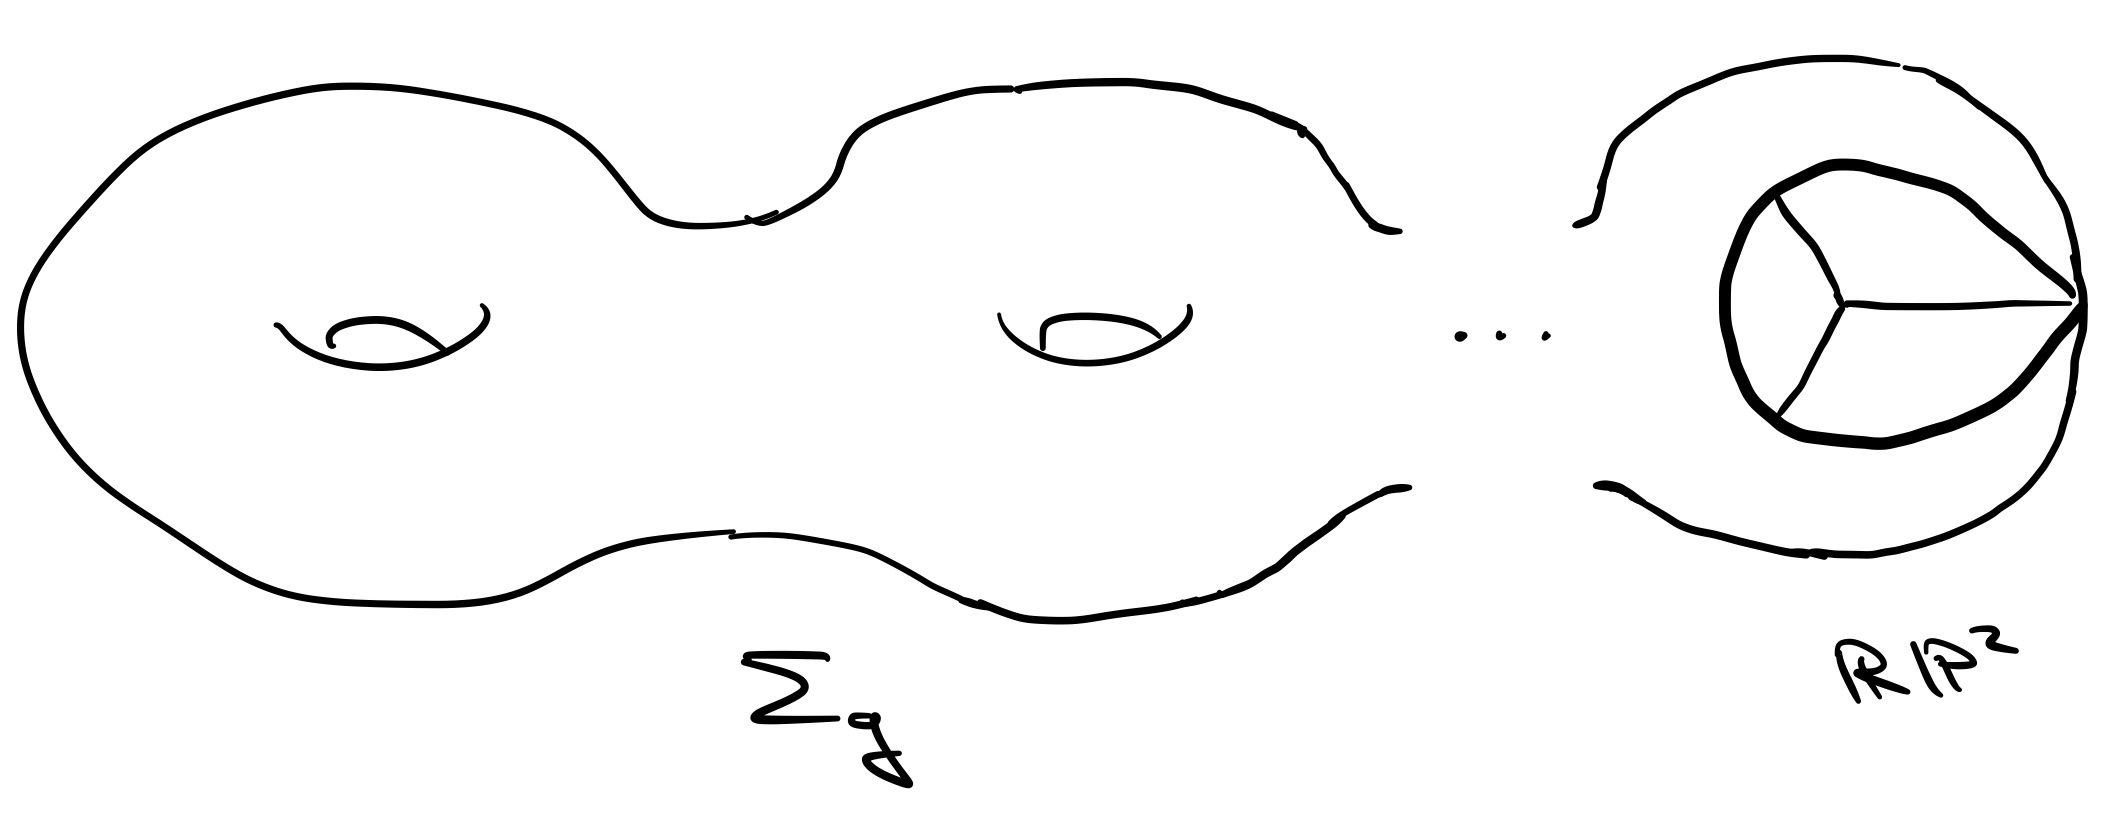
\includegraphics[width=6cm]{images/Lecture 3/sigma_g_rp2.png}
            \caption{$P_{2g+1} \cong \Sigma_g \# \R\P^2$}
        \end{subfigure}\hspace{10mm}
        \begin{subfigure}[t]{.4\textwidth}
            \centering
            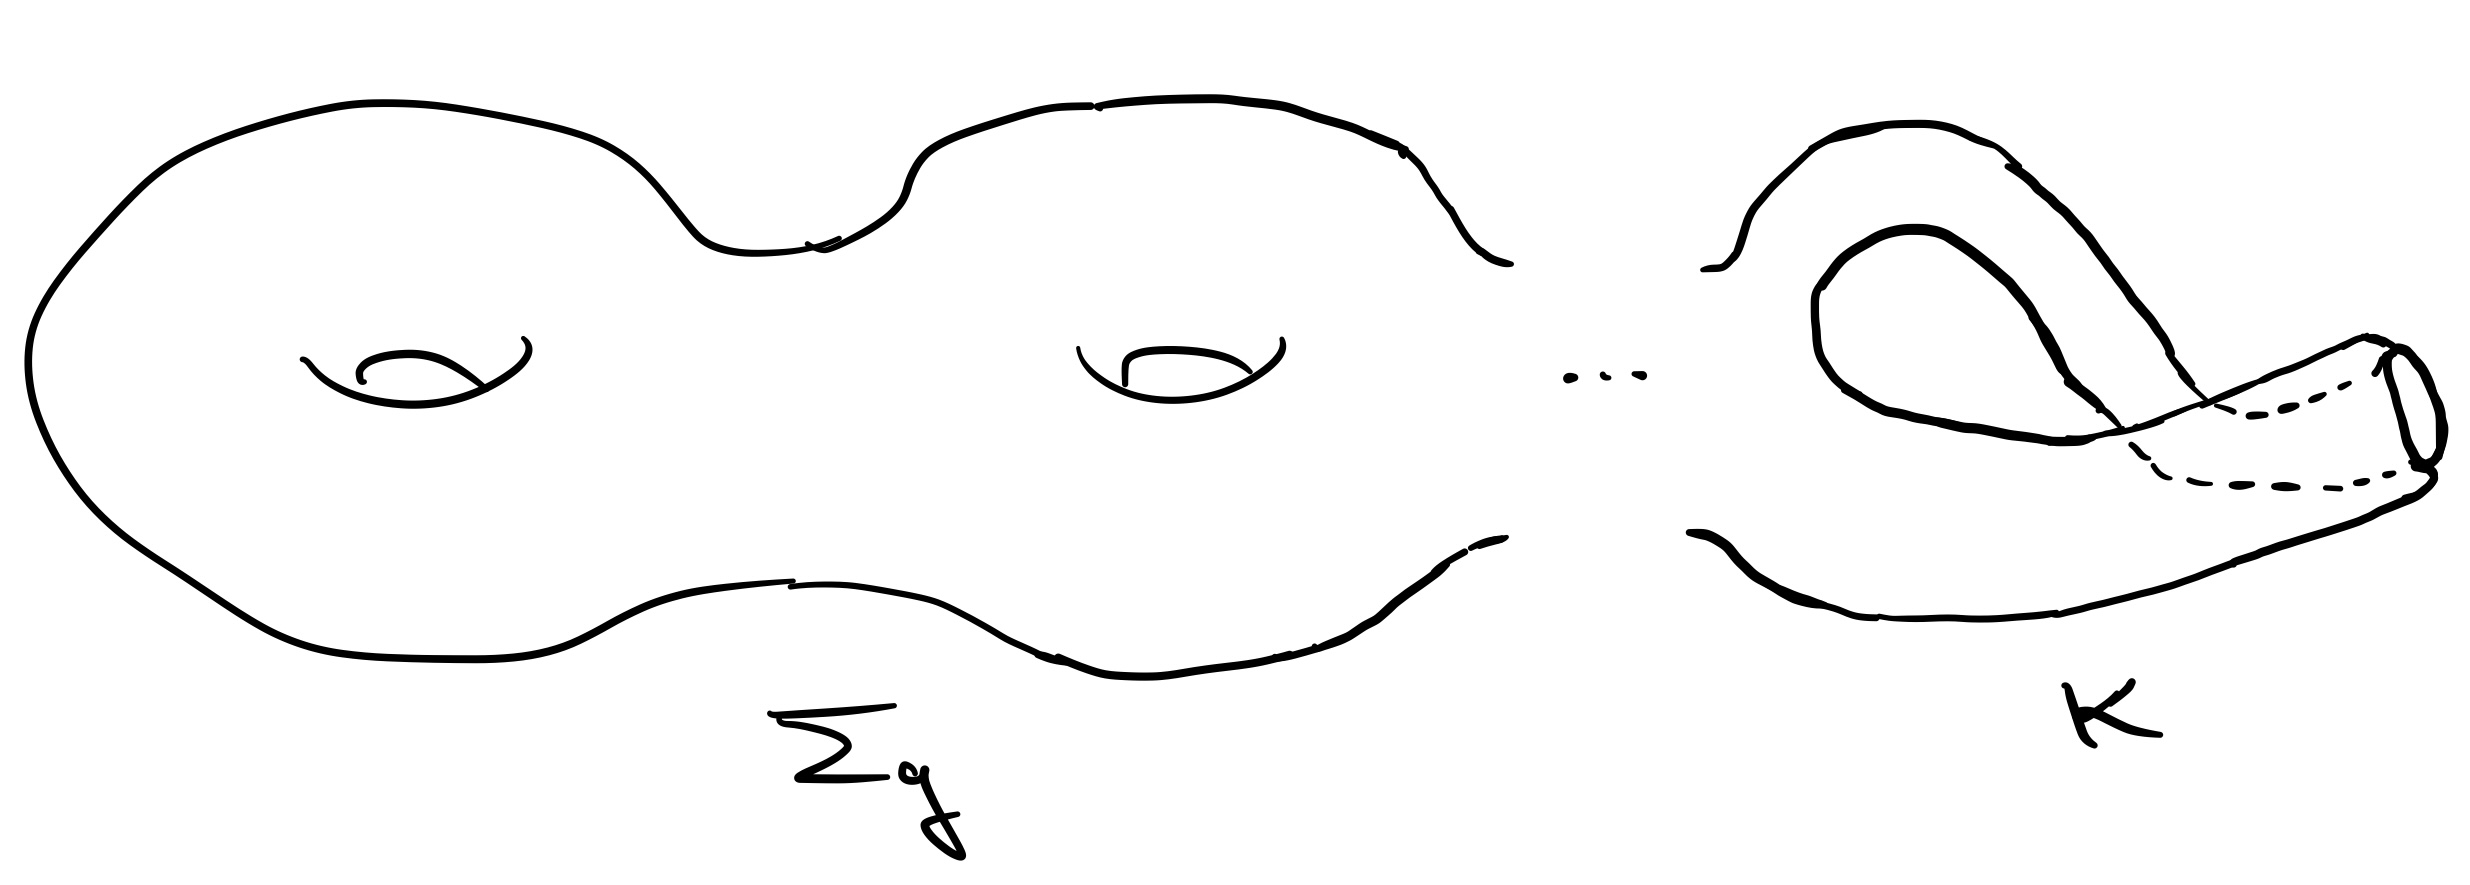
\includegraphics[width=6cm]{images/Lecture 3/sigma_g_klein_bottle.png}
            \caption{$P_{2g+2} \cong \Sigma_g \# K$}
        \end{subfigure}
    \end{figure}
\end{enumerate}
\end{prop}

\noindent We can now use this knowledge to compute
$$
	\Omega_2^{\text{or}} = \{\text{closed oriented $2$ manifolds} \} /\{\text{$3$-dimensional oriented cobordisms}\}
$$
by observing that $S^2$ and $\Sigma_g$ are both cobordant to $\emptyset$ since they can simply be ``filled'' to a $3$ dimensional manifold with boundary, we get
\begin{equation}
    \Omega_2^{or} = 0.
\end{equation} 
%DRAWING
\begin{exercise}
    What about the non-oriented part $\Omega_2$?
\end{exercise}


% -------------------------------------------------------------
% --------------------- LECTURE 3 30/10 -----------------------
% -------------------------------------------------------------
\section{Different definitions of bordisms} % (fold)
\label{sec:different_definitions_of_bordisms}

\begin{rmnd}[Definition \ref{Define Bordism} of Bordism]
Let $Y_0, Y_1$ be closed $n$ manifolds. A bordism $(X,p)$ from $Y_0$ to $Y_1$ consists of a compact $n+1$ manifold with boundary together with a map $p: \de X \to \{0,1\}$ such that $Y_0 \text{\colorbox{yellow}{=}} p^{-1}(0)$ and $Y_1 \text{\colorbox{yellow}{=}} p^{-1}(1)$ (hence $\de X \text{\colorbox{yellow}{=}}  Y_0 \amalg Y_1$). We say that $Y_0$ and $Y_1$ are \textit{cobordant}.
\end{rmnd}

\noindent There was a complaint: why don't we use diffeomorphisms instead of the highlighted equalities? This question arises because even with simple examples the equality seems too strict:

\begin{rmnd}[from \ref{Cobordant Equiv}]
Being cobordant is an equivalence relation.
\end{rmnd} 

\noindent In particular, for any closed $n$ manifold $Y$ we have $Y\sim Y$. The bordism is given by the cylinder $Y\times [0,1]$, where $p:Y\times\{0,1\}\to \{0,1\}$. Then $Y\times\{0\}=p^{-1}(0)$, but $Y\neq Y\times\{0\}$! 
It seems like our previous definition does not actually give rise to an equivalence relation. 
%TODO is this above what we wanted to say? /William
Instead, if we substitute the strict equalities with diffeomorphisms (isomorphisms in the category of smooth manifolds) things seem to work out flawlessly:

\begin{defn}[$2^{nd}$ variant of the definition of bordism: via diffeomorphisms]
\label{NewDefBord}
    Let $Y_0, Y_1$ be closed $n$ manifolds. A bordism from $Y_0$ to $Y_1$ is a quadruple $(X,p,\phi_{0},\phi_{1})$ consisting of a compact $n+1$ manifold with boundary $\de X$ together with maps 
    \begin{align*}
        p&: \de X \to \{0,1\}        \\
        \phi_{0}&:Y_{0}\xrightarrow{\cong} p^{-1}(0) \\
        \phi_{1}&:Y_{1}\xrightarrow{\cong} p^{-1}(1)
    \end{align*}
    (we therefore have $\de X \cong Y_0 \amalg Y_1$).
\end{defn}

\begin{ex}
    Let $\psi:M\xrightarrow{\cong} N$ be a diffeomorphism.
    Then $(M\times [0,1], M\times\{0,1\}\xrightarrow{p}\{0,1\}, \phi_0, \phi_1)$, with maps
    $$\phi_0:M\xrightarrow{id\times\{0\}}p^{-1}(0)=M\times \{0\}$$
    $$\phi_1:N\xrightarrow{\psi^{-1}\times\{1\}}p^{-1}(1)=M\times\{1\}$$
    gives a bordism from $M$ to $N$.
    This is called the mapping cylinder of $\psi$. 
    
    \noindent$\Rightarrow$ under the new definition, \underbar{any} two diffeomorphic manifolds are also cobordant.
\end{ex}

%TODO it's not really clear what the mapping cylinder is

Why does this not change the definition of bordism?
Because any diffeomorphism also gives a bordism in the old sense:
Given $M\xrightarrow{\cong}N$, take the gluing $(M\times I)\underset{M\times\{1\}}{\coprod_{\psi}}N$ so that $Y_1=N$ and $Y_0=M\times \{0\}"="M$ (abusing notation).

\noindent Now we prove the transitivity of the relation 'being cobordant'. We do that by showing that given $X$ from $Y_0$ to $Y_1$ and $X'$ from $Y_1$ to $Y_2$, we can glue them along the boundary in common, $Y_1$, to obtain a bordism from $Y_0$ to $Y_2$. %add diagram here (?) later works as well
In order to achieve this, we need to introduce the following notion:
\begin{defn}[Collar of a boundary]
    Let $X$ be a manifold with boundary. A collar of the boundary is an open set  $U\subseteq X$ containing $\de X$ together with a diffeomorphism  $(-\epsilon,0]\times\partial M \to U$ for some $\epsilon>0$.
\end{defn}
\begin{thm}
	The boundary of a manifold with boundary always has a collar.
\end{thm}
\begin{proof}[Idea of the proof]
    We start with a manifold with boundary, locally at $x\in\de X$ we have 
    $$(-\epsilon_x, 0]\times V_x\xrightarrow{\cong} U_x\subseteq\mathbb{H}^n$$
    where $V_x$ is an open neighbourhood of $x$ in $\de X$.
    \noindent Now we use a standard trick in differential geometry/topology (see \cite{Hirsch1976}): globally patch these diffemorphisms using a partition of unity. It works if $X$ is compact.
\end{proof}

\begin{defn}[$3^{rd}$ variant of the definition of bordism: via collars]
    Let $Y_0$ and $Y_1$ be closed $n$ manifolds. A bordism from $Y_0$ to $Y_1$ is a quadruple $(M, p, \phi_0, \phi_1)$ with $M$ and $p$ as before. $\phi_0, \phi_1$ are given by
    $$\phi_0:[0, \epsilon)\times Y_0\to U \supseteq p^{-1}(0)$$
    $$\phi_1:(-\epsilon, 0]\times Y_1\to V \supseteq p^{-1}(1)$$
    where $U$ and $V$ together form a collar of the boundary of $M$.
\end{defn}

\noindent Moreover, 
$$([0, \epsilon)\times Y_0\big)\amalg((-\epsilon, 0]\times Y_1)\xrightarrow{\phi_0\amalg\phi_1}
\big(U\amalg V\big)\supseteq 
\Big(p^{-1}(0)\amalg p^{-1}(1)\Big)=\de M$$
%TODO what is this for?

\noindent This variant of the definition is equivalent to the other two but we would unfortunately need a lot of differential topology in order to prove this.

However, with the third definition we can finally prove the following claim which then is what we were missing to prove transitivity of being cobordant.
\begin{clm}\label{GluedManifoldsBordisms}
    $X\underset{Y_1}{\cup} X'$ admits a smooth structure.
\end{clm}
\begin{proof}[Transitivity of cobordant]\label{BordantTransitive}
    We need a maximal atlas with smooth transition functions. Clearly, in the interior points of $X$ and $X'$ this exists since we can use directly the charts of $X$ and $X'$. The problem is the double collar around $Y_1$. So we need to construct charts around points on $Y_1$. Take $U_1^{-}\underset{Y_1}{\cup}U_1^{+}$ in an open neigbourhood. Then via $U_1^{-}\underset{Y_1}{\cup}U_1^{+}\xrightarrow{\phi_1\cup\phi'_0}(-\epsilon,\epsilon)\times Y_0=(-\epsilon,0]\cup[0,\epsilon)\times Y_0$ which contains $(-\epsilon,\epsilon)\times V_x$ which maps to $\R^n$ via $\psi_x$ and thereby generating a maximal atlas.

%TODO not very clear
Let $X$ be a bordism between $Y_0$ to $Y_1$ and $X'$ between $Y_1$ and $Y_0$.
%drawings
$$[0, \epsilon)\times Y_0\xrightarrow{\phi_0}U$$
$$(-\epsilon,0]\times Y_1\xrightarrow{\phi_1}U_1^{-}$$
$$[0,\epsilon)\times Y_1\xrightarrow{\cong}(-\epsilon,0]\times Y_1\xrightarrow{\phi'_0}U_1^{+}$$
$$(-\epsilon,0]\times Y_2\xrightarrow{\phi'_1}U_2$$
\end{proof}

\section{Tangential Structures}
\subsection{Orientations and the tangent bundle}
\begin{defn}[Tangent bundle]
    The tangent bundle $TM$ of a bundle $M$ is the vector bundle over $M$ of rank $n$ with
    \begin{enumerate}
        \item fibers given by the tangent spaces $T_p M$ at each point $p \in M$: $$(TM)_p=T_pM$$
        \item (as a set) $TM=\coprod_{p\in M} T_p M$ with natural projection: 
        \begin{align}
        	TM=\coprod_{p\in M} T_p M&\xrightarrow{p}M \\
        	(p,v)&\mapsto p
        \end{align}
    \end{enumerate}
\end{defn}

\noindent It is possible to define a topology on $TM$ such that it is a smooth $2n$ manifold: $(U,\phi)$ chart of $M$, we have a chart of $TM$, $(p^{-1}(U),\tilde\phi)$ by looking at preimages of $U$ under the projection map and we construct the local trivialization with the usual construction. 
%TODO maybe say a bit more about local trivialisations
This is summarized by the fact that the following diagram commutes:
\[\begin{tikzcd}
	{p^{-1}(U)=TU=\coprod_{p\in U}T_pM} && {T\tilde U=\tilde U\times\R^n} \\
	\\
	U && {\tilde U\subseteq\R^n}
	\arrow["p", from=1-1, to=3-1]
	\arrow["{\tilde\phi=(\phi,d\phi)}"', from=1-1, to=1-3]
	\arrow["pr_{\tilde U}", from=1-3, to=3-3]
	\arrow["\phi"', from=3-1, to=3-3]
	\arrow["\cong", from=3-1, to=3-3]
\end{tikzcd}\]
This is actually an atlas with smooth structure. Transition functions $g_{ij} = \tilde \phi_j \circ \tilde\phi_i^{-1}|_{\tilde \phi_i(U_i \cap U_j)}$ are actually the jacobian and we have $g_{ij} \in GL_n(\R)$. 

\begin{defn}[Orientability and admissibility of $G$ structure]
    If $TM$ has local trivializations such that the transition functions between overlapping trivializations are in $ GL_n^+(\R)\subseteq GL_n(\R)$ then we say that $M$ is orientable.

    \noindent In other words "The structure group of $TM$ can be reduced to $GL_n^+ (\R) \subset GL_n(\R)$".
    
    \noindent Analogously, given some $G \subset GL_n(\R)$, we can say $M$ admits a $G$ structure if the local trivialisations are such that $\phi_{i,j} \in G$, i.e. "the structure group can be reduced to $G$". In this sense, being orientable is the same as admitting a $GL_n^+ (\R)$ structure.

\end{defn}

% -------------------------------------------------------------
% --------------------- LECTURE 4 6/11 -----------------------
% -------------------------------------------------------------

\begin{ex}
\hfill
	\begin{itemize}
		\item $\R^n$: we have $T\R^n \cong \R^n \times \R^n$, meaning the tangent bundle is a trivial bundle.
		\item $S^1$: we again have the trivial bundle $TS^1 \cong S^1 \times \R$
		\item $S^2$: now $TS^2 \ncong S^2 \times \R^2$, it is not a trivial bundle. This follows from the \href{https://en.wikipedia.org/wiki/Hairy_ball_theorem}{hairy ball theorem}. 
	\end{itemize}
	All these are orientable. Instead examples of non orientable manifolds are the Klein bottle, the Möbius strip and $\R\P^2$.
 %drawings 
\end{ex}

\begin{defn}[Orientation and $G$ structure]
    An orientation (equivalently, a $GL^+_n(\R)$ structure) of $M$ is an equivalence class of trivialisations $\{(\tilde U, \tilde \phi)\}$ of $TM$ such that $\det g_{ij} > 0$ (i.e. $g_{ij} \in GL^+(n,\R)$).

    \noindent Analogously, given some $G \subset GL_n(\R)$, a $G$ structure on $TM$ is an equivalence class of trivialisations $\{(\tilde U, \tilde \phi)\}$ such that $g_{ij} \in G$.
\end{defn}

\noindent We can now note the following lemma which is related to the fact that on a manifold one can always construct a Riemannian metric.
\begin{lem}
	A $GL_n^+ (\R)$ structure is the same as an $SO(n)$ structure.
\end{lem}

\noindent How many orientations can $M$ have? 0 if it's not orientable, 2 if it's connected and orientable, in general $2^{\# \text{ connected components}}$ if it's orientable.

\begin{defn}[Opposite orientation]
	$M$ oriented with charts $\{(U_i, \phi_i)\}$. The opposite orientation on $M$ is given by: $\{(U_i, \bar \phi_i)\}$ in which $\bar \phi_i$ is given by the following composition
	\begin{equation}
		U_i \xrightarrow{\phi_i} \R^n \to \R^n %TODO write better
	\end{equation}
	We will indicate $M$ with opposite orientation by $\bbar M$.
\end{defn}

\begin{ex}
	$S^1$ %DRAWING
\end{ex}

\begin{defn}[Orientation preserving and reversing diffeomorphism]
	A diffeomorphism $\psi: M \to N$ between oriented manifolds is orientation preserving (reversing) if the orientation on $N$ induced by the one on $M$ is the (opposite) orientation on $N$.
\end{defn}
\begin{ex}
	Consider maps $S^1 \to S^1$ (implicitly using the same orientation on each $S^1$). The identity is an orientation preserving map, while the map $x \mapsto \bar x$ is orientation reversing (considering $S^1 \subset \C$).

	\noindent We could instead consider maps $S^1 \to \bbar{S^1}$. In this case the identity is orientation reversing.
\end{ex}

Given a manifold $M$ with boundary, its tangent bundle (how is it defined?) contains a copy of $T(\de M)$.
%DRAWING
This is because we can "glue another collar" $[0,\epsilon]$ onto the boundary so that the points that were on the boundary are now interior points. This allows us to define $T_x M$ for $x \in \de M$, the tangent bundle for boundary points. Instead, considering $\de M$ as its own manifold we have $T_x \de M$ and we have that $T_x \de M \subset T_x M$ and it has codimension 1. We can then define the quotient
$$
	\nu_x = T_x M /T_x \de M
$$
and we can write the following short exact sequence of bundles on $\de M$.
\begin{equation}
	0 \to T(\de M) \to i^* TM \to \nu \to 0
\end{equation}
in which $i: \de M \to M$ is the inclusion and $i^*: TM$ (bundle over $M$) $\to TM$ (bundle over $\de M$) is its pullback. 
%TODO did I understand this correctly?
If we fix a local chart with coordinates $x_1, \dots, x_n$ we have a basis $\frac{\de}{\de x_1}$ for $\nu$.

\noindent This has the following consequences:
\begin{enumerate}
	\item an orientation on $M$ induces one on $\de M$
	\item $\nu$ has two "orientations" ($\cong$ normal directions)
	\item an orientation on $\de M$ induces one on $\de M \times (0,1)$ (if I choose an orientation on $(0,1)$) but in general we can't extend this construction to all of $M$.

	\noindent More generally, note that if $M$ and $N$ are oriented, then $M\times N$ is oriented. \cite{FreedBordism}
\end{enumerate}

\noindent Special case: 0 dimensional manifold. $M = \{x_1, \dots, x_k\}$, but $T_x M = 0$ so our definition fails! So in this case the definition does not capture what we would like, in particular the consequences we found before are either tautological or boring. We can however use 3. to construct a new definition.
\begin{defn}
	An orientation on a 0 dimensional manifold is a map $M \to \{\pm 1\}$ ($\iff$ orientation of $M \times (0,1)$ if I fixed a chosen orientation of (0,1)).
%don't understand why have to fix an orientation of the interval /William
	%DRAWING
\end{defn}

\begin{defn}[Oriented bordism]
	Let  $Y_0$ and $Y_1$ be oriented closed $n$ manifolds.
	An oriented bordism from $Y_0$ to $Y_1$ is an oriented $n+1$ manifold $X$ together with $p: \de X \to \{0,1\}$ and $\psi: \de X \to \bbar Y_0 \amalg Y_1$ an orientation preserving diffeomorphism.
	(Note: now $p$ is actually too much data $\dots$, since it basically tells us which of the $Y_i$ we're reversing, so we can get rid of it.)
	%TODO make this comment clearer
\end{defn}
\noindent Again this is an equivalence relation which we call "being oriented cobordant", which allows us to give the following definition.
\begin{defn}
	The oriented bordism group is:
	\begin{equation}
		\Omega_n^{or} = \{\text{closed oriented $n$ manifolds}\}/\{\text{oriented $n+1$ cobordisms}\}
	\end{equation}
\end{defn}
\begin{rem}
	Note that $\emptyset$ is an oriented $n$ manifold with a unique orientation.
\end{rem}

\subsection{Framings} % (fold) 
\label{sub:framings}

Recall the definition of a $G$ structure given above. As stated previously, if $G = GL_n^+(\R)$ a $G$ structure is an orientation. Another choice is simply to take $G = \{e\}$, this gives a \textit{framing}, which amounts to a smooth choice of basis for every point. We can talk about \textit{frameable} or \textit{parallelizable} manifolds, meaning they admit a framing. As a consequence, the manifold has a trivial tangent bundle we have $TM \cong M \times \R^n$ and a choice of framing corresponds to a choice of isomorphism.

\begin{ex}
Some examples of frameable manifolds are the following:
    \begin{itemize}
        \item For $\R^n$, we have $T\R^n \cong \R^n \times \R^n$
        \item $S^1$
        \item $S^1 \times S^1$
        %choose how many times I rotate when following the circles --> framing
        \item Any Lie group $H$ has $TH \cong H \times \R^{\dim}$
    	\item What about $S^2$? Not frameable because of the hairy ball theorem (we would need two vector fields that are a basis at each point of $S^2$ but because of the theorem we don't even have one).
    \end{itemize}
        %Well for any point $p \in S^1$ we have $T_p S^1 \cong \R$ and the isomorphism is given by a choice of vector. 
\end{ex}

\noindent In fact, there aren't many closed connected 2 manifolds with framing:
\begin{fct}
	The only closed connected 2 manifolds with framing is the torus.
\end{fct}
\noindent This follows from the \href{https://en.wikipedia.org/wiki/Poincar%C3%A9%E2%80%93Hopf_theorem}{Poincaré–Hopf index theorem}\footnote{This differential topology theorem relates the index of a vector field to the Euler characteristic of the manifold. In particular, it implies that a nonvanishing vector field can only exist if the Euler characteristic of the manifold is zero.}.

\begin{lem}
	Any framing on an $n$ manifold $M$ induces an orientation on $M$.
\end{lem}
\noindent From our definition this is immediate because $\{e\} \subseteq GL_n^+$ (however there are other definitions of orientation for which it's not immediate).
%.... induces top form on M


% -------------------------------------------------------------
% --------------------- LECTURE 5 6/11 ------------------------
% -------------------------------------------------------------

\section{Classification of 2 manifolds with boundary} % (fold) // what do you mean by '(fold)'? /andrea
\label{sub:classification_of_2_manifolds_with_boundary}

The aim of this chapter is to prove the aforementioned classification of compact 2-dimensional manifolds with the use of Morse theory (see \ref{Classification of 2 manifolds}). We remind the reader: let $M$ be a 2 manifold with genus $g$, then \begin{itemize}
    \item if $M$ is oriented, $M$ is classified by its genus $g$. In particular $M$ it is diffeomorphic to $\Sigma_g:=T\,\# \dots\#\,T$, the connected sum of $g$-tori, where in particular $\Sigma_0=S^2$.
    \item Instead if $M$ is non orientable\footnote{see \url{https://en.wikipedia.org/wiki/Genus_(mathematics)} for what is meant by genus of a non orientable surface}, $M$ is diffeomorphic to $g$ copies of the real projective plane, i.e.  $\R P^2\,\# \dots \#\,\R P^2$.
\end{itemize} 

One can find a thorough covering of this result in \cite{Hirsch1976}.

\noindent In addition, we will also find a classification of compact 2 manifolds with boundary (which we will simply call \textit{surfaces}). To do it we will need Morse theory. What is the idea? Given a surface $M$ (it works in greater generality but now we're only interested in surfaces), find a map $f: M \to \R$ which is "nice" is a way we'll specify later on.
Then by analizing properties of $f$ we can recover the topology of the surface (i.e. the surface up to diffeomorphism). 

\noindent This section is based on \cite{Hirsch1976} and \cite{kosinski2013differential}.

\subsection{Introduction to Morse Theory}
%TODO specify somewhere that we mainly concentrate on 2d but Morse theory is more general.
\begin{figure}
    \centering
    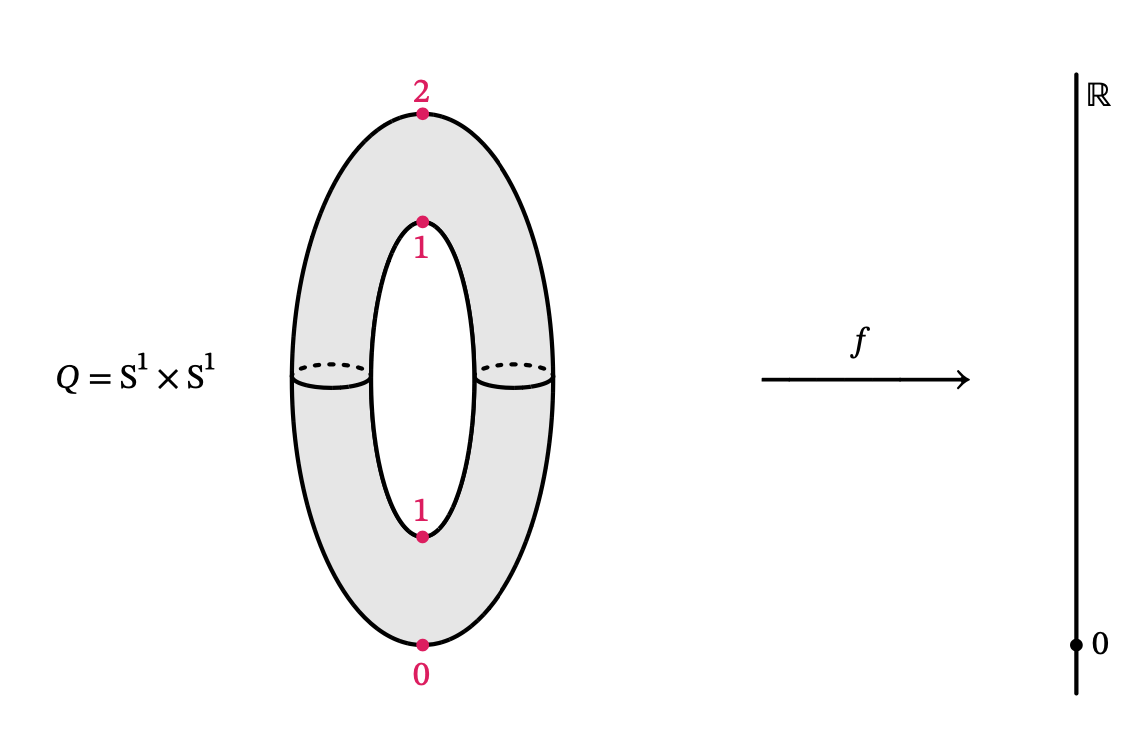
\includegraphics[width=9.3cm]{images/Lecture on Morse Theory/TORUS MORSE THEORY.png}
    \caption{Image of the Morse function of a torus from \cite{HiroLee2022}}
    \label{TORUS MORSE}
\end{figure}
Take as an example the projection map from the torus, see \ref{TORUS MORSE}. Here we have 4 special points: the top and bottom, and then the two points in the middle. What happens in these points is that the shape of the preimage changes:
\begin{itemize}
	\item the preimage of the top (and bottom) is a point
	\item the preimage of points between the top and middle point is a circle
	\item the preimage of the middle points is a wedge of circles
	\item the preimage of points between the middle points is a disjoint union of circles.
\end{itemize}
Note that at the special points the preimage is generally not a smooth manifold. These "special" points are critical points of $f$:
%TODO add what the strategy is

\begin{defn}[Critical point and critical value]
	Let $M$ be a closed $n$ manifold. A critical point of $f: M \to \R$ is a point $p \in M$ such that $(df)_p: T_p M \to T_{f(p)} \R \cong \R$ is \textit{not} surjective. 
	A critical value is the image of a critical point.
\end{defn}

\noindent The main goal then is to recover (up to diffeomorphism) $M$ from knowing the critical points and the behaviour in a neighborhood thereof. 


\noindent Firstly we can define what we mean by a "nice" function:
\begin{defn}
	A Morse function is a smooth map $f: M \to \R$ such that all critical points are nondegenerate, that is 
	$\Hess(f)_p := \left( \frac{\de^2 f}{\de x_i \de x_j}(p)\right)_{i,j}$
	is non-singular.
\end{defn}
\begin{rem}
	This is independent of the choice of chart. 
\end{rem}

\begin{ex}
	Let's start with a nonexample: the parabolic cylinder.
	%DRAWING
	\noindent With coordinates $x_1, x_2$, the Morse function drawn can be written as $f(x_1, x_2) = -x_1^2$.
	\noindent Then at every critical point the Hessian is given by
	\begin{equation}
		\Hess(f)_p = \begin{pmatrix}
			-2 & 0 \\
			0 & 0 
		\end{pmatrix}	
	\end{equation}
	which is clearly singular.

	\noindent Another nonexample is given by the function $f(x) = x^3$. Consider the map that goes from the graph of $f$ to its $y$ coordinate. Again the Hessian is singular at the critical point.
\end{ex}

%other example $f(x_1, x_2) = -x_1^2 -x_2^2$
% hessian is -2 0, 0 -2, two negative eigenvalues -> index -2

\noindent We're then interested in the local picture at a critical point.

\begin{defn}[Index of a critical point]
	If $p \in M$ is a nondegenerate critical point of $f : M \to \R$, the index of $f$ at $p$ is 
	\begin{equation}
		\ind_f (p) = \text{index of }\Hess(f)_p = \# \text{ negative eigenvalues of} \Hess(f)_p .
	\end{equation}
\end{defn}

\begin{ex}\label{ex:quadric}
	Consider the following basic examples: %DRAWINGS
	\begin{itemize}
		\item $f(x_1, x_2) = -x_1^2-x_2^2$, this has critical point $p=(0,0)$ and there the Hessian is given by
		$\begin{pmatrix}
			-2 & 0 \\
			0 & -2 
		\end{pmatrix}$. We therefore see that $p$ is nondegenerate and that $\ind_f (p) = 2$.
		\item $f(x_1, x_2) = -x_1^2+x_2^2$, very similar, but $\ind_f (p) = 1$,
		\item $f(x_1, x_2) = +x_1^2-x_2^2$, again $\ind_f (p) = 1$,
		\item $f(x_1, x_2) = +x_1^2+x_2^2$, now $\ind_f (p) = 0$.
	\end{itemize}
\end{ex}

\noindent The examples above are very important, because locally Morse functions are always of one of those forms.
\begin{lem}[Morse Lemma I]
	Let $p \in M^n$ be a nondegenerate critical point of $f: M^n \to \R$ of index $k$. Then there is a chart $(U, \phi)$ around $p$ such that the map $\tilde f$ defined as
	\begin{equation}
		\begin{tikzcd}
			U \ar[r, "\phi"] \ar[d, "f"]& \R^n \ar[dl, "\tilde f"] \\
			\R
		\end{tikzcd}
	\end{equation}
	is given by:
	\begin{equation}
		\tilde f (x_1, \dots, x_n) = f(p) - \sum_{i=1}^k x_i^2 + \sum_{j=k+1}^n x_j^2
	\end{equation}
\end{lem}

\begin{proof}[Idea of proof]
	Given a nondenerate critical point of index $k$ we only know that $\Hess(f)_p$ has $k$ negative eigenvalues, is nonsingular and is diagonalizable. That allows me to change the basis so that the function takes that form, essentially doing a Taylor expansion. In particular then the chart can be chosen such that the function is \textit{exactly} that expression.
\end{proof}

% -------------------------------------------------------------
% --------------------- LECTURE 6 13/11 -----------------------
% -------------------------------------------------------------

\noindent Given a Morse function $f: M \to \R$, $p \in M$, then we have the following immediate consequences of the lemma:
\begin{itemize}
    \item if $p$ is critical (non degenerate because of the \textit{Morse} function), because of the lemma we have a chart as above. Then the level sets $f^{-1} (f(p))$ look like a neighborhood of 0 in a quadric (locally).
    \item if $p$ is not critical (it's regular), by the implicit function theorem there are coordinates such that $f(x_1, \dots, x_n) = x_1$. So the level sets $f^{-1} (f(p))$ look like hyperplanes in $\R^n$ (locally).
\end{itemize}
This explains what we noticed initially for the example of the torus, that the level set changes when passing a critical point. In particular it always changes in one of the ways shown in \ref{ex:quadric}. This observation will be more complete after Morse Lemma II and Theorem \ref{thm:handle_attachment_morse} below.

The following theorem justifies the use of Morse theory to study manifolds.
\begin{thm}
    For any manifold Morse functions exist.
    \label{thm:morse_exist}
\end{thm}
\noindent It's not trivial but it can be proven with tools from differential topology.

Example of something we can prove with Morse functions:
\begin{thm}
	The Euler characteristic can be calculated by knowning the critical points and the corresponding indices of a Morse function:
    \begin{equation}
        \chi(M) = \sum (-1)^k c_k
    \end{equation}
    where $c_k$ is the number of critical points of index $k$.
\end{thm}
\noindent This is quite clear for the sphere and the genus $g$ surfaces with the usual Morse functions, but it's interesting that for \textit{any} Morse function we have this result.

The following theorem also seems very plausible from the drawings:
\begin{lem}[Morse Lemma II]
    Let $f: M \to \R$, $a< b \in \R$ such that $f$ does not have a critical value in $[a,b]$. Then
    \begin{equation}
        M_a = f^{-1} ((-\infty, a]) \hookrightarrow M_b = f^{-1} ((-\infty, b])
    \end{equation}
    is a deformation retract. In particular, it induces a diffeomorphism $f^{-1}(a) \cong f^{-1}(b)$.
\end{lem}
\noindent Concretely this tells us that the level set \textit{only} changes when crossing a critical point.
\begin{rem}
    The proof uses flow along vector field $\frac{\grad f}{|\grad f|}$... %DRAWING...
\end{rem}

We will restrict to the following class of Morse functions:
\begin{defn}[Admissibile Morse function]
    A Morse function $f: M \to [a,b]$ is admissibile if $\de M = f^{-1}(a) \cup f^{-1}(b)$ and $a,b$ are regular values.
\end{defn}
% but can I have im f = [a,c] with c<b and f^-1 (c) = emptyset?
\noindent The fact that they're regular values is important, since it gives us that a neighborhood of $f^{-1}(a)$ is diffeomorphic to a cylinder $f^{-1}(a) \times [0, \epsilon]$, i.e. a collar (and the same is true for a neighborhood of $f^{-1}(b)$). So an admissible Morse function naturally equips $M$ with the structure of a cobordism from $f^{-1}(a)$ to $f^{-1}(b)$.

\noindent Another useful theorem, analogous to \ref{thm:morse_exist} is the following:
\begin{thm}
    Admissible Morse functions exist.
\end{thm}
%TODO add reference to Kosinski Differentiable manifolds.

%tells us how the level set changes before and after the critical point
We would now like to know \textit{how} the level set changes before and after the critical point. In order to do this we first introduce the concept of handle attachment.
\begin{defn}[Handle attachment]
	Let $M^n$ be an $n$ manifold and let $H^j \coloneq D^j \times D^{n-j}$ for $j=0,1,\dots, n$. In addition let $f: \de D^j \times D^{n-j} \hookrightarrow \de M^n$ be an embedding and note that $\de D^j \times D^{n-j}$ also embeds into $H^j$. We can then \textit{attach a j-handle} to $M^n$ by gluing along $f$ to obtain the manifold 
	$M^n \amalg_f H^j$.
\end{defn}
\noindent This concept will be studied in one of the exercises. The following claim makes the definition meaningful:
\begin{clm}
    $M^n \amalg_f H^j$ has a smooth structure.
\end{clm}
\noindent Since we're interested in 2 manifolds, let's make explicit what it means to attach a $j$ handle to a 2 manifold:
\begin{itemize}%DRAWINGS
    \item $j=0, H^0 = D^0 \times D^2\cong D^2$ and we attach along the empty set (since $\de D^0 = \emptyset$), i.e. we take the disjoint union with $D^2$.
    \item $j=1, H^1 = D^1 \times D^1$ and we attach along $\de D^1 \times D^1$, i.e. along two segments
    \item $j=2, H^2 = D^2 \times D^0$ and we attach along $\de D^2 \times D^0\cong S^1$, i.e. along a circle
\end{itemize}
\noindent We can now see how the level sets change at a critical point.
\begin{thm}[\cite{Hirsch1976} Theorem 3.2, p.157]
\label{thm:handle_attachment_morse}
    Let $M^n$ be compact and $f: M^n \to [a,b]$ an admissible Morse function. Suppose that $f$ has a unique critical point $z$ of index $j$.

    \noindent There is an embedding $\iota: D^j \hookrightarrow M^n$ with image $e^j :=  \im \iota$ (called "belt disk"), satisfying: 
    \begin{itemize}
    	\item $z \in e^j$;
        \item $e^j \subset M^n \setminus f^{-1}(b)$;
        \item $f^{-1}(a) \cap e^j = \de e^j = \iota (\de D^j)$, this is also called "belt sphere";
        \item $M$ deformation retracts onto $f^{-1}(a) \cup e^j$.
    \end{itemize}
    The embedding can then be extended to $e^j \times D^{n-j}=: H^j$.
    %DRAWINGS
    We can now choose an $a'$ with $a<a'< f(z)$ and we then have
    \begin{equation}
        M^n \cong f^{-1}([a,a']) \cup_{\bbar \iota} H^j
    \end{equation}
    (for $n=2$ this is a unique diffeomorphism up to isotopy\footnote{See \ref{Isotopy} for the definition of isotopy.}).
\end{thm}
\noindent This theorem explains what happens to the level sets when we meet a critical point of index $j$: we attach a $j$ handle! 
To use the terms above: we extend the belt disk to a $j$ handle and attach it to the boundary by gluing along the belt sphere (which is also extended).
Of course, all the drawings presented are for 2 manifolds and we will only apply these results to such manifolds, but this theorem works more in general! 

\begin{ex}
\hfill%TODO not very clear
    \begin{itemize}
        \item index 0: $M=S^2$ % DRAWING
        we then have $e^0 = \{z\}$, $\iota: D^0={pt} \hookrightarrow M$ and $\bbar \iota: D^0 \times D^2 \hookrightarrow M$.
        \item Now what happens when attaching a 1-handle $\im \bbar \iota$? %DRAWING
        Chose: $D^{n-k} \hookrightarrow \de (S^1 \times [0,1] \amalg S^1 \times [0,1])$
        \item Start with $S^1 \times [0,1]$. Want to attach a 1-handle $D^1 \times D^1$. %DRAWING
        But now we can attach in two ways. With a simple band or with a twisted one.
        \item Let's start again with a cylinder and attach a 2-handle $D^2 \times D^0$, so I kind of close one of the two side of the cylinder. %DRAWING
        We see that the 1-handle and the 2-handle kind of cancel each other out!
        \item Analogously, starting with a disk and attaching a 0-handle and then a 1-handle, these also cancel each other out!
    \end{itemize}
\end{ex}

\begin{prop}[VI 7.1 in \cite{kosinski2013differential}, "Handle slides"]
    If $\tilde M := (M \coprod_f H^j) \coprod_g H^i$ and $i\leq j$, then $\tilde M$ can be obtained by first attaching $H^i$ and then $H^j$.
\end{prop}
\noindent Note that the word \textit{can} in the proposition is important: if we were to simply commute the two attachments $(M \coprod_g H^i) \coprod_f H^j$ we would get something that in general doesn't make sense, since the map $g$ goes into $M \coprod_f H^j$, not just $M$, and $H^i$ may no longer be attached at the boundary, leading to a space that is not even a manifold. The proposition instead says that there exist maps $\tilde g$ and $\tilde f$, into $M$ and $M \coprod_{\tilde g} H^i$ respectively, such that $(M \coprod_f H^j) \coprod_g H^i \cong (M \coprod_{\tilde g} H^i) \coprod_{\tilde f} H^j$.
\begin{ex} %DRAWING
\hfill
    \begin{itemize}
        \item $j=1, i=0$ 
        \item $j=2, i=1$ same picture but upside down!
        \item $j=i=1$ do it as an exercise.
    \end{itemize}
\end{ex}

\noindent What happens if $i>j$? In general it's not so simple, but if $i=j+1$ the following result holds.
\begin{prop}[VI 7.4 in \cite{kosinski2013differential}, "Handle cancellation"]
    Let $\tilde M := (M \coprod_f H^j) \coprod_g H^{j+1}$, where the attaching sphere of $H^{j+1}$ intersects the belt sphere of $H^j$ "transversely" in one point. Then $\tilde M \cong M$.
    %attaching sphere defined p 105 Kosinski but i don't understand how it's different from the belt sphere
\end{prop}
%Need M different from emptyset right??
\begin{ex}
    $j=0$ %DRAWING
\end{ex}


% -------------------------------------------------------------
% --------------------- LECTURE 7 15/11 -----------------------
% -------------------------------------------------------------

\begin{thm}[\cite{Hirsch1976} 8.3.4, p. 187]
    Let $M$ be a surface admitting a Morse function that has exactly two critical points. Then
    \begin{equation}
        M \cong S^2
    \end{equation}
\end{thm}
\begin{rem}
    In dimension 1,2 and 3 all the homeomorphic manifolds are also diffeomorphic. 
\end{rem}
\begin{proof}
    Because of the remark it's enough to prove the homeomorphism, rather than the diffeomorphism.

    \noindent Assume $p_+, p_- \in M$ are critical points. Since $M$ is compact, also $f(M)$ is compact and therefore has a maximum and a minimum, which exactly correspond to the two critical points. Now assume $p_+$ is the maximum, then $\ind p_+ = 2$. Now, because of Morse Lemma I we have $\exists U_+$ a neighborhood of $p_+$ with coordinates $x_1, x_2$ such that 
    \begin{equation}
        f|_{U_+} = -x_1^2 - x_2^2 + f(p_+)
    \end{equation}
    %DRAWING
    Then we have $\exists b < f(p_+)$ such that $D_+ = f^{-1}([b, +\infty)) \cong D^2$.

    \noindent Similarly, $\exists U_-$ a neighborhood of $p_-$ with coordinates $x_1, x_2$ such that 
    \begin{equation}
        f|_{U_-} = x_1^2 + x_2^2 + f(p_-)
    \end{equation}
    and now we have $\exists a > f(p_-)$ such that $D_- = f^{-1}((-\infty,a]) \cong D^2$.

    \noindent Let $B_+, B_-$ be disjoint caps around the poles of $S^2$ and denote $C := S^2 \operatorname{int} (B_+ \amalg B_-) \cong S^1 \times [0,1]$. % there was f,x star but I didn't understand TODO
    Now, notice $\de D_+ \cong S^1 \cong \de D_-$ and we have a diffeomorphism $h_0: D_+ \to B_+$ as they are both diffeomorphic to $D^2$. In addition $h_0 |_{\de D_+} \de D_+ \to \de B_+$.
    Notice that between $[a,b]$ there are no critical values, that is $f^{-1}([a,b])$ has no crtiical points
    Now, using Morse Lemma II we get:
    \begin{itemize}
        \item $f^{-1}((-\infty, b]) =: M_b \hookrightarrow M_a :=f^{-1}((-\infty, a])$, $f^{-1}(a) \cong f^{-1}(b)$
        \item $f^{-1}([a,b]) \cong f^{-1}(a) \times [0,1] \cong S^1 \times [0,1] $% again f,x star TODO
    \end{itemize}
    Now we can extend $h_0|_{\de D_+}$ to $h_1: \de D_+ \times [0,1] \to \de B_+ \times [0,1]$. Now we can glue $h_0$ and $h_1$
    \begin{equation}
        h: D_+ \cup (\de D_+ \times [0,1]) \to B_+ \cup (\de B_+ \times [0,1]) % TODO add what the two are isomorphic to
    \end{equation}
    \begin{clm}
        If $g: S^1 \to S^1$ is a homeomorphism, then it can be extended to a homeomorphism $\tilde g: D^2 \to D^2$.
    \end{clm}
    \noindent $\tilde g$ can simply be defined as follows
    \begin{equation}
        \tilde g(x) = 
        \begin{cases}
        	||x|| g\left(\frac{x}{||x||}\right), & \text{for } x\neq 0\\
        	0, & \text{for } x=0
        \end{cases}
    \end{equation}
    From the claim $h$ can be extended to a homeomorphism $M \to S^2$.
\end{proof}

\begin{rem}
\hfill
    \begin{enumerate}
        \item For any closed $n$ manifold that has two critical points, we have $M \cong S^n$ (\textit{homeomorphic}, not \textit{diffeomorphic}).
        \item (From Milnor) There are manifolds $M$ homeomorphic to a sphere but not diffeomorphic (e.g. $S^7$), we then talk about \textit{exotic spheres}.
    \end{enumerate}
\end{rem}

\begin{thm}[Classification of surfaces]\label{Classification of 2d manifolds}
    Let $M^2$ be an oriented, connected, closed surface. Then it can be obtained as in the following drawing:
    %DRAWING
\end{thm}

% -------------------------------------------------------------
% --------------------- LECTURE 8 20/11 -----------------------
% -------------------------------------------------------------

\begin{proof}
$ $ \newline  % to go to a new line after the word proof
    \indent Step 1: Choose an admissible Morse function $f$.
    
    Step 2a: If necessary, "perturb" $f$ to get distinct critical values. %DRAWING

    Step 2b: Chop into pieces with exactly one critical point and apply Morse Lemma I. We then get that $f^{-1}((-\infty, a_i])$ is obtained from $f^{-1}((-\infty,a_{i-1}])$ by attaching a handle.

    Goal: normal form (for closed connected surfaces) %DRAWING to explain from what to what we're going
    %why are copants still attaching a one handle??

    Step 3: Claim: We can obtain $M$ by first attaching 0-handles, then 1-handles, $\dots$, in ascending order.

    To prove this there are two strategies:
    \begin{enumerate}
        \item Use proposition about handle cancellation (first attaching $i$ handle and then $i+1$ handle these cancel) and handle slides: %DRAWING
        with these you can write down an algorithm to get the normal form from any handle decomposition.
        \item One can change the Morse function. Claim: We can choose $f$ such that if $\ind p_1 < \ind p_2 \implies f(p_1) < f(p_2)$. %DRAWING
        This can be proven by changing the Morse function locally around a critical point (see \cite{Hirsch1976} for more details). %TODO add ref
    \end{enumerate}

    Step 4: If $\de M = \emptyset$, then either $M = \emptyset$ or I have at least two critical points.

    \noindent Case 1: We have exactly 2 critical points which gives us $M \cong S^2$ because of Lemma. %TODO add ref

    \noindent Case 2: If we have $>2$ critical points, look at minimum, then there exist a neighborhood $D_-$ of the minimum such that $D_- \cong D^2$, i.e. a 0 handle attached to $\emptyset$ (because of Morse Lemma I $f$ locally looks like a cup).

    \noindent Starting from the minimum, attach one 0-handle. If then we attach another 0-handle, then we can use the handle slides and cancellations to get rid of all 0 handles but one.

    \noindent Next we can attach one handles and we have two options, %DRAWING
    only one of which gives an orientable manifold.

    \noindent At "end", same argument as for why only one 0-handle read backwards shows that we only have one 2-handle (for example change $f$ to $-f$).

    \noindent This ends the proof.
\end{proof}

Question: What about the unoriented case? (\textit{Hint: enough to have one attachment of Möbius strip})

We now consider the case with boundary:
\begin{thm}[Classification of surfaces with boundary]
    Let $M^2$ be an oriented, connected surface. Then it can be obtained as in the following drawing:
    %DRAWING
\end{thm}
\begin{proof}
	Now $ \de M \neq \emptyset$, then $\de M = S^1 \amalg \dots \amalg S^1$. If $f$ is an admissible Morse function $f$ onto $[a,b]$ with $f^{-1}(a) \cong (S^1)^{\amalg m}$ and $f^{-1}(b) \cong (S^1)^{\amalg n}$. Now one can prove that we need neither 0-handles (if $m \neq 0$) nor 2-handles (if $n \neq 0$).
\end{proof}


%Can this go with the cobordism part? /William
\section{More on cobordism groups}
\label{sec:more_on_cobordism_groups}

We now go back to cobordism groups to give some important results.

We had found 
\begin{align}
    &\Omega_0 \cong \Z_2 \\
    &\Omega_1 \cong 0    \\
    &\Omega_2 \cong \Z_2
\end{align}
while for the oriented case we have
\begin{align}
    &\Omega_0^{or} \cong \Z \\
    &\Omega_1^{or} \cong 0  \\
    &\Omega_2^{or} \cong 0
\end{align}
\begin{defn}[Commutative \Z-Graded Ring\footnote{Note that there is a difference between commutative graded ring and graded commutative ring! A commutative graded ring is a commutative ring that is graded (our notion), a graded commutative ring is a different notion that depends on the degree of homogeneous elements.}]
A commutative \Z-graded ring is a ring $R$ if there is a family of subgroups $\{R_n\}n\in\Z$ such that 
\begin{itemize}
\item the underlying abelian group can be decomposed as $R=\bigoplus_{n \in \Z} R_n$
\item $R_n \cdot R_k \subset R_{n+k}$ for all $n,k\in\Z)$
\end{itemize}
A non-zero element $x\in R_n$ is called a homogeneous element of $R$ of degree $n$.
\end{defn}

\begin{prop}
    $(\Omega_\bullet = \bigoplus_{n\geq 0} \Omega_n, \amalg, \times)$ is a commutative \Z-graded ring.
\end{prop}
\begin{proof}
    Firstly we need to check that the product respects the degree: this is true because $M^m \times N^n = (M \times N)^{m+n}$, so $[M\times N] \in \Omega_{m+n}$.

    \noindent Then the products descends to equivalence classes: if $Y_0 \simeq Y_1$ are cobordant via cobordism $(X,p)$ ($p:\de X \to {0,1}$), $M$ any manifold, then $\de X \times M = \de X \times M \xrightarrow{p \circ pr_X} \{0,1\}$. Therefore $(X \times M, p \circ pr_X)$ is a cobordism from $Y_0 \times M$ to $Y_1 \times M$.
\end{proof}

\begin{thm}[Thom]
    There is an isomorphism of \Z-graded commutative rings
    \begin{equation}
        \Omega_\bullet \cong \Z_2[x_2, x_4, x_5, x_6, x_8, \dots], \text{ with } \deg x_k = k, k \neq 2^i-1
    \end{equation}
    and the generators of the even degrees are given by $x_{2k} = [\R\P^{2k}]$.
\end{thm}
\begin{rem}
    Note that $(\deg x_2)^2 = \deg 4$ so maybe we could imagine that $\R\P^2 \times \R\P^2 \sim \R\P^4$ however that's not true since $x_2^2 \neq x_4$.
\end{rem}

There are versions for any tangential structure, such as orientation or stable framing.

\begin{thm}
    There is an isomorphism of \Z graded commutative rings:
    
    %TODO flip arrow
    \begin{equation*}
        \Omega_\bullet^{or} \otimes \Q \cong \Q[y_4, y_8, y_{12}, \dots]
    \end{equation*}
     $$  y_{4k}\mapsto [\C\P^{2k}]$$
     We write it in this way because in this case there is nontrivial torsion. We could also write
       $$ \Omega_\bullet^{or} /\text{torsion} \cong \Z[z_4, z_8, z_{12}, \dots]$$
    where the generators are given by Milnor hypersurfaces.
\end{thm}
%Now we have Stiefel-Whitney and Pontryagin numbers, which are cobordism invariants and hence determine classes of cobordisms.  In 1959, C.T.C. Wall proved that two manifolds are cobordant if and only if their Pontrjagin numbers and Stiefel numbers are the same % It is not clear to me what they are and what we are referring to just copied from the script, maybe should add explication /Andrea 
%TODO maybe say more
\begin{ex}
In particular, the groups in various degrees are given by the following list:
$$ \Omega_{0}^{\orient}=\Z$$
$$ \Omega_{1}^{\orient}=0$$
$$ \Omega_{2}^{\orient}=0$$
$$ \Omega_{3}^{\orient}=0$$
$$ \Omega_{4}^{\orient}=\Z$$
$$ \Omega_{5}^{\orient}=\Z_2$$
$$ \Omega_{6}^{\orient}=0$$
$$ \Omega_{7}^{\orient}=0$$
$$ \Omega_{8}^{\orient}=\Z\oplus\Z$$
$$ \Omega_{n\geq 9}^{\orient}\neq 0$$
For the last result see \cite[p. 203]{MilnorS05}.
%TODO maybe torsion comments
\end{ex}
%would be cool to write something why these are the case, but mysterious to me for now TBD /ANdrea
\subsection{Cobordism groups and the sphere spectrum \extra}\label{homotopyCob}
Very interestingly, the (stable) framed version is isomorphic to the stable homotopy groups of the sphere and it is \textit{not} computed to all degrees. This is one way to phrase a theorem named after Thom. It is fascinating because the stable homotopy groups of the sphere are central objects in stable homotopy theory. They are equivalently the homotopy groups of the sphere spectrum.

Now characterize spectra the bare minimum in order to talk about the sphere spectrum. Later,
after some detours in the magical world of $\infty$-categories, we will 
give a deeper sketch of what they are \ref{WhatSpectra}.
\begin{defn}[Suspension]
	Let $X$ be a pointed topological space. The suspension $\Sigma X$ of $X$ is the smash product of $X$
	 with $S^1$, i.e.
	$$\Sigma X=X\land S^1=\frac{X\times S^1}{(\{\ast\}\times S^1)\amalg X\times \{1\}}$$
\end{defn}
\begin{ex}
$\Sigma(S^1)=S^2$ more generally $\Sigma(S^n)=S^{n+1}$
\end{ex}
\begin{defn}[Sequential spectrum\footnote{Sometimes it is called just spectrum. We call it
		\emph{pre}spectrum in order to distinguish it from other notions with more structure, such as the suspension spectrum}]
	A sequential spectrum is a sequence of pointed spaces $\{X_k\}_{k\in\Z}$ with maps preserving basepoints
	 $\Sigma X_n\xrightarrow{\sigma_n}X_{n+1}$ called structure maps.
\end{defn}
\begin{defn}[Suspension Spectrum]
	The suspension spectrum $\Sigma^\infty X$ has $\Sigma_n$ as the $n$-th space in the sequence and structure maps $\Sigma\Sigma_n\cong\Sigma_{n+1}$.
\end{defn}
\begin{ex}[Sphere Spectrum]
	The sphere spectrum $\mathds{S}$ is the suspension spectrum of the point, $S^0$. In fact, $\Sigma S^0=S^1$, $\Sigma^2 S^0=\Sigma\Sigma S^0=\Sigma S^1=S^2$ and in general $\Sigma^n S^0=S^n $
\end{ex}

\begin{notat}[Stable Homotopy Groups of the Sphere]
	The stable homotopy groups of the sphere are the homotopy groups of the sphere spectrum. Alternatively, one can define them as the homotopy groups of the sphere $\pi_{n+i}(S^n)$ such that $n>i+1$. This latter
	 characterization explains why they are called 'stable': due to Freudenthal's suspension theorem, such homotopy
	 groups are independent of $n$.
\end{notat}
\begin{rem}
Note that the stable homotopy groups of the sphere can be made into a commutative \Z-graded ring via direct sums. We denote it with $\pi_{\bullet}(\mathds{S})$
$$\pi_{\bullet}(\mathds{S})=\bigoplus_{n\geq 0}\pi_{n}(\mathds{S})$$
\end{rem}
\begin{thm}[Thom's theorem]
	One way of phrasing Thom's theorem is
	$$\Omega_{\bullet}^{\fr}\cong\pi_{\bullet}(\mathds{S})$$
	This is also called Pontrjagin-Thom isomorphism.
\end{thm}
\begin{ex}
 We list some examples of such commutative rings.
 $$    \Omega^{fr}_0 \cong\Z$$
  $$\Omega^{fr}_1 \cong\Z_2$$
  $$\Omega^{fr}_2 \cong \Z_2 $$
  $$\Omega^{fr}_3 \cong\Z_{24}$$
  $$\Omega^{fr}_4 \cong 0$$
  $$\Omega^{fr}_5 \cong 0$$
  $$\Omega^{fr}_6 \cong\Z_2$$
  $$\Omega^{fr}_7 \cong \Z_{240},$$
  $$\Omega^{fr}_11 \cong\Z_{504}$$
  $$\Omega^{fr}_15 \cong\Z_{480}\oplus\Z_2$$
\end{ex}
%Would be cool to add something about Thom spectrum and Galatius-Madsen-Tillmann-Weiß theorem

% -------------------------------------------------------------
% --------------------- LECTURE 9 22/11 -----------------------
% -------------------------------------------------------------
\part{Topological field theories}
\chapter{A summary of category theory}
\section{A modern perspective on cobordisms}

A bordism invariant was characterized as a homomorphism from the cobordism group to some other abelian group. 
To extract the cobordism group from bordism we took the following steps:
\begin{enumerate}
	\item observed that being cobordant is an equivalence relation,
	\item considered the equivalence classes of closed $n$ manifolds up to $n+1$ cobordisms, obtaining the \textit{sets} $\Omega_n$,
	\item took such equivalence classes together with disjoint unions, resulting in an abelian group\footnote{And eventually in a \Z graded commutative ring, but this will not be as important for us from now on.}.
\end{enumerate} 
This strategy was the key for classifying manifolds up to cobordism. 
However, the cobordism groups merely record that \emph{there is} a bordism between two manifolds (since two manifolds are equivalent just if there is a bordism, independently of what kind of bordism it is), 
thereby forgetting other properties of the bordism itself. 
We swich now perspective and analyze a more sophisticated structure remembering \underline{how} two manifolds are cobordant, 
e.g. indicating the manifold that bounds them and the direction of the bordism: the symmetric monoidal category $\Bord_{n,n-1}$ where objects are $(n-1)$ manifolds and morphisms are $n$-cobordisms. This is an instance of a process called categorification\footnote{Sometimes, e.g. in the nLab, also called vertical categorification.}: adding categorical structure to things, 
e.g.\footnote{Note that although this way of categorifying is the most prominent one, it is strictly speaking not the only way to categorify, one could also go from category theory to higher category theory.} 
passing from set-theoretic notions like set or function  categorical ones like category or functor. 
The invariants will become in turn functors from $\Bord_{n,n-1}$ to categories of algebraic nature like $\Vect_k$, the category of vector spaces on a field $k$. 
Such categorified cobordism invariants are exactly topological field theories (TFTs). 

The following table summarizes the comparison between additional structures in the two perspectives:

\begin{center}
    \begin{tabular}{||c|c||}
    \hline
        $\Omega_n$ & $\Bord_{n,n-1}$ \\ [0.5ex]
         \hline\hline
         set & category \\
         \hline
         monoid & monoidal category \\
         \hline
         commutative monoid & symmetric monoidal category \\
         \hline
         abelian group & Picard groupoid \\
         \hline
    \end{tabular}
\end{center}
Analogous to the comparison between the set-theoretic and category-theoretic perspective, we could also have a linear-algebraic perspective. Since an associative algebra on a vector space is the parallel construction to a monoid with set, and a commutative algebra corresponds to a commutative monoid. The following table adds this perspective.
\begin{center}
    \begin{tabular}{||c|c||}
    \hline
        $\Omega_n$ & $\Vect_k$ \\ [0.5ex]
         \hline\hline
         set & vector space\\
         \hline
         monoid & associative algebra \\
         \hline
         commutative monoid & commutative algebra \\
         \hline
    \end{tabular}
\end{center}
We make both these comparisons more rigorous by later (\ref{MonObj}) showing that
\begin{enumerate}
    \item a monoid is a monoid object in the category of sets.
    \item an associative algebra is a monoid object in the category of $k$-vector spaces $Vect_k$
    \item a (\emph{strict}) monoidal category is a monoid object in the category of small categories Cat
\end{enumerate} 
The same holds for the commutative case, commutative monoids, commutative algebras and (\emph{strict}\footnote{We will also sketch a way how to get general symmetric monoidal categories, i.e. not necessarily strict, in an analogous way. See \ref{EAlg}.}) 
symmetric monoidal categories are all examples of commutative monoid objects (see \ref{CommMonObj}).

\section{Category theory language} % (fold)
\label{sub:cathegory_theory_language}

\begin{defn}
\label{Cat}
    A locally small\footnote{A category is locally small if every hom $\Hom_{\mathscr{C}}(X,Y)$ is not bigger than a set. A locally small category is small if the collection of objects is also a set. A large category is a category which is not small. A category is essentially small if it is locally small and the collection of isomorphism classes (collections of isomorphic objects, i.e. objects with a morphism between them which has a left- and right-inverse) is a set. Questions of size of collections play an important role in category theory. For example, one cannot naively take the set of all sets as the collection of objects of the category of sets because of famous set-theoretic paradoxes like Cantor's, Burali-Forti's or Russell's. See \cite{shulman2008set} for an account on possible set-theoretic foundations for category theory.} category $\mathscr{C}$ consists of the following data:
    \begin{itemize}
        \item A class $\ob(\mathscr{C})$ whose elements are called the \underline{objects of $\mathscr{C}$},
        \item For any $X, Y \in \ob(\mathscr{C})$ a set $Hom_{\mathscr{C}}(X,Y)$ whose elements are called \underline{morphisms} \underline{from $X$ to $Y$},
        \item For any objects $X,Y,Z\in \ob(\mathscr{C})$ a map\footnote{Note that we can simply define composition as a map between sets because we are working with a locally small category.}
        
        \begin{gather*}
            \Hom_{\mathscr{C}}(Y,Z)\times \Hom_{\mathscr{C}}(X,Y)\xrightarrow{\circ} \Hom_{\mathscr{C}}(X,Z) \\
            (g,f)\mapsto g\circ f
        \end{gather*}
        which is called \underline{composition} of morpisms,
        \item For every object $X\in \ob(\mathscr{C})$ an element $id_{X}\in \Hom_{\mathscr{C}}(X,X)$ called the \underline{identity} of $X$.
    \end{itemize}
    Such data must fulfill the following axioms: \begin{itemize}
        \item $\forall f\in \Hom_{\mathscr{C}}(X,Y), f\circ id_{X}=f=id_{Y}\circ f$ \hfill (unitality)
        
        \item $\forall f\in \Hom_{\mathscr{C}}(X,Y), g\in \Hom_{\mathscr{C}}(Y,Z), h\in \Hom_{\mathscr{C}}(W,Z)$:
        \begin{equation}
        	(h\circ g)\circ f=h\circ (g\circ f) \tag{associativity}
        \end{equation}
        \end{itemize}
\end{defn}

\begin{ex}
A few examples of categories are the following:
\begin{center}
	\begin{tabular}{l|l|l}
	category & objects & morphisms \\ \hline \hline
	Set & class of all sets & functions between sets \\ \hline 
	Mon & class of all monoids & monoid homomorphisms \\ \hline
	Grp & class of all groups & group homomorphisms \\ \hline
	AbGrp & class of all abelian groups & group homomorphisms \\ \hline
	Ring & class of all rings & ring homomorphisms \\ \hline
	Vect${}_k$ & class of all $k$ vector spaces & linear maps \\ \hline
	Alg${}_k$ & class of all algebras over $k$ & algebra homomorphisms \\ \hline
	Top & class of all topological spaces & continuous functions \\ \hline
	FinSet & class of all finite sets & functions between sets \\ \hline
	SmoothMfld & set of all smooth manifolds & smooth functions \\ 
	\end{tabular}
\end{center}
    \begin{enumerate}
        \item Let $(P,\leq)$ be  a set with a transitive and reflexive relation $\leq$ (a preordered set).
        Define a category $\mathbf{P}$ with: 
        $$\ob(\mathbf{P})=P$$
        $$ \Hom_{\mathbf{P}}(X,Y)=\begin{cases}
            \{\ast\} & \text{if } x\leq y \\
            \emptyset & \text{else}
        \end{cases}$$
        \item Given categories $\mathscr{C},\mathscr{D}$ we can define a category $\mathscr{C}\times\mathscr{D}$ (the product category) by:
        $$\ob(\mathscr{C}\times\mathscr{D})=\ob(\mathscr{C})\times \ob(\mathscr{D})$$
        $$\Hom_{\mathscr{C}\times\mathscr{D}}((X,Y),(X',Y'))=\Hom_{\mathscr{C}}(X,X')\times \Hom_{\mathscr{D}}(Y,Y')$$ 
        
        \item\label{CatOP}
        Given a category $\mathscr{C}$, define a category $\mathscr{C}^{op}$ by:
        $$\ob(\mathscr{C}^{op})=\ob(\mathscr{C})$$ 
        $$\Hom_{\mathscr{C}^{op}}(X,Y)=\Hom_{\mathscr{C}}(Y,X)$$ $$g\circ_{\mathscr{C}^{op}}f=f\circ_{\mathscr{C}}g$$  
        this is called the opposite category of $\mathscr{C}$.
    \end{enumerate}
\end{ex}
\begin{defn}
    An isomorphism $f\in \Hom(X,Y)$ is a morphism such that $\exists g \in \Hom(Y,X)$ with $g\circ f=id_{X}, f\circ g=id_{Y}$.
\end{defn}
\begin{defn}
    A groupoid is a category where each morphism is an isomorphism.
\end{defn}
\begin{ex}\label{Delooping Monoid}
	Let $\mathscr{C}$ be a category with $\ob(\mathscr{C})=\{\ast\}$. 
   
 	\noindent  Then, $(\Hom_{\mathscr{C}}(\ast,\ast),\circ)$ is a monoid since composition is associative and unital with neutral element given by the identity morphism $id_\ast$.
  %TODO I think the notation is usually just BM, not bold--You are probably right but I prefer to put it bold because sometimes it can be confusing, e.g. a bicategory is often denoted by 'B' and then the delooping of a bicategory becomes a one-object tricategory BB. There was also a case I can't remember where one couldn't discern Bs in a topology class. It is true that we'll probably not encounter any such confusing cases but I still prefer it because it shows that it is something "special". having said this, not a big issue for me however, if we change it to just nonbold B /Andrea
	Conversely, every monoid $(M,\cdot)$ defines a category $\mathbf{B}M$ with 
	$$\ob(\mathbf{B}M)=\{\ast\},\Hom_{\mathbf{B}M}(\ast,\ast)=M,m\circ_{\mathbf{B}M} m'=m\cdot m',id_{\ast}=1_{M}$$ 
	$\mathbf{B}M$ is called the delooping of the monoid $(M,\cdot)$
    \footnote{We will see a generalization of such deloopings for certain categories, monoidal categories (see \ref{MonCat}) where any monoidal category $\cat$, will be a one-object \emph{bi}category $\mathbf{B}\cat$ called the delooping $\cat$ (see \ref{DeloopingMonCat}).}.
    The same holds for groups and one-object groupoids: every group $(G,\cdot)$ defines a one-object groupoid $\mathbf{B}G$ and vice versa

    More generally, monoids of the form $(\Hom_\cat(X,X),\circ)$ are called endomorphism monoids and an interesting example thereof is endomorphism monoids in the category $\Top\!\Vect_k$ of topological vector spaces and continuous linear operators. Such endomorphism monoids $(\Hom_{\Top\!\Vect_{k}}(X,X),\circ)$ and submonoids thereof are called operator algebras. They are important in functional analysis and in quantum theory.
\end{ex}

\begin{defn}
        Let $\mathscr{C}$ and $\mathscr{D}$ be categories. A functor $F:\mathscr{C}\rightarrow\mathscr{D}$ consists of the following data: \begin{itemize}
        \item an assignment 
        \begin{align}
        	F:\ob(\mathscr{C})&\rightarrow \ob(\mathscr{D})\\
        	X&\mapsto F(X)
        \end{align}
        \item for every two objects $X,Y\in \ob(\mathscr{C})$ a map 
        \begin{align}
        	\Hom_{\mathscr{C}}(X,Y)&\rightarrow \Hom_{\mathscr{D}}(F(X),F(Y))\\
        	f&\mapsto F(f)
        \end{align}
    \end{itemize} 
    such that 
    \begin{itemize}
        \item $F(id_{X})=id_{F(X)}$
        \item $F(g\circ f)=F(g)\circ F(f)$
    \end{itemize}
\end{defn}

\begin{ex}
\label{ex:functor}
Some examples of functors:
    \begin{enumerate}
        \item\label{ForgetfulFunctors} There are forgetful functors \begin{itemize}
            \item $\Ring\rightarrow \Grp\rightarrow\ \Set$
            
            \noindent $(R,+,\cdot)\mapsto(R,+)\mapsto R$
            \item $\Ring\rightarrow \Mon$ 
            
            \noindent $(R,+,\cdot)\mapsto(R,\cdot)$
            \item $\Vect_{k}\rightarrow \AbGrp\rightarrow \Set$

            \item $\Alg_k\to \Vect_k$ where the multiplicative structure on algebras is forgotten
        \end{itemize}
        \item\label{Representations of Groups} An action of a group $(G,\cdot)$ on a set $X$ is a functor $A: \mathbf{B}G\xrightarrow{\rho} \Set$ where $A(\ast)=X$ and every $g\in \Hom_{\mathbf{B}G}(\ast,\ast)$ is mapped to an automorphism\footnote{It is an automorphism and not a simple endomorphism because of a very important property of functors: they preserve isomorphisms: given a functor $F:\cat\to\dat$, if $f\in \Hom_\cat(X,Y)$ is an isomorphism, then $F(f)\in \Hom_\dat(F(X),F(Y))$ is an isomorphism as well because $F(f^{-1})\circ F(f)=F(f^{-1}\circ f)=F(id_X)=id_{F(X)}$ and simmetrically, $F(f)\circ F(f^{-1})=id_{F(Y)}$. For example, this can be used in the converse direction to show that two topological spaces are not homeomorphic by sending them (with a functor) to their non-isomorphic fundamental group(oid)s.} on $X$, $\Hom_{\mathbf{B}G}(\ast,\ast)\rightarrow \Hom_{\Set}(X,X)$. By the same reasoning, a linear representation of a group $(G,\cdot)$ is a functor $\mathbf{B}G\rightarrow \Vect_k$ .
        \item Given functors $F:\mathscr{C}\rightarrow\mathscr{D}$ and $G:\mathscr{D}\rightarrow\mathscr{E}$, their composite $G\circ F:\mathscr{C}\rightarrow\mathscr{E}$ is also a functor: $G\circ F(X)=G(F(X)), G\circ F(f)=G(F(f))$.
        \item $id_{\mathscr{C}}:\mathscr{C}\rightarrow\mathscr{C}$  with $id_{\mathscr{C}}(X)=X, id_{\mathscr{C}}(f)=f$ is also a functor.
    \end{enumerate}
\end{ex}
\begin{rem}\label{1CatOfAllCats}
      Since the composition of functors is associative\footnote{Try to convince yourself that it is so!} and unital there is a category of all (small\footnote{Let $\mathscr{C},\mathscr{D}$ be categories, the collection of all functors $F:\mathscr{C}\rightarrow\mathscr{D}$ is generally a class. Hence the category of all categories without any restriction would not be a locally small category and thereby not a category according to our definition \ref{Cat}.  However, if $\mathscr{C}$ is small, then the collection of all functors $F:\mathscr{C}\rightarrow\mathscr{D}$ is a set. Therefore, the category of all small categories is indeed a category according to our definition of category.}) categories $\Cat$ whose objects are (small) categories and whose morphisms are functors. For the same reason we also have a category Gpd of (small) groupoids.
\end{rem}
\begin{ex}\extra
Some more examples related to topological spaces.
    \begin{enumerate}
    \item \label{PathConnFunct} Let $X$ be a topological space. Observe the following equivalence relation: $x\sim x'$ if and only if there is a continuous map $f:[0,1]\to X$, also known as "path", such that $f(x)=0$ and $f(x')=1$. Denote with $\pi_0(X)$ the set of equivalence classes of path-connected points, also known as the set of path-connected components, in $X$. This gives a functor\footnote{There is also a functor $\pi:\Top\to \Set$ sending topological spaces to the sets of their connected components.} $\pi_0:\Top\to \Set$
    \item Let $X$ be a topological space. Its fundamental groupoid $\pi_{\leq 1}$ is the groupoid having:
    \begin{itemize}
        \item the points of $X$ as objects, $\ob(\pi_{\leq 1}(X))=X$;
        \item $\Hom_{\pi_{\leq 1}(X)}(x,y)$ is given by equivalence classes of continuous paths from $x$ to $y$ that are homotopic\footnote{We later define a homotopy, see Example \ref{Homotopy} below.} relative to their endpoints. We can spell out what this means in the following way
    
    	$$\Hom_{\pi_{\leq 1}(X)}(x,y)= \frac{\{\gamma\in \Hom_{\Top}([0,1],X)|\gamma(0)=x,\gamma(1)=y\}}{\text{homotopy relative to }\de[0,1]}$$

    	\item For $x,y,z\in X$, composition of $[\gamma]\in \Hom_{\pi_{\leq 1}(X)}(x,y)$ and $[\eta]\in \Hom_{\pi_{\leq 1}(X)}(y,z)$ is given by the concatenation of paths with appropriate reparametrization, 
    
    	$$[\eta]\circ[\gamma]=[\gamma\ast\eta]$$
    
    \end{itemize} 
    Units are constant paths, i.e. $c:[0,1]\to X$ such that $\forall t\in[0,1], c(t)=x$. Additionally, this is indeed a groupoid since inverses are given by the same paths run in the opposite direction. We have a functor 
    $$\pi_{\leq 1}:\Top\to \Gpd$$ 
    
    \item Let $X$ be a topological space and $x\in X$ an arbitrary basepoint. The assignement of a fundamental group of $X$ at $x$, $\pi_1(X,x)$\footnote{\textit{Reminder}: $\pi_1(X,x)=\pi_0(\Omega_x(X))$, where $\Omega_x(X)$ is the based loop space of $X$ at $x$} is a functor $\pi_1:\Top\to \Grp$
    \end{enumerate}
\end{ex}

\section{Natural transformations} % (fold)
\label{sub:natural_transformations}

%Topological field theory as a categorification of a symmetric monoid. Should we explain coincisely what categorifying is and tell a story about how TFTs are categorified? /Andrea
\begin{defn}
    Given two functors $F,G: \cat \to \mathscr{D}$ a natural transformation from $F$ to $G$, $\alpha : F \Rightarrow G$ is a collection of morphisms indexed by objects in $\cat$, $\alpha_x: F(X) \to G(X)$ such that $\forall f: X\to Y$ in $\cat$ the following diagram commutes
    \[ \begin{tikzcd}
		{F(X)} & {G(X)} \\
		{F(Y)} & {G(Y)}
		\arrow["{F(f)}"', from=1-1, to=2-1]
		\arrow["{\alpha_X}", from=1-1, to=1-2]
		\arrow["{\alpha_Y}", from=2-1, to=2-2]
		\arrow["{G(f)}", from=1-2, to=2-2]
	\end{tikzcd}\]
    If for every $ X\in \ob(\cat)$, $\alpha_X$ is an isomorphism, then $\alpha$ is a natural isomorphism.
\end{defn}
\begin{rem}\label{FunctorsPreserveCommut}
    Note that because of functoriality, if a diagram commutes in $\cat$, then its image under a functor $F:\cat\to\dat$ also commutes in $\dat$. Let for example $g\circ f=h\circ l$, then $F(g)\circ F(f)=F(g\circ f)=F(h\circ l)=F(h)\circ F(l)$
\end{rem}
\begin{notat}\label{FunCat}
    Let $\cat$ and $\dat$ be categories. We denote with $\Fun(\cat,\dat)$ the functor category where objects are functors $\cat\to\dat$ and morphisms are natural transformations between such functors. We encounter soon an example of functor category, the category of $G$-linear representations, see Example \ref{Cat of representations} below.
\end{notat}
\begin{rem}\label{FunctorGroupoids}
    Note that given a category $\cat$ and a \emph{groupoid} $\dat$, then $\Fun(\cat,\dat)$ is a groupoid since every component of any natural transformation is invertible because they are morphisms in $\dat$ and therefore any natural transformation is a natural isomorphism.
\end{rem}
\begin{ex}%TODO complete examples
\label{ex:natural_trafos}
\hfill
\begin{enumerate}
    \item
    \label{Cat of representations}
    As we have seen in Example \ref{Representations of Groups} in \ref{ex:functor}, a linear representation of a group $G$ is a functor $\mathbf{B}G\to \Vect_k$. A morphism between $G-$representations $V$ and $W$, $f:V\to W$ is a $k-$linear map which is equivariant, i.e. $\forall g\in G, \forall v\in V$ we have $f(gv)=gf(v)$. Since linear representations are functors, one might wonder if a morphism between functors $V,W:\mathbf{B}G\to \Vect_k$, i.e. a natural transformation, is an equivariant map. Let $f:V\Rightarrow W$ be a natural transformation. Then, for any $g\in \Hom_{\mathbf{B}G}(\ast,\ast)$ the following diagram commutes
    \[ \begin{tikzcd}
		V(*) \ar[r, "f(*)"] \ar[d, "V(g) = g\cdot"'] & W(*) \ar[d, "W(g) = g\cdot"]\\
		V(*) \ar[r, "f(*)"] & W(*) 
	\end{tikzcd}\]
    and hence the map is equivariant, it does not matter if we first act on the vector space and subsequently apply the map or viceversa. 
    
    Since one can compose unitally and associatively natural transformations\footnote{By composining their components.}, if we take the collection of all functors $\mathbf{B}G\to \Vect_k$ and the natural transformations between them we get the category of linear representations of the group $G$. Such categories where the objects are functors are called functor categories. 
    %TODO is this next example correct?
    \item The determinant can also be seen as a natural transformation. Let $\Mat$ be the functor $\Ring \to \Mon$ taking a commutative ring $R$ to the monoid $\Mat(R)$ of matrices with coefficients in the ring $R$. Another such functor is the forgetful functor which forgets addition in the ring and forgets that the product is commutative $U: \Ring \to \Mon$. The determinant is then the following map of monoids:
    \begin{equation}
    	\begin{tikzcd}[row sep=small]
	    	\Mat(R) \ar[r, "\det"] & R \\
	    	M \ar[r, mapsto] & \det M
	    \end{tikzcd}
    \end{equation}
    The product rule for the determinant makes the map into a monoid homomorphism.
    The naturality diagram for rings $R,S$ for a map $f:R\to S$ is then the following:
    \begin{equation}
	    \begin{tikzcd}
	    	\Mat(R) \ar[r, "\det"] \ar[d, "\Mat(f)"']& R \ar[d, "f"]\\
	    	\Mat(S) \ar[r, "\det"] & S 
	    \end{tikzcd}
    \end{equation}
    In words, this means that to calculate the determinant with coefficients in $S$ we can proceed in two equivalent ways:
    \begin{itemize}
    	\item change coefficients from $R$ to $S$ and then calculate the determinant,
    	\item calculate the determinant using the matrix with $R$ coefficients and then map into $S$.
    \end{itemize}
    Instead of taking \textit{all} matrices we could take the general linear group $GL(-): \Ring \to \Grp$. In that case det is a natural transformation between $GL(-)$ and the functor $(-)^\times: \Ring \to \Grp$ taking the units in the ring.
    \item
    \label{Homotopy}
        Let $X,Y\in \Top$ and $f,g\in \Hom_{\Top}(X,Y)$. A homotopy from $f$ to $g$ is a continuous map 
        $$h:[0,1]\times X\to Y$$ 
        such that for every $x\in X, h(0,x)=f(x)$ and $h(1,x)=g(x)$. Two maps are homotopic if there is a homotopy between them. 
    	Although the homotopy seems intuitively like a map between maps, like the natural transformation is, this seems still very far from a natural transformation. However, there is an equivalent formulation of natural transformation, given below, which shows that homotopies and natural transformations are related. We will later show a way to make this comparison more rigorous, see \ref{Homotopy2Top}. 
\end{enumerate}
\end{ex}

\begin{defn}\extra\textmd{(Homotopy Analogue of Natural Transformation).}
    Let $\Delta^{1}$ be the category with two objects $0,1$ and one nonidentity morphism $u:0\to1$. Given two functors $F,G:\cat\to\dat$ we can see a natural transformation $\tau:F\Rightarrow G$ as a functor $N:\cat\times\Delta^{1}\to\dat$ where $N|_{\cat\times\{0\}}=F$ and $N|_{\cat\times\{1\}}=G$ and thus for every $X\in\cat$, $N(X,0)=F(X)$ and $N(X,1)=G(X)$. 
\end{defn}
\noindent This is equivalent to the previous definition for the following reason: let $X\xrightarrow{f} Y$ be an arbitrary arrow in $\cat$ and consider this commutative\footnote{It commutes because of unitality in both categories: $f\circ id_X=id_Y\circ f$ and $u\circ id_0=id_1\circ u$.} diagram in $\cat\times\Delta^1$
% https://q.uiver.app/#q=WzAsNCxbMCwwLCIoWCwwKSJdLFswLDEsIihZLDApIl0sWzEsMSwiKFksMSkiXSxbMSwwLCIoWCwxKSJdLFswLDMsIihpZF9YLHUpIl0sWzAsMSwiKGYsaWRfMCkiLDJdLFszLDIsIihmLGlkXzEpIl0sWzEsMiwiKGlkX1ksdSkiLDJdXQ==
\[\begin{tikzcd}
	{(X,0)} & {(X,1)} \\
	{(Y,0)} & {(Y,1)}
	\arrow["{(id_X,u)}", from=1-1, to=1-2]
	\arrow["{(f,id_0)}"', from=1-1, to=2-1]
	\arrow["{(f,id_1)}", from=1-2, to=2-2]
	\arrow["{(id_Y,u)}"', from=2-1, to=2-2]
\end{tikzcd}\]
The image of the latter diagram under $N$ is the following commutative diagram in $\dat$
% https://q.uiver.app/#q=WzAsNSxbMCwwLCJGKFgpIl0sWzAsMSwiRihZKSJdLFsxLDEsIkcoWSkiXSxbMSwwLCJHKFgpIl0sWzIsNF0sWzAsMywiTihpZF9YLHUpIl0sWzAsMSwiRihmKSIsMl0sWzMsMiwiRyhmKSJdLFsxLDIsIk4oaWRfWSx1KSIsMl1d
\[\begin{tikzcd}
	{F(X)} & {G(X)} \\
	{F(Y)} & {G(Y)} 
	\arrow["{N(id_X,u)}", from=1-1, to=1-2]
	\arrow["{F(f)}"', from=1-1, to=2-1]
	\arrow["{G(f)}", from=1-2, to=2-2]
	\arrow["{N(id_Y,u)}"', from=2-1, to=2-2]
\end{tikzcd}\]
Hence the components of $\tau$ are just the image under $N$ of the pairs of maps $(id,u)$, i.e. $\forall X\in\cat, \tau_X=N(id_X,u)$


\section{Equivalence of categories \extra} % (fold)
\label{sub:equivalence_of_categories}

We did not cover this topic in the lecture, but the concept of equivalence of categories is important for results such as \ref{thm:classif_of_1dtft}.
\begin{defn}
    Let $F:\mathscr{C}\rightarrow\mathscr{D}$ be a functor. $F$ is named \begin{enumerate}
        \item faithful if $\forall X,Y\in\mathscr{C}$ the map $\Hom_{\mathscr{C}}(X,Y)\rightarrow \Hom_{\mathscr{D}}(F(X),F(Y))$ is injective,
        \item full if $\forall X,Y\in\mathscr{C}$ the map $\Hom_{\mathscr{C}}(X,Y)\rightarrow \Hom_{\mathscr{D}}(F(X),F(Y))$ is surjective,
        \item fully faithful, if $F$ is full and faithful,
        \item conservative, if for $f:X\rightarrow Y$ in $\mathscr{C}$ such that if $F(f)$ is an isomorphism, then $f$ is an isomorphism,
        \item an isomorphism if $\exists G:\mathscr{D}\rightarrow\mathscr{C}$ such that $G\circ F=id_{\mathscr{C}}$ and $F\circ G=id_{\mathscr{D}}$,
        \item an equivalence if $\exists G:\mathscr{D}\rightarrow\mathscr{C}$ and natural isomorphisms $G\circ F\overset{\epsilon}{\cong}id_{\mathscr{C}}$ and $F\circ G\overset{\eta}{\cong}id_{\mathscr{D}}$,
        \item essentially surjective if $\forall Z\in\mathscr{D}, \exists Z'\in\mathscr{D}, X\in\mathscr{C}$ and an isomorphsim $F(X)\overset{f}{\cong}Z'$.
    \end{enumerate}
\end{defn}
% realized only writing down the definition of adjunction that I swapped unit and counit in the case of equivalence, will fix it, sorry! :/ /Andrea 
%what? /William
\begin{defn}[Equivalence and isomorphism of Categories]
    Two categories $\cat$ and $\dat$ are equivalent (isomorphic) if and only if there is an equivalence (isomorphism) between them.
\end{defn}
From the definition above we can see that equivalence of categories is a \textit{weaker} notion than that of being isomorphic. However finding naturally isomorphic categories is very rare, so the notion of equivalence is often more useful. Here we also use the term \textit{weak} which in category theory often refers to the substitution of an equality by an appropriate natural isomorphism.
\begin{notat}
    We denote that two categories $\cat,\dat$ are equivalent by $\cat\simeq\dat$. Whereas, we write down $\cat\cong\dat$ if they are naturally isomorphic, i.e. there is a natural isomorphism between them. 
\end{notat}
\begin{thm}[Fundamental Theorem of Category Theory\footnote{We call it fundamental theorem of category theory following \cite{RezkQuasiCat} to emphasize how important it is. It is central to category theory because it is often very interesting to prove that two categories are equivalent and virtually always one uses the "fully faithful and essentially surjective criterion". This is however an unorthodox denomination because usually such theorem just lacks a name.}]
    Two categories $\cat$ and $\dat$ are equivalent if and only if it there is a fully faithful and essentially surjective functor $F:\cat\to\dat$.
\end{thm}
\begin{proof}
$\implies$
Suppose that there is an equivalence between $\cat\xrightarrow{F}\dat$. Since it is an equivalence, there must be a functor $\dat\xrightarrow{G}\cat$ such that their compositions are naturally isomorphic to the identities on $\cat$ and $\dat$ thanks respectively to natural isomorphisms $\epsilon$ and $\eta$. Thus, for any $Y\in\dat$ there is an object $G(Y)\in\cat$ and an isomorphism $\epsilon_Y:(F\circ G)(Y)\to Y$ making $F$ essentially surjective. To prove the faithfulness of $F$ suppose that there is a pair of parallel arrows $f,g:X\to X'$ in $\cat$ that are mapped by $F$ to the same arrow in $\dat$, i.e. $F(f)=F(g)$, and hence having the following commuting diagram in $\cat$ because of the naturality of $\epsilon$
% https://q.uiver.app/#q=WzAsNixbMSwwLCJGKEcoWCkpIl0sWzEsMSwiRihHKFgnKSkiXSxbMCwwLCJYIl0sWzAsMSwiWCciXSxbMiwwLCJYIl0sWzIsMSwiWCciXSxbMCwxLCJGKEcoZikpPUYoRyhnKSkiLDFdLFsyLDAsIlxcZXRhX1giXSxbMiwzLCJmIiwyXSxbMywxLCJcXGV0YV97WCd9IiwyXSxbNCwwLCJcXGV0YV9YIiwyXSxbNCw1LCJnIl0sWzUsMSwiXFxldGFfe1gnfSJdXQ==
\[\begin{tikzcd}
	X & {G(F(X))} & X \\
	{X'} & {G(F((X'))} & {X'}
	\arrow["{G(F(f))=G(F(g))}"{description}, from=1-2, to=2-2]
	\arrow["{\epsilon_X}", from=1-1, to=1-2]
	\arrow["f"', from=1-1, to=2-1]
	\arrow["{\epsilon_{X'}}"', from=2-1, to=2-2]
	\arrow["{\epsilon_X}"', from=1-3, to=1-2]
	\arrow["g", from=1-3, to=2-3]
	\arrow["{\epsilon_{X'}}", from=2-3, to=2-2]
\end{tikzcd}\]
Note that $G\circ F\overset{\epsilon}{\cong}id_{\mathscr{D}}$, and so $\epsilon_X=id_X$, $\epsilon_{X'}\cong id_{X'}$. We can conclude that  $f=g$: $id_{X'}\circ f=G(F(g))\circ id_X$ and $id_{X'}\circ g=G(F(g))\circ id_X$ because of the commutativity of the latter diagram, thanks to unitality $f=G(F(g))=g$. To prove that $F$ is full take an arbitrary $g:F(X)\to F(X')$ in $\dat$ and consider the following diagram:
%https://q.uiver.app/#q=WzAsNCxbMSwwLCJHKEYoWCkpIl0sWzAsMCwiWCJdLFswLDEsIlgnIl0sWzEsMSwiRyhGKFgnKSkiXSxbMiwzLCJcXGVwc2lsb25fe1gnfSIsMl0sWzAsMywiRyhnKSIsMCx7Im9mZnNldCI6LTR9XSxbMSwwLCJcXGVwc2lsb25fWCJdLFsyLDMsIlxcY29uZyJdLFsxLDAsIlxcY29uZyIsMl0sWzEsMiwiZ157XFxhc3R9IiwyLHsic3R5bGUiOnsiYm9keSI6eyJuYW1lIjoiZGFzaGVkIn19fV0sWzAsMywiRyhGKGd7XFxhc3R9KSkiLDIseyJvZmZzZXQiOjN9XV0=
\[\begin{tikzcd}
	X & {G(F(X))} \\
	{X'} & {G(F(X'))}
	\arrow["{\epsilon_{X'}}"', from=2-1, to=2-2]
	\arrow["{G(g)}", shift left=4, from=1-2, to=2-2]
	\arrow["{\epsilon_X}", from=1-1, to=1-2]
	\arrow["\cong", from=2-1, to=2-2]
	\arrow["\cong"', from=1-1, to=1-2]
	\arrow["{g^{\ast}}"', dashed, from=1-1, to=2-1]
	\arrow["{G(F(g{\ast}))}"', shift right=3, from=1-2, to=2-2]
\end{tikzcd}\]
Since we can compose $\epsilon^{-1}_{X'}\circ G(g)\circ \epsilon_X$ there is an arrow $X\to X'$ and it is unique since the diagram commutes by naturality of $\epsilon$, we denote it by $g^{\ast}$. Also because of the commutativity of the latter diagram it must be the case that $G(F(g^{\ast}))=G(g)$ since $G(F(g^{\ast}))=\epsilon^{-1}_{X'}\circ G(g)\circ \epsilon_X=G(g)$. In the first part of the proof we proved the faithfulness of $F$ but by a specular argument, we could have proven the faithfulness of $G$. So, $g=F(g^{\ast})$ and thus $F$ is full. 

\noindent $\impliedby$ For every $Y\in\dat$ there is an isomorphic $F(X)$ because $F$ is essentially surjective and for every $X\in\cat$ there is an isomorphic $G(Y)$ because $G$ is essentially surjective, thus for every $Y\in\dat$ we can \emph{choose} an object $G(Y)\in\cat$ and an isomorphism between them. We denote the isomorphism by $\epsilon_Y:Y\cong F(G(Y))$. In order for $\epsilon_Y$ to be a natural transformation there must be a unique arrow such that for any $f:Y\to Y'$ in  $\dat$ the following diagram commutes 
    % https://q.uiver.app/#q=WzAsNCxbMCwwLCJGKEcoWSkpIl0sWzEsMCwiRihHKFknKSkiXSxbMCwxLCJZIl0sWzEsMSwiWSciXSxbMCwxLCJGKEcoZikpIiwwLHsic3R5bGUiOnsiYm9keSI6eyJuYW1lIjoiZGFzaGVkIn19fV0sWzAsMiwiXFxlcHNpbG9uX1kiLDJdLFsyLDMsImYiLDJdLFsxLDMsIlxcZXBzaWxvbl97WSd9Il1d
\[\begin{tikzcd}
	{F(G(Y))} & {F(G(Y'))} \\
	Y & {Y'}
	\arrow["{F(G(f))}", dashed, from=1-1, to=1-2]
	\arrow["{\eta_Y}"', from=1-1, to=2-1]
	\arrow["f"', from=2-1, to=2-2]
	\arrow["{\eta_{Y'}}", from=1-2, to=2-2]
\end{tikzcd}\]
 Then, we get an arrow $\eta_{Y'}^{-1}\circ f\circ\eta_Y:F(G(Y))\to F(G(Y'))$ making the the diagram commute, such an arrow exists because $F$ is full and is unique because $F$ is faithful. We denote it with $F(G(f))$. Now we prove that $G$ is actually a functor. Both $F(G(id_Y))$ and $F(id_{G(Y)})$ make the following diagram commute 
% https://q.uiver.app/#q=WzAsNCxbMCwwLCJGKEcoWSkpIl0sWzEsMCwiRihHKFkpKSJdLFswLDEsIlkiXSxbMSwxLCJZIl0sWzAsMSwiRihpZF97RyhZKX0pIiwwLHsib2Zmc2V0IjotMn1dLFswLDIsIlxcZXRhX1kiLDJdLFsyLDMsImlkX1kiLDJdLFsxLDMsIlxcZXRhX3tZfSJdLFswLDEsIkYoRyhpZF9ZKSkiLDIseyJvZmZzZXQiOjJ9XV0=
\[\begin{tikzcd}
	{F(G(Y))} & {F(G(Y))} \\
	Y & Y
	\arrow["{F(id_{G(Y)})}", shift left=2, from=1-1, to=1-2]
	\arrow["{\eta_Y}"', from=1-1, to=2-1]
	\arrow["{id_Y}"', from=2-1, to=2-2]
	\arrow["{\eta_{Y}}", from=1-2, to=2-2]
	\arrow["{F(G(id_Y))}"', shift right=2, from=1-1, to=1-2]
\end{tikzcd}\]
Since the diagram commutes $F(G(id_Y))=\eta_{Y}^{-1}\circ id_Y\circ\eta_{Y}=F(id_{G(Y)}$. Moreover, given $f:Y\to Y'$ and $f':Y'\to Y'$ consider the following commutative diagram 
% https://q.uiver.app/#q=WzAsNCxbMCwwLCJGKEcoWSkpIl0sWzEsMCwiRihHKFkpKSJdLFswLDEsIlkiXSxbMSwxLCJZJyciXSxbMCwxLCJGKEcoZidcXGNpcmMgZikpIiwwLHsib2Zmc2V0IjotMn1dLFswLDIsIlxcZXRhX1kiLDJdLFsyLDMsImYnXFxjaXJjIGYiLDJdLFsxLDMsIlxcZXRhX3tZJyd9Il0sWzAsMSwiRihHKGYnKVxcY2lyYyBHKGYpKSIsMix7Im9mZnNldCI6Mn1dXQ==
\[\begin{tikzcd}
	{F(G(Y))} & {F(G(Y''))} \\
	Y & {Y''}
	\arrow["{F(G(f'\circ f))}", shift left=2, from=1-1, to=1-2]
	\arrow["{\eta_Y}"', from=1-1, to=2-1]
	\arrow["{f'\circ f}"', from=2-1, to=2-2]
	\arrow["{\eta_{Y''}}", from=1-2, to=2-2]
	\arrow["{F(G(f')\circ G(f))}"', shift right=2, from=1-1, to=1-2]
\end{tikzcd}\]
By essentially the same argument we just provided for the functoriality of $F$ on the identities we get $F(G(f')\circ G(f))=\eta_{Y''}^{-1}\circ (f'\circ f)\circ\eta_Y=F(G(f'\circ f))$.

Now we just need to prove that there is a natural isomorphism $\epsilon:id_\cat\cong G\circ F$. Since $F$ is full and faithful we can find the components of $\epsilon$ by looking at their image under $F$. We denote $\eta^{-1}_F(X)$ by $F(\epsilon_X)$ and take into consideration a morphism $f:X\to X'$ from $\cat$ and the following commuting outer rectangle
% https://q.uiver.app/#q=WzAsNixbMCwwLCJGKFgpIl0sWzEsMCwiRihHKEYoWCkpKSJdLFswLDEsIkYoWCcpIl0sWzEsMSwiRihHKEYoWCcpKSkiXSxbMiwwLCJGKFgpIl0sWzIsMSwiRihYJykiXSxbMCwxLCJGKFxcZXBzaWxvbl9YKSJdLFswLDIsIkYoZikiLDJdLFsyLDMsIkYoXFxlcHNpbG9uX1gnKSIsMl0sWzEsMywiRihHKEYoZikpKSJdLFsxLDQsIlxcZXRhX3tGKFgpfSJdLFs0LDUsIkYoZikiXSxbMyw1LCJcXGV0YV97RihYJyl9IiwyXSxbMyw1LCJcXGNvbmciXSxbMSw0LCJcXGNvbmciLDJdXQ==
\[\begin{tikzcd}
	{F(X)} & {F(G(F(X)))} & {F(X)} \\
	{F(X')} & {F(G(F(X')))} & {F(X')}
	\arrow["{F(\epsilon_X)}", from=1-1, to=1-2]
	\arrow["{F(f)}"', from=1-1, to=2-1]
	\arrow["{F(\epsilon_{X'})}"', from=2-1, to=2-2]
	\arrow["{F(G(F(f)))}", from=1-2, to=2-2]
	\arrow["{\eta_{F(X)}}", from=1-2, to=1-3]
	\arrow["{F(f)}", from=1-3, to=2-3]
	\arrow["{\eta_{F(X')}}"', from=2-2, to=2-3]
	\arrow["\cong", from=2-2, to=2-3]
	\arrow["\cong"', from=1-2, to=1-3]
\end{tikzcd}\]
The right hand square commutes because of the naturality of $\eta$. Since the right hand square commutes $F(G(F(f)))=\eta^{-1}_{F(X')}\circ F(f)\circ \eta_{F(X)}$. Since the outer square commmutes $F(\epsilon_{X'})\circ F(f)=\eta^{-1}_{F(X')}\circ F(f)\circ \eta_{F(X)}\circ F(\epsilon_X)$. Thus, the left hand square commutes because $F(\epsilon_{X'})\circ F(f)=F(G(F(f)))\circ F(\epsilon_X)$ and thereby $\epsilon$ is natural because $\epsilon_{X'}\circ f=G(F(f))\circ \epsilon_X$ thanks to the faithfulness of $F$.
\end{proof}

\section{Adjunction \extra} % (fold)
\label{sub:adjunction}

\begin{defn}[Adjunction]\label{AdjFun}
    Let $F:\cat\to\dat$ and $G:\dat\to\cat$ be functors. We say that $F$ and $G$ form an adjunction if there are natural transformations $$\eta:id_{\cat}\Rightarrow G\circ F$$
    $$\epsilon:G\circ F\Rightarrow id_\dat$$
    that make the following two diagrams commute, $\forall X\in\cat$ for the first one and $\forall Y\in\dat$ for the second one 
	% https://q.uiver.app/#q=WzAsNCxbMCwwLCJGKFgpXFxjb25nIEYoaWRfe1xcY2F0fShYKSkiXSxbMSwxLCJGKEcoRihYKSkpIl0sWzIsMCwiaWRfXFxkYXQoRihYKSlcXGNvbmcgRihYKSJdLFsxLDMsIlxcYnVsbGV0Il0sWzAsMSwiRihcXGV0YV9YKSIsMl0sWzEsMiwiXFxlcHNpbG9uX3tGKFgpfSIsMl0sWzAsMiwiaWRfe0YoWCl9Il1d
	\[\begin{tikzcd}
		{F(X)= F(id_{\cat}(X))} && {id_\dat(F(X))= F(X)} \\
		& {F(G(F(X)))} \\
		\arrow["{F(\eta_X)}"', from=1-1, to=2-2]
		\arrow["{\epsilon_{F(X)}}"', from=2-2, to=1-3]
		\arrow["{id_{F(X)}}", from=1-1, to=1-3]
	\end{tikzcd}\]
	% https://q.uiver.app/#q=WzAsMyxbMCwwLCJHKFkpXFxjb25nIGlkX1xcY2F0KEcoWSkpIl0sWzEsMSwiRyhGKEcoWSkpKSJdLFsyLDAsIkcoaWRfXFxkYXQoWSkpXFxjb25nIEcoWSkiXSxbMCwxLCJcXGV0YV97RyhZKX0iLDJdLFsxLDIsIkcoXFxlcHNpbG9uX3tZfSkiLDJdLFswLDIsImlkX3tHKFkpfSJdXQ==
	\[\begin{tikzcd}
		{G(Y)= id_\cat(G(Y))} && {G(id_\dat(Y))= G(Y)} \\
		& {G(F(G(Y)))}
		\arrow["{\eta_{G(Y)}}"', from=1-1, to=2-2]
		\arrow["{G(\epsilon_{Y})}"', from=2-2, to=1-3]
		\arrow["{id_{G(Y)}}", from=1-1, to=1-3]
	\end{tikzcd}\]
	Equivalently, we could have asked that the following two diagrams commute, the first in $\Fun(\cat,\dat)$ and the second in $\Fun(\dat,\cat)$.
	% https://q.uiver.app/#q=WzAsNCxbMCwwLCJGXFxzaW1lcSBGXFxjaXJjIGlkX3tcXGNhdH0iXSxbMSwxLCJGXFxjaXJjIEdcXGNpcmMgRiJdLFsyLDAsImlkX1xcZGF0XFxjaXJjIEZcXHNpbWVxIEYoWCkiXSxbMSwzLCJcXGJ1bGxldCJdLFswLDEsIkYoXFxldGEpIiwyLHsibGV2ZWwiOjJ9XSxbMSwyLCJcXGVwc2lsb25fe0Z9IiwyLHsibGV2ZWwiOjJ9XSxbMCwyLCJpZF9GIiwwLHsibGV2ZWwiOjJ9XV0=
	\[\begin{tikzcd}
		{F= F\circ id_{\cat}} && {id_\dat\circ F= F} \\
		& {F\circ G\circ F} \\
		\arrow["{F(\eta)}"', Rightarrow, from=1-1, to=2-2]
		\arrow["{\epsilon_{F}}"', Rightarrow, from=2-2, to=1-3]
		\arrow["{id_F}", Rightarrow, from=1-1, to=1-3]
	\end{tikzcd}\]
	% https://q.uiver.app/#q=WzAsNCxbMCwwLCJHXFxzaW1lcSBpZF9cXGNhdFxcY2lyYyBHIl0sWzEsMSwiR1xcY2lyYyBGXFxjaXJjIEciXSxbMiwwLCJHXFxjaXJjIGlkX1xcZGF0XFxzaW1lcSBHIl0sWzIsMywiXFxidWxsZXQiXSxbMCwxLCJcXGV0YV97R30iLDIseyJsZXZlbCI6Mn1dLFsxLDIsIkcoXFxlcHNpbG9uKSIsMix7ImxldmVsIjoyfV0sWzAsMiwiaWRfe0d9IiwwLHsibGV2ZWwiOjJ9XV0=
	\[\begin{tikzcd}
		{G= id_\cat\circ G} && {G\circ id_\dat= G} \\
		& {G\circ F\circ G} \\
		\arrow["{\eta_{G}}"', Rightarrow, from=1-1, to=2-2]
		\arrow["{G(\epsilon)}"', Rightarrow, from=2-2, to=1-3]
		\arrow["{id_{G}}", Rightarrow, from=1-1, to=1-3]
	\end{tikzcd}\]
	We say that $F$ is left adjoint to $G$ denoted by $F\dashv G$, and reciprocally $G$ is right adjoint to $F$ denoted by $G\vdash F$.
	
	See \ref{HigherAdjFun} for an equivalent formulation\footnote{Although in the $\infty$-categorical 
	context, it is easily tranlatable by forgetting about the $\infty$s and substituting 'set' for
	'$\infty$-groupoid'.}
\end{defn}

\begin{ex}
	A trivial example is given by any functor that is an isomorphism. In that case the natural transformations are actually identities. 

	\noindent An equivalence of categories instead is in general \textit{not} an adjunction, however it can always be made into one by appropriately changing the natural isomorphisms. 

	\noindent The more typical examples are instead related to forgetful functors.
	%TODO add examples
\end{ex}


\section{Higher categories \extra}
\label{sub:higher_categories}

\begin{rem}
    We previously remarked that there is a category of all categories with functors as morphisms (\ref{1CatOfAllCats}). That was however not the end of the story since we also defined a morphism between functors, the natural transformation. Cat is in fact not just a "normal" category, also called a 1-category, but a strict 2-category, a category that also has morphisms between morphisms between objects and morphisms between objects compose up to strict equality\footnote{We remark soon after (see \ref{STRICT}) in which sense Cat is a \emph{strict} 2-category. See also for comparison the definition of Bicategory, a weak 2-category, \ref{Bicategory}.}. Morphisms between objects are called 1-morphisms and are functors in the case of $\Cat$. Morphisms between morphisms between objects are called $2$-morphisms and are natural transformations in the case of Cat. 
\end{rem}
\begin{notat}
    An $(n,k)$-category is a category in which all $m$-morphisms with $n\geq m>k$ are invertible and all $j$-morphisms with $j\leq k$ are not necessarily invertible.
\end{notat}
\noindent Following this convention an ordinary category is a strict $(1,1)$-category, a strict 2-category is a strict (2,2)-category, a groupoid is a strict (1,0) groupoid, and more generally an $n$-groupoid is an $(n,0)$-category. In order to make this more rigorous we need to loosely characterize enriched categories.
\begin{defn}[Loose definition of enriched category]\label{loose enriched Cat}
    Given a category $\dat$ a category $\cat$ enriched over $\dat$ is a category such that for every $X,Y\in\cat$ $$\Hom_{\cat}(X,Y)\in\dat$$
\end{defn}
\begin{rem}
    Note that this is just a loose characterization of what an enriched category is! For instance, one might wonder, how could we define the composition map, since for ordinary categories we defined it as a map of sets out of apt \emph{products} of Hom-sets. There is a way to sensibly talk about products of objects in many several other categories. We spell out the rigorous definition later on, see \ref{FullEnrichedCat}. We gave this loose characterization just to be able to characterize higher strict categories.
\end{rem}
\begin{ex}
	\hfill
    \begin{itemize}
        \item A locally small category is a category enriched over Set
        \item Cat is enriched over Cat, since instead of Hom-sets one has functor categories, which are themselves categories and hence in Cat. More generally categories with Hom-categories/functor categories instead of Hom-sets are called strict 2-categories, or (2,2)-categories following the convention we just stated.
        \item\label{2,1Grpd} Grpd is enriched over groupoid, since (as we previously remarked, see \ref{FunctorGroupoids}) all natural transformations between functors with a groupoid in the codomain are natural isomorphisms and therefore all functor categories (i.e. the Hom-objects of Grpd) are groupoids and hence in Grpd. One calls categories enriched over Grpd strict (2,1)-categories by the notational convention we just spelled out.
    \end{itemize}
\end{ex}
    
Having loosely characterized enriched categores We can provide a definition of strict $n$-categories. Following the notational convention we previously spelled out in a previous example, they amount to $(n,n)$-categories.
\begin{defn}\label{strict nCat}
    We define strict n-categories inductively. A 0-category is a set. A strict $n$-category is a category $\cat$ enriched in a (small\footnote{Because of size issues, as we remarked before, we work with locally small categories and the size of the $\Hom$ of any two objects cannot be greater than a set.}) strict $(n-1)$-category. This means that for any two $X,Y\in\cat$, $\Hom_{\cat}(X,Y)$ is not a set as usual, but a small strict $(n-1)$-category.
\end{defn}
\begin{ex}
	\hfill
	\begin{itemize} 
	    \item In the case that $n=1$ we end up with our usual definition of a (locally small) category (see \ref{Cat}).
	    \item  $\Cat$ is a $2$-category, in fact for any two $\cat,\dat\in \Cat$, $\Hom_{\Cat}(\cat,\dat)$ is a $1-$category, more specifically a functor category, i.e. a category where objects are functors and morphisms are natural transformations. Specifically:
	    $$\Hom_{\Cat}(\cat,\dat)=Fun(\cat,\dat)$$
	\end{itemize}
\end{ex}

\begin{rem}\label{STRICT}
    We call such categories, \emph{strict} n-categories because $(n-1)$-morphisms are strictly associative and unital, associativity and unitality hold with strict identities, on the nose. For example in Cat it holds that $\forall F:\cat\to\dat, id_\dat\circ F=F=F\circ id_\cat$ and $\forall F:\cat\to\dat, G:\dat\to\eat, H:\eat\to\bat$
    $$H\circ(G\circ F)=(H\circ G)\circ F.$$
\end{rem}
\noindent We will later encounter a notion of weak 2-category (see \ref{Bicategory}).

\section{Monoidal Categories}\label{MonCat}
Recall that a monoid is a group where not necessarily every element is invertible: a set $M$ with a distinguished object $e\in M$ called unit, also known as neutral element, and a map of sets $m: M\times M \to M$ such that $m$ is:
\begin{itemize}
    \item associative $$
    \forall a,b,c\in M, \quad m(m(a,b),c)=m(a,m(b,c))
$$
usually written
$$
   \forall a,b,c\in M, \quad (a \cdot b) \cdot c = a\cdot (b \cdot c)
$$
\item and unital with respect to $e$:
$$
     m(e, -) =\id(-), \quad m(-, e) =\id(-)
$$
where $\forall x\in M, id(x)=x$. The latter equation is usually written $$
\forall x\in M, \quad e\cdot x=x=x\cdot e
$$
\end{itemize}
A monoidal category generalizes this structure with respect to objects \emph{and} morphisms of a category.
\begin{defn}
    Let $\cat$ be a category. A monoidal structure on $\cat$ is
    \begin{itemize}
            \item (O) an object $\mathbb{1}_\cat \in \cat$,
            \hfill the \textit{unit}
        \item (M) bifunctor $\otimes: \cat \times \cat \to \cat$, 
            \hfill the \textit{tensor product}
        
        \item (A) a natural isomorphism $\alpha:- \otimes (- \otimes -)\Rightarrow(- \otimes -) \otimes -$ that witnesses associativity:
        % % https://q.uiver.app/#q=WzAsMyxbMCwwLCJcXG1hdGhzY3J7Q31cXHRpbWVzXFxtYXRoc2Nye0N9XFx0aW1lc1xcbWF0aHNjcntDfSJdLFsxLDAsIlxcYWxwaGEiXSxbMiwwLCJcXG1hdGhzY3J7Q30iXSxbMCwyLCIoLVxcb3RpbWVzLSlcXG90aW1lcy0iLDIseyJjdXJ2ZSI6M31dLFswLDIsIi1cXG90aW1lcygtXFxvdGltZXMtKSIsMCx7ImN1cnZlIjotM31dLFs0LDMsIiIsMix7InNob3J0ZW4iOnsic291cmNlIjoyMCwidGFyZ2V0IjoyMH19XV0=
            \[\begin{tikzcd}
            	{\mathscr{C}\times\mathscr{C}\times\mathscr{C}} & \alpha & {\mathscr{C}}
            	\arrow[""{name=0, anchor=center, inner sep=0}, "{(-\otimes-)\otimes-}"', curve={height=18pt}, from=1-1, to=1-3]
            	\arrow[""{name=1, anchor=center, inner sep=0}, "{-\otimes(-\otimes-)}", curve={height=-18pt}, from=1-1, to=1-3]
            	\arrow[shorten <=5pt, shorten >=5pt, Rightarrow, from=1, to=0]
            \end{tikzcd}\]
            \hfill the \textit{associator}
        \item (U) natural isomorphisms $\lambda:\mathbb{1}_\cat \otimes(-)\Rightarrow\id_\cat=(-)$ and $\rho:- \otimes\mathbb{1}_\cat\Rightarrow\id\cat=(-)$ witnessing unitality: % https://q.uiver.app/#q=WzAsNCxbMCwwLCJcXG1hdGhzY3J7Q30iXSxbMSwwLCJcXG1hdGhzY3J7Q30iXSxbMiwwLCJcXG1hdGhzY3J7Q30iXSxbMywwLCJcXG1hdGhzY3J7Q30iXSxbMCwxLCJcXG1hdGhiYnsxfVxcb3RpbWVzIC0iLDAseyJjdXJ2ZSI6LTJ9XSxbMCwxLCJpZF9cXG1hdGhzY3J7Q309KC0pIiwyLHsiY3VydmUiOjJ9XSxbMiwzLCJpZF9cXG1hdGhzY3J7Q309KC0pIiwyLHsiY3VydmUiOjJ9XSxbMiwzLCItXFxvdGltZXMgXFxtYXRoYmJ7MX0iLDAseyJjdXJ2ZSI6LTJ9XSxbNCw1LCJcXGxhbWJkYSIsMix7InNob3J0ZW4iOnsic291cmNlIjoyMCwidGFyZ2V0IjoyMH19XSxbNyw2LCJcXHJobyIsMix7InNob3J0ZW4iOnsic291cmNlIjoyMCwidGFyZ2V0IjoyMH19XV0=
            \[\begin{tikzcd}
            	{\mathscr{C}} & {\mathscr{C}} & {\mathscr{C}} & {\mathscr{C}}
            	\arrow[""{name=0, anchor=center, inner sep=0}, "{\mathbb{1}\otimes -}", curve={height=-12pt}, from=1-1, to=1-2]
            	\arrow[""{name=1, anchor=center, inner sep=0}, "{id_\mathscr{C}=(-)}"', curve={height=12pt}, from=1-1, to=1-2]
            	\arrow[""{name=2, anchor=center, inner sep=0}, "{id_\mathscr{C}=(-)}"', curve={height=12pt}, from=1-3, to=1-4]
            	\arrow[""{name=3, anchor=center, inner sep=0}, "{-\otimes \mathbb{1}}", curve={height=-12pt}, from=1-3, to=1-4]
            	\arrow["\lambda"', shorten <=3pt, shorten >=3pt, Rightarrow, from=0, to=1]
            	\arrow["\rho"', shorten <=3pt, shorten >=3pt, Rightarrow, from=3, to=2]
            \end{tikzcd}\]
            \hfill respectively the \textit{left and right unitors}
    \end{itemize}
    such that
    \begin{itemize}
        \item $\forall X,Y$ the following diagram commutes
        \[\begin{tikzcd}
	{(X\otimes\mathbb{1})\otimes Y} & {} & {X\otimes(\mathbb{1}\otimes Y)} \\
	& {X\otimes Y}
	\arrow["{\alpha_{X,\mathbb{1},\otimes Y}}", from=1-1, to=1-3]
	\arrow["{\rho_X\otimes id_Y}"', from=1-1, to=2-2]
	\arrow["{id_X\otimes\lambda_Y}", from=1-3, to=2-2]
\end{tikzcd}\]
        This diagram is called the triangle identity. It explains how the associator and the two unitors interact.
        \item $\forall W,X,Y,Z$ the following diagram commutes
       \[\begin{tikzcd}[cramped]
	&& {((W\otimes X)\otimes Y)\otimes Z} \\
	{} & {(W\otimes (X\otimes Y))\otimes Z} & {} & {(W\otimes X)\otimes (Y\otimes Z)} & {} \\
	& {W\otimes ((X\otimes Y)\otimes Z)} && {W\otimes (X\otimes (Y\otimes Z))}
	\arrow["{id_W\otimes \alpha_{X,Y,Z}}"', from=3-2, to=3-4]
	\arrow["{\alpha_{W,X,Y}\otimes id_Z}"', from=1-3, to=2-2]
	\arrow["{\alpha_{W,X\otimes Y,Z}}"', from=2-2, to=3-2]
	\arrow["{\alpha_{W\otimes X,Y,Z}}", from=1-3, to=2-4]
	\arrow["{\alpha_{W,X,Y\otimes Z}}", from=2-4, to=3-4]
\end{tikzcd}\]
        The latter diagram is called Mac Lane's pentagon. Thanks to \ref{thm:maclane_coherence} it pins down the associativity of more than 3 objects.
    \end{itemize}
\end{defn}
\begin{notat}
    As we usually abuse notation and denote monoids $(M,\cdot)$ just with $M$, although a monoid is a set \emph{equipped with} a binary operation; we will denote monoidal categories $(\cat,\otimes,\unit_\cat)$ just with $\cat$, although a monoidal category is a category \emph{equipped with} a monoidal structure.
\end{notat}
\begin{defn}[Strict Monoidal Category]
    A strict monoidal category is a monoidal category where objects and morphisms are associative and unital strictly, not up to specific natural isomorphisms, i.e. the associator and the left/right unitors are the identity. This means that for every $f:A,B,C\in\cat$ and every $f:A\to B, g:B\to C, h:C\to D\in\cat$ where $\cat$ is a strict monoidal category: \begin{itemize}
        \item $A\otimes(B\otimes C)=(A\otimes B)\otimes C$
        \item $A\otimes \mathbb{1}_\cat=A=\mathbb{1}_\cat\otimes A$
        \item $f\otimes(g\otimes h)=(f\otimes g)\otimes h$
        \item $f\otimes id_\mathbb{1_cat}=f=id_\mathbb{1_cat}\otimes f$
    \end{itemize}
\end{defn}
\begin{ex}[Examples of \emph{strict} monoidal categories]
\hfill
    \begin{itemize}
        \item Given an arbitrary category $\cat$, the set\footnote{A set and not a larger collection since we defined categories to be locally small.} of its endofunctors $\End(\cat,\cat)=\Hom_{\Cat}(\cat,\cat)$ are the objects of a monoidal category with morphisms given by natural transformations between them. The tensor product is given by composition and it is associative since composition of functors is associative. The monoidal unit is $id_\cat$ and is indeed left and right unital. Note however that this is an example of \emph{strict} monoidal category since functors compose strictly and not up to some associator and unitors.
        \item A monoid $(M,\cdot,e)$, seen as a category with objects $m \in M$ and only the identity morphisms, is a discrete strict monoidal category. The monoidal structure is simply given by multiplication of the elements of the monoid, which is clearly (strictly) associative and unital. A discrete category is a category where there are only identity morphisms. 
        %So, $(M,\cdot,e)=(\mathcal{M},\otimes,\mathbb{1}_\mathcal{M})$ where $\ob(\mathcal{M})=M$ and $\mathbb{1}_\mathcal{M}=e$.
    \end{itemize} 
\end{ex}
\begin{ex}[Examples of monoidal categories]
    Examples of monoidal categories are \begin{itemize}
        \item $(\AbGrp, \otimes)$
        \item $(\AbGrp, \oplus)$
        \item $(\Vect_k, \otimes)$
        \item $(\Vect_k, \oplus)$
        \item $(\Set, \coprod)$
        \item $(\Set, \times)$
        \item $(\Top, \times)$
        \item $(\Cat, \times)$
    \end{itemize}
\end{ex}

\subsection{Cartesian Categories: cartesian product \extra} 
\label{sub:cartesian_categories}

In particular,
 $(\AbGrp, \oplus), (\Vect_k, \oplus), (\Set, \times), (\Top, \times), (Cat, \times)$ are all examples of special monoidal categories: cartesian monoidal categories. A cartesian monoidal category is a monoidal category where the monoidal structure is given by a suitable notion of cartesian product in such category. We give a definition via a \textit{universal property} which is therefore valid for every category (although \textit{existance} must then be checked in the categories of interest).
\begin{defn}[Cartesian Product]\label{CartProd}
    Given $A,B\in\cat$, their cartesian product, if it exists, is the tuple $(A\times B,pr_1,pr_2)$, where $A\times B\in \ob(\cat)$ and $pr_1:A\times B\to A$  $pr_2:A\times B\to B$ such that for every other object $Y$ with morphisms $f:Y\to A$ and $g:Y\to B$ there is a unique morphism $u:Y\to A\times B$. This definition is summarised by the fact that the following commuting diagram 
    % https://q.uiver.app/#q=WzAsNSxbMSwwLCJZIl0sWzIsMSwiQiJdLFswLDBdLFswLDEsIkEiXSxbMSwxLCJBXFx0aW1lcyBCIl0sWzAsMSwiZyJdLFs0LDMsInByXzEiXSxbMCwzLCJmIiwyXSxbNCwxLCJwcl8yIiwyXSxbMCw0LCJcXGV4aXN0cyEgdSIsMSx7InN0eWxlIjp7ImJvZHkiOnsibmFtZSI6ImRhc2hlZCJ9fX1dXQ==
\[\begin{tikzcd}
	{} & Y \\
	A & {A\times B} & B
	\arrow["g", from=1-2, to=2-3]
	\arrow["{pr_1}", from=2-2, to=2-1]
	\arrow["f"', from=1-2, to=2-1]
	\arrow["{pr_2}"', from=2-2, to=2-3]
	\arrow["{\exists! u}"{description}, dashed, from=1-2, to=2-2]
\end{tikzcd}\]
\end{defn}
\noindent If we regard $\cat$ as a specific category such construction gives indeed rise to the expected notion of product in such a category: the cartesian product in $\AbGrp$ and $\Vect_k$ is indeed the direct sum, the cartesian product of sets with its projections in $\Set$, the product category in $\Cat$ and the product of spaces with the product topology in $\Top$. 

The following uniqueness property is typical of objects defined via a universal property:
\begin{lem}
\label{UptoIsoProds}
    Every product is unique up to isomorphism.
\end{lem}
\begin{proof}
    Suppose $(A\times B,pr_1,pr_2)$ and $(Y,f,g)$ are both products of $A,B\in\cat$. Then there are unique morphisms $u:A\times B\to Q$ and $u':Q\to A\times B$ such that the following diagram commutes
    % https://q.uiver.app/#q=WzAsNixbMSwwLCJZIl0sWzIsMSwiQiJdLFswLDBdLFswLDEsIkEiXSxbMSwxLCJBXFx0aW1lcyBCIl0sWzEsMiwiWSJdLFswLDEsImciXSxbNCwzLCJwcl8xIl0sWzAsMywiZiIsMl0sWzQsMSwicHJfMiIsMl0sWzAsNCwiXFxleGlzdHMhIHUiLDEseyJzdHlsZSI6eyJib2R5Ijp7Im5hbWUiOiJkYXNoZWQifX19XSxbNCw1LCJcXGV4aXN0cyF1JyIsMSx7InN0eWxlIjp7ImJvZHkiOnsibmFtZSI6ImRhc2hlZCJ9fX1dLFs1LDMsImYiXSxbNSwxLCJnIiwyXV0=
\[\begin{tikzcd}
	{} & Y \\
	A & {A\times B} & B \\
	& Y
	\arrow["g", from=1-2, to=2-3]
	\arrow["{pr_1}", from=2-2, to=2-1]
	\arrow["f"', from=1-2, to=2-1]
	\arrow["{pr_2}"', from=2-2, to=2-3]
	\arrow["{\exists! u}"{description}, dashed, from=1-2, to=2-2]
	\arrow["{\exists!u'}"{description}, dashed, from=2-2, to=3-2]
	\arrow["f", from=3-2, to=2-1]
	\arrow["g"', from=3-2, to=2-3]
\end{tikzcd}\]
Since everything commutes $f=f\circ u'\circ u$ and $g=g\circ u'\circ u$. Therefore, $u'\circ u=id_Y$ because $f=f\circ id_Y$ and $g=g\circ id_Y$ and $id_Y$ is the unique morphism such that the latter two equations hold.
\end{proof}
\begin{lem}
    The cartesian product is commutative up to isomorphism.
\end{lem}
\begin{proof}
    If $(A\times B,pr_1, pr_2)$ and $(B\times A,pr_1, pr_2)$ are both products of $A,B\in\cat$ then, they are isomorphic because of \ref{UptoIsoProds}.
\end{proof}
\begin{lem}
    The cartesian product is associative up to isomorphism.
\end{lem}
\begin{proof}
    Same reasoning as in the proof of the commutativity of the cartesian product.
\end{proof}
In a cartesian monoidal category $\cat$ the unit is a terminal object, i.e. an object $\ast\in\cat$ such that every object $X\in\cat$ has a unique morphism to it: $\exists !\phi_X:X\to\ast$. 
This is the case because given an arbitrary object $A\in\cat$ and a product with the terminal one $(A\times\ast,pr_1,pr_2)$ the units $\rho:A\times\ast\to A$ and $\lambda:\ast\times A\to A$ are the same projection $pr_1:A\times\ast\to A$ since the cartesian product is commutative. 
Such projection is indeed an isomorphism because $(A,id_A,\phi_A)$ is also a product of $\ast,A\in\cat$: any object $Y\in\cat$ with morphisms $f:Y\to A$ and $\phi_Y\to\ast$ has indeed a unique morphism into $A$ such that the diagram of the product commutes, namely $f$ itself. 
Thus, since both $(A\times\ast,pr_1,pr_2)$ and $(A,id_A,\phi_A)$ are products of the same two elements, they must be isomorphic because of \ref{UptoIsoProds}.

\noindent Hence, we see how any category with finite cartesian products is a monoidal category. Cartesian monoidal categories are in a sense special because they have some maps which are not possessed by every monoidal category, notably the diagonal map $\Delta_X:X\to X\times X$ and $\phi_X:X\to\mathbb{1}_\cat$ giving every object a comonoid structure. Moreover, they are all symmetric (defined later, \ref{SymmMonCat}) because the cartesian product is symmetric. 

\subsection{Noncartesian monoidal categories \extra} % (fold)
\label{sub:noncartesian_monoidal_categories}

%TODO I think if we want to say this it should be moved before /William
%Do you mean by 'this' the whole section? If so, I disagree since we need the cartesian product to define the tensor product in Ab and Vect via a universal property /Andrea
\begin{notat}
    We denote the category of abelian groups $\AbGrp$ also with Ab.
\end{notat}
\noindent In the previous paragraph, we have talked about cartesian monoidal categories and left out some examples of \emph{noncartesian} monoidal categories like $(\AbGrp,\otimes)$ and $(\Vect_k,\otimes)$. We now encounter some examples of noncartesian monoidal categories, which will be central in this class. They will be all similar to $(\AbGrp,\otimes)$, so we will first explain this category and then draw parallels with the others. To introduce the tensor product between abelian groups we first have to define what is a bilinear map:

\begin{defn}[Bilinear Map]
    For $A,B,C\in \Ab$, a bilinear map, aka group bihomomorphism, is a function $$f:A\times B\to C$$ which is a group homomorphism, aka linear map, in both arguments.
\end{defn}
\noindent An explanation of what happens to the elements of $A,B$ might be clearer. Note that a cartesian product $A\times B$ in Ab is an abelian group where the operation is 
$$(a_1,b_1)+(a_2,b_2)=(a_1+a_2,b_1+b_2).$$
So, we can spell out what it means to be a group bihomomorphism in the following way
\begin{defn}[Bilinear Map via Elements]
    A bilinear map is a function $f:A\times B\to C$ such that for all $a_1,a_2\in A$ and $b_1,b_2\in B$ it holds that 
    $$f(a_1+a_2,b_1)=f(a_1,b_1)+f(a_2,b_1)$$ and 
    $$f(a_1,b_1+b_2)=f(a_1,b_1)+f(a_1,b_2)$$
\end{defn}

Having defined what a bilinear map is, we can arrive at the definition of tensor product in Ab
\begin{defn}[Tensor Product of Abelian Groups]
    % The tensor product of abelian groups is an endofunctor $\otimes:\Ab\times\Ab\to\Ab$ which on objects $A$ and $B$ gives  $A\otimes B\in\Ab$ which has the following universal property: \begin{enumerate}
    %    \item there is a unique bilinear map $$\phi:A\times B\to A\otimes B$$ $$(a,b)\mapsto a\otimes b$$
    %    \item any other bilinear map out of $A\times B$, e.g. $h:A\times B\to C$, factors through $\phi$, i.e. there is a linear map $A\otimes B\xrightarrow{\bar{h}}C$ such that $h(a\times b)=\bar{h}(\phi(a,b))=\bar{h}(a\otimes b)$. This means that the following diagram commutes: 
    The tensor product of two abelian groups $A$ and $B$ is given by $(A \otimes B, \phi)$ where $A\otimes B$ is an abelian group and $\phi: A \times B \to A \otimes B$ is a bilinear map. $(A \otimes B, \phi)$ has the universal property that any bilinear map out of $A \times B$ factors uniquely through $A \otimes B$, i.e. $\forall C, h: A\times B \to C$ there is a unique linear map $\bbar h: A \otimes B \to C$ such that the following diagram commutes
       % https://q.uiver.app/#q=WzAsMyxbMCwwLCJWXFx0aW1lcyBXIl0sWzAsMSwiVlxcb3RpbWVzIFciXSxbMSwwLCJYIl0sWzAsMSwiXFxwaGkiLDJdLFsxLDIsIlxcYmFye2h9IiwyXSxbMCwyLCJoIl1d
\[\begin{tikzcd}
	{A\times B} & C \\
	{A\otimes B}
	\arrow["\phi"', from=1-1, to=2-1]
	\arrow["{!\bar{h}}"', from=2-1, to=1-2, dashed]
	\arrow["h", from=1-1, to=1-2]
\end{tikzcd}\]
\end{defn}

\noindent It can be equivalently defined via elements.
\begin{defn}[Tensor Product of Abelian Groups via Elements]
    For $A,B\in \Ab$ let $a,a'\in A$ and $b,b'\in B$ and consider the free abelian group on $A\times B$. Then, consider the free abelian group generated by elements of the form: 
    $$(a+a',b)-(a,b)-(a',b)$$
    $$(a,b+b')-(a,b)-(a,b').$$ 
    We denote such group by $R$. $A\otimes B$ is then the following  quotient: $A\otimes B=\frac{A\times B}{R}$.
\end{defn}

\section{Enriched categories \extra} % (fold)
\label{sub:Enriched categories}

Ab is very important as an enriching category. Before, we gave a loose characterization of what an enriched category is by just stating that the $\Hom$s are objects of whatever category we are enriching over. However, we glossed over an essential requirement: the category we are enriching on must be monoidal in order to define composition. We now give a fully satisfactory definition of an enriched category:
\begin{defn}[Enriched Category]\label{FullEnrichedCat}
    Given a \emph{monoidal} category $\dat$, a $\dat$-enriched category $\cat$, aka $\dat$-category or category enriched over $\dat$, is a category $\cat$ such that \begin{enumerate}
        \item $\forall X,Y\in\cat, \Hom_{\cat}(X,Y)\in\dat$. eW call $\Hom_\cat(X,Y)$ a Hom-object
        \item Composition is a morphism in $\dat$: $$\circ:\Hom_\cat(Y,Z)\otimes \Hom_\cat(X,Y)\to\Hom_\cat(X,Z)$$ 
        \item For any $X\in\cat$ there is 
        $$id_X:\unit_\dat\to \Hom_\cat(X,X)$$
        \item There is a Mac-Lane pentagon for Hom-objects in order to specify how $\circ$ is associative and two triangle diagrams in order to pin down how $\circ$ is left and right unital with respect to composable identity morphisms. One can check the spelled out diagram at definition 1.2.34 of \cite{land2021introduction} 
    \end{enumerate}
\end{defn}
\begin{ex}
	\hfill
	%TODO some examples already done before... /William True, did not notice, now I added that we are just recalling some, is it okay or better just \ref? /Andre
	We recall some examples spelled out before and provide a new one coming from topology (the last one):
    \begin{enumerate}\label{Examples of enriched categories (Simplicially)}
        \item A locally small category is a category enriched over Set. Set is a category enriched over itself.
        \item A $2$-category is a category enriched over Cat. Cat is a category enriched over itself, since Cat is a 2-category because $\Hom$s are functor \emph{categories}.
        \item A strict $n$-category is a category enriched over a strict $(n-1)$-category.
        \item A strict $(2,1)$-category is a category in which 2-morphisms are invertible and 1-morphisms not necessarily. It is a Grpd-enriched category. An example of (2,1)-category is Grpd itself, since all $\Hom_{\operatorname{Grpd}}$ are indeed  groupoids (see \ref{2,1Grpd} for an explanation). 
        \item A topologically enriched category is a category enriched over Top. The category of compactly generated Hausdorff spaces CGHaus, i.e. a category containing all $CW$-complexes, is a topologically enriched category, since one can take the mapping space $Map(X,Y)$ with the compact-open topology for any $X,Y\in \operatorname{CGHaus}$. Such categories can be used to model $(\infty,1)$-categories see \ref{HomotopyHypothesis} for a sketch of how this might work.
    \end{enumerate}
\end{ex}
There is an interesting example of strict (2,1)-category from topology and it will let us rigorously show in which sense a homotopy is a natural transformations and why one might want to talk
 about $\infty$-categories. Take a look at the following subsection for more on this \ref{ooHomotopyHypothesis}.

Having characterized satisfactorily enriched categories we can now define what is an Ab-enriched category.
\begin{defn}[Ab-Category]\label{Ab-Enriched Cat}
	An Ab-category, aka ringoid, Ab-enriched, $\cat$ is a category $\cat$ enriched over Ab. This is equivalent
	to saying that
	\begin{enumerate}
        \item $\forall X,Y\in\cat.\Hom_{\cat}(X,Y)\in\Ab$
        \item Composition is a morphism in $\Ab$: $$+:\Hom_\cat(Y,Z)\otimes_{\Ab} \Hom_\cat(X,Y)\to\Hom_\cat(X,Z)$$ such that it is associative and unital with respect to composable identity morphisms; in short $\Hom$-objects of $\cat$ posses an abelian structure with + as a binary operation
        \item The composition of the underlying $\Hom$-\underline{sets} is bilinear with respect to $+$, meaning that $\circ$ of $\Hom$-sets distributes over $+$ of $\Hom$-abelian groups i.e. $$f\circ(g+h)=(f\circ g)+(f\circ h)$$ $$(f+g)\circ h=(f\circ h)+(f\circ h)$$
    \end{enumerate}
\end{defn}
\begin{rem}
Note that in Ab-enriched categories there is an object $0$ such that it for any $X\in\cat$ there is a unique
 morphism $0\to X$ and a unique morphism $X\to 0$. This means that 0 is an initial and final object,
 such objects are usually called zero objects.
\end{rem}
\begin{ex}
\hfill
    \begin{itemize}
        \item A ring is a one object ringoid. More explicitly, a ring $(R,\cdot,+)=(\Hom_{\mathbf{B}R}(\ast,\ast),\circ,+)$  
        \item Ab is an Ab-category.
    \end{itemize}
\end{ex}

\begin{defn}[Additive category]
A category $\cat$ is additive if it is an Ab-enriched category such that it has finite coproducts.
\end{defn}
Note that in an Ab-enriched category, finite coproducts coincide with finite products, any finite product is a
finite coproduct and viceversa.
\begin{defn}[Abelian category]\label{AbelianCat}
A category $\cat$ is abelian if it is an additive category such that 
\begin{itemize}
	\item every morphism has kernel and cokernel
	\item every monomorphism is a kernel and every epimorphism is a cokernel, or equivalently,
	the evident map $\operatorname{Coim}(f)\to \operatorname{Im}(f)$ is an isomorphism
\end{itemize}
\end{defn}
\begin{rem}
    The category of abelian groups is very important for homological algebra, 
    a field with important applications to many fields, e.g. algebraic geometry (in particular intersection theory) and algebraic topology. The standard reference is \cite{weibel1994introduction}, check out part I of \cite{Mazel-Gee2024} for a modern introduction to the subject geared towards higher categorical generalizations. Such higher categorical generalizations are of major interest to us in the context of TFTs, we will later sketch for example how they can be used to calculate topological phases of matter (\ref{Spectra Phases of Matter}). 
\end{rem}
Another very important example for us of noncartesian\footnote{Interestingly, the fact that $\Vect_k$ is not cartesian and in particular $\operatorname{Hilb}_\mathbb{C}$ (the category of complex Hilbert spaces) is the main reason behind the no-cloning theorem from quantum information theory, more on this in \cite{baez2004quantum}. This characterizing non-cartesian aspect is nicely summarized by Freed in \cite{freed2012cobordism}, "We will see that a characteristic property of quantum systems is that disjoint unions map to tensor products. The passage from classical to quantum is (poetically) a passage from addition to multiplication, a kind of exponentiation."} monoidal category is $(\Vect_k,\otimes)$.
\begin{defn}[Tensor Product between Vector Spaces]
    The tensor product is usually defined from bases (see \hyperlink{https://en.wikipedia.org/wiki/Tensor_product}{wikipedia entry on tensor product}) or via quotient spaces\footnote{We use the definition via quotient spaces because it is easier to see that it fulfills the equivalent one via universal properties and the cartesian product.} along these lines: let $V,W\in \Vect_K$. Consider $L$, a vector space that has $V\times W$ as basis. Let $R$ be the subspace whose elements are linear combinations of one of the following forms
    $$(v+v',w)-(v,w)-(v',w)$$
    $$(v,w+w')-(v,w)-(v,w')$$
    $$(kv,w)-k(v,w)$$
    $$(v,kw)-k(v,w)$$
    where $v,v'\in V$, $w,w'\in W$ and $k\in K$. The tensor product is then the quotient space $L/R=V\otimes W$, where the image $(v,w)$ in this quotient is denoted by $v\otimes w$.

   \noindent The cartesian product construction helps us find an equivalent definition of the tensor product: it is an endofunctor $\otimes:\Vect_K\times\Vect_K\to\Vect_K$ where $V\otimes W$ has the following universal property: 
   \begin{enumerate}
       \item there is a unique bilinear map out of the cartesian product of the underlying sets $\phi:V\times W\to V\otimes W$
       \item any other bilinear map out of the cartesian product of the underlying sets $h:V\times W\to X$ factors through $\phi$:% https://q.uiver.app/#q=WzAsMyxbMCwwLCJWXFx0aW1lcyBXIl0sWzAsMSwiVlxcb3RpbWVzIFciXSxbMSwwLCJYIl0sWzAsMSwiXFxwaGkiLDJdLFsxLDIsIlxcYmFye2h9IiwyXSxbMCwyLCJoIl1d
		\[\begin{tikzcd}
			{V\times W} & X \\
			{V\otimes W}
			\arrow["\phi"', from=1-1, to=2-1]
			\arrow["{\bar{h}}"', from=2-1, to=1-2]
			\arrow["h", from=1-1, to=1-2]
		\end{tikzcd}\]
   \end{enumerate}
\end{defn}

As with Ab, $\Vect_k$ can also be used as enriching category.
\begin{defn}
     A linear category $\cat$, or algebroid, is a category enriched over $\Vect_k$.
\end{defn}
   
\begin{ex}
\hfill
    \begin{itemize}
        \item A $k$-algebra is a one object algebroid.
        \item $\Vect_k$ is a linear category, since also $\Hom_{\Vect_{k}}(X,Y)$ is a vector space
    \end{itemize}
\end{ex}

More generally the category of modules is also a very important example of noncartesian monoidal category.
\begin{defn}[Module]\label{CatOfModules}
    
\end{defn}
\begin{ex}
    The category of bimodules is an example of symmetric monoidal category
    \begin{defn}[Bimodule]\label{CatOfBimodules}
        
    \end{defn}
\end{ex}
Another example of non-cartesian monoidal category, which is not algebraic in nature but topological and will be useful for an outlook in the next section is the category of disks.
\begin{ex}\label{CatOfDisks}
    The category of oriented 1-dimensional open disks Disk$^{or}_{1}$ is also an important example of symmetric monoidal category for us in the context of TFTs. Recall that $D^1\cong (0,1)\cong\R$. 
    \begin{itemize}
        \item Its objects are finite disjoint unions of 1-dimensional open disks $$\emptyset,\qquad\R,\qquad\R\amalg\R,\qquad\dots,\qquad\R^{\amalg k}$$ with $k\in\N$ arbitrary.
        \item $\Hom_{\text{Disk}^{or}_{1,0}}(X,Y)$ consists of all smooth embeddings $j:X\hookrightarrow Y$ respecting orientations, i.e. there is an orientation preserving diffeomorphism from $X$ onto its image, .
        \item The tensor product is given by the disjoint union: given $X$ a disjoint union of $n$ oriented 1-disks and $Y$ a disjoint union of $m$ oriented 1-disks, $X\amalg Y$ is a disjoint union of $n+m$ oriented disks.
        \item The unit is the empty set since given an arbitrary disjoint union of disks $X$, $\emptyset\amalg X\cong X\cong X\amalg\emptyset$.
        \item There is a diffeomorphism $X\amalg Y\cong Y\amalg X$ making Disk$^{or}_{1,0}$ a \emph{symmetric} monoidal category.
    \end{itemize}  
    We will use it to give an equivalent definition of $k$-algebra (see \ref{EAlg}), but in general they can be used to define factorization algebras, a very important tool in the field of TFTs, see \cite{Tanaka_2020}.
\end{ex}
\subsection{Grothendieck's Homotopy Hypothesis and \texorpdfstring{$\infty$}{infinity}-categories \extra}\label{ooHomotopyHypothesis}
\begin{ex}\label{Homotopy2Top}
	We previously spelled out an analogue formulation of the natural transformation (see \ref{Homotopy}). This shows that the notion of homotopy and natural transformation are related. A way to more rigorously pin down that a homotopy is some kind of natural transformation is via the the homotopy 2-category of topological spaces. Instead of taking paths up to homotopies between paths, as in the more famous hTop, we take homotopies between paths up to homotopies between homotopies between paths. This results in a strict (2,1)-category h$_2$Top where objects are topological spaces, 1-morphisms are continuous maps and 2-morphisms are homotopies between continuous maps up to higher homotopies, i.e. homotopies between homotopies between continuous maps. A homotopy between a homotopy between continuous maps is defined in the following manner: given continuous functions $f,g:X\to Y$ and homotopies between them $k,h:X\times [0,1]\to Y$, a homotopy $L$ between these two homotopies $k$ and $h$ is a continuous function $L:X\times [0,1]\times[0,1]\to Y$ such that 
	\begin{itemize}
		\item $\forall t\in [0,1]\forall x\in X. H(0,t,x)=h(t,x)$
		\item $\forall t\in [0,1]\forall x\in X. H(1,t,x)=k(t,x)$
		\item $\forall t'\in [0,1]\forall x\in X. H(t',0,x)=f(x)$
		\item $\forall t'\in [0,1]\forall x\in X. H(t',1,x)=g(x)$
	\end{itemize}
	If one takes topological spaces as objects, continuous maps between them as 1-morphisms, and homotopies between continuous maps \emph{up to} homotopies between homotopies one gets the homotopy 2-category of topological spaces h$_2$Top and is an example of a strict $(2,1)$-category. If one restricts themselves to spaces admitting the structure of CW-complexes, i.e. something like weakly Hausdorff compactly generated spaces, and then take the homotopy 1-types thereof, we get a subcategory of  h$_2$Top called 2-1Type. Via the Eilenberg-MacLane space of a groupoid one can establish an equivalence of categories 
	$$2\operatorname{-}1Type\simeq Grpd$$
	This is Grothendieck's infamous homotopy hypothesis in dimension 1. It was formulated in \emph{Pursuing Stacks} in full generality for $\infty$-groupoids. We now sketch how this works in full glory.
\end{ex}
\begin{notat}
	By $\infty$-category we mean $(\infty,1)$-category.
\end{notat}
\begin{ex}\label{HomotopyHypothesis} Regarding the last example, one could ask why stop at homotopies between homotopies and not go all the way to homotopies between homotopies between homotopies, homotopies between ... for $\infty$ many times? This is a great question and also the way to provide a universal properties for constructions similar to the already seen cartesian product called homotopy co/limits (for more on this see chapters 1 and 2 of \cite{HarpazAlgebras}). In the end, one would get an $(\infty,1)$-category, a category in which the only morphisms that are not necessarily (weakly\footnote{To be precise, higher
		 morphisms in such a category are weakly invertible and not strictly. Weakly invertible means
		 that it is not the case the sense that $f\circ g=id$, but $f\circ g\simeq id$. This is not at all
		 negative. That things are not strict but up to homotopy/equivalence is exactly what one desires in this context.}) invertible are morphisms between objects, all other morphisms between morphisms are invertible; in other words, a category in which all $n>1$-morphisms are invertible and 1-morphisms not necessarily. 
	
	Moreover, one gets the fundamental $\infty$-groupoid of a space via a similar reasoning: instead of considering paths up to homotopies between paths, one can go all the way up and consider homotopies between homotopies between... without forgetting any information. All paths and all homotopies are clearly invertible so for all $k\in \mathbb{N}_0$ all $k$-morphisms are invertible and that is why it is called $\infty$-\emph{groupoid}. A synonym for $\infty$-groupoid is $(\infty,0)$-category. Note that the category of all $\infty$-groupoids is not an $\infty$-groupoids, because functors between $\infty$-groupoids are not necessarily invertible, parallelly to functors between 1-groupoids. The previously mentioned homotopy hypothesis states that the $(\infty,1)$-category of (nice) topological spaces we just sketched is equivalent to the $(\infty,1)$-category of $\infty$-groupoids. The intuition behinds this is that this should hold thanks to the construction of fundamental $\infty$-groupoids of spaces, whereas, in the other direction, from $\infty$-groupoids one can construct spaces via something called the geometric realization. This equivalence is the reason why in the literature the category of $\infty$-groupoids is sometimes called the category of Spaces. If the equivalence holds or not of course depends on how we define 'space' and $\infty$-groupoid, but it holds for many reasonable definitions, for instance a category of convenient topological spaces like the one of compactly generated weakly Hausdorff spaces. 
	
	Similarly to (2,1)-categories, which are enriched over ordinary groupoids, the sketchy idea
	behind an $(\infty,1)$-category is being enriched over $\infty$-groupoids.
	
	More concretely, one way to model this kind of categories with infinitely many invertible morphisms is with topologically enriched categories (which we previously described \ref{Examples of enriched categories (Simplicially)}), since mapping spaces are Hom-objects, 2-morphisms are paths 
	in such mapping spaces and higher morphisms are given by the homotopies between homotopies. 
	
	A further way is via some specific simplicially enriched categories, i.e. categories enriched with the cartesian monoidal category of simplicial sets sSet (sometimes denoted Set$_\Delta$). A synonym of simplicially enriched category is simplicial category. 
\end{ex}
\begin{defn}[The Simplex Category]
	We call simplex category, the category with all linearly ordered sets $[n]$ as objects and weakly monotonic maps as morphisms. We denote such category with $\Delta$.
\end{defn}
\begin{defn}[Simplicial Set]
	A simplicial set is a Set-valued presheaf on $\Delta$, i.e. a functor $X:\Delta^{\operatorname{op}}\to \Set$. Simplicial sets form a functor category where morphisms are natural transformations denoted sSet. It is bicomplete, see the proof in \cite[1.1.24]{land2021introduction}
\end{defn}
However, we do not want simplicial sets in general, but simplicial sets that are Kan complexes\footnote{See \url{https://ncatlab.org/nlab/show/Kan+complex}.}. This is because these special simplicial sets give a geometric model of $\infty$-groupoids and hence by enriching a category via such simplicial sets we get the desired $(\infty,1)$-category, similarly to getting (2,1)-categories by enriching with ordinary groupoids.

Quasi-categories are another construction to model $\infty$-categories that has been proven very useful and apt to create useful constructions. It also relies heavily on simplicial sets and there is strong connection to simplicially enriched categories (see \cite{land2021introduction}).

These three different ways to model $\infty$-categories are equivalent in some apt sense (see \cite{LurieGoodwillieEquivalent} and \cite{bergner2006survey}).

\begin{rem}
	Another important example of $(\infty,1)$-category is the category of spectra, a category similar\footnote{Abelian Groups:Algebra$\sim$Spectra:Higher Algebra, for more on this check out \cite{Mazel-Gee2024}.} to the category of abelian groups which we will encounter later (see \ref{Spectra Phases of Matter}).
\end{rem} 

\section{Objects Internal to a Monoidal Category}
\begin{defn}[Monoid Object]
    A monoid object in a monoidal category $\cat$ is an object $M\in\cat$ equipped with two distinguished morphisms, $\mu:M\otimes M\to M$ and $\eta:\mathbb{1}_\cat\to M$ called respectively multiplication and unit such that the following diagram commutes, so that the binary operation is associative 
    % https://q.uiver.app/#q=WzAsNSxbMCwwLCIoTVxcb3RpbWVzIE0pXFxvdGltZXMgTSJdLFsxLDAsIk1cXG90aW1lcyhNXFxvdGltZXMgTSkiXSxbMiwwLCJNXFxvdGltZXMgTSJdLFswLDEsIk1cXG90aW1lcyBNIl0sWzIsMSwiTSJdLFswLDEsIlxcYWxwaGFfe00sTSxNfSJdLFsxLDIsImlkX01cXG90aW1lc1xcbXUiXSxbMCwzLCJcXG11XFxvdGltZXMgaWRfTSIsMl0sWzMsNCwiXFxtdSIsMl0sWzIsNCwiXFxtdSJdXQ==
	\[\begin{tikzcd}
		{(M\otimes M)\otimes M} & {M\otimes(M\otimes M)} & {M\otimes M} \\
		{M\otimes M} && M
		\arrow["{\alpha_{M,M,M}}", from=1-1, to=1-2]
		\arrow["{id_M\otimes\mu}", from=1-2, to=1-3]
		\arrow["{\mu\otimes id_M}"', from=1-1, to=2-1]
		\arrow["\mu"', from=2-1, to=2-3]
		\arrow["\mu", from=1-3, to=2-3]
	\end{tikzcd}\]
    and the following also commutes, so that the binary operation is left and right unital
    % https://q.uiver.app/#q=WzAsNCxbMCwwLCJcXG1hdGhiYnsxfV9cXGNhdFxcb3RpbWVzIE0iXSxbMSwwLCJNXFxvdGltZXMgTSJdLFsyLDAsIk1cXG90aW1lc1xcbWF0aGJiezF9X1xcY2F0Il0sWzEsMSwiTSJdLFswLDEsIlxcZXRhXFxvdGltZXMgaWRfTSJdLFsyLDEsImlkX01cXG90aW1lc1xcZXRhIiwyXSxbMCwzLCJcXGxhbWJkYV9NIiwyXSxbMiwzLCJcXHJob19NIl0sWzEsMywiXFxtdSIsMV1d
	\[\begin{tikzcd}
		{\mathbb{1}_\cat\otimes M} & {M\otimes M} & {M\otimes\mathbb{1}_\cat} \\
		& M
		\arrow["{\eta\otimes id_M}", from=1-1, to=1-2]
		\arrow["{id_M\otimes\eta}"', from=1-3, to=1-2]
		\arrow["{\lambda_M}"', from=1-1, to=2-2]
		\arrow["{\rho_M}", from=1-3, to=2-2]
		\arrow["\mu"{description}, from=1-2, to=2-2]
	\end{tikzcd}\]
    Making multiplication associative and unital.
\end{defn}
\begin{ex}\label{MonObj}
	A monoid object is a 
    \begin{itemize}
        \item Monoid when in $(\Set,\times)$
        \item Algebra when in $(\Vect_k,\otimes)$
        \item Algebra when in $(BMod,\otimes)$
        %What is BMod /William
        \item \emph{Strict} monoidal category when in $(Cat,\times)$
        \item Topological monoids in $(\Top,\times)$
    \end{itemize}
\end{ex}
This example clarifies the parallel between monoids, algebras and monoidal categories we made at the start of this section. However, one could be bothered by the fact that we do not actually get a general monoidal category (i.e. not necessarily strict). To do this we will briefly talk about $\mathbb E_1$-algebras in section \ref{EAlg}.

\begin{defn}[Morphism of Monoids]
    Let $M,M'\in\cat$ be monoid objects $(M,\mu,\eta)$ and $(M',\mu',\eta')$. A morphism of monoids is a morphism $f:M\to M'$ such that both the following two diagrams commute 
    % https://q.uiver.app/#q=WzAsNyxbMCwwLCJNXFxvdGltZXMgTSJdLFswLDEsIk0iXSxbMSwxLCJNJyJdLFsxLDAsIk0nXFxvdGltZXMgTSciXSxbMiwwLCJcXG1hdGhiYnsxfV9cXGNhdCJdLFszLDEsIk0nIl0sWzMsMCwiTSJdLFswLDEsIlxcbXUiLDJdLFsxLDIsImYiLDJdLFswLDMsImZcXG90aW1lcyBmIl0sWzMsMiwiXFxtdSJdLFs0LDUsIlxcZXRhJyIsMl0sWzQsNiwiXFxldGEiXSxbNiw1LCJmIl1d
\[\begin{tikzcd}
	{M\otimes M} & {M'\otimes M'} & {\mathbb{1}_\cat} & M \\
	M & {M'} && {M'}
	\arrow["\mu"', from=1-1, to=2-1]
	\arrow["f"', from=2-1, to=2-2]
	\arrow["{f\otimes f}", from=1-1, to=1-2]
	\arrow["\mu'", from=1-2, to=2-2]
	\arrow["{\eta'}"', from=1-3, to=2-4]
	\arrow["\eta", from=1-3, to=1-4]
	\arrow["f", from=1-4, to=2-4]
\end{tikzcd}\]
\end{defn}
\begin{defn}[Comonoid Object]\label{ComonObj}
    Let $M\in\cat$, $M$ together with a comultiplication $\Delta$ and a counit $\epsilon$ is a comonoid object iff $(M,\mu,\eta)$ a monoid object in $\cat^{op}$ (see \ref{CatOP}) such that $\mu=\Delta^{op}$ and $\eta=\epsilon^{op}$. Straightforwardly, the definition we gave for monoid object, but with all the arrows inverted. 
\end{defn}

\begin{defn}[Bimonoid Object]\label{BimonObj}
    A bimonoid object in a monoidal category $\cat$ is simultaneously a monoid and a comonoid object in $\cat$ in a compatible way. It has a unit $\eta:\mathbb{1}_\cat\to M$ and a counit $\epsilon:\cat\to\mathbb{1}_\cat$, a multiplication $\mu:M\otimes M\to M$ and and a comultiplication $\Delta:M\to M\otimes M$ such that comultiplication and multiplication are morphisms of monoids. In the case of comultiplication, this means that given a monoid object $(M\otimes M,\mu',\eta')$ with $\mu':(M\otimes M)\otimes(M\otimes M)\to M\otimes M$ and $\eta':M\otimes M\to \mathbb{1}_\cat$  both the following diagrams commute 
    % https://q.uiver.app/#q=WzAsNyxbMCwwLCJNXFxvdGltZXMgTSJdLFswLDEsIk0iXSxbMSwxLCJNXFxvdGltZXMgTSJdLFsxLDAsIihNXFxvdGltZXMgTSlcXG90aW1lcyhNXFxvdGltZXMgTSkiXSxbMiwwLCJcXG1hdGhiYnsxfV9cXGNhdCJdLFszLDEsIk1cXG90aW1lcyBNIl0sWzMsMCwiTSJdLFswLDEsIlxcbXUiLDJdLFsxLDIsIlxcRGVsdGEiLDJdLFswLDMsIlxcRGVsdGFcXG90aW1lcyBcXERlbHRhIl0sWzMsMiwiXFxtdSciXSxbNCw1LCJcXGV0YSciLDJdLFs0LDYsIlxcZXRhIl0sWzYsNSwiXFxEZWx0YSJdXQ==
\[\begin{tikzcd}
	{M\otimes M} & {(M\otimes M)\otimes(M\otimes M)} & {\mathbb{1}_\cat} & M \\
	M & {M\otimes M} && {M\otimes M}
	\arrow["\mu"', from=1-1, to=2-1]
	\arrow["\Delta"', from=2-1, to=2-2]
	\arrow["{\Delta\otimes \Delta}", from=1-1, to=1-2]
	\arrow["{\mu'}", from=1-2, to=2-2]
	\arrow["{\eta'}"', from=1-3, to=2-4]
	\arrow["\eta", from=1-3, to=1-4]
	\arrow["\Delta", from=1-4, to=2-4]
\end{tikzcd}\]
We leave the case of the counit for the reader.
\end{defn}
%I don't think it's a bimonoid, i think it's just monoid and comonoid, without the additional property /William You are very right!!!!!!
\begin{defn}[Frobenius Algebra]\label{FrobAlg}
    A Frobenius algebra in an arbitrary monoidal category $\cat$ is simultaneously a monoid and a comonoid object in $\cat$ with a compatibility condition different from the one above: 
    $$(\mathbb{1}_\cat\otimes\mu)\circ(\Delta\otimes\mathbb{1}_\cat)=\Delta\circ\mu=(\mu\otimes\unit_\cat)\circ(\unit_\cat\otimes\Delta)$$
    called the Frobenius relation. 
\end{defn}

\begin{defn}[Group Object]\label{GroupObj}
    A group object in a cartesian monoidal category $\cat$ is a monoid object $M$ that also has an inverse map $(-)^{-1}:M\to M$ such that the following diagram commutes, meaning that the inverse behave as expected 
    % https://q.uiver.app/#q=WzAsNCxbMCwwLCJNIl0sWzEsMCwiTVxcdGltZXMgTSJdLFswLDEsIk1cXHRpbWVzIE0iXSxbMSwxLCJNIl0sWzAsMSwiKC0pXnstMX1cXHRpbWVzIGlkX00iXSxbMCwyLCJpZF9NXFx0aW1lcyAoLSleey0xfSIsMl0sWzIsMywiXFxtdSIsMl0sWzEsMywiXFxtdSJdLFswLDMsImlkX00iLDFdXQ==
\[\begin{tikzcd}
	M & {M\times M} \\
	{M\times M} & M
	\arrow["{(-)^{-1}\times id_M}", from=1-1, to=1-2]
	\arrow["{id_M\times (-)^{-1}}"', from=1-1, to=2-1]
	\arrow["\mu"', from=2-1, to=2-2]
	\arrow["\mu", from=1-2, to=2-2]
	\arrow["{id_M}"{description}, from=1-1, to=2-2]
\end{tikzcd}\]
\end{defn}
\begin{ex}\label{TopologicalGroup}
	\begin{itemize}
\item A topological group is a group object in Top
\item   A Lie group is a group object in $\SmoothMfld$
\item A group is a group object in Set
	\end{itemize}
\end{ex}

% -------------------------------------------------------------
% --------------------- LECTURE 10 27/11 -----------------------
% -------------------------------------------------------------
\section{Symmetric Monoidal Categories} % (fold)
\label{sub:symmetric_monoidal_categories}

In order to get the categorical parallel of a commutative monoid, we need to define a \emph{symmetric} monoidal category. We want to achieve something similar to $a \cdot b = b \cdot a$ in a monoid. However, we will not characterize this behavior with strict identities, but with a natural isomorphism\footnote{Just as we did for associativity and unitality.}. Given the functor 
$$swap:\cat\to\cat$$
$$swap:(X,Y)\mapsto (Y,X)$$
$$swap:(f,g)\mapsto (g,f)$$
we could try to achieve our objective with a natural isomorphism $\beta:\otimes\to\otimes\circ swap$ that can be visualized in the category of all categories Cat with the following diagram

% https://q.uiver.app/#q=WzAsMixbMCwwLCJcXGNhdFxcdGltZXNcXGNhdCJdLFsxLDAsIlxcY2F0Il0sWzAsMSwiXFxvdGltZXMiLDAseyJjdXJ2ZSI6LTN9XSxbMCwxLCJcXG90aW1lc1xcY2lyYyBzd2FwIiwyLHsiY3VydmUiOjN9XSxbMiwzLCJcXGJldGEiLDAseyJzaG9ydGVuIjp7InNvdXJjZSI6MjAsInRhcmdldCI6MjB9fV1d
\[\begin{tikzcd}
	\cat\times\cat & \cat
	\arrow[""{name=0, anchor=center, inner sep=0}, "\otimes", curve={height=-18pt}, from=1-1, to=1-2]
	\arrow[""{name=1, anchor=center, inner sep=0}, "{\otimes\circ\, swap}"', curve={height=18pt}, from=1-1, to=1-2]
	\arrow["\beta", shorten <=5pt, shorten >=5pt, Rightarrow, from=0, to=1]
\end{tikzcd}\]

However, this does not characterize an actually symmetric structure, but rather a \textit{braiding}, meaning that inverting two times the order of two tensor multiplied elements, i.e. objects or morphisms, does not necessarily equal the original tensor product. What this means will become clearer with the example of the braid group and the definition of symmetric monoidal category.
\begin{defn}
    A braiding on a monoidal category is a natural transformation $\beta$ with components $\beta_{X,Y}:X\otimes Y\Rightarrow Y\otimes X$
    % https://q.uiver.app/#q=WzAsMixbMCwwLCJcXGNhdFxcdGltZXNcXGNhdCJdLFsxLDAsIlxcY2F0Il0sWzAsMSwiLV9pXFxvdGltZXMtX2oiLDAseyJjdXJ2ZSI6LTN9XSxbMCwxLCItX2pcXG90aW1lcy1faSIsMix7ImN1cnZlIjozfV0sWzIsMywiXFxiZXRhIiwwLHsic2hvcnRlbiI6eyJzb3VyY2UiOjIwLCJ0YXJnZXQiOjIwfX1dXQ==
\[\begin{tikzcd}
	\cat\times\cat & \cat
	\arrow[""{name=0, anchor=center, inner sep=0}, "{-_i\otimes-_j}", curve={height=-18pt}, from=1-1, to=1-2]
	\arrow[""{name=1, anchor=center, inner sep=0}, "{-_j\otimes-_i}"', curve={height=18pt}, from=1-1, to=1-2]
	\arrow["\beta", shorten <=5pt, shorten >=5pt, Rightarrow, from=0, to=1]
\end{tikzcd}\]

    \noindent In addition, we need to impose some compatibility conditions with the associator:
    % https://q.uiver.app/#q=WzAsNixbMSwwLCIoWFxcb3RpbWVzIFkpXFxvdGltZXMgWiJdLFswLDEsIlhcXG90aW1lcyhZXFxvdGltZXMgWikiXSxbMCwyLCIoWVxcb3RpbWVzIFopXFxvdGltZXMgWCJdLFsxLDMsIllcXG90aW1lcyhaXFxvdGltZXMgWCkiXSxbMiwyLCJZXFxvdGltZXMoWFxcb3RpbWVzIFopIl0sWzIsMSwiKFlcXG90aW1lcyBYKVxcb3RpbWVzIFoiXSxbMSwwLCJcXGFscGhhX3tYLFksWn1eey0xfSJdLFsxLDIsIlxcYmV0YV97WCxZXFxvdGltZXMgWn0iLDJdLFsyLDMsIlxcYWxwaGFfe1ksWixYfSIsMl0sWzMsNCwiaWRfWVxcb3RpbWVzXFxiZXRhX3taLFh9IiwyXSxbMCw1LCJcXGJldGFfe1gsWX1cXG90aW1lcyBpZF9aIl0sWzUsNCwiXFxhbHBoYV97WSxYLFp9Il1d
\[\begin{tikzcd}
	& {(X\otimes Y)\otimes Z} \\
	{X\otimes(Y\otimes Z)} && {(Y\otimes X)\otimes Z} \\
	{(Y\otimes Z)\otimes X} && {Y\otimes(X\otimes Z)} \\
	& {Y\otimes(Z\otimes X)}
	\arrow["{\alpha_{X,Y,Z}^{-1}}", from=2-1, to=1-2]
	\arrow["{\beta_{X,Y\otimes Z}}"', from=2-1, to=3-1]
	\arrow["{\alpha_{Y,Z,X}}"', from=3-1, to=4-2]
	\arrow["{id_Y\otimes\beta_{Z,X}}"', from=4-2, to=3-3]
	\arrow["{\beta_{X,Y}\otimes id_Z}", from=1-2, to=2-3]
	\arrow["{\alpha_{Y,X,Z}}", from=2-3, to=3-3]
\end{tikzcd}\]
% https://q.uiver.app/#q=WzAsNixbMSwwLCJYXFxvdGltZXMgKFlcXG90aW1lcyBaKSJdLFswLDEsIihYXFxvdGltZXMgWSlcXG90aW1lcyBaIl0sWzAsMiwiWlxcb3RpbWVzIChYXFxvdGltZXMgWSkiXSxbMSwzLCIoWlxcb3RpbWVzIFgpXFxvdGltZXMgWSJdLFsyLDIsIihYXFxvdGltZXMgWilcXG90aW1lcyBZIl0sWzIsMSwiWFxcb3RpbWVzIChaXFxvdGltZXMgWSkiXSxbMSwwLCJcXGFscGhhX3tYLFksWn0iXSxbMSwyLCJcXGJldGFfe1hcXG90aW1lcyBZLCBafSIsMl0sWzIsMywiXFxhbHBoYV57LTF9X3taLFgsWX0iLDJdLFszLDQsIlxcYmV0YV97WixYfVxcb3RpbWVzIGlkX1kiLDJdLFswLDUsImlkX1hcXG90aW1lc1xcYmV0YV97WSxafSJdLFs1LDQsIlxcYWxwaGFfe1ksWCxafV57LTF9Il1d
\[\begin{tikzcd}
	& {X\otimes (Y\otimes Z)} \\
	{(X\otimes Y)\otimes Z} && {X\otimes (Z\otimes Y)} \\
	{Z\otimes (X\otimes Y)} && {(X\otimes Z)\otimes Y} \\
	& {(Z\otimes X)\otimes Y}
	\arrow["{\alpha_{X,Y,Z}}", from=2-1, to=1-2]
	\arrow["{\beta_{X\otimes Y, Z}}"', from=2-1, to=3-1]
	\arrow["{\alpha^{-1}_{Z,X,Y}}"', from=3-1, to=4-2]
	\arrow["{\beta_{Z,X}\otimes id_Y}"', from=4-2, to=3-3]
	\arrow["{id_X\otimes\beta_{Y,Z}}", from=1-2, to=2-3]
	\arrow["{\alpha_{Y,X,Z}^{-1}}", from=2-3, to=3-3]
\end{tikzcd}\]
    The latter two diagrams are known as the hexagon diagrams. We call such categories braided monoidal.
\end{defn}

\noindent A braided monoidal category is \textit{not} the category corresponding to an abelian monoid. A special type of braided monoidal category is: the symmetric monoidal category.
\begin{defn}
\label{SymmMonCat}
    A symmetric monoidal category is a braided monoidal category $(C, \otimes, 1, \alpha, \lambda, \rho,\beta)$ such that $\beta^2 = id$ (i.e. $\beta_{y,x} \circ \beta_{x,y} = id$).
\end{defn}
\begin{ex}
\hfill
    \begin{itemize} 
        \item All the previous examples of monoidal categories! $(\Vect, \oplus), (\AbGrp, \otimes), \dots$
        \item Importantly for us the category of bimodules $BMod$.
        \item The category of algebras over a module.
    \end{itemize}
\end{ex}

\noindent The following theorem assures us of the associativity of higher products that we had mentioned and also generalizes this result to braided and symmetric categories.
\begin{thm}[MacLane's coherence theorem]\label{thm:maclane_coherence}
    In any monoidal category, any formal diagram, i.e. a diagram made up just of associators, unitors (and braidings, in the case of braided and symmetric monoidal categories) commutes.
\end{thm}
\noindent We do not provide the proof here but refer to chapter 7 of \cite{Lane1971}.
The analogy in a monoid is that it does not make a difference however I put my parentheses:
    $$(a_1 a_2) ((a_3 a_4) a_5) = ((a_1 (a_2 a_3)) a_4) a_5$$
but instead of an equality we have objects equivalent up to isomorphisms given by associators, unitors, etc... note that we could have more than one way to compose unitors, e.g. in the diagram we previously imposed as conditions, but these will all form a commutative diagram and hence be equivalent.

Earlier on we defined a monoid object (\ref{MonObj}) in a monoidal category, now in a symmetric monoidal category we can also define a commutative monoid object.
%why symmetric category and not just braided? /William
\begin{defn}[Commutative Monoid Object]\label{CommMonObj}
    A commutative monoid object, is a monoid object in a symmetric monoidal category for which additionally the following diagram commutes
    % https://q.uiver.app/#q=WzAsMyxbMCwwLCJNXFxvdGltZXMgTSJdLFsyLDAsIk1cXG90aW1lcyBNIl0sWzEsMSwiTSJdLFswLDEsIlxcYmV0YV97TSxNfSJdLFswLDIsIlxcbXUiLDJdLFsxLDIsIlxcbXUiXV0=
\[\begin{tikzcd}
	{M\otimes M} && {M\otimes M} \\
	& M
	\arrow["{\beta_{M,M}}", from=1-1, to=1-3]
	\arrow["\mu"', from=1-1, to=2-2]
	\arrow["\mu", from=1-3, to=2-2]
\end{tikzcd}\]
\end{defn}
\begin{ex}
A commutative monoid object is a 
    \begin{itemize}
        \item commutative monoid when in $(\Set,\times)$,
        \item commutative algebra when in $(\Vect_k,\otimes)$,
        \item \emph{strict} symmetric monodial category when in $(Cat,\times)$,
        \item commutative topological monoids in $(\Top,\times)$.
    \end{itemize}
\end{ex}
\begin{defn}[Cocommutative Comonoid Object]\label{CocommComonObj}
    Let $(M,\Delta,\epsilon)$ be a comonoid object (\ref{ComonObj}) in a symmetric monoidal category $\cat$. It is cocommutative iff $(M,\mu,\eta,\beta_{M,M})$ a commutative monoid object in $\cat^{op}$ (see \ref{CatOP}) such that $\mu=\Delta^{op}$, $\eta=\epsilon^{op}$ and $\beta_{M,M}^{op}=\beta_{M,M}$. Straightforwardly, the definition we gave for commutative monoid object, but with all the arrows inverted. 
\end{defn}
\begin{defn}[Commutative Bimonoid Object]\label{CommBim}
    A commutative bimonoid object in a symmetric monoidal category $\cat$ is a bimonoid object (\ref{BimonObj}) such that the underlying monoid object is  commutative. Note that the underlying comonoid object is cocommutative if and only if the underlying monoid object is commutative.
\end{defn}
\begin{defn}[Commutative Frobenius Algebra]\label{CommFrobAlg}
    A commutative Frobenius algebra in a symmetric monoidal category $\cat$ is a Frobenius algebra whose monoid structures is commutative (this also implies that the comonoid structure is cocommutative).
\end{defn}
We need a notion of homomorphism between symmetric monoidal categories, a suitable definition of functor. 
\begin{defn}[Symmetric monoidal functor]
\label{SymmMonFun}
    Let $\mathscr{B},\cat$ be symmetric monoidal categories. A symmetric monoidal functor is a functor $F: \mathscr{B} \to \cat$ compatible with all of the structure:
    \begin{itemize}
        \item an isomorphism taking the monoidal unit in $\cat$ to the monoidal unit in $\mathscr{B}$: $\phi:\mathbb{1}_\cat \xrightarrow{1_F} F(\mathbb{1}_\mathscr{B})$
        \item a natural isomorphism respecting the tensor product:% https://q.uiver.app/#q=WzAsMixbMCwwLCJcXG1hdGhzY3J7Qn1cXHRpbWVzXFxtYXRoc2Nye0J9Il0sWzIsMCwiXFxjYXQiXSxbMCwxLCJGKC1cXG90aW1lcyAtKSIsMCx7ImN1cnZlIjotNH1dLFswLDEsIkYoLSlcXG90aW1lcyBGKC0pIiwyLHsiY3VydmUiOjR9XSxbMywyLCJcXHBzaSIsMix7InNob3J0ZW4iOnsic291cmNlIjoyMCwidGFyZ2V0IjoyMH19XV0=
\[\begin{tikzcd}[ampersand replacement=\&,cramped]
	{\mathscr{B}\times\mathscr{B}} \&\& \cat
	\arrow[""{name=0, anchor=center, inner sep=0}, "{F(-\otimes -)}", curve={height=-24pt}, from=1-1, to=1-3]
	\arrow[""{name=1, anchor=center, inner sep=0}, "{F(-)\otimes F(-)}"', curve={height=24pt}, from=1-1, to=1-3]
	\arrow["\psi"', shorten <=6pt, shorten >=6pt, Rightarrow, from=1, to=0]
\end{tikzcd}\]
    \end{itemize}
    such that it interacts reasonably with the associator by making the following diagram commute for every $X,Y,Z\in \cat$
    % https://q.uiver.app/#q=WzAsNixbMCwwLCIoRihYKVxcb3RpbWVzIEYoWSkpXFxvdGltZXMgRihaKSJdLFsxLDAsIkYoWFxcb3RpbWVzIFkpXFxvdGltZXMgRihaKSJdLFsyLDAsIkYoKFhcXG90aW1lcyBZKVxcb3RpbWVzIFopIl0sWzIsMiwiRihYXFxvdGltZXMoWSBcXG90aW1lcyBaKSkiXSxbMSwyLCJGKFgpXFxvdGltZXMgRihZXFxvdGltZXMgWikiXSxbMCwyLCJGKFgpXFxvdGltZXMoRihZKVxcb3RpbWVzIEYoWikpIl0sWzAsMSwiXFxwc2lfe3gseX1cXG90aW1lcyBpZF97RihaKX0iXSxbMSwyLCJcXHBzaV97WFxcb3RpbWVzIFl9LFoiXSxbMiwzLCJGKFxcYWxwaGFfe1gsWSxafSkiXSxbNCwzLCJcXHBzaV97WCxZXFxvdGltZXMgWn0iLDJdLFs1LDQsImlkX3tGKFgpfVxcb3RpbWVzIFxccHNpX3tZLFp9IiwyXSxbMCw1LCJcXGFscGhhX3tGKFgpLEYoWSksRihaKX0iLDJdXQ==
\[\begin{tikzcd}
	{(F(X)\otimes F(Y))\otimes F(Z)} & {F(X\otimes Y)\otimes F(Z)} & {F((X\otimes Y)\otimes Z)} \\
	\\
	{F(X)\otimes(F(Y)\otimes F(Z))} & {F(X)\otimes F(Y\otimes Z)} & {F(X\otimes(Y \otimes Z))}
	\arrow["{\psi_{X,Y}\otimes id_{F(Z)}}", from=1-1, to=1-2]
	\arrow["{\psi_{X\otimes Y,Z}}", from=1-2, to=1-3]
	\arrow["{F(\alpha_{X,Y,Z})}", from=1-3, to=3-3]
	\arrow["{\psi_{X,Y\otimes Z}}"', from=3-2, to=3-3]
	\arrow["{id_{F(X)}\otimes \psi_{Y,Z}}"', from=3-1, to=3-2]
	\arrow["{\alpha_{F(X),F(Y),F(Z)}}"', from=1-1, to=3-1]
\end{tikzcd}\]
it interacts well with the unit\footnote{We just need the diagram for one unit since in a symmetric monoidal category $\lambda=\rho$. We chose arbitrarily to give the diagram for the left unit } by making the following diagram also commute for every $X\in\cat $% https://q.uiver.app/#q=WzAsNCxbMCwwLCJcXG1hdGhiYnsxfV9cXGNhdFxcb3RpbWVzIEYoWCkiXSxbMCwxLCJGKFxcbWF0aGJiezF9X1xcbWF0aHNjcntCfSlcXG90aW1lcyBGKFgpIl0sWzEsMCwiRihYKSJdLFsxLDEsIkYoXFxtYXRoYmJ7MX1fXFxtYXRoc2Nye0J9XFxvdGltZXMgWCkiXSxbMCwxLCJcXHBoaVxcb3RpbWVzIGlkX3tGKFgpfSIsMl0sWzAsMiwiXFxsYW1iZGFfe0YoWCl9Il0sWzMsMiwiRihcXGxhbWJkYV9YKSIsMl0sWzEsMywiXFxwc2lfe1xcbWF0aGJiezF9LFh9IiwyXV0=
\[\begin{tikzcd}
	{\mathbb{1}_\cat\otimes F(X)} & {F(X)} \\
	{F(\mathbb{1}_\mathscr{B})\otimes F(X)} & {F(\mathbb{1}_\mathscr{B}\otimes X)}
	\arrow["{\phi\otimes id_{F(X)}}"', from=1-1, to=2-1]
	\arrow["{\lambda_{F(X)}}", from=1-1, to=1-2]
	\arrow["{F(\lambda_X)}"', from=2-2, to=1-2]
	\arrow["{\psi_{\mathbb{1},X}}"', from=2-1, to=2-2]
\end{tikzcd}\]
finally we just need a commutative diagram for all $X,Y\in\cat$ specifying how it interacts with the braiding
\[\begin{tikzcd}
	{F(X)\otimes F(Y)} & {F(Y)\otimes F(X)} \\
	{F(X\otimes Y)} & {F(Y\otimes X)}
	\arrow["{\psi_{X,Y}}"', from=1-1, to=2-1]
	\arrow["{\beta_{F(X),F(Y)}}", from=1-1, to=1-2]
	\arrow["{\psi_{Y,X}}", from=1-2, to=2-2]
	\arrow["{F(\beta_{X,Y})}"', from=2-1, to=2-2]
\end{tikzcd}\]
\end{defn}
This notion will be central in this course since a TFT is just a symmetric monoidal functor with a special domain: the cobordism category.
\begin{ex}
\hfill
\begin{enumerate}
    \item The path-connected component functor (\ref{PathConnFunct}) $\pi_0: (\Top,\times)\to (\Set,\times)$ is a symmetric monoidal functor.
    \item ... %TODO more?
\end{enumerate}
\end{ex}
We also need a suitable notion of natural transformation between symmetric monoidal functors.
\begin{defn}[(Symmetric) Monoidal Natural Transformation]\label{SymmMonNat}
Given monoidal functors $(F,\psi,\phi)$ and $(G,\xi,\gamma)$ from monoidal categories $\cat$ to $\dat$, a natural transformation $\eta:F\Rightarrow G$ is monoidal if and only if the two following diagrams commute    % https://q.uiver.app/#q=WzAsNCxbMCwwLCJGKFgpXFxvdGltZXMgRihZKSJdLFswLDEsIkYoWFxcb3RpbWVzIFkpIl0sWzEsMSwiRyhYXFxvdGltZXMgWSkiXSxbMSwwLCJHKFgpXFxvdGltZXMgRyhZKSJdLFswLDEsIlxccHNpX3tYLFl9IiwyXSxbMSwyLCJcXGV0YV97WFxcb3RpbWVzIFl9IiwyXSxbMCwzLCJcXGV0YV9YXFxvdGltZXNcXGV0YV9ZIl0sWzMsMiwiXFx4aV97WCxZfSJdXQ==
\[\begin{tikzcd}
	{F(X)\otimes F(Y)} & {G(X)\otimes G(Y)} \\
	{F(X\otimes Y)} & {G(X\otimes Y)}
	\arrow["{\psi_{X,Y}}"', from=1-1, to=2-1]
	\arrow["{\eta_{X\otimes Y}}"', from=2-1, to=2-2]
	\arrow["{\eta_X\otimes\eta_Y}", from=1-1, to=1-2]
	\arrow["{\xi_{X,Y}}", from=1-2, to=2-2]
\end{tikzcd}\]
% https://q.uiver.app/#q=WzAsMyxbMCwwLCJcXG1hdGhiYnsxfV9cXGRhdCJdLFswLDEsIkYoXFxtYXRoYmJ7MX1fXFxjYXQpIl0sWzEsMSwiRyhcXG1hdGhiYnsxfV9cXGNhdCkiXSxbMCwxLCJcXHBoaSIsMl0sWzEsMiwiXFxldGFfe1xcbWF0aGJiezF9X1xcY2F0fSIsMl0sWzAsMiwiXFxnYW1tYSJdXQ==
\[\begin{tikzcd}
	{\mathbb{1}_\dat} \\
	{F(\mathbb{1}_\cat)} & {G(\mathbb{1}_\cat)}
	\arrow["\phi"', from=1-1, to=2-1]
	\arrow["{\eta_{\mathbb{1}_\cat}}"', from=2-1, to=2-2]
	\arrow["\gamma", from=1-1, to=2-2]
\end{tikzcd}\]
\end{defn}
No other conditions are needed to be specified for a symmetric monoidal natural transformation, a monoidal natural transformation between symmetric monoidal functors. 
\begin{ex}
\hfill
\begin{itemize}
    \item Let $\Z[-]:\Set\to \AbGrp$ be the free functor\footnote{A free functor is a left adjoint to the forgetful functor.} generating free groups from sets. Define $\Z[-\times-]:\Set\to \AbGrp$, the free functor generating free groups out of cartesian products in $\Set$, and $\Z[-]\otimes\Z[-]$, the free functor first generating free groups and then tensor-multiply them with the tensor product in $\AbGrp$.  There is a monoidal natural isomorphism $\alpha$ between them, $\forall A,B\in \Set, \Z[A\times B]\cong\Z[A]\otimes\Z[B]$. The notation $\Z[-]$ comes from the fact that abelian groups are exactly modules on the integers, the categories of abelian groups and of modules on the integers are not just equivalent categories, but isomorphic, something very rare.
    \item Let $V\in\Vect_k$. Then $V\to V^{\ast\ast}$ are the components of...
    \item The determinant... %TODO complete
    \item There is a monoidal natural isomorphism between $id_{\Grp}$ and $\Grp\xrightarrow{op} \Grp$, $G\mapsto G^{op}$, the functor sending every group $(G,\ast)$ to its opposite group, i.e. $(G^{op},\ast^{op})$, where $a\ast^{op}b=b\ast a$.
\end{itemize}
\end{ex}
\begin{rem}
    One way in which (symmetric) monoidal natural transfomations are important is that they let us define a suitable notion of equivalence between (symmetric) monoidal categories. This will be fundamental in a forthcoming section (\ref{ClassificationOfTFTs}).
\end{rem}
\begin{defn}[Monoidal Equivalence]
    There is a (symmetric) monoidal equivalence between (symmetric) monoidal categories $\cat$ and $\dat$ if and only if there are (symmetric) monoidal functors $F, G:\mathscr{D}\rightarrow\mathscr{C}$ and (symmetric) monoidal natural isomorphisms $G\circ F\overset{\epsilon}{\cong}id_{\mathscr{C}}$ and $F\circ G\overset{\eta}{\cong}id_{\mathscr{D}}$.
\end{defn}
\begin{rem}\label{CatSymmMonCat}
    There is a strict 2-category SymmMonCat similar to Cat (see section \ref{sub:higher_categories}), where 1-morphisms are symmetric monoidal functors and 2-morphisms are symmetric monoidal natural transformations. 
\end{rem}
\begin{notat}
    Note that then $\Hom_{\SymmMonCat}(\cat,\dat)$ is a special functor category. A functor category where objects are symmetric monoidal functors. An alternative way to denote $\Hom_{\SymmMonCat}(\cat,\dat)$ is $\Fun^{\otimes}(\cat,\dat)$.
\end{notat}
We have previously seen (\ref{Representations of Groups}) that a linear representation of a group $G$ is just a functor $\mathbf{B}G\rightarrow \Vect_k$. More generally, some, e.g. \cite[p. 34 ]{kock_2003}, give a definition of linear representation for symmetric monoidal categories: 
\begin{defn}[Linear Representation]\label{LinReprCat}
    Let $\cat$ be a symmetric monoidal category. A linear representation of such category is a symmetric monoidal functor $$\cat\to\Vect_k$$ Such functors are the objects of the category of representation of $\cat$ whereas symmetric monoidal natural transformations are the morphisms, 
    \begin{equation}\label{eq:rep_of_cat}
      \Rep(\cat)=\Fun^{\otimes}(\cat,\Vect_k)
    \end{equation}
\end{defn}

\subsection{Outlook towards \texorpdfstring{$\mathbb{E}_n$}{En}-Algebras \extra} 
\label{EAlg}
This outlook is based on \cite{HiroLee2022}, \cite{Mazel-Gee2024} and \cite{CalleInfiniteLoops}. It has two motivations:
\begin{enumerate}
	\item understand how we can define (symmetric/braided) monoidal categories internally to Cat
	\item provide the necessary machinery to sensibly talk about spectra and $\mathbb{E}_n$ spaces
	in \ref{WhatSpectra}
\end{enumerate}

A monoid object in Cat\footnote{Recall that the monoidal structure on Cat is given by the product of
	categories, i.e. a cartesian product in Cat.} is a strict monoidal category. Take a look at associativity for
instance:
a monoid object $\cat\in\Cat$ makes the following diagram commute strictly
% https://q.uiver.app/#q=WzAsNSxbMCwwLCIoTVxcb3RpbWVzIE0pXFxvdGltZXMgTSJdLFsxLDAsIk1cXG90aW1lcyhNXFxvdGltZXMgTSkiXSxbMiwwLCJNXFxvdGltZXMgTSJdLFswLDEsIk1cXG90aW1lcyBNIl0sWzIsMSwiTSJdLFswLDEsIlxcYWxwaGFfe00sTSxNfSJdLFsxLDIsImlkX01cXG90aW1lc1xcbXUiXSxbMCwzLCJcXG11XFxvdGltZXMgaWRfTSIsMl0sWzMsNCwiXFxtdSIsMl0sWzIsNCwiXFxtdSJdXQ==
\[\begin{tikzcd}
	{(\cat\times \cat)\times \cat} & {\cat\times(\cat\times \cat)} & {\cat\times \cat} \\
	{\cat\times \cat} && \cat
	\arrow["{\alpha_{\cat,\cat,\cat}}", from=1-1, to=1-2]
	\arrow["{id_{\cat}\times\mu}", from=1-2, to=1-3]
	\arrow["{\mu\times id_M}"', from=1-1, to=2-1]
	\arrow["\mu"', from=2-1, to=2-3]
	\arrow["\mu", from=1-3, to=2-3]
\end{tikzcd}\]
This means that if we take $X,Y,Z\in\cat$, then $(X\otimes Y)\otimes Z=X\otimes (Y\otimes Z)$, but the
tensor product in general monoidal categories
is associative and unital via some specific natural isomorphisms, the associator and the two unitors!
So, this definition of monoid object does not work well with our initial comparison 
between monoids, algebras and monoidal categories. The issue is that the definition of monoid object is
tailored for 1-categories, and thus cannot
regard morphisms higher than 1 and makes everything commute strictly.
There is however a way to have the \textbf{morally right} notion of monoid object, meaning a monoid object
that yields monoidal categories in the case of cats and more generally 
monoids that cohere via higher morphisms (including the ones higher than 2, given that the category in
question has them). The idea is to exploit the homotopical information of the category of $n$-disks\footnote{
	Using disks is not the only way to do it, but it is arguably the simplest. Historically, it is done via things called
	operads.}, i.e. the isotopies between embeddings from disjoint unions of $\R^n$, and import it to the monoidal
category we want our monoid object to be defined in via a symmetric monoidal functor. This notion is called 
$\mathbb{E}_1$-algebra for monoid objects, and $\mathbb{E}_\infty$-algebra for commutative ones.
We can summarize the idea with the following mottos 
$$\mathbb{E}_1\textit{-algebras are homtopy coherently associative and unital monoid objects }$$
$$\mathbb{E}_\infty\textit{-algebras are homotopy coherently commutative, associative and unital monoid objects}$$
And generally:
$$ \mathbb{E}_n\textit{-algebras are homotopy-coherent monoid objects } $$
$$	\textit{that are commutative via homotopies up to the $n$-th order}$$
Now we try to sketch what being homotopy coherent means by means of an example:
homotopy coherent associativity.
Let $\mathcal{A}$ be an $\mathbb{E}_1$-algebra in an arbitrary symmetric monoidal $\infty$-category
$\cat$, let $W,X,Y,Z\in \mathcal{A}$ and let us denote the multiplication of such algebra 
as $\cdot:\mathcal{A}\otimes\mathcal{A}\to\mathcal{A}$. Then, 
\begin{itemize}
	\item there are two ways one can bracket three elements, for any $X,Y,Z\in \mathcal{A}$ there is a
	2-associator\footnote{We say '$n$-associators' to make explicit that they are $n$-morphisms.} $\alpha:X\cdot(Y\cdot Z)\simeq(X\cdot Y)\cdot Z$ 
	instead of the usual strict equality $X\cdot(Y\cdot Z)\simeq(X\cdot Y)\cdot Z$
	\item there are five ways one can bracket 4 elements, for any $W,X,Y,Z\in \mathcal{A}$ there is a
	3-associator between two compositions of 2-associators making the following pentagon cohere 
	% https://q.uiver.app/#q=WzAsNSxbMiwwLCIoWFxcY2RvdCBZKVxcY2RvdChaXFxjZG90IFcpICJdLFswLDEsIigoWFxcY2RvdCBZKVxcY2RvdCBaKVxcY2RvdCBXIl0sWzEsMywiKFhcXGNkb3QgKFlcXGNkb3QgWikpXFxjZG90IFciXSxbMywzLCJYXFxjZG90KChZXFxjZG90IFopXFxjZG90IFcpIl0sWzQsMSwiWFxcY2RvdCAoWVxcY2RvdCAoWlxcY2RvdCBXKSkiXSxbMSwwXSxbMSwyXSxbMiwzXSxbMCw0XSxbMyw0XSxbNywwLCIiLDIseyJzaG9ydGVuIjp7InNvdXJjZSI6MjAsInRhcmdldCI6MjB9fV1d
	\[\begin{tikzcd}[cramped, column sep=tiny]
		&& {(X\cdot Y)\cdot(Z\cdot W) } \\
		{((X\cdot Y)\cdot Z)\cdot W} &&&& {X\cdot (Y\cdot (Z\cdot W))} \\
		\\
		& {(X\cdot (Y\cdot Z))\cdot W} && {X\cdot((Y\cdot Z)\cdot W)}
		\arrow[from=2-1, to=1-3]
		\arrow[from=2-1, to=4-2]
		\arrow[""{name=0, anchor=center, inner sep=0}, from=4-2, to=4-4]
		\arrow[from=1-3, to=2-5]
		\arrow[from=4-4, to=2-5]
		\arrow[shorten <=12pt, shorten >=12pt, Rightarrow, from=0, to=1-3]
	\end{tikzcd}\]
	\item there are 14 ways to bracket 5 elements, for any $A,B,C,D,E\in\mathcal{A}$ there is a 4-associator
	between the two possible compositions of 3-associators. The next diagram is stolen from Luke Trujillo's
	undergraduate thesis (\cite{TrujilloCoherence}). It depicts from one point of view,
	the 2-associators and the objects of the 
	coherence diagram for 3-associators that commutes via the 4-associator. Here the 3-associators
	should be arrows on the faces of this polyhedron\footnote{Such polyhedra are called associahedra.} and 
	the 4-associator should be a 4-morphism inside the polyhedron going from one possible composition of 3-associators to the other.
	
	\begin{center}
		\begin{tikzcd}
			&[-2cm]
			&[-2.5cm]
			&[-1cm]
			A ((B  C)  (D  E))
			\arrow[dll, swap, "1_{A}\otimes \alpha_{B C,D,E}"]
			\arrow[drr, "\alpha_{A,B C,D E}"]
			&[-1cm]
			&[-2.5cm]
			&[-2cm]
			\\[0.2cm] % 1
			&
			A((( B  C ) D)  E)
			\arrow[dddr, "\alpha_{A, B (C D), E}"]
			&
			&
			\bullet
			\arrow[<-, dashed,u]
			&
			&
			(A (B  C))  (D  E)
			\arrow[dr, "\alpha_{A,B,C}\otimes (1_{D} \otimes 1_{E})"]
			\arrow[dddl, swap, "\alpha_{A (B C), D, E}"]
			&
			\\[0.4cm] % 2
			A ((B  (C  D)) E)
			\arrow[ur, "(1_{A} \otimes \alpha_{B,C,D})\otimes 1_{E}"]
			\arrow[ddddr, swap, "\alpha_{A,B C D, E}"]
			\arrow[<-, drr, dashed]
			&
			&
			&
			&
			&
			&
			((A B)  C)  (D  E)
			\arrow[<-, dashed, dll]
			\arrow[ddddl, "\alpha_{(A B) C, D, E}"]
			\\[-0.7cm] %2.5
			&
			&
			\bullet
			\arrow[<-, dashed, uur]
			&
			&
			\bullet
			\arrow[<-, dashed, uul]
			&
			&
			\\[0.2cm] % 3
			&
			&
			(A ((B  C)  D))  E
			\arrow[rr, "\alpha_{A, B C, D}\otimes 1_{E}"]
			&
			&
			((A (B  C)) D)  E
			\arrow[ddr, swap, "(\alpha_{A,B,C}\otimes 1_{D})\otimes 1_{E}"]
			&
			&
			\\[-0.7cm] %3.5
			&
			&
			&
			\bullet
			\arrow[<-, dashed, uur]
			\arrow[<-, dashed, uul]
			&
			&
			&
			\\[0.4cm] % 4
			&
			(A (B  (C  D)))  E
			\arrow[uur, swap, "(1_{A} \otimes \alpha_{B,C,D}) \otimes 1_{E}"]
			\arrow[drr, swap, "\alpha_{A, B, C D} \otimes 1_{E}"]
			&
			&
			&
			&
			(((A B)  C)  D)  E
			&
			\\[0.2cm] % 5
			&
			&
			&
			((A B)  (C  D))  E
			\arrow[urr, swap, "\alpha_{A B, C, D}\otimes 1_{E}"]
			\arrow[<-, uu, dashed]
			&
			&
			&
		\end{tikzcd}
	\end{center}
	\item the story then goes on and on to $\infty$-associators
\end{itemize}
\begin{ex}
	Like a one object 1-category can be seen as a monoid, a one object $\infty$-category 
	 can be seen as a homotopy coherent monoid
	 $(\mathcal{A},cdot, e)$, where 
	 \begin{itemize}
\item $\operatorname{1-Mor}=\mathcal{A}$
\item $\cdot =\circ$ where $\circ$ refers to composition of 1-morphisms
\item $e=id_\ast$
\item the higher homotopies making everything homotopy coherently associative and unital coincide
	 \end{itemize}
\end{ex}

We recall now what an isotopy is since this will be the information in the source category of disks that we will
stamp onto the category where the desired monoid object lives. 

\begin{defn}[Isotopy]\label{Isotopy}
	An isotopy is a stricter form of homotopy. Let $f,g:X\to Y$ be embeddings. Then $H:X\times [0,1]\to Y$ is an isotopy if 
	\begin{itemize}
		\item $H(0,-)=f$
		\item $H(1,-)=g$
	\end{itemize}
	thereby making an isotopy a homotopy and
	\begin{itemize}
		\item $\forall t\in[0,1], H(t,-)\hookrightarrow Y$ is an embedding.
	\end{itemize}
	Moreover, if $f,g$ are \emph{smooth} embeddings and $\forall t\in[0,1], H(t,-)\hookrightarrow Y$ is also a smooth embedding, then $H$ is a \emph{smooth} isotopy.
\end{defn}

\begin{defn}[$\mathbb{E}_1$-Algebra]
	Let $\Disk_{1,0}^{or}$ be the category of 1-disks (see \ref{CatOfDisks}). Then a $\mathbb{E}_1$-algebra is a symmetric monoidal functor $$\Disk_{1}^{or}\to \cat$$ such that if $j,i\in \Hom_{\Disk_{1}^{or}}(X,Y)$ are smoothly isotopic embeddings, then  $F(j)=F(i)$, i.e. they are sent to the same morphism in $\cat$. More generally.
\end{defn}
\begin{notat}
	A synonym for $\mathbb{E}_1$-algebra is $A_\infty$-algebra.
\end{notat}
\begin{thm}
	$\mathbb{E}_1$-algebras with $\Vect_k$ as a target category correspond to $k$-algebras. Look into \cite{Tanaka_2020} for a sketch of the proof.
\end{thm}
\begin{thm}
	$\mathbb{E}_1$-algebras with $\Cat$ as a target category are monoidal categories.
\end{thm}
\begin{proof}
	%TBD /Andre
\end{proof}
We summarize the correspondence with the following table
\begin{center}
	\begin{tabular}{|c||c|c|c|}
		\hline
		\phantom{h} & Set & $\Vect_k$ & Cat \\ [0.5ex]
		\hline\hline
		$\mathbb{E}_1$-algebra & monoid & $k$-algebra & monoidal category  \\
		\hline
	\end{tabular}
\end{center}
\begin{rem}
	Remember that a monoid object in Cat is a \emph{strict} monoidal category. Via $\mathbb{E}_1$-algebras is instead the way to precisely pin down the correspondence we laid down at the start of the section between monoidal categories, $k$-algebras and monoids, without collapsing monoidal categories to \emph{strict} monoidal category, as we did with the monoid object.
\end{rem}
We now start to define the necessary tools we need to define monoid objects that are (more) commutative.
\begin{defn}[Category of $n$-disks]
	Let $\Disk_{n}^{\fr}$ be the $\infty$-category with finite disjoint
	unions of framed $n$-dimensional disks as objects, i.e. $(\R^{n})^{\amalg_{i}}$ for $i\geq 0$, and spaces of
	framed smooth embeddings (with the compact-open topology) as Hom-objects, e.g. $\Hom_{\Disk_{n}^{\fr}}(\R^n\amalg\R^n,\R^n)$.
\end{defn}
\begin{defn}[$\mathbb{E}_n$ algebra]
	Fix a symmetric monoidal $\infty$-category $\cat$. For any
	$n\geq 1$, an $\mathbb{E}_n$-algebra in $\cat$ is a symmetric monoidal
	functor 
	$$\Disk_{n}^{\fr}\xrightarrow{A} \cat$$
	
	This is actually an algebra because it induces a parametrized family of $i$-ary multiplications 
	$$\Hom_{\Disk_{n}^{\fr}}((\R^{n})^{\amalg_{i}},\R^n)\xrightarrow{A}\Hom_{\cat}(A(\R^n)^{\otimes_{i}},A(\R^n))$$
	Which do not compose strictly! But up to the higher isotopies of the mappig space in $\Disk_{n}^{\fr}$!
\end{defn}

In short, such $\mathbb{E}_n$-algebras allow us to define objects internal to categories up to coherent 
homotopies. 

$\mathbb{E}_n$-algebras in a symmetric monoidal $\infty$-category $\cat$ form an $\infty$-category 
$$\Alg_{\mathbb{E}_n}:=\Fun^{\otimes} (\Disk_{n}^{\fr},\cat)$$
Similarly to how monoid objects internal to a category $\cat$ form a category $\operatorname{Mon}(\cat)$, e.g. $\operatorname{Mon}(\Set)=\operatorname{Mon}$ (the usual category of monoids).

\begin{center}
	\begin{tabular}{|c||c|c|c|}
		\hline
		\phantom{h} & Set & $\Vect_k$ & Cat \\ [0.5ex]
		\hline\hline
		$\mathbb{E}_1$-algebra & monoid & $k$-algebra & monoidal category  \\
		\hline
		$\mathbb{E}_2$-algebra & commutative monoid &  commutative $k$-algebra & braided monoidal category \\
		\hline 
		$\mathbb{E}_3$-algebra & commutative monoid &  commutative $k$-algebra & symmetric monoidal category \\
		\hline
		$\mathbb{E}_4$-algebra & commutative monoid &  commutative $k$-algebra & symmetric monoidal category \\
		\hline 
		... & ... & ... & ... \\
		\hline 
		$\mathbb{E}_\infty$-algebra & commutative monoid &  commutative $k$-algebra & symmetric monoidal category \\
		\hline
	\end{tabular}
\end{center}
Set and $\Vect_{k}$ cannot detect the difference between $\mathbb{E}_n$-algebras for $n\geq 2$ while 
Cat can go one step further. This is because Cat is a 2-category, and so has the necessary homotopies 
in order to express more fine grained notions of commutativity like braided and symmetric.

However, some categories have more homotopical information and hence 
are even more refined. This is one of the reasons they are the categories
in which higher algebra takes place.
\begin{center}
	\begin{tabular}{|c||c|c|c|}
		\hline
		\phantom{h} & $\infty$-Grpd & $\infty$-Cat & Sp \\ [0.5ex]
		\hline\hline
		$\mathbb{E}_1$-algebra & $\mathbb{E}_1$-space &  monoidal $\infty$-category &  $\mathbb{E}_1$-ring spectrum  \\
		\hline
		$\mathbb{E}_\infty$-algebra & $\mathbb{E}_\infty$-space & symmetric monoidal $\infty$-category &  $\mathbb{E}_\infty$-ring spectrum \\
		\hline
	\end{tabular}
\end{center}
\begin{notat}
	Sp denotes the category of spectra, see \ref{WhatSpectra} for a definition.
\end{notat}
\begin{notat}
	Under the homotopy hypothesis $\infty$-Grpd corresponds to a nice category of spaces, hence it is 
	sometimes denoted as $\mathds{S}$ for $\mathds{S}$paces.
	Other synonyms nowadays are: \begin{itemize}
		\item $\infty$-Set, because it is the category one enriches over to get $\infty$-categories,
		similarly to ordinary sets and locally small categories, and it plays a parallel role in higher algebra to set in 
		ordinary algebra (see the table in \ref{WhatSpectra})
		\item An, standing for anima, terminology coming from condensed mathematics
	\end{itemize}
\end{notat}
\begin{notat}
	Synonyms for $\mathbb{E}_1$-space are $A_\infty$-space and monoidal $\infty$-groupoid. A synonym for $\mathbb{E}_\infty$-space is
	symmetric monoidal $\infty$-groupoid. 
\end{notat}
\begin{ex}
	$\Omega X$ is an $\mathbb{E}_1$-space: composition of loops induces an operation which is not
	strictly unital or associative, but only via homotopies. See
	\ref{WhatSpectra} for a definition of loop spaces.
\end{ex}
\begin{thm}[Dunn additivity theorem]\label{DunnAdds}
	The Dunn additivity theorem is a higher categorical refinement of the Eckmann-Hilton argument.
	The Eckmann-Hilton argument states that if there are two monoid multiplications on the same set, then
	they coincide and the operation is commutative. However, in categories with morphisms higher than 1,
	we do not just have commutativity or non-commutativity of monoid objects but an infinite sequence of
	 shades of
	commutativity. The Dunn additivity theorem states
	that for $0< n,m\leq \infty$
	$$\Alg_{\mathbb{E}_n}(\Alg_{\mathbb{E}_m}(\cat))\simeq \Alg_{\mathbb{E}_{m+n}}(\cat)$$
\end{thm}
See \cite[5.1.2.2]{Luriealgebra} for a proof.
\begin{ex}
	By the Dunn additivity argument, $n$-iterated loop spaces coincide with $\Alg_{\mathbb{E}_n}(\sat)$.
	In particular, loop spaces which are iterated infinitely many times correspond with 
	$\Alg_{\mathbb{E}_\infty}(\sat)$. Such $\infty$-iterated loop spaces are called infinite loop spaces, 
	see \ref{InfiniteLoop} for a definition.
\end{ex}
As one can expect, there is a way to define homotopy coherent group objects in a cartesian monoidal
$\infty$-category, as there is a way to define group objects in a cartesian monoidal 1-category.
Nonetheless, we concentrate solely on such homotopy coherent group objects in the category of spaces because it is 
what we will later need in \ref{Spectra Phases of Matter} to prove that invertible field theories are maps
between certain spectra. See \cite[5.2.6.6]{Luriealgebra}\footnote{Note that there
	 is a typo, instead of 'Let \cat be an $\infty$-category which admits finite products.' there should be
	'Let $\mathscr{X}$ be  an $\infty$-category which admits finite products.'.} for a definition of homotopy coherent group objects in full generality,
	i.e. in any cartesian monoidal $\infty$-category.
\begin{defn}[Grouplike $\mathbb{E}_n$-space]\label{grouplikeEspace}
	An $\mathbb{E}_n$-algebra in the category of spaces $A\in\Alg_{\mathbb{E}_n}(\mathscr{S})$, i.e. an $\mathbb{E}_{n}$-space,
	is grouplike, if it lands in the category of groups
	$\operatorname{Grp}\subset\operatorname{Mon}$ when sent via the composition of
	\begin{itemize}
		\item the functor $\pi_0:\mathscr{C}\to\Set$, sending objects in groupoids
		to their isomorphism classes\footnote{The notation is no coincidence: under the homotopy hypothesis
			this functor in the category of spaces 
			and the one sending points to their path-connected components are the same.}
		\item and the one forgetting
		all the commutative structure, but just remembering the homotopy-coherent
		associativity\footnote{Similarly to a forgetful functor 
			from the category of commutative monoids to the category of monoids.}
	\end{itemize} 
	such composition of morphisms can be visualized with the following diagram 
	% https://q.uiver.app/#q=WzAsMyxbMCwwLCJcXEFsZ197XFxtYXRoYmJ7RX1fbn0oXFxtYXRoc2Nye1N9KSJdLFsxLDEsIlxcQWxnX3tcXG1hdGhiYntFfV9ufShcXFNldCkiXSxbMiwwLCJcXG9wZXJhdG9ybmFtZXtHcnB9XFxzdWJzZXRcXEFsZ197XFxtYXRoYmJ7RX1fMX0oXFxTZXQpXFxzaW1lcVxcb3BlcmF0b3JuYW1le01vbn0iXSxbMCwxLCJcXEFsZ197XFxtYXRoYmJ7RX1fbn0oXFxwaV8wKSIsMl0sWzEsMiwiXFxvcGVyYXRvcm5hbWV7Zm9yZ2V0fSIsMl0sWzAsMl1d
	\[\begin{tikzcd}[cramped]
		{\Alg_{\mathbb{E}_n}(\mathscr{S})} && {\Alg_{\mathbb{E}_1}(\Set)\simeq\operatorname{Mon}} \\
		& {\Alg_{\mathbb{E}_n}(\Set)}
		\arrow["{\Alg_{\mathbb{E}_n}(\pi_0)}"', from=1-1, to=2-2]
		\arrow["{\operatorname{forget}}"', from=2-2, to=1-3]
		\arrow[from=1-1, to=1-3]
	\end{tikzcd}\]
	One may denote the subcategory of grouplike $\mathbb{E}_n$-spaces with
	$\Alg^{\operatorname{gp}}_{\mathbb{E}_n}(\mathscr{S})\subset\Alg_{\mathbb{E}_n}(\mathscr{S})$
\end{defn}
\begin{ex}
	$\Omega X$ is not just an $\mathbb{E}_1$-space, but also a grouplike $\mathbb{E}_1$-space since
	the inversion of based loops is homotopy equivalent to the costant map on the point. Moreover,
	by the Dunn additivity theorem we just stated infinite loop spaces are grouplike $\mathbb{E}_{\infty}$-spaces
\end{ex}


\begin{rem}
	Grouplike $\mathbb{E}_\infty$-spaces in the category of spaces are
	Picard $\infty$-groupoids! The intuition is that the $\mathbb{E}_\infty$ provides
	the symmetric monoidal structure and being grouplike provides the invertibility
	objects. 
	\begin{notat}
		Sometimes grouplike $\mathbb{E}_\infty$-spaces are called abelian $\infty$-groups 
		because:
		\begin{itemize}
			\item $\infty$-groupoids are also known as $\infty$-sets 
			\item group objects in Set are
			groups
			\item group objects (in the morally right sense, i.e. grouplike $\mathbb{E}_1$-algebras) in $\infty-\Set$,
			aka $\infty$-Grpd,
			are monoidal groupoids with invertible objects, which are usually called $\infty$-groups
			\item abelian groups are groups where the operation is commutative and grouplike
			$\mathbb{E}_\infty$-spaces are $\infty$-groups where the operation is homotopy coherently  commutative
		\end{itemize}
	\end{notat}
	
	Such objects are interesting for us because invertible field theories are equivalently
	maps of such grouplike $\mathbb{E}_\infty$-spaces! See \ref{Spectra Phases of Matter}.
\end{rem}
\subsection{Interlude on Bicategories \extra} % (fold)
\label{sub:outlook_interlude_on_bicategories}
%I hope the order here is not confusing, in the sense that why not define before a bicategory and subsequently the delooping, however this sequence where one first pictures the delooping and then they picture a bicategory made sense in my mind. Feel free to change /Andrea
%Also I hope it is not overkill, it all started because I wanted to define dual objects of a monoidal cat as adjunctions of 1-morphisms in the delooping, then realized that bicategory would be useful also for 2 reasons: 1-understanding better why Cat is strict and not weak, and in general picturing what weak n-categories are and 2-the extended 2-category of 2 dimensional bordisms is a bicategory. I'll ask the professor if it makes sense or it is just confusing
\begin{defn}[Delooping of a Monoidal Category]\label{DeloopingMonCat}
    Let $\cat$ be a monoidal category. The delooping category $\mathbf{B}\cat$ is a one object $2$-category with: \begin{itemize}
        \item $\ob(\mathbf{B}\cat)=\ast$
        \item $1\operatorname{-}mor(\mathbf{B}\cat)=\ob(\cat)$
        \item $2\operatorname{-}mor(\mathbf{B}\cat)=mor(\cat)$
    \end{itemize}
    Composition of $2$-morphisms is given by the usual composition of morphisms between objects in $\cat$. The composition of $1$-morphisms is given by the tensor product. This makes sense since there is a monoidal unit $\mathbb{1}_\cat$ that works as the identity arrow for any object, since it is left and right unital for any object and the tensor product is associative. However, in monoidal categories associativity and unitality hold up to isomorphism and this is witnessed by the associator and left/right unitors!
\end{defn}
\begin{rem}
    Notice that the delooping $\mathbf{B}\cat$ is generally not a $2$-category in the same sense that Cat and SymmMonCat are. $1$-morphisms compose strictly in $\Cat$, "on the nose", i.e. $F\circ(G\circ H)=(F\circ G)\circ H$ and $F\circ id_\cat =F=id_\dat\circ F$; whereas $1$-morphisms in $\mathbf{B}\cat$ compose up to natural isomorphism, more precisely up to the associator and left/right unitors.
\end{rem}
\begin{defn}[Bicategory]\label{Bicategory}
    A bicategory $\bat$ consists of \begin{itemize}
        \item A collection of objects $\ob(\bat)$, whose elements $X,Y,Z$ are also called 0-cells
        \item For each objects $X,Y$, a 1-category $\Hom_\bat(X,Y)$, whose objects $f,g,\dots$ are called 1-cells or 1-morphisms and whose morphisms $\alpha,\beta,\dots$ are called 2-cells or 2-morphisms; composition of (2-)morphisms in this category is also called vertical composition
        \item For any three objects $X,Y,Z$ there are composition functors, also called horizontal composition $$\circ_{X,Y,Z}:\Hom(Y,Z)\times \Hom(X,Y)\to \Hom(X,Z)$$
        $$(f,g)\mapsto f\circ g$$
        $$(\alpha,\beta)\mapsto \alpha\circ\beta$$ in the context of bicategories we denote composition of functors with $\bigcirc$ instead of the usual $\circ$ in order to not get confused between a composition functor and a composition of functors
        \item  For every object $X$ there is an identity functor from the one-object category\footnote{This is the terminal object of Cat and thereby monoidal unit of the cartesian monoidal category $(\Cat,\times,\unit_{\Cat})$ with the cartesian product as the tensor product. With $\ob(\unit_{\Cat})=\{\ast\}$ and $\Hom_{\Cat}(\ast,\ast)=id_{\ast}$.} $\unit_{\Cat}$
        $$identity_X:\unit_{\text{Cat}}\to \Hom(X,X)$$ $$\ast\mapsto id_X$$ we name the image of the single object the identity 1-morphism, i.e. $identity_{X}(\ast)=id_X$
        \item There are natural isomorphisms $a,r,l$ expressing associativity and unitality of the composition functor: \begin{itemize}
            \item associativity, as a natural isomorphism in Cat $$a:\circ_{W,X,Y}\bigcirc(\circ_{X,Y,Z}\times id_{\Hom(W,X)})\xRightarrow{\cong}(id_{\Hom(Y,Z)}\times id_{W,X,Y})\bigcirc \circ_{W,Y,Z}$$
            given $h:W\to X$, $f:X\to Y$ and $g:Y\to Z$, $a$ is a 2-isomorphism in $\bat$
            $$a_{g,f,h}:g\circ(f\circ h)\xRightarrow{\cong} (g\circ f)\circ h$$
            \item right unitality, as a natural isomorphism in Cat\footnote{Note that $\rho^{\Cat}_{\Hom(X,Y)}$ is the component of the right unitor of the monoidal category $(\Cat,\times,\unit_{\Cat})$ at $\Hom(X,Y)$.} $$r:\circ_{X,Y,Y}\bigcirc(id_{\Hom(X,Y)}\times identity_Y)\xRightarrow{\cong}\rho^{\Cat}_{\Hom(X,Y)}$$
            and as a 2-isomorphism in $\bat$
            $$r_f:f\circ id_Y\xRightarrow{\cong} f$$
            \item left unitality, as a natural isomorphism in Cat\footnote{Note that $\lambda^{\Cat}_{\Hom(X,Y)}$ is the component of the left unitor of the monoidal category $(\Cat,\times,\unit_{\Cat})$ at $\Hom(X,Y)$.}  $$l:\circ_{X,X,Y}\bigcirc(identity_X\times id_{\Hom(X,Y)})\xRightarrow{\cong}\lambda^{\Cat}_{\Hom(X,Y)}$$
            and as a 2-isomorphism in $\bat$
            $$l_f:id_X\circ f\xRightarrow{\cong} f$$
        \end{itemize}
        
        Such natural isomorphisms can be more clearly visualized with the following diagrams\footnote{Note that these are homotopy coherent diagrams, meaning that they \textbf{do not} commute strictly necessarily, but only up to the indicated 2-morphisms!}
        % https://q.uiver.app/#q=WzAsNCxbMCwwLCJIb20oWSxaKVxcdGltZXMgSG9tKFgsWSlcXHRpbWVzIEhvbShXLFgpIl0sWzAsMSwiSG9tKFgsWilcXHRpbWVzIEhvbShXLFgpIl0sWzIsMSwiSG9tKFcsWikiXSxbMiwwLCJIb20oWSxaKVxcdGltZXMgSG9tKFcsWSkiXSxbMCwxLCJcXGNpcmNfe1gsWSxafVxcdGltZXMgaWRfe0hvbSgsWCl9IiwxXSxbMSwyLCJcXGNpcmNfe1csWCxafSIsMl0sWzAsMywiaWRfe0hvbShZLFopfVxcdGltZXMgaWRfe1csWCxZfSJdLFszLDIsIlxcY2lyY197VyxZLFp9Il0sWzEsMywiYV97VyxYLFksWn0iLDEseyJzaG9ydGVuIjp7InNvdXJjZSI6MTAsInRhcmdldCI6MTB9LCJsZXZlbCI6Mn1dXQ==
\[\begin{tikzcd}
	{\Hom(Y,Z)\times \Hom(X,Y)\times \Hom(W,X)} && {\Hom(Y,Z)\times \Hom(W,Y)} \\
	{\Hom(X,Z)\times \Hom(W,X)} && {\Hom(W,Z)}
	\arrow["{\circ_{X,Y,Z}\times id_{\Hom(W,X)}}"{description}, from=1-1, to=2-1]
	\arrow["{\circ_{W,X,Z}}"', from=2-1, to=2-3]
	\arrow["{id_{\Hom(Y,Z)}\times id_{W,X,Y}}", from=1-1, to=1-3]
	\arrow["{\circ_{W,Y,Z}}", from=1-3, to=2-3]
	\arrow["{a_{W,X,Y,Z}}"{description}, shorten <=8pt, shorten >=8pt, Rightarrow, from=2-1, to=1-3]
\end{tikzcd}\]
% https://q.uiver.app/#q=WzAsMyxbMCwwLCJIb20oWCxZKVxcdGltZXMgXFx1bml0X1xcQ2F0Il0sWzAsMiwiSG9tKFgsWSlcXHRpbWVzIEhvbShZLFkpIl0sWzIsMiwiSG9tKFgsWSkiXSxbMCwxLCJpZF97SG9tKFgsWSl9XFx0aW1lcyBpZGVudGl0eV9ZIiwyXSxbMSwyLCJcXGNpcmNfe1gsWSxZfSIsMl0sWzAsMiwiXFxjb25nIl0sWzEsNSwicl97WCxZfSIsMSx7InNob3J0ZW4iOnsic291cmNlIjoxMCwidGFyZ2V0IjoyMH19XV0=
\[\begin{tikzcd}
	{\Hom(X,Y)\times \unit_{\Cat}} \\
	\\
	{\Hom(X,Y)\times \Hom(Y,Y)} && {\Hom(X,Y)}
	\arrow["{id_{\Hom(X,Y)}\times identity_Y}"', from=1-1, to=3-1]
	\arrow["{\circ_{X,Y,Y}}"', from=3-1, to=3-3]
	\arrow[""{name=0, anchor=center, inner sep=0}, "\cong", from=1-1, to=3-3]
	\arrow["{r_{X,Y}}"{description}, shorten <=4pt, shorten >=8pt, Rightarrow, from=3-1, to=0]
\end{tikzcd}\]
% https://q.uiver.app/#q=WzAsMyxbMCwwLCJcXHVuaXRfXFxDYXRcXHRpbWVzIEhvbShYLFkpIl0sWzAsMiwiSG9tKFgsWClcXHRpbWVzIEhvbShYLFkpIl0sWzIsMiwiSG9tKFgsWSkiXSxbMCwxLCJpZGVudGl0eV9YXFx0aW1lcyBpZF97SG9tKFgsWSl9IiwyXSxbMSwyLCJcXGNpcmNfe1gsWCxZfSIsMl0sWzAsMiwiXFxjb25nIl0sWzEsNSwibF97WCxZfSIsMSx7InNob3J0ZW4iOnsic291cmNlIjoxMCwidGFyZ2V0IjoyMH19XV0=
\[\begin{tikzcd}
	{\unit_{\Cat}\times \Hom(X,Y)} \\
	\\
	{\Hom(X,X)\times \Hom(X,Y)} && {\Hom(X,Y)}
	\arrow["{identity_X\times id_{\Hom(X,Y)}}"', from=1-1, to=3-1]
	\arrow["{\circ_{X,X,Y}}"', from=3-1, to=3-3]
	\arrow[""{name=0, anchor=center, inner sep=0}, "\cong", from=1-1, to=3-3]
	\arrow["{l_{X,Y}}"{description}, shorten <=4pt, shorten >=9pt, Rightarrow, from=3-1, to=0]
\end{tikzcd}\]
     \end{itemize}
     These data must satisfy the following axioms: an apt version of the Mac Lane's pentagon for the associator and the triangle identity for the unitors must commute so that the associator and left/right unitors behave reasonably (see \ref{MonCat} for such diagrams for monoidal categories and see \cite{SchwHopfQuantumTFT} for the spelled out diagrams for bicategories). %could also draw the diagrams for completeness TBD /ANdrea
\end{defn}
Note that in $\unit_{\Cat}$ there is also an identity morphism of $\ast$, $id_\ast$, that gets mapped to a 2-morphism $id_{id_{X}}$ $$identity_X(id_\ast)=id_{id_{X}}:id_X\to id_X$$ The fact that $id_\ast$ is unital in $\ast$ ensures that $d_{id_{X}}$ is unital with respect to vertical composition thanks to the functoriality of $identity_X$. 

Bicategories are also known as weak 2-categories. Note that every strict 2-category is a bicategory where 1-morphisms compose strictly instead of up to associatiors and unitors; similarly to monoidal categories and strict monoidal categories
\begin{ex}
    A monoidal category $\cat$ is a one-object bicategory $\mathbf{B}\cat$ where $\cat=\Hom(\mathbf{B}\cat)$. A strict monoidal category is a one-object strict 2-category.
\end{ex}
We now list some examples of 2-categories, to convey a more concrete intuition of the difference between bicategories and strict 2-categories. More generally, try to think how this difference between weak and strict categories carries on in higher dimensions.
\begin{ex}
\hfill
    \begin{enumerate}
    \item Any strict 2-category is a bicategory but not viceversa.
        \item Cat and SymmMonCat are both \emph{strict} since functors compose strictly
        \item The fundamental 2-groupoid of a topological space $X$ is a \emph{strict} 2-category where objects are the points in $X$, 1-morphisms are paths and homotopy classes of homotopies between paths are 2-morphisms.
        \item Every 1-category is a strict 2-category where the only 2-morphisms are identities on 1-morphisms
        \item There is a bicategory Alg$_k^2$ where objects are algebras over a vector space, 1-morphisms are bimodules (see \ref{CatOfBimodules}) and 2-morphisms are maps between bimodules, also known as intertwiners 
    \end{enumerate}
\end{ex}


\chapter{The cobordism category}\label{CobCat}
We now get to the most important example of symmetric monoidal category in this course: the symmetric monoidal category of cobordisms\footnote{See chapter 14 of \cite{FreedBordism}.}. This is what will allow us to define a topological field theory.
\begin{notat}
   Note that, if not explicitly stated we will mean \emph{smooth} manifold when we write manifold.
\end{notat}
\begin{defn}[Bordism Category]\label{Bordism Cat Defn}
    The objects are closed $(n-1)$-dimensional manifolds. A morphism from $M$ to $N$ is a \textit{diffeomorphism class of} bordisms from $M$ (\textit{source}) to $N$ (\textit{target}), that is, a compact manifold with boundary $\Sigma$ together with embeddings
    $$\theta_0: [0,1) \times M \hookrightarrow \Sigma$$
    $$\theta_1: (-1,0] \times N \hookrightarrow \Sigma$$
    with a partition $p: \de \Sigma \to {0,1}$ such that
       $$\theta_0(0,M)= (\de\Sigma)_0 := p^{-1}(0)$$
       $$\theta_1(0,N)= (\de\Sigma)_1 := p^{-1}(1)$$
     Composition is given by gluing\footnote{We define bordisms with the definition with collars because it is easier to see how to glue them.} bordisms together along a common boundary for $\Sigma$ from $M$ to $N1$ and $\Sigma'$ from $N$ to $P$ we have $\Sigma' \circ \Sigma=\Sigma\cup_N\Sigma'$. 
     \begin{figure}
         \centering
         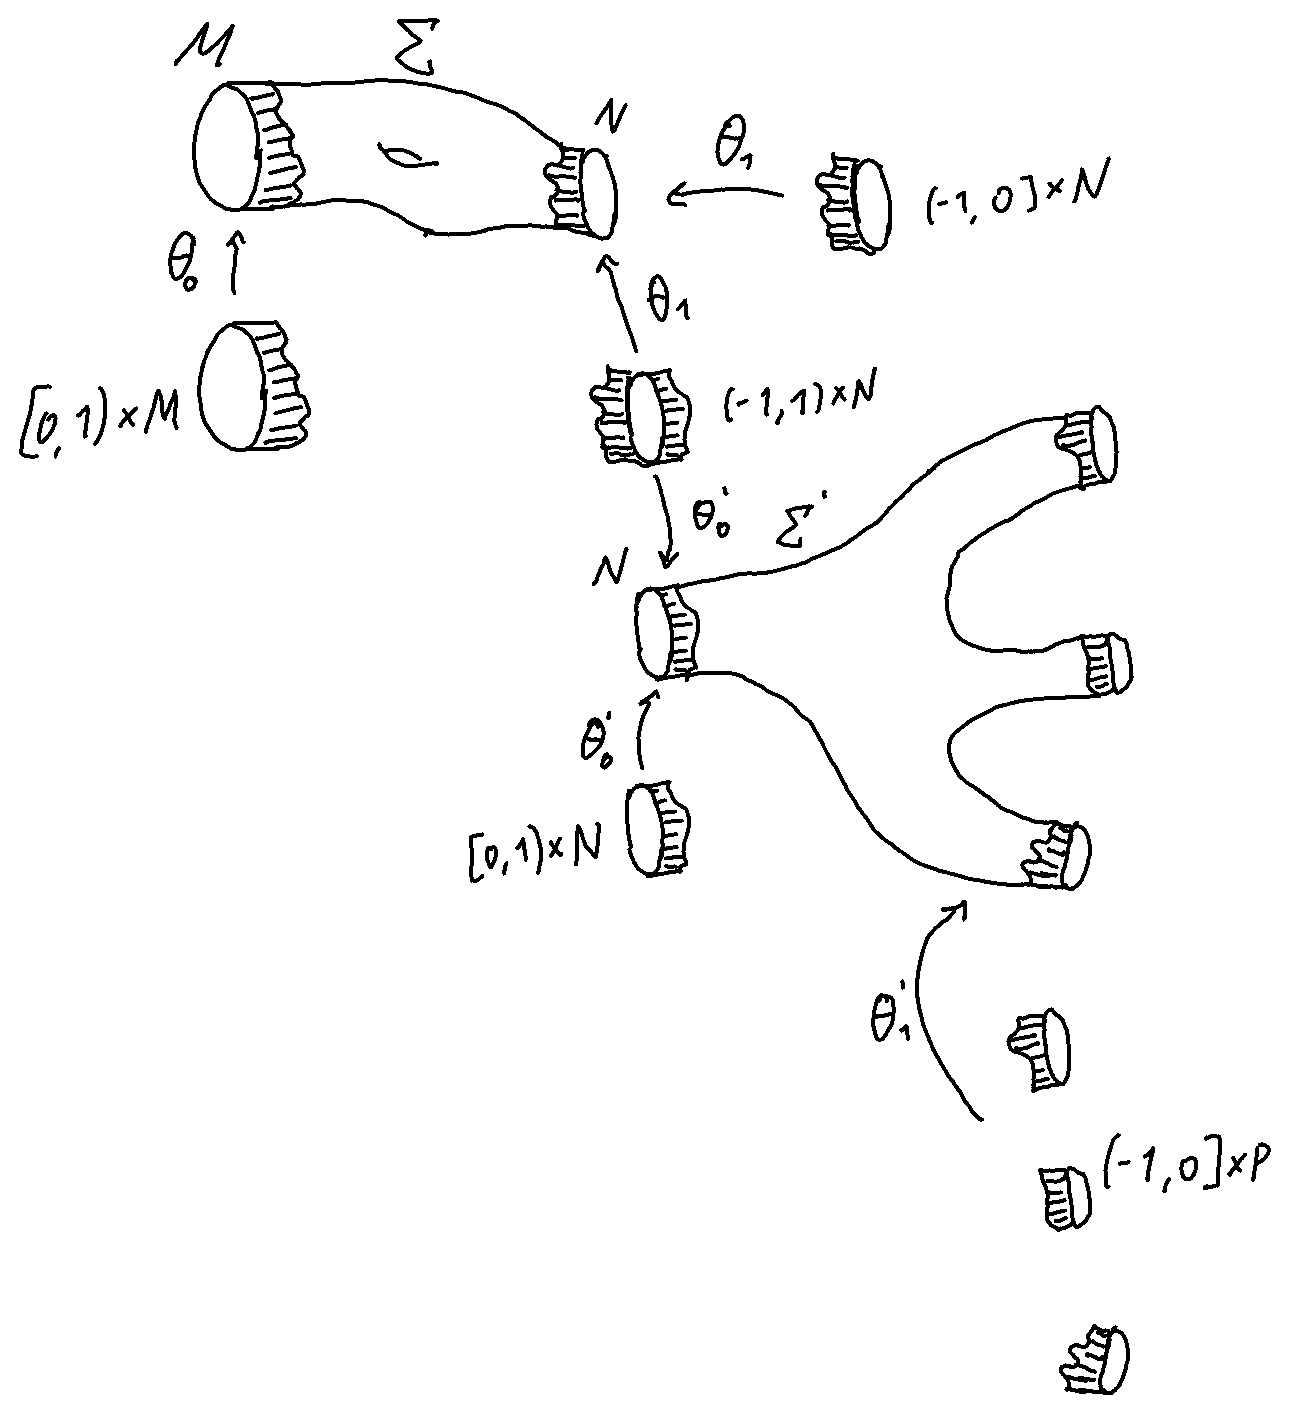
\includegraphics[width=70mm,scale=0.5]{images/Lecture 10/GlueBord.png}
         \caption{This is an illustration of gluing of two bordisms along their common boundary.}
         \label{Gluing Bordisms}
     \end{figure}
    The gluing of manifolds is associative. 
    In order for this to actually be a category there must be unital identity morphisms. For an object $M$ it is given by $M \times [0,1]$. 
    However, one could also take $M \times [0,2]$ which is diffeomorphic to $M \times [0,1]$ but \textit{not} strictly identical, on the nose. 
    That is why we took a \textit{diffeomorphism class} of bordisms. 
    In particular, the identity morphisms for any closed manifold $X\in\Bordn$, $X\xrightarrow{id_X}X$ is given by $[X\times [0,1]]_{_{\cong}}$ where $\cong$ denotes isomorphisms between smooth manifolds, i.e. diffeomorphisms.
\end{defn}
\begin{notat}
    $\nCob=\Bordn$, meaning that objects are closed $n-1$-dimensional manifolds and morphisms are diffeomorphism classes of bordisms. Moreover, we indicate that the closed manifolds are oriented and the bordisms orientation preserving with $\Bordnor$ or equivalently $\nCob^{\orient}$.
\end{notat}
Let us explicitly state what is meant by diffeomorphism of bordisms:
\begin{defn}
    A diffeomorphism of bordisms from $M$ to $N$, $(\Sigma, p, \theta_0, \theta_1) \to (\Sigma', p', \theta_0', \theta_1')$ is a diffeomorphism $\phi: \Sigma \to \Sigma'$ of manifolds with boundary 
    % https://q.uiver.app/#q=WzAsNCxbMSwwLCJNIl0sWzAsMSwiXFxTaWdtYSJdLFsyLDEsIlxcU2lnbWEnIl0sWzEsMiwiTiJdLFswLDEsIlxcdGhldGEoMCwtKSIsMix7InN0eWxlIjp7InRhaWwiOnsibmFtZSI6Imhvb2siLCJzaWRlIjoiYm90dG9tIn19fV0sWzEsMiwiXFxwaGkiLDJdLFsxLDIsIlxcY29uZyJdLFswLDIsIlxcdGhldGEnKDAsLSkiLDAseyJzdHlsZSI6eyJ0YWlsIjp7Im5hbWUiOiJob29rIiwic2lkZSI6ImJvdHRvbSJ9fX1dLFszLDEsIlxcdGhldGEoLSwxKSIsMCx7InN0eWxlIjp7InRhaWwiOnsibmFtZSI6Imhvb2siLCJzaWRlIjoiYm90dG9tIn19fV0sWzMsMiwiXFx0aGV0YScoLSwxKSIsMix7InN0eWxlIjp7InRhaWwiOnsibmFtZSI6Imhvb2siLCJzaWRlIjoidG9wIn19fV1d
\[\begin{tikzcd}
	& M \\
	\Sigma && {\Sigma'} \\
	& N
	\arrow["{\theta(0,-)}"', hook', from=1-2, to=2-1]
	\arrow["\phi"', from=2-1, to=2-3]
	\arrow["\cong", from=2-1, to=2-3]
	\arrow["{\theta'(0,-)}", hook', from=1-2, to=2-3]
	\arrow["{\theta(-,1)}", hook', from=3-2, to=2-1]
	\arrow["{\theta'(-,1)}"', hook, from=3-2, to=2-3]
\end{tikzcd}\]
    The commutativity of the latter diagram also implies that also extra data commute accordingly, e.g. with the partitions:
    % https://q.uiver.app/#q=WzAsMyxbMCwwLCJcXGRlXFxTaWdtYSJdLFsyLDAsIlxcZGVcXFNpZ21hJyJdLFsxLDEsIlxcezAsMVxcfSJdLFswLDEsIlxccGhpfF97XFxkZVxcU2lnbWF9Il0sWzAsMiwicCIsMl0sWzEsMiwicCciXV0=
\[\begin{tikzcd}
	\de\Sigma && {\de\Sigma'} \\
	& {\{0,1\}}
	\arrow["{\phi|_{\de\Sigma}}", from=1-1, to=1-3]
	\arrow["p"', from=1-1, to=2-2]
	\arrow["{p'}", from=1-3, to=2-2]
\end{tikzcd}\]
\end{defn}

\begin{ex}
    We have that 
        $$\Hom_{\nCob} (\emptyset, \emptyset) = \text{ \{closed $n$ manifolds\}}/\text{\{diffeomorphism\}}.$$
    For $n=2$, $\Sigma = S^2$ is a composition of
    %DRAWING

    while a genus $g$ surface is the composite:
    %DRAWING 

    which is very reminiscent of what we did in Morse theory. There we were actually also learning how the
     composition of bordisms works, this is called handle decomposition.
\end{ex}
We just saw that $\Bordn$ is a category. It has importantly also a symmetric monoidal structure:
\begin{itemize}
    \item (M) The tensor product is given by the disjoint union of manifolds, $\otimes = \amalg$, both on objects ($M \otimes N:= M \amalg N$) and on morphisms ($\Sigma \otimes \Sigma':= \Sigma \amalg \Sigma'$). Disjoint union is functorial since for $\Sigma:M\to N$, $\Sigma':M'\to N'$, $\Lambda:N\to P$, $\Lambda':N'\to P'$ in $\Bordn$ it holds that:
    \begin{itemize}
        \item $(\Sigma\cup_N\Lambda)\amalg(\Sigma'\cup_{N'}\Lambda')=(\Sigma\amalg\Sigma')\cup_{N\amalg N'}(\Lambda\amalg\Lambda')$
        \item $(M\xrightarrow{M\times[0,1]}M)\amalg(M'\xrightarrow{M'\times[0,1]}M')=M\amalg M'\xrightarrow{(M\times[0,1])\amalg (M'\times[0,1])}M\amalg M'$
        %A bit confused on how to actually check functoriality for the identity morphisms, please check if this makes sense /andrea
    \end{itemize}
    \item (O) $\unit_{\Bordn} = \emptyset$ (note that $\emptyset \amalg M \neq M$, so $\Bordn$ is not a \emph{strict} symmetric monoidal category\footnote{Note that objects were \textit{not} taken up to diffeomorphism, only morphisms.}. However, there is an isomorphism in the category since they're clearly diffeomorphic, and any diffeomorphic manifolds are cobordant. So, $\emptyset \amalg M \cong M$ in $\Bordn$, as we expect the monoidal unit to behave.
    \item (A) $M_1 \amalg (M_2 \amalg M_3) \xrightarrow{\cong} (M_1 \amalg M_2) \amalg M_3$ 
    \item (B) $\beta_{M,N}: M \amalg N \xrightarrow{\cong} N \amalg M$ and $\beta^2 = id$
\end{itemize}
\begin{rem}
    Associativity and commutativity also hold up to diffeomorphism and not strictly if one defines the disjoint union as a coproduct\footnote{A coproduct is the dual notion of (cartesian) product (see \ref{CartProd}), i.e. a coproduct in $\cat$ is a product in $\cat^{op}$.}: every coproduct is unique up to isomorphism\footnote{One can prove this in a specular way in which we proved the uniqueness of the cartesian product, see \ref{UptoIsoProds}.}, the appropriate notion of isomorphism in the category of smooth manifolds is diffeomorphism and all diffeomorphic manifolds are cobordant.
\end{rem}
\section{Definition of topological field theories}
Recall that a group homomorphism $\Omega_n \to X$ with $X$ also an abelian group is a bordism invariant, which is generally quite useful and interesting. Now that we have refined our tools and have a cobordism \emph{category} instead of the cobordism \emph{group}, the bordism invariants become symmetric monoidal functors into another symmetric monoidal category since symmetric monoidal functors are the appropriate notion of homomorphism of symmetric monoidal categories.

In particular, that's how we get a topological field theory:
\begin{defn}
    A topological field theory is a symmetric monoidal functor\footnote{See \ref{SymmMonFun} for the definition of symmetric monoidal functor.} with source $\nCob$ into a symmetric monoidal category $\cat$
    $$
        \Zf: \nCob \to \cat
    $$
\end{defn}


\begin{exercise}
\hfill
    \begin{itemize}
    \item Compare this definition to other definitions of quantum field theory.
    \item Skim through Atiyah's original paper \cite{Atiyah1988}, how does this definition compare to his set of axioms?
\end{itemize}
\end{exercise} 
After skimming through \cite{Atiyah1988} one might wonder why we defined the target category of a topological field to be just a general symmetric monoidal category and not specifically $(\Vect_{k},\otimes,k)$, as Atiyah did, or at least something similar, in the end we are studying topological quantum field theories! There are probably several reasons why someone would want to do so, for example for representation theoretic ones\footnote{e.g. \cite{stroppel2022categorification}, later we will also show that one must pick categories different to $\Vect_{k}$ in order to get interesting 3dTFTs and connect them with the Jones polynomial from knot theory.}. One of the crucial ones in particular is that one of the guiding conjectures of this field, the cobordism hypothesis, is formulated and provable without mentioning specifically $\Vect_{k}$ as a target category. See \ref{RemarkOnCobHypo} for more on this conjecture\footnote{As a spoiler: the moral of the cobordism hypothesis is that "The history of the Baez-Dolan conjecture \textit{[i.e. the cobordism hypothesis]} goes most directly through quantum field theory and its adaptation to low-dimensional topology. Yet in retrospect it is a theorem about the structure of manifolds in all dimensions..." \cite{freed2012cobordism} and hence TFTs are of interest with respect to any suitable target category, not only the ones of interest from the viewpoint of physics.}
\begin{rem}
    A TFT is a functor in a similar way that a linear representation of a group\footnote{
    In fact, some regard it a kind of representation, check out for instance around minute 18:00 of \hyperlink{https://www.youtube.com/watch?v=_9FxudwLWzg}{Catharina Stroppel: The beauty of braids - from knot invariants to higher categories}; 
    or the following quote from \hyperlink{https://www.hsm.uni-bonn.de/fileadmin/hsm/pictures/TQFT_Poster_01.pdf}{a poster for a conference on TQFTs and their connections to representation theory and mathematical physics} 
    "...a TQFT is a symmetric monoidal functor from the cobordism category to some symmetric monoidal category. It can thus be seen as a representation of a fundamental geometric category on a target category and thereby organizes interesting algebraic structures, e.g. representations of mapping class groups, in terms of cobordism categories. ..."; 
    or this quote from Daniel Freed "An extended topological field theory is a representation of the bordism category..." \cite{freed2012cobordism}.} is (see \ref{Representations of Groups}). 
    We can construct the category of TFTs in an analagous way to the one we used to define the category of linear representations of a group (see \ref{Cat of representations}): by constructing a functor category where the objects are TFTs (hence particular symmetric monoidal functors) and morphisms apt natural transformations between them\footnote{See \ref{SymmMonNat} for the definition of a symmetric monoidal natural transformation.}. 
    The category of $n$-dimensional TFTs will then be $\Hom_{\SymmMonCat}(\nCob,\cat)$ (see \ref{CatSymmMonCat} for the definition of $\SymmMonCat$, the category of all symmetric monoidal categories). 
    Similarly as with groups, one can have linear and non-linear representations, although linear representations appear more frequenly. 
    Typical examples of linear target categories are $(\AbGrp,\otimes),(\Mod_R,\otimes),(\Vect_k,\otimes)$.
\end{rem}

\begin{notat}[Category of TFTs]
    The category of TFTs is the functor category 
    $$\Hom_{\SymmMonCat}(\nCob,\cat)=\Fun^\otimes(\nCob,\cat)=\TFT_n(\cat)=\operatorname{nTFT}(\cat).$$ 
    This functor category is symmetric monoidal by defining the tensor product between TFTs pointwise: for $\Zf_1,\Zf_2\in\TFT_n(\cat)$ and $M\in\nCob$ $$(\Zf_1\otimes\Zf_2)(M):=\Zf_1(M)\otimes\Zf_2(M)$$
\end{notat}
TFTs were originally defined with Vect as the target category, $\Zf: (\nCob, \amalg) \to (\Vect, \otimes) $), see \cite{Atiyah1988}. In this case we can use the notation in equation \ref{eq:rep_of_cat} and write $\TFT_n(\Vect_k) = \Rep(\Bord_{n,n-1}$.
We can infer a few things about such TFTs:
\begin{enumerate}
    \item $\Sigma$ closed $n$ manifold, we can then view it as a bordism $\emptyset \xrightarrow{\Sigma} \emptyset$ and then we can apply $Z$ and we get $Z(\emptyset) \xrightarrow{Z(\Sigma)} Z(\emptyset)$ but $Z(\emptyset) = k$, since that's the unit in $\Vect$. So $\Zf(\Sigma)$ is a linear map from $k$ to $k$, which is entirely determined by where it sends one element. We then get that $\Zf(\Sigma)(\unit)$ is a diffeomorphism invariant.

    In fact, the original hope was to use TFTs to find new diffeomorphism invariants.
    \item There is a "trivial" TFT which on objects acts as $\Zf(M) = k$ and on morphisms as $\Zf(\Sigma) = id_k$ and we write $Z = 1$.
    \item An \emph{invertible} TFT is a TFT in which $Z(M) \cong k$ and $Z(\Sigma)$ is an isomorphism. Which is very similar but in the trivial TFT we have chosen not only $Z(M) \cong k$ but specifically $Z(M) = k$.
    This is related to "anomalies" in physics\footnote{To precisely see how, one needs to work with \emph{extended} TFTs, a higher categorical refinement of what we are working with now. See \cite{muller2020extended}.}.
\end{enumerate}

%TODO fix and write better, as in the exercises. Or maybe remove since it's in the exercises
\begin{ex}
    Euler characteristic ($\to$ Euler theory)

    \noindent Fix $\lambda \in \C^*$
    \begin{equation}
        Z_\lambda (\Sigma) := \lambda^{\chi(\Sigma)}, \quad Z(M) = \C
    \end{equation}
    Here functoriality follows from additivity
    \begin{equation}
        \chi(X \cup Y) = \chi(X) + \chi(Y) - \chi(X \cap Y)
    \end{equation}
\end{ex}


\begin{defn}\label{InvertibleObject}
    Let $(\cat, \otimes, \unit_\cat)$ be a monoidal category. An object $X \in \cat$ is invertible if there is a $Y \in \cat$ such that $X \otimes Y \cong \unit_\cat$.  
\end{defn}

\begin{ex}
    In $(\Vect_k, \otimes)$, $X$ is invertible iff there is a vector space $Y$ such that $X\otimes Y \cong k$.
\end{ex}

\begin{notat}
    $\cat^\times \subset \cat$ subset of invertible objects and isomorphisms. We will later see that this is the
     underlying Picard groupoid (see \ref{PicardDualizable}) %and synonymous with $(\cat^{dualizable})^{\cong}$
      %because of \ref{InvertibleDualizable}.
\end{notat}
%dim(X \otimes Y) =  dim(X)dim (Y) = dim X = 1....?
\begin{notat}
    For some symmetric monoidal category $(\cat,\otimes,\unit_\cat)$ we sometimes explicitly denote its tensor product by $\cat^\otimes$. For example, $\Set^\times$, $\Set^\amalg$, $\Vect^\oplus$, $\Vect^\otimes$.
\end{notat}

We can now rigorously define what we previously called an invertible TFT: 
\begin{defn}
    An invertible TFT is an invertible object in $\Fun^\otimes(\Bordn,\cat)$. This is equivalent to the fact that $\Zf$ factors through $\cat^\times$:
 % https://q.uiver.app/#q=WzAsMyxbMCwwLCJcXEJvcmRuXlxcYW1hbGciXSxbMiwwLCJcXGNhdF5cXG90aW1lcyJdLFsxLDEsIlxcY2F0XlxcdGltZXMiXSxbMCwxLCJcXFpmIl0sWzAsMiwiXFxiYXJ7XFxaZn0iLDIseyJzdHlsZSI6eyJib2R5Ijp7Im5hbWUiOiJkYXNoZWQifX19XSxbMiwxLCIiLDIseyJzdHlsZSI6eyJ0YWlsIjp7Im5hbWUiOiJob29rIiwic2lkZSI6InRvcCJ9fX1dXQ==
\[\begin{tikzcd}
	{\Bordn^\amalg} && {\cat^\otimes} \\
	& {\cat^\times}
	\arrow["\Zf", from=1-1, to=1-3]
	\arrow["{\bar{\Zf}}"', dashed, from=1-1, to=2-2]
	\arrow[hook, from=2-2, to=1-3]
\end{tikzcd}\]
\end{defn}
\begin{defn}[Groupoid Completion]
    Let $\cat$ be a category. A groupoid completion $(|\cat|,i)$ is a groupoid $|\cat|$ with a functor %Reminder: ask claudia hom of monoids in freed old new instead of functor
    $i:\cat\to|\cat|$ such that if $\dat$ is a groupoid and $f:\cat\to\dat$ a functor, then there is a unique map $\tilde{f}:|\cat|\to\dat$ such that the following diagram commutes 
    % https://q.uiver.app/#q=WzAsMyxbMCwwLCJcXGNhdCJdLFsyLDAsInxcXGNhdHwiXSxbMSwxLCJcXGRhdCJdLFswLDEsImkiXSxbMCwyLCJmIiwyXSxbMSwyLCJcXHRpbGRle2Z9IiwwLHsic3R5bGUiOnsiYm9keSI6eyJuYW1lIjoiZGFzaGVkIn19fV1d
\[\begin{tikzcd}[cramped]
	\cat && {|\cat|} \\
	& \dat
	\arrow["i", from=1-1, to=1-3]
	\arrow["f"', from=1-1, to=2-2]
	\arrow["{\tilde{f}}", dashed, from=1-3, to=2-2]
\end{tikzcd}\]
\end{defn}
From the universal property of the groupoid completion, there is a further factorization of an invertible field theory: 
% https://q.uiver.app/#q=WzAsNCxbMCwwLCJcXEJvcmRuXlxcYW1hbGciXSxbMiwwLCJcXGNhdF5cXG90aW1lcyJdLFsyLDEsIlxcY2F0XlxcdGltZXMiXSxbMCwxLCJ8XFxCb3Jkbl5cXGFtYWxnIl0sWzAsMSwiXFxaZiJdLFswLDIsIlxcYmFye1xcWmZ9IiwxXSxbMiwxLCIiLDIseyJzdHlsZSI6eyJ0YWlsIjp7Im5hbWUiOiJob29rIiwic2lkZSI6InRvcCJ9fX1dLFswLDMsImkiLDJdLFszLDIsIlxcdGlsZGV7XFxaZn0iLDJdXQ==
\[\begin{tikzcd}
	{\Bord^\amalg} && {\cat^\otimes} \\
	{|\Bord^\amalg}| && {\cat^\times}
	\arrow["\Zf", from=1-1, to=1-3]
	\arrow[hook, from=2-3, to=1-3]
	\arrow["i"', from=1-1, to=2-1]
	\arrow["{\tilde{\Zf}}"', from=2-1, to=2-3]
\end{tikzcd}\]
\begin{rem}
    Note that the groupoid completion of the bordism category $|\Bordn^\amalg|$ is a Picard groupoid, see \ref{PicardDualizable}.
\end{rem}
\begin{rem}
    A nTFT is invertible if the TFT is itself an invertible (see \ref{InvertibleObject}) object in the category of nTFTs.
\end{rem}

\subsection{Invertible field theories and stable homotopy theory \extra}\label{Spectra Phases of Matter}

These theories can be studied with stable homotopy theory. Stable homotopy homotopy theory is the branch
of homotopy theory that studies phenomena and structures that are stable under suspension. 
This is achieved via spectra. This begs the question: what are spectra?

\subsubsection{What are spectra? \extra}\label{WhatSpectra}
We already have seen some spectra and definitions of some kinds of spectra in \ref{homotopyCob}, e.g. the 
sphere spectrum and the suspension spectrum. In that section, we defined suspension as a quotient.
 However, one can define a suspension in full generality, i.e. for any pointed $\infty$-category, via certain homotopy
  colimits. Moreover, via such homotopy co/limits one can define other fundamental notions for spectra,
   so in what follows, we try to convey an idea for how they work.
  
   Homotopy co/limits are objects making certain diagrams commute via homotopies and with certain
   universal properties. Such diagrams commute in a very similar sense to how $\mathbb{E}_n$-algebras 
   are associative via homotopies of every order up to $\infty$. Every co/limit in an $\infty$-category works as a homotopy
   co/limit\footnote{Being able to define homotopy co/limits via usual universal properties is indeed one
   of the motivations for $\infty$-categories, as said in \ref{HomotopyHypothesis}.}, see \cite[Section
    4]{land2021introduction} for a thorough introduction to how that works.
    
    We now provide a rough sketch of what are homotopy co/limits. To do this, we first need to define 
    what are co/limits in ordinary categories.
       \begin{defn}[Terminal, initial, zero objects]
A terminal object in a category $\cat$ is an object $\ast\in\cat$ such that for every
$X\in\cat$ there is a unique morphism $X\to\ast$

An initial object in a category $\cat$ is an object $\emptyset\in\cat$ such that for every
$X\in\cat$ there is a unique morphism $\emptyset\to X$

A zero object is an object that is both initial and final. A category is called pointed if it has a zero object.
    \end{defn}
    
    \begin{defn}[Diagram]
    	Until now, we spoke of diagrams informally, there is however a precise definition. Given a
    	 small\footnote{This means that the collection of objects and morphisms are both sets}
    	category $\mathscr{J}$, a diagram of 
    	shape $\mathscr{J}$ in $\cat$ is a functor $D:\mathscr{J}\to \cat$
    \end{defn}
    \begin{defn}[Co/limits]
    	Given a category $\mathscr{J}$ we can construct 
    	\begin{itemize}
    		\item the cone\footnote{Aka left cone} of $\mathscr{J}$: $\mathscr{J}^{\lhd}$ by adding an initial object to $\mathscr{J}$
    		\item the cocone\footnote{Aka right cone} of $\mathscr{J}$: $\mathscr{J}^{\rhd}$ by adding a terminal object to $\mathscr{J}$
    	\end{itemize}
    	Given a diagram $D$ of shape $\mathscr{J}$ in $\cat$ and $X\in\cat$ we have 
    	
    	\begin{itemize}
    		\item a cone over $D$ that is a natural transformation $\gamma: X\Rightarrow D$, where $X$ denotes the functor sending every object in $\mathscr{J}$ to $X$. So, because of naturality
    		of $\gamma$ for $M\xrightarrow{f}N$ in $\mathscr{J}$ there is the following commutative diagram:
    	% https://q.uiver.app/#q=WzAsMyxbMSwwLCJYKE4pPVg9WChNKSJdLFswLDEsIkQoTikiXSxbMiwxLCJEKE0pIl0sWzAsMSwiXFxnYW1tYV97Tn0iLDJdLFswLDIsIlxcZ2FtbWFfe019Il0sWzEsMiwiRChmKSIsMl1d
    	\[\begin{tikzcd}[cramped]
    		& {X(N)=X=X(M)} \\
    		{D(N)} && {D(M)}
    		\arrow["{\gamma_{N}}"', from=1-2, to=2-1]
    		\arrow["{\gamma_{M}}", from=1-2, to=2-3]
    		\arrow["{D(f)}"', from=2-1, to=2-3]
    	\end{tikzcd}\]
    		We have then also the category of cones over $D$. 
    		An equivalent description of a cone over $D$ is a functor $\mathscr{J}^{\lhd}\to\cat$
    		hence the category of cones is the functor category
    		$\Fun_D(\mathscr{J}^{\lhd},\cat)$.
    		
    		\item a cocone over $D$ that is a natural transformation $\eta: D\Rightarrow X$ and because of naturality
    		of $\gamma$ for $M\xrightarrow{f}N$ in $\mathscr{J}$ there is the following commutative diagram:
    		% https://q.uiver.app/#q=WzAsMyxbMSwxLCJYKE4pPVg9WChNKSJdLFswLDAsIkQoTikiXSxbMiwwLCJEKE0pIl0sWzEsMCwiXFxldGFfe059IiwyXSxbMiwwLCJcXGV0YV97TX0iXSxbMSwyLCJEKGYpIl1d
    		\[\begin{tikzcd}[cramped]
    			{D(N)} && {D(M)} \\
    			& {X(N)=X=X(M)}
    			\arrow["{\eta_{N}}"', from=1-1, to=2-2]
    			\arrow["{\eta_{M}}", from=1-3, to=2-2]
    			\arrow["{D(f)}", from=1-1, to=1-3]
    		\end{tikzcd}\]
    		We have then also the category of cocones over $D$. An equivalent description of a cocone over $D$ is a functor $\mathscr{J}^{\rhd}\to\cat$
    		hence the category of cocones is the functor category
    		$\Fun_D(\mathscr{J}^{\rhd},\cat)$
    	\end{itemize}
    	Then, 
 \begin{itemize}
	\item the limit of the diagram $D$ is a terminal object in the category of cones over $\mathscr{J}$, i.e. $\Fun_D(\mathscr{J}^{\lhd},\cat)$
	\item the colimit of the diagram $D$ is an initial object in the category of cocones over $\mathscr{J}$, i.e. $\Fun_D(\mathscr{J}^{\rhd},\cat)$
\end{itemize}
In order to get a definition of homotopy co/limit or $(\infty,1)$-co/limit, just substitute your favourite
 model of $\infty$-category with 'category' in this definition. 
    \end{defn}
    \begin{ex}[Cartesian product]
 We previously defined the cartesian product of two objects by saying that some diagram commutes and the product  has a certain universal property (\ref{CartProd}). 
 Such cartesian product is a limit over a diagram shaped as a discrete category with two objects.
 Let us name this discrete category with two different objects $\mathscr{J}=\{0,1\}$, discrete means that
 there are only the identity morphisms $id_0$ and $id_1$. 
 Given $\cat$ an arbitrary category, observe a diagram 
 $$D:\mathscr{J}\to \cat $$ 
 $$0\mapsto A$$
 $$1\mapsto B$$
 Then, a cartesian product $A\times B$ is the limit over $D$
    % https://q.uiver.app/#q=WzAsNSxbMSwwLCJZIl0sWzIsMSwiQiJdLFswLDBdLFswLDEsIkEiXSxbMSwxLCJBXFx0aW1lcyBCIl0sWzAsMSwiZyJdLFs0LDMsInByXzEiXSxbMCwzLCJmIiwyXSxbNCwxLCJwcl8yIiwyXSxbMCw0LCJcXGV4aXN0cyEgdSIsMSx7InN0eWxlIjp7ImJvZHkiOnsibmFtZSI6ImRhc2hlZCJ9fX1dXQ==
\[\begin{tikzcd}
	{} & Y \\
	A & {A\times B} & B
	\arrow["g", from=1-2, to=2-3]
	\arrow["{pr_1}", from=2-2, to=2-1]
	\arrow["f"', from=1-2, to=2-1]
	\arrow["{pr_2}"', from=2-2, to=2-3]
	\arrow["{\exists! u}"{description}, dashed, from=1-2, to=2-2]
\end{tikzcd}\]
The two projections exist because $A\times B$ is a cone: a cone is an initial object in the shape category $\mathscr{J}$ and $D$ is a functor, so it imports the unique morphisms from the initial object to where $0$ and $1$ are mapped, i.e. to $A$ and $B$.

\noindent $u$ exists and is unique because $A\times B$ is the terminal object in the category of cones.

 \noindent The two smaller triangles commute because of the naturality of the morphism $u$: recall that
 the category of cones is a functor category hence morphisms between cones 
 are natural transformations and note that $pr_1$ and $f$ for instance are images of morphisms in
  $\mathscr{J}^{\lhd}$
    \end{ex}
    We already sketched what might mean that a diagram is homotopy coherently commutative in the
     case of an $\mathbb{E}_1$-algebra (\ref{EAlg}). For the sake of clarity we sketch it here again,
     in a more general setting. Recall that all morphisms higher than 1 in an $\infty$-category are weakly invertible.
% https://q.uiver.app/#q=WzAsNSxbMCwwLCJBIl0sWzAsMiwiQiJdLFsyLDIsIkQiXSxbMiwwLCJDIl0sWzEsMSwiLi4uIl0sWzAsMywiZyJdLFswLDEsImYiLDJdLFsxLDIsInEiLDJdLFszLDIsInIiXSxbMSwzLCJoIiwwLHsiY3VydmUiOi0zLCJzaG9ydGVuIjp7InNvdXJjZSI6MTAsInRhcmdldCI6MTB9LCJsZXZlbCI6Mn1dLFszLDEsImsiLDAseyJjdXJ2ZSI6LTMsInNob3J0ZW4iOnsic291cmNlIjoxMCwidGFyZ2V0IjoxMH0sImxldmVsIjoyfV0sWzksMTAsIm0iLDIseyJjdXJ2ZSI6Mywic2hvcnRlbiI6eyJzb3VyY2UiOjIwLCJ0YXJnZXQiOjIwfX1dLFsxMCw5LCJsIiwyLHsiY3VydmUiOjMsInNob3J0ZW4iOnsic291cmNlIjoyMCwidGFyZ2V0IjoyMH19XV0=
\[\begin{tikzcd}[cramped]
	A && C \\
	& {...} \\
	B && D
	\arrow["g", from=1-1, to=1-3]
	\arrow["f"', from=1-1, to=3-1]
	\arrow["q"', from=3-1, to=3-3]
	\arrow["r", from=1-3, to=3-3]
	\arrow[""{name=0, anchor=center, inner sep=0}, "h", curve={height=-18pt}, shorten <=7pt, shorten >=7pt, Rightarrow, from=3-1, to=1-3]
	\arrow[""{name=1, anchor=center, inner sep=0}, "k", curve={height=-18pt}, shorten <=7pt, shorten >=7pt, Rightarrow, from=1-3, to=3-1]
	\arrow["m"', curve={height=18pt}, shorten <=8pt, shorten >=8pt, Rightarrow, from=0, to=1]
	\arrow["l"', curve={height=18pt}, shorten <=8pt, shorten >=8pt, Rightarrow, from=1, to=0]
\end{tikzcd}\]
     This diagram does not commute strictly, but via homotopies.
     This means that $h:q\circ f\simeq r\circ g:k$, instead of what we are used to: $q\circ f= r\circ g$.
     Not only this however, it is the case that $k\circ h\simeq id_{q\circ f}$ and $h\circ k\simeq id_{r\circ g}$
     , instead of the usual strict invertibility, and thus via the 3-morphisms $l$ and $m$, the 2-morphisms 
     $k$ and $h$ are homotopic, i.e. $l:k\simeq h:m$. Then there
     will be some explicit 4-morphisms witnessing that $m\simeq l$, and so on to $\infty$.
    
   %I am unsure about the sketch above!!!! Please check /Andrea
   
      
   \begin{ex}[Homotopy pullback/$(\infty,1)$-pullback]
   	Let  $\mathscr{J}$ be an $\infty$-category with objects and 1-morphisms $0\to1\leftarrow2$ and
   	 $D:\mathscr{J}\to \cat$ be a diagram. To be rigorous, we would need to define what is an
   	 $\infty$-functor. However, since this necessitates getting our hands dirty with a model,
   	 we prefer to remain loose: an $\infty$-functor is an assignment that respects composition and identity
   	  morphisms\footnote{i.e. is functorial.} not only on 1-morphisms, but for also all higher invertible morphisms.
   	  Then, an $\infty$-pullback of 
   	is the homotopy limit of $D$.
   	
   	We now unpack what this means. A cone of $\mathscr{J}$, where $\emptyset$ is the new initial object
   	 looks like this:
   	% https://q.uiver.app/#q=WzAsNCxbMCwwLCJcXGVtcHR5c2V0Il0sWzAsMSwiMCJdLFsxLDEsIjEiXSxbMSwwLCIyIl0sWzAsMV0sWzEsMl0sWzAsM10sWzMsMl0sWzAsMl0sWzgsMSwiIiwxLHsic2hvcnRlbiI6eyJzb3VyY2UiOjIwfSwic3R5bGUiOnsidGFpbCI6eyJuYW1lIjoiYXJyb3doZWFkIn19fV0sWzgsMywiIiwxLHsic2hvcnRlbiI6eyJzb3VyY2UiOjIwfSwic3R5bGUiOnsidGFpbCI6eyJuYW1lIjoiYXJyb3doZWFkIn19fV1d
   	\[\begin{tikzcd}[cramped]
   		\emptyset & 2 \\
   		0 & 1
   		\arrow[from=1-1, to=2-1]
   		\arrow[from=2-1, to=2-2]
   		\arrow[from=1-1, to=1-2]
   		\arrow[from=1-2, to=2-2]
   		\arrow[""{name=0, anchor=center, inner sep=0}, from=1-1, to=2-2]
   		\arrow[shorten <=2pt, Rightarrow, 2tail reversed, from=0, to=2-1]
   		\arrow[shorten <=2pt, Rightarrow, 2tail reversed, from=0, to=1-2]
   	\end{tikzcd}\]
   	Where the two small triangles commute via higher morphisms denoted with $\Leftrightarrow$.
   	
   	Let $D(1)=X$, $D(2)=Y$ and $D(0)=Z$. Then, the $\infty$-pullback of $D$ is the terminal object 
   	in the $\infty$-functor $\infty$-category $\Fun_D(\mathscr{J},\cat)$. Denote the image of $\emptyset$ of such pullback with $Y\times_X Z$. Then there is the following homotopy coherent diagram
   % https://q.uiver.app/#q=WzAsNCxbMCwwLCJZXFx0aW1lc19YIFoiXSxbMCwxLCJZIl0sWzEsMSwiWiJdLFsxLDAsIlgiXSxbMCwxXSxbMSwyXSxbMCwzXSxbMywyXSxbMCwyXSxbOCwxLCIiLDEseyJzaG9ydGVuIjp7InNvdXJjZSI6MzAsInRhcmdldCI6MTB9LCJzdHlsZSI6eyJ0YWlsIjp7Im5hbWUiOiJhcnJvd2hlYWQifX19XSxbOCwzLCIiLDEseyJzaG9ydGVuIjp7InNvdXJjZSI6MzAsInRhcmdldCI6MTB9LCJzdHlsZSI6eyJ0YWlsIjp7Im5hbWUiOiJhcnJvd2hlYWQifX19XV0=
   \[\begin{tikzcd}[cramped]
   	{Y\times_X Z} & X \\
   	Y & Z
   	\arrow[from=1-1, to=2-1]
   	\arrow[from=2-1, to=2-2]
   	\arrow[from=1-1, to=1-2]
   	\arrow[from=1-2, to=2-2]
   	\arrow[""{name=0, anchor=center, inner sep=0}, from=1-1, to=2-2]
   	\arrow[shorten <=4pt, shorten >=1pt, Rightarrow, 2tail reversed, from=0, to=2-1]
   	\arrow[shorten <=4pt, shorten >=1pt, Rightarrow, 2tail reversed, from=0, to=1-2]
   \end{tikzcd}\]
   	Because the $\infty$-pullback is a functor and thus preserves the homotopy-coherent commutativity
   	of diagrams in the shape $\mathscr{J}$, by preserving compositionality for all $n$-morphisms.
   	Since it is the terminal object in the category of cones over the diagram $D$ for every other cone
   	mapping $\emptyset$ to an object $Q\in\cat$, then there is a unique morphism $Q\to Y\times_X Z$
   	making the following diagram commute homotopy coherently
   	
   	% https://q.uiver.app/#q=WzAsNSxbMSwxLCJZXFx0aW1lc19YIFoiXSxbMSwyLCJZIl0sWzIsMiwiWiJdLFsyLDEsIlgiXSxbMCwwLCJRIl0sWzAsMV0sWzEsMl0sWzAsM10sWzMsMl0sWzAsMl0sWzQsMF0sWzQsMV0sWzQsM10sWzksMSwiIiwxLHsic2hvcnRlbiI6eyJzb3VyY2UiOjMwLCJ0YXJnZXQiOjEwfSwic3R5bGUiOnsidGFpbCI6eyJuYW1lIjoiYXJyb3doZWFkIn19fV0sWzksMywiIiwxLHsic2hvcnRlbiI6eyJzb3VyY2UiOjMwLCJ0YXJnZXQiOjEwfSwic3R5bGUiOnsidGFpbCI6eyJuYW1lIjoiYXJyb3doZWFkIn19fV0sWzEwLDExLCIiLDAseyJzaG9ydGVuIjp7InNvdXJjZSI6MjAsInRhcmdldCI6MjB9LCJzdHlsZSI6eyJ0YWlsIjp7Im5hbWUiOiJhcnJvd2hlYWQifX19XSxbMTAsMTIsIiIsMix7InNob3J0ZW4iOnsic291cmNlIjoyMCwidGFyZ2V0IjoyMH0sInN0eWxlIjp7InRhaWwiOnsibmFtZSI6ImFycm93aGVhZCJ9fX1dXQ==
   	\[\begin{tikzcd}[cramped]
   		Q \\
   		& {Y\times_X Z} & X \\
   		& Y & Z
   		\arrow[from=2-2, to=3-2]
   		\arrow[from=3-2, to=3-3]
   		\arrow[from=2-2, to=2-3]
   		\arrow[from=2-3, to=3-3]
   		\arrow[""{name=0, anchor=center, inner sep=0}, from=2-2, to=3-3]
   		\arrow[""{name=1, anchor=center, inner sep=0}, from=1-1, to=2-2]
   		\arrow[""{name=2, anchor=center, inner sep=0}, from=1-1, to=3-2]
   		\arrow[""{name=3, anchor=center, inner sep=0}, from=1-1, to=2-3]
   		\arrow[shorten <=4pt, shorten >=1pt, Rightarrow, 2tail reversed, from=0, to=3-2]
   		\arrow[shorten <=4pt, shorten >=1pt, Rightarrow, 2tail reversed, from=0, to=2-3]
   		\arrow[shorten <=2pt, shorten >=2pt, Rightarrow, 2tail reversed, from=1, to=2]
   		\arrow[shorten <=4pt, shorten >=4pt, Rightarrow, 2tail reversed, from=1, to=3]
   	\end{tikzcd}\]
   	The two small triangles formed by morphisms that have $Q$ as source and by the projections of $Y\times_X Z$ (the ones on the upper left) commute because of the naturality of morphisms in 
   	 $\Fun_D(\mathscr{J}^{\lhd},\cat)$
   \end{ex}
 \begin{notat}
From now on, when we are talking about commutative diagrams in an $\infty$-category, we do not write the double arrows $\Leftrightarrow$ symbolizing the 
higher morphisms that make the diagram commute.
 \end{notat}
   

   
   There is the dual notion of homotopy pullback: the homotopy pushout, which we now use to define
    suspensions.

    \begin{defn}[Suspension]
   	Let $\cat$ be a pointed\footnote{A category with a zero object: an object that is both initial and final.} 
   	 $\infty$-category with the zero object denoted by 0 
   	 and let $X\in\cat$. Then the suspension $\Sigma X$ of $X$ is the pushout 
  % https://q.uiver.app/#q=WzAsNCxbMCwwLCJYIl0sWzAsMSwiMCJdLFsxLDAsIjAiXSxbMSwxLCJcXFNpZ21hIFgiXSxbMCwxXSxbMCwyXSxbMSwzXSxbMiwzXSxbMywwLCIiLDEseyJzdHlsZSI6eyJuYW1lIjoiY29ybmVyIn19XV0=
  \[\begin{tikzcd}[cramped]
  	X & 0 \\
  	0 & {\Sigma X}
  	\arrow[from=1-1, to=2-1]
  	\arrow[from=1-1, to=1-2]
  	\arrow[from=2-1, to=2-2]
  	\arrow[from=1-2, to=2-2]
  	\arrow["\lrcorner"{anchor=center, pos=0.125, rotate=180}, draw=none, from=2-2, to=1-1]
  \end{tikzcd}\]
   \end{defn}

   \begin{defn}[Suspension functor]
Given a pointed $\infty$-category $\cat$ the assignment $X\mapsto \Sigma X$ gives rise to a functor $\Sigma:\cat\to\cat$
   \end{defn}
   Dually, one can define the loop space of an object
\begin{defn}[Loop space]
   	Let $\cat$ be a pointed
$\infty$-category and let $X\in\cat$. Then the loop space $\Omega X$ is the pullback 
% https://q.uiver.app/#q=WzAsNCxbMCwwLCJcXE9tZWdhIFgiXSxbMCwxLCIwIl0sWzEsMCwiMCJdLFsxLDEsIlgiXSxbMCwxXSxbMCwyXSxbMSwzXSxbMiwzXSxbMCwzLCIiLDEseyJzdHlsZSI6eyJuYW1lIjoiY29ybmVyIn19XV0=
\[\begin{tikzcd}[cramped]
	{\Omega X} & 0 \\
	0 & X
	\arrow[from=1-1, to=2-1]
	\arrow[from=1-1, to=1-2]
	\arrow[from=2-1, to=2-2]
	\arrow[from=1-2, to=2-2]
	\arrow["\lrcorner"{anchor=center, pos=0.125}, draw=none, from=1-1, to=2-2]
\end{tikzcd}\]
\end{defn}
\begin{defn}[Loop space functor]
	Given a pointed $\infty$-category $\cat$ the assignment $X\mapsto \Omega X$ gives rise to a functor $\Omega:\cat\to\cat$
\end{defn}
\begin{rem}
	As already mentioned in \ref{EAlg}, a loop space is an example of $\mathbb{E}_1$-space and 
	$n$-iterated loop spaces are $\mathbb{E}_n$-spaces by the Dunn additivity theorem.
\end{rem}
\begin{defn}[Alternative definition of adjunction]\label{HigherAdjFun}
We defined adjoint functors via the natural tranformations unit and counit (\ref{AdjFun}). There is however an equivalent
formulation:
two $\infty$-functors $\cat\underset{L}{\overset{R}{\leftrightarrows}}\dat$ form an adjunction $L\dashv R$, i.e. where $L$ is the left adjoint
and $R$ is the right adjoint, if between the two Hom-$\infty$-functors 
$$\Hom_\cat(L(-),-):\cat^{\operatorname{op}}\times\cat \to \operatorname{Grpd}_\infty$$
and
$$\Hom_\dat(-,R(-)):\dat^{\operatorname{op}}\times\dat\to \operatorname{Grpd}_\infty$$
there is a natural isomorphism $\Hom_\cat(L(-),-)\simeq \Hom_\dat(-,R(-))$

This definition is easily derivable from the one with units we gave previously, given 
the unit $\epsilon:id_{\dat}\Rightarrow R\circ L$ and $X\in\cat$ and $Y\in\dat$, 
the following holds because of one of the triangle identities: 
% https://q.uiver.app/#q=WzAsMyxbMCwwLCJcXEhvbV97XFxjYXR9KEwoWSksWCkiXSxbMSwxLCJcXEhvbV9cXGRhdChSKEwoWSkpLFIoWCkpIl0sWzIsMCwiXFxIb21fXFxkYXQoWSxSKFgpKSJdLFswLDFdLFsxLDJdLFswLDIsIlxcc2ltZXEiXV0=
\[\begin{tikzcd}[cramped]
	{\Hom_{\cat}(L(Y),X)} && {\Hom_\dat(Y,R(X))} \\
	& {\Hom_\dat(R(L(Y)),R(X))}
	\arrow[from=1-1, to=2-2]
	\arrow[from=2-2, to=1-3]
	\arrow["\simeq", from=1-1, to=1-3]
\end{tikzcd}\]
\end{defn}
\begin{rem}[Suspension-loop adjunction]
There is an adjunction $\Sigma\dashv\Omega$ and thus for any pointed $\infty$-category
$\cat$ it holds that $\Hom_{\cat}(\Sigma-,-)\simeq \Hom_{\cat}(-,\Omega-)$. If it is not sufficiently clear from
the fact that 
$\Omega X=0\times_X 0$ and $\Sigma X=0\amalg_X 0$, do not worry. In the case that it interests us the most
it can be seen from another perspective. Recall that for $X\in \Top_\ast$
$\Sigma X= X\land S^1$ and $\Omega_x=\operatorname{Map}_{\ast}(S^1,X)$ and that $\Top_\ast$ is cartesian
 monoidal closed, i.e. for any $A,B,C\in\Top_\ast$ it holds that $\Hom_{\Top_{\ast}}(A\land B, C)\cong\Hom_{\Top_{\ast}}(A,\operatorname{Map}_{\ast}(B,C))$ and hence 
 $\Hom_{\Top_{\ast}}(-\land S^1,-)\cong\Hom_{\Top_{\ast}}(-,\operatorname{Map}_{\ast}(S^1,-))$
\end{rem}
\begin{defn}[Spectrum\footnote{Also denoted $\Omega$-spectrum in the older literature, e.g. books or 
	articles by May.}]
	A spectrum is a collection of 
	pointed spaces $\{E_n\}_{n\in\Z}$ with equivalences $\delta_n:E_n\simeq \Omega E_{n+1}$
\end{defn}
\begin{rem}
Note that via the adjunction $\Sigma\dashv\Omega$ we can get a sequential spectrum from a spectrum:
given $X_i,X_{i+1}\in\sat_\ast$ it holds that 
$\Hom_{\sat_{\ast}}(X_i,\Omega X_{i+1})\simeq \Hom_{\sat_{\ast}}(\Sigma X_i,X_{i+1})$ and thus we can 
get the pointed maps we need in order to define a sequential spectrum. This means that every spectrum
is a sequential spectrum, i.e. the category of spectra is a subcategory of the category of sequential spectra.


\end{rem}
\begin{defn}[$\infty$-category of spectra]
The $\infty$-category of spectra is the category where objects are spectra. %The fact that there
%are equivalences $X_i\simeq\Omega X_{i+1}$ 


This is equivalent to saying that the category of spectra is the sequential homotopy limit 
$$\operatorname{lim}(...\leftarrow\sat_\ast\leftarrow\sat_\ast\leftarrow\sat_\ast\leftarrow ...)$$
where we can see the diagram we are taking the limit over as a functor 
$D:\Z^{\operatorname{op}}\to\infty\operatorname{-Cat}$ where $\Z$ is considered as a category
via its ordering ($\leq$ corresponds to a morphism $\to$) and for each $i\in\Z$ $D(i)=\sat_\ast$. %Sometimes 
%such diagrams are called towers. %TBD
\end{defn}
The initial object of such category is the sphere spectrum $\mathds{S}$.
\begin{defn}[Infinite loop space]\label{InfiniteLoop}
	An infinite loop space is a space $X_0$ with an infinite sequence of pointed spaces $X_0,X_1,X_2,...$ with weak equivalences for $n\geq 0$
	 $$X_n\simeq \Omega X_{n+1}$$
	
	 %\footnote{The loop space object is an inverse operation to the delooping, meaning that that given some monoidal category $\cat$, $\cat$ is the loop space object of the delooping of $\cat$. The name comes from the topological notion, see \url{https://en.wikipedia.org/wiki/Loop_space}
		
		%In general, loop space objects inherit the monoidal structure from the composition of loops. We would need to talk about homotopy pullbacks in order to strictly define what a loop space object is.}

\end{defn}
\begin{rem}[Important observation: Infinite loop spaces=grouplike $\E_\infty$-spaces=Picard groupoids]\label{InfLoopsPicard}
We already argued in \ref{EAlg} that such infinite loop spaces are grouplike
$\mathbb{E}_\infty$-spaces because of the Dunn additivity theorem \ref{DunnAdds}.
Moreover, also in \ref{EAlg} we explained how grouplike
$\mathbb{E}_\infty$-spaces are
Picard $\infty$-groupoids:\begin{itemize}
\item the $\E_\infty$ makes them homotopy coherent commutative
monoid objects in $\operatorname{Grpd}_\infty$, i.e. symmetric monoidal $\infty$-groupoids
\item since they are grouplike, they have inverses because if we first
apply $\pi_0$, then forget about the commutative structure, and land in the category of groups, that
means that the inverses must have been there from the start
\end{itemize} 
\end{rem}


Infinite loop spaces seem very similar to what we defined as spectra. However, there is a crucial 
difference: there is no space to start from in a spectrum, since there are deloopings for all spaces, i.e. $ X_{-1}\simeq \Omega X_{0}$, 
$ X_{-2}\simeq \Omega X_{-1}$ and so on, while in an infinite loop space there are not.
\begin{defn}[Underlying (infinite loop) space functor]
	Given a spectrum, the assignment of a spectrum $ \{X_i\}_{i\in\Z}$ to its underlying
	infinite loop space, aka 0-th space, is a functor.
	$$\Omega^{\infty}:\operatorname{Sp}\to\sat_\ast$$	
	$$ \{X_i\}_{i\in\Z}\mapsto X_0$$
\end{defn}
Such assignment has a left adjoint.
\begin{defn}[Suspension spectrum functor]
$$\Sigma^{\infty}:\sat_\ast\to\operatorname{Sp}$$
\end{defn}
\begin{defn}[Classifying spectrum]
	Let $M$ be an $\mathbb{E}_\infty$-space, i.e. an $\mathbb{E}_\infty$-algebra in $\sat_\ast$ (see
	 \ref{EAlg}). Then we define the classifying spectrum of $M$
$$\mathbf{B}^{\infty}(M):=$$
\end{defn}
\begin{defn}[Classifying spectrum functor]
$$\mathbf{B}^{\infty}$$
\end{defn}
Picard $\infty$-groupoids do not only correspond to infinite loop spaces but also to connective 
spectra. 
\begin{thm}[Recognition theorem for infinite loop spaces, Boardman-Vogt, May]\label{RecognitionInfLoops}
	There is an equivalence: 
	$$\mathbf{B}^{\infty}:\Alg_{\mathbb{E}_{\infty}}^{\operatorname{gp}}(\mathscr{S})\leftrightarrows\operatorname{Sp}_{\geq 0}:\Omega^{\infty}$$
	where $\operatorname{Sp}_{\geq 0}$ denotes the category of connective spectra.
\end{thm}
\begin{proof}
	%TBD
\end{proof}
For a detailed proof see \cite[Corollary II.24]{KtheoryHebestreitWagner}. 

The natural question now is what kind of spectra are connective spectra? We now sketchily characterize them.

While the degree homotopy groups for usual topological spaces are defined to be positive, homotopy groups of spectra can be defined and be non-trivial also for negative degrees. Connective spectra are spectra that only have positive non-trivial homotopy groups. They
are called connective because a synonym is ($-1$)-connected spectra, referring to the convention that an $n$-connected space is a space where its homotopy groups for all $k\leq n$ are trivial. 

In sum, spectra are a higher categorical analog of abelian groups (see \ref{Ab-Enriched Cat}), they have been in fact called “the abelian groups of the 21st century” \cite{Mazel-Gee2024}
because they provide very powerful techniques for many areas of mathematics
where there is currently much progress, e.g. in algebraic K-theory. One can do algebra with 
spectra as one does ordinary algebra with abelian groups and rings, this subject is usually called 
'higher algebra'\footnote{A
	funny synonym for higher algebra is brave new algebra, referring to Huxley's dystopian
	novel \textit{Brave New World}. It was coined by Waldhausen, one of
	the pioneers of this discipline, hinting at the fact that it seems to have myriads of intriguing
	opportunities but at the same could lead into a world of pure abstractions detached from mathematics
	 with actual content. Examples of successful applications of such machinery
	to concrete problems, e.g. the counterexamples to Ravenel's telescope conjecture
	\cite{burklund2023ktheoretic}, convince the author of this section that this nightmare was avoided,
	 although 
	it must be said that they are clearly biased.}. This is not just a vague analogy, 
but something that can be motivated formally, for instance, abelian groups are discrete spectra:
 $$\pi_0:\operatorname{Sp}\to\operatorname{Ab}$$
 where in particular $\pi_0(\mathds{S})=\Z$
 %In a certain sense, $\mathds{S}$ is analgous to $\Z$ but in another category: \Z is the unit in Ab, while $\mathds{S}$ is the unit in the category of spectra. 

We make the comparison clearer via the following table\footnote{his table was inspired by a table in Thomas
	Nikolaus' talk: \url{https://www.youtube.com/watch?v=SJNKs1PxT9g}. } :

\begin{center}
	\begin{tabular}{||c|c||}
		\hline
		algebra & higher algebra\\ [0.5ex]
		\hline\hline
		set & $\infty$-groupoid\\
		\hline
		abelian group & spectrum \\
		\hline
		Ab & Sp \\
		\hline
		\Z &  $\mathds{S}$ \\
		\hline
		ring & $\E_1$-ring spectrum \\
		\hline
		commutative ring & $\mathbb{E}_\infty$-ring spectrum \\
		\hline
		Ab-enriched category & Sp-enriched category \\
		\hline
		abelian category & stable category \\
		\hline
	\end{tabular}
\end{center}
See \ref{Ab-Enriched Cat} and \ref{AbelianCat} for the definitions of Ab-enriched category and
abelian category. See \ref{EAlg} for the definitions of $\E_1$-ring spectrum and of
 $\mathbb{E}_\infty$-ring spectrum. A stable
 category is a category where $\Sigma\dashv\Omega$ do not just form an adjunction, but are equivalent. 
 There is an equivalent definition of stable category that more closely resembles the definition of abelian
  category, see \cite[Section 1]{Luriealgebra}.

\subsubsection{Invertible field theories are maps of spectra \extra}
 In order to allow the application of stable homotopy theory, one must fully extend topological field theories (see \ref{RemarkExtendedTFTs}), i.e. with $(\infty,n)$-categories of bordisms as a source, because
 only with the homotopy coherent additional structure of such categories one gets that $|\Bord|$ and
  $\cat^\times$ are particular kinds of spectra.
  
  In the case of extended TFTs, $|\Bord|$ and $\cat^\times$ both are $\infty$-groupoids since
\begin{enumerate}
	\item we get $|\Bord|$ by adjoining all inverses for all morphisms and thus all morphisms become invertible
	\item  $\cat^\times$ is obtained by forgetting about non-invertible morphisms (and objects) of $\cat$ and thus we are left only with invertible morphisms
\end{enumerate} 

%We previously talked about the fundamental $\infty$-groupoid of a space while sketching the
 %homotopy hypothesis (see \ref{HomotopyHypothesis}) and told a story about how spaces are
 %equivalent to $\infty$-groupoids. Following this line of thinking, $\tilde\Zf$ corresponds to a
 %map of spaces via this equivalence.

However, we do not have just $\infty$-groupoids but also a symmetric monoidal structure with
 duals on both $|\Bord|$ and $\cat^\times$. In short, they are Picard $\infty$-groupoid. Thanks to 
 \ref{InfLoopsPicard}, we know that they are thereby grouplike $\E_n$-spaces and infinite loop spaces.
  Via the recognition
 principle for infinite loop spaces \ref{RecognitionInfLoops}, we know that they are connective spectra.
 
 This is why $\tilde\Zf$ is not just a map of spaces but a map of spectra, and this enables the application of stable homotopy theory, making life easier. We can conclude this interlude on stable homotopy theory and invertible TFTs with the following motto
$$\text{\textit{Invertible TFTs are maps of connective spectra!}}$$
This is not only of theoretical interest but it also allows the application of topological field theories to condensed matter theory! Classical phases of matter are governed by Landau
 theory of phase transition. However, the phases of a quantum material do not behave in the
  same manner. Fortunately, there are ways to describe them, or at least specific types of quantum matter (with gapped Hamiltonians for instance)\footnote{Kitaev for instance proposed in \cite{Kitaev_2009} that the topological insulators and superconductors of a certain type of condensed matter are classifiable via K-theory\footnote{See \url{https://ncatlab.org/nlab/show/topological+phase+of+matter} and \url{https://ncatlab.org/nlab/show/K-theory+classification+of+topological+phases+of+matter}.} and this was further refined via twisted equivariant K-theory by Dan Freed and Greg Moore in \cite{Freed_2013}. }. The topological field theories describing the (\href{https://ncatlab.org/nlab/show/topological+phase+of+matter}{topological}) phases of matter of some condensed matter systems (with short range entanglement) are \emph{invertible} field theories. The connection to stable homotopy theory allows to compute topological invariants of spectra and thereby of phases of matter. This was done by Freed and Hopkins in \cite{Freed_2021} and in \cite{freed2014shortrange}.


% -------------------------------------------------------------
% --------------------- LECTURE 11 29/11 ----------------------
% -------------------------------------------------------------
\subsection{Dualizability in the context of topological field theories} % (fold)
\label{sub:back_to_ordinary_tfts}

Given $\Zf:\Bordn\to\Vect$ and $M\in\Bordn$, one can prove that $\Zf(M)$ is a finite dimensional vector space. Specifically, we have that $\dim \Zf (M) = \Zf (M \times S^1)(1)$, where $M \times S^1$ is an $n$ dimensional cobordism from $\emptyset$ to $\emptyset$.
\begin{proof}
    Decompose $M\times S^1$ into two semicircles $M\times [0,1]$. Then it gets mapped by $\Zf$ to $\Vect_k$ in the following manner
% https://q.uiver.app/#q=WzAsMTYsWzAsMCwiXFxlbXB0eXNldCJdLFsyLDAsIk1cXGFtYWxnIE0iXSxbNCwwLCJcXGVtcHR5c2V0Il0sWzEsMSwiXFxwaGFudG9te0R9TVxcdGltZXMgIl0sWzEsMF0sWzEsMl0sWzMsMSwiTVxcdGltZXMiXSxbMywwXSxbMywyXSxbMCwzLCJrXFxjb25nXFxaZihcXGVtcHR5c2V0KSJdLFsyLDMsIlxcWmYoTSlcXG90aW1lc1xcWmYoTSkiXSxbMSwzXSxbNCwzLCJcXFpmKFxcZW1wdHlzZXQpXFxjb25nIGsiXSxbMywzXSxbMiwyXSxbNCwxXSxbMCwxLCJNXFx0aW1lcyBbMCwxXSJdLFswLDksIlxcWmYiLDIseyJjdXJ2ZSI6Mywic3R5bGUiOnsidGFpbCI6eyJuYW1lIjoibWFwcyB0byJ9fX1dLFs5LDEwLCJcXFpmKE1cXHRpbWVzIFswLDFdKSIsMl0sWzMsMTEsIlxcWmYiLDIseyJsYWJlbF9wb3NpdGlvbiI6NjAsIm9mZnNldCI6LTUsInNob3J0ZW4iOnsic291cmNlIjozMCwidGFyZ2V0IjoxMH0sInN0eWxlIjp7InRhaWwiOnsibmFtZSI6Im1hcHMgdG8ifX19XSxbMTAsMTIsIlxcWmYoTVxcdGltZXMgWzAsMV0pIiwyXSxbNiwxMywiXFxaZiIsMix7InNob3J0ZW4iOnsic291cmNlIjozMCwidGFyZ2V0IjoxMH0sInN0eWxlIjp7InRhaWwiOnsibmFtZSI6Im1hcHMgdG8ifX19XSxbMiwxMiwiXFxaZiIsMCx7ImN1cnZlIjotMiwic3R5bGUiOnsidGFpbCI6eyJuYW1lIjoibWFwcyB0byJ9fX1dLFsxLDE0LCIiLDAseyJvZmZzZXQiOjUsImN1cnZlIjo1LCJzdHlsZSI6eyJoZWFkIjp7Im5hbWUiOiJub25lIn19fV0sWzEsMiwiTVxcdGltZXMgWzAsMV0iXSxbNyw4LCIiLDAseyJvZmZzZXQiOi0yLCJjdXJ2ZSI6LTUsInN0eWxlIjp7ImhlYWQiOnsibmFtZSI6Im5vbmUifX19XV0=
\[\begin{tikzcd}[cramped]
	\emptyset & {} & {M\amalg M} & {} & \emptyset \\
	& {\phantom{D}M\times } && M\times & {} \\
	& {} & {} & {} \\
	{k\cong\Zf(\emptyset)} & {} & {\Zf(M)\otimes\Zf(M)} & {} & {\Zf(\emptyset)\cong k}
	\arrow["{M\times [0,1]}", from=1-1, to=1-3]
	\arrow["\Zf"', curve={height=18pt}, maps to, from=1-1, to=4-1]
	\arrow["{\Zf(M\times [0,1])}"', from=4-1, to=4-3]
	\arrow["\Zf"'{pos=0.6}, shift left=5, shorten <=10pt, shorten >=3pt, maps to, from=2-2, to=4-2]
	\arrow["{\Zf(M\times [0,1])}"', from=4-3, to=4-5]
	\arrow["\Zf"', shorten <=10pt, shorten >=3pt, maps to, from=2-4, to=4-4]
	\arrow["\Zf", curve={height=-12pt}, maps to, from=1-5, to=4-5]
	\arrow[shift right=5, curve={height=30pt}, no head, from=1-3, to=3-3]
	\arrow["{M\times [0,1]}", from=1-3, to=1-5]
	\arrow[shift left=2, curve={height=-30pt}, no head, from=1-4, to=3-4]
\end{tikzcd}\]
    %If $V = \Zf(M)$ is finite dimensional, then $\Zf(M \times )
    We claim that the maps will roughly be $k \to V^\vee \otimes V \xrightarrow{evaluate} k$, where the first map sends $1 \mapsto \sum_{i=1}^n f_i\otimes e_i$ where $e_i$ is a basis of $V$ and $f_i$ is the dual basis.
\end{proof}

\begin{defn}
    Let $\Bordnor$ be the category with:
    \begin{itemize}
        \item objects: closed $(n-1)$ dimensional manifolds
        \item morphisms: $\Hom_{\Bordnor} (M,N) = $ orientation preserving diffeomorphism classes of oriented bordisms. i.e. for a bordism $(\Sigma, p, \theta_0, \theta_1)$ $\Sigma$ has an orientation and $\de \Sigma \cong \bbar M \amalg N$ is an orientation preserving diffeomorphism.
    \end{itemize}
\end{defn}

\begin{notat}
	We denote with $\bullet_+$ the positively oriented point, i.e. the closed 0-dimensional manifold from where there is an outgoing 1-dimensional bordism. 
	
	We denote with $\bullet_-$ the negatively, i.e. the closed 0-dimensional manifold which is the incoming boundary of a 1-dimensional bordism.
\end{notat}

\begin{ex}[Some objects and morphisms from $\Bord^{\operatorname{or}}_{1,0}$]

\[ 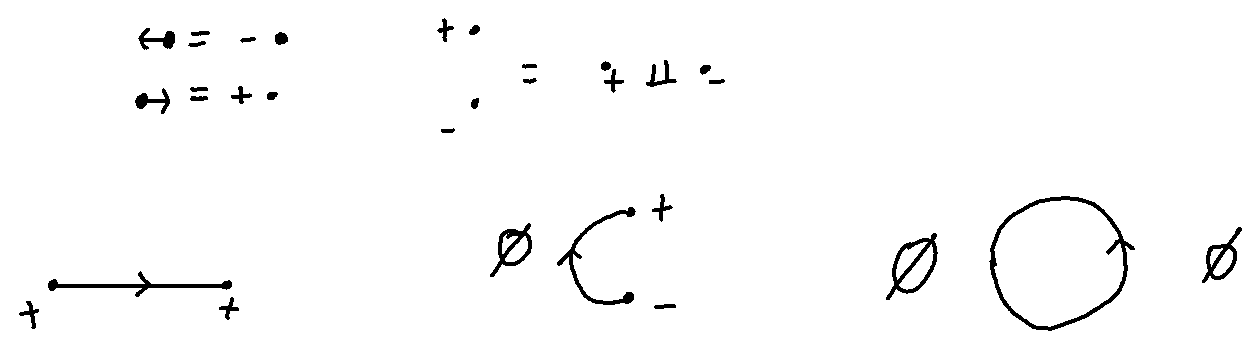
\includegraphics[width=9cm]{images/Lecture 11/1dBORDISM.png}\]
          
\end{ex}
\begin{ex}[Some objects and morphisms from $\Bord^{\operatorname{or}}_{2,1}$]

\[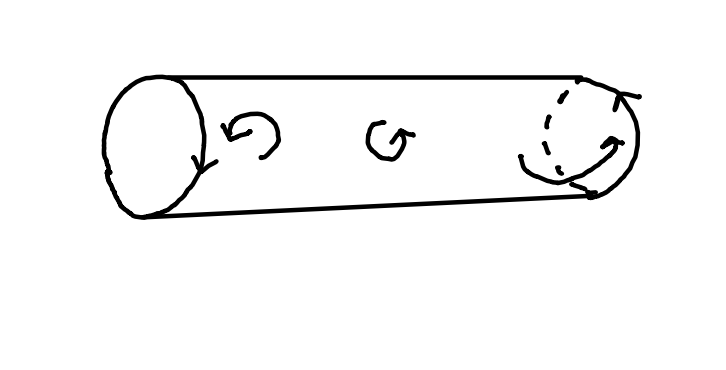
\includegraphics[width=6cm]{images/Lecture 11/2dBORDISM.png} \]
          

    Note that the orientation on the outgoing boundary is opposite to the induced orientation on the incoming one.
\end{ex}

We can also define analogous categories for other tangential structures, e.g. a framing.

\begin{ex}
    In 1 and 2 dimensions...
    %DRAWINGS
\end{ex}

\begin{defn}\label{DefDualObj}
    Let $\cat$ be a monoidal category. A left dual of an object $X \in \cat$ is an object $Y$ together with $ev_X: Y \otimes X \to \unit_\cat$ and $coev_X: \unit_\cat \to X \otimes Y$ such that
    
   % https://q.uiver.app/#q=WzAsMyxbMCwwLCJcXG1hdGhiYnsxfV9cXGNhdFxcb3RpbWVzIFhcXGNvbmcgWCJdLFsxLDEsIlhcXG90aW1lcyBZXFxvdGltZXMgWCJdLFsyLDAsIlhcXG90aW1lc1xcbWF0aGJiezF9X1xcY2F0XFxjb25nIFgiXSxbMCwxLCJjb2V2X1hcXG90aW1lcyBpaWRfWCIsMl0sWzEsMiwiaWRfWFxcb3RpbWVzIGV2X1giLDJdLFswLDIsImlkX1giLDAseyJvZmZzZXQiOi0xLCJzdHlsZSI6eyJoZWFkIjp7Im5hbWUiOiJub25lIn19fV0sWzAsMiwiIiwxLHsib2Zmc2V0IjoxLCJzdHlsZSI6eyJoZWFkIjp7Im5hbWUiOiJub25lIn19fV1d
	\begin{equation}
		\begin{tikzcd} \label{DUAL1}
			{\mathbb{1}_\cat\otimes X\cong X} && {X\otimes\mathbb{1}_\cat\cong X} \\
			& {X\otimes Y\otimes X}
			\arrow["{coev_X\otimes id_X}"', from=1-1, to=2-2]
			\arrow["{id_X\otimes ev_X}"', from=2-2, to=1-3]
			\arrow["{id_X}", from=1-1, to=1-3]
		\end{tikzcd}
	\end{equation}
	and
    
   % https://q.uiver.app/#q=WzAsMyxbMCwwLCJZXFxvdGltZXNcXG1hdGhiYnsxfV9cXGNhdFxcY29uZyBZIl0sWzEsMSwiWVxcb3RpbWVzIFhcXG90aW1lcyBZICJdLFsyLDAsIlxcbWF0aGJiezF9X1xcY2F0XFxvdGltZXMgWVxcY29uZyBZIl0sWzAsMSwiaWRfWVxcb3RpbWVzIGNvZXZfWSIsMl0sWzEsMiwiZXZfWVxcb3RpbWVzIGlkX1kiLDJdLFswLDIsImlkX1kiLDAseyJvZmZzZXQiOi0xLCJzdHlsZSI6eyJoZWFkIjp7Im5hbWUiOiJub25lIn19fV0sWzAsMiwiIiwxLHsib2Zmc2V0IjoxLCJzdHlsZSI6eyJoZWFkIjp7Im5hbWUiOiJub25lIn19fV1d
	\begin{equation}
   \label{DUAL2}
		\begin{tikzcd}
			{Y\otimes\mathbb{1}_\cat\cong Y} && {\mathbb{1}_\cat\otimes Y\cong Y} \\
			& {Y\otimes X\otimes Y }
			\arrow["{id_Y\otimes coev_Y}"', from=1-1, to=2-2]
			\arrow["{ev_Y\otimes id_Y}"', from=2-2, to=1-3]
			\arrow["{id_Y}", from=1-1, to=1-3]
		\end{tikzcd}
	\end{equation}
    The fact that these two diagrams commute is called snake relations. If the diagrams commute, then $X$ is the right dual of $Y$ and $Y$ is the left dual of $X$.
\end{defn}




\begin{rem}
    If $\cat$ is braided, and in particular for us symmetric, any right dual is a left dual and viceversa.
\end{rem}
\begin{notat}
    We denote the dual of an object $X$ with $X^\vee$. Sometimes it is also denoted with $X^\ast$.
\end{notat}
\begin{cor}\label{ImageOfDualStillDual}
    Let $F:\cat\to\dat$ be a monoidal functor. Thanks to monoidal functoriality, the monoidal unit $\unit_\cat$ is sent to $\unit_\dat$ (up to isomorphism), and hence one gets the evaluation map and coevaluation map: $ev_{F(X)}:F(Y)\otimes F(X)\to\unit_\dat\cong F(\unit_\cat)$ and $coev_{F(X)}:F(\unit_\cat)\cong\unit_\dat\to F(X)\otimes F(Y)$. Moreover, the image of a commuting diagram under a functor still commutes (see \ref{FunctorsPreserveCommut}). So, the dual objects are sent to dual objects by monoidal functors and $F(X^\vee)=F(X)^\vee$.
\end{cor}

\begin{ex}
\hfill
\begin{enumerate}
\item Any finite dimensional vector space $V$ has a dual, namely $V^\vee$:
    \begin{align}
        ev_V&: V^\vee \otimes V \to k\\
        coev_V &: k \to V \otimes V^\vee
    \end{align}
    %TODO write what is sent to what.
\item As an exercise try $\Set, \times$
\item $\cat = \Bordnor$.
The point $\bullet_+$ is dualizable with dual $\bullet_-$.
%DRAWING

This construction actually works for any object in $\Bordnor$ (and $\Bordn$).
\end{enumerate}
\end{ex}
\begin{defn}[Dual Morphisms]\label{DualMorph}
    Let $X,Y$ be dualizable objects in a symmetric monoidal category $\cat$ and $f:X\to Y$ be a morphism. The dual morphism is given by $$f^\vee:Y^\vee\xrightarrow{id_{Y^\vee} \otimes coev_X}Y^\vee\otimes X \otimes X^\vee\xrightarrow{id_Y^\vee\otimes f\otimes id_{X^\vee}}Y^\vee\otimes Y\otimes X^\vee\xrightarrow{ev_Y\otimes id_{X^\vee}}X^\vee$$
\end{defn}
\begin{defn}[Picard Groupoid]\label{PicardGroupoid}
    A Picard Groupoid is a symmetric monoidal category where every object is invertible with respect to $\otimes$ (i.e. $\forall A\in\cat\exists A^{-1}. A\otimes A^{-1}\cong\mathbb{1}_\cat$) and every morphism is an isomorphism, and hence it is a groupoid.
\end{defn}

\begin{lem}\label{BordDuals}
    In every bordism category $\Bord_{n,n-1}^{(\orient)}$ every object is dualizable.
\end{lem}
%DRAWING
\begin{lem}\label{DualizableMeansInvertibleNatTrans}
    Given symmetric monoidal categories $\cat$ and $\dat$, symmetric monoidal functors $F,G:\cat\to\dat$ and a symmetric monoidal natural transfromation $\alpha:F\Rightarrow G$, if $X\in\cat$ is dualizable, then $\alpha_X:F(X)\to G(X)$ is invertible.
\end{lem}
\begin{proof}
    We claim that the inverse is given by $\alpha_{(X^\vee)^\vee}$. Following \ref{DualMorph}, $\alpha_{(X^\vee)^\vee}:G(X^\vee)^\vee\to F(X^\vee)^\vee$. Note that $F(X^\vee)=F(X)^\vee$ and thus $F(X^\vee)^\vee=F(X)^{\vee\vee}=F(X)$ and so $\alpha_{(X^\vee)^\vee}:G(X)\to F(X)$. Remember that $ev_X:X^\vee\otimes X\to \unit_\cat$ and $coev_X:\unit_\cat\to X\otimes X^\vee$. We prove that the following diagram commutes
% https://q.uiver.app/#q=WzAsNixbMCwyLCJHKFgpXFxjb25nIEcoWClcXG90aW1lc1xcdW5pdF9cXGRhdCJdLFsxLDUsIkcoWClcXG90aW1lcyBHKFheXFx2ZWUpXFxvdGltZXMgRyhYKSJdLFsxLDAsIkcoWClcXG90aW1lcyBGKFheXFx2ZWUpXFxvdGltZXMgRihYKSJdLFsyLDEsIkcoWClcXG90aW1lcyBHKFheXFx2ZWUpXFxvdGltZXMgRihYKSJdLFsyLDUsIlxcdW5pdF9cXGRhdFxcb3RpbWVzIEcoWClcXGNvbmcgRyhYKSJdLFsyLDQsIlxcdW5pdF9cXGRhdFxcb3RpbWVzIEYoWClcXGNvbmcgRihYKSJdLFswLDEsImlkX3tHKFgpfVxcb3RpbWVzIEcoY29ldl9YKSIsMl0sWzAsMiwiaWRfe0coWCl9XFxvdGltZXMgRihjb2V2X1gpIl0sWzIsMSwiaWRfe0coWCl9XFxvdGltZXNcXGFscGhhX3tYXlxcdmVlfVxcb3RpbWVzXFxhbHBoYV9YIiwxXSxbMiwzLCJpZF97RyhYKX1cXG90aW1lc1xcZXRhX3tYXlxcdmVlfVxcb3RpbWVzIGlkX3tGKFgpfSJdLFsxLDQsIkcoZXZfe1h9KVxcb3RpbWVzIGlkX3tHKFgpfSIsMl0sWzMsNSwiRyhldl9YKVxcb3RpbWVzIGlkX3tGKFgpfSJdLFs1LDQsIlxcZXRhX3tYfSJdLFszLDEsImlkX3tHKFgpfVxcb3RpbWVzIGlkX3tHKFgpfVxcb3RpbWVzIFxcZXRhX1giLDFdXQ==
% https://q.uiver.app/#q=WzAsNixbMiwxLCJHKFgpXFxvdGltZXMgRihYXlxcdmVlKVxcb3RpbWVzIEYoWCkiXSxbMiwyLCJHKFgpXFxvdGltZXMgRyhYXlxcdmVlKVxcb3RpbWVzIEYoWCkiXSxbMSwwLCJHKFgpXFxjb25nIEcoWClcXG90aW1lc1xcdW5pdF9cXGRhdCJdLFsyLDQsIlxcdW5pdF9cXGRhdFxcb3RpbWVzIEYoWClcXGNvbmcgRihYKSJdLFswLDEsIkcoWClcXG90aW1lcyBHKFheXFx2ZWUpXFxvdGltZXMgRyhYKSJdLFswLDQsIlxcdW5pdF9cXGRhdFxcb3RpbWVzIEcoWClcXGNvbmcgRyhYKSJdLFsyLDQsIntpZF97RyhYKX1cXG90aW1lcyBHKGNvZXZfWCl9IiwyXSxbMiwwLCJ7aWRfe0coWCl9XFxvdGltZXMgRihjb2V2X1gpfSJdLFswLDQsIntpZF97RyhYKX1cXG90aW1lc1xcYWxwaGFfe1heXFx2ZWV9XFxvdGltZXNcXGFscGhhX1h9IiwxXSxbMCwxLCJ7aWRfe0coWCl9XFxvdGltZXNcXGFscGhhX3tYXlxcdmVlfVxcb3RpbWVzIGlkX3tGKFgpfX0iXSxbNCw1LCJ7Ryhldl97WH0pXFxvdGltZXMgaWRfe0coWCl9fSIsMl0sWzEsMywie0coZXZfWClcXG90aW1lcyBpZF97RihYKX19IiwxXSxbMyw1LCJ7XFxhbHBoYV97WH19Il0sWzEsNCwie2lkX3tHKFgpfVxcb3RpbWVzIGlkX3tHKFgpfVxcb3RpbWVzIFxcYWxwaGFfWH0iXV0=
\[\begin{tikzcd}
	& {G(X)\cong G(X)\otimes\unit_\dat} \\
	{G(X)\otimes G(X^\vee)\otimes G(X)} && {G(X)\otimes F(X^\vee)\otimes F(X)} \\
	&& {G(X)\otimes G(X^\vee)\otimes F(X)} \\
	\\
	{\unit_\dat\otimes G(X)\cong G(X)} && {\unit_\dat\otimes F(X)\cong F(X)}
	\arrow["{{id_{G(X)}\otimes G(coev_X)}}"', from=1-2, to=2-1]
	\arrow["{{id_{G(X)}\otimes F(coev_X)}}", from=1-2, to=2-3]
	\arrow["{{id_{G(X)}\otimes\alpha_{X^\vee}\otimes\alpha_X}}"{description}, from=2-3, to=2-1]
	\arrow["{{id_{G(X)}\otimes\alpha_{X^\vee}\otimes id_{F(X)}}}", from=2-3, to=3-3]
	\arrow["{{G(ev_{X})\otimes id_{G(X)}}}"', from=2-1, to=5-1]
	\arrow["{{G(ev_X)\otimes id_{F(X)}}}"{description}, from=3-3, to=5-3]
	\arrow["{{\alpha_{X}}}", from=5-3, to=5-1]
	\arrow["{{id_{G(X)}\otimes id_{G(X)}\otimes \alpha_X}}", from=3-3, to=2-1]
\end{tikzcd}\]
First of all, the triangle on the top commutes, i.e.
 $(id_{G(X)}\otimes\alpha_{X^\vee}\otimes\alpha_X)\circ(id_{G(X)}\otimes F(coev_X))=id_{G(X)}\otimes G(coev_X)$
 , because of the naturality of $\alpha$. The triangle underneath it also commutes, i.e.
  $id_{G(X)}\otimes\alpha_{X^{\vee}}\otimes\alpha_{X}=(id_{G(X)}\otimes id_{G(X)}\otimes\alpha_{X})\circ (id_{G(X)}\otimes\alpha_{X^{\vee}}\otimes id_{id_{F(X)}})$
    because of the unitality of $id_{G(X)}$ and $id_{F(X)}$.
    Lastly, the bottom trapezoid commutes thanks to the naturality of $\alpha$ and thus the whole big diagram commutes. 
    Consider now first mapping leftwards and successively downwards, i.e. $(G(ev_X)\otimes id_{G(X)})\circ id_{G(X)}\otimes G(coev_X)$, 
    this equals to the identity by one of the two snake relations of dual objects. 
    Take now the other route of the outer diagram, on the right;
     note that $(\alpha_X\vee)\vee=(G(ev_{X})\otimes id_{F(X)})\circ (id_{G(X)}\otimes\alpha_{X^\vee}\otimes id_{F(X)})\circ id_{G(X)}\otimes F(coev_{X})$ 
     by definition (\ref{DualMorph}) and hence the right route on the outer diagram corresponds to
      $\alpha_X\circ(\alpha_{X^\vee})^\vee$. Since the outer diagram commutes we obtain that
       $\alpha_X\circ(\alpha_{X^\vee})^\vee=id_{G(X)}$, i.e. $(\alpha_{X^\vee})^\vee$ is the right inverse of
        $\alpha_X$. One constructs a symmetric diagram by substituting $F$s with $G$s to prove that it is also the left inverse.
\end{proof}
\begin{cor}
    If every object in a symmetric monoidal category $\cat$ is dualizable, then any symmetric monoidal natural transformation between symmetric monoidal functors that have $\cat$ as the source category is invertible since a natural transfomation is invertible if and only if each of its components is invertible. Hence, $\Fun^\otimes(\cat,\dat)$ is a groupoid for any $\dat$ when all objects in $\cat$ are dualizable.
\end{cor}
\begin{cor}\label{TFTsareGRPDS}
    The category of topological field theories $\TFT_{n,n-1}^{or}(\cat)$ is a groupoid.
\end{cor}
\begin{lem}\label{InvDual}
    Any invertible object is dualizable.
\end{lem}
\begin{proof}
    Let $X$ be an invertible object. Then, there must be an $X^{-1}$ such that $X\otimes X^{-1}\cong\mathbb{1}_\cat$, the invertible object is the dual of $X$. The co/evaluation maps become isomorphisms the snake relations hold because if a commutative triangle of isomorphisms commutes in one direction, then it commutes also in the opposite one, i.e. for arbitrary isomorphisms $f,g,h$ such that $f=h\circ g$, it holds that $f^{-1}=(h\circ g)^{-1}=g^{-1}\circ h^{-1}$.
\end{proof}
\begin{lem}\label{InvertibleDualizable}
    A dualizable object is invertible if and only if its co/evaluation maps are isomorphisms.
\end{lem}
\begin{proof}
    $\implies$ directly follows from \ref{InvDual} since any invertible object has as co/evaluation maps isomorphisms. Conversely, suppose that $X$ is a dualizable object and the co/evaluation maps are isomorphisms. Then, there is a $Y\in\cat$ such that $ev_X:Y\otimes X\cong \mathbb{1}$.
\end{proof}
\begin{cor}
    If $\cat$ is a monoidal groupoid, then dualizable objects are invertible.
\end{cor}
\begin{proof}
    Since $\cat$ is a groupoid, then also the co/evaluation maps are isomorphisms. From \ref{InvertibleDualizable} it follows that the dualizable objects are invertible.
\end{proof}
\begin{cor}\label{PicardDualizable}
    A Picard groupoid (\ref{PicardGroupoid}) is equivalently a monoidal groupoid where every object is dualizable.
\end{cor}
\begin{ex}
    The underlying groupoid of $\Bordnor$ is a picard groupoid.
\end{ex}
\begin{notat}
We denote with $\cat^{\cong}$ the underlying groupoid of $\cat$, i.e. the subcategory of $\cat$ where we forget 
about non-invertible morphisms.
\end{notat}
\begin{notat}
We denote with $\cat^{\operatorname{fd}}$ (or sometiimes $\cat^{\operatorname{dualizable}}$) the subcategory of $\cat$ containing only dualizable objects.
We chose 'fd' because it can stand for two things:
\begin{itemize}
	\item 'finite dimensional' since dualizable objects in Vect are finite dimensional vector spaces and in general
	dualizability can be seen as a finiteness condition
	\item 'fully dualizable', a higher-categorical generalization of the notion of dualizability which we encounter
	 in the next subsection
\end{itemize}
\end{notat}
\subsection{Dualizability in higher categories \extra} % (fold)
\label{ssub:left_and_right_duals_in_higher_categories}
Equivalently, a left/right dual object $X$ in a monoidal category $\cat$ can also be
 characterized as a left/right adjoint
 when considered as a 1-morphism in the delooping (see
  \ref{DeloopingMonCat}) bicategory (see \ref{Bicategory}) $\mathbf{B}\cat$ of $\cat$.
  This
   makes sense because:
\begin{itemize}
    \item the evaluation map $ev_X$ corresponds to the counit $\epsilon$ of the adjunction 
    \item the coevaluation map $coev_X$ to the unit $\eta$ of the adjunction
    \item the two diagrams (\ref{DUAL1} and \ref{DUAL2}) to the triangle identities of the adjunction.
\end{itemize} 
A natural question is: what is an adjoint 1-morphism?
We defined only adjoint functors (see \ref{AdjFun})! 
Fortunately the definition we gave for functors, i.e.
1-morphisms in Cat, is easily generalizable to 1-morphisms in an arbitrary bicategory,
meaning that it is virtually the same: one just has to substitute '1-morphisms' for 'functors'
and substitute '2-morphisms' for 'natural
transformations' (when talking about the co/evaluation and the identity on the functors).

A sane individual, i.e. not a homo categoriens\footnote{A subspecies of homo sapiens.
	 Exemplars usually say stuff like 
	 '\href{https://ncatlab.org/nlab/show/differential+equation}{I understand differential equations as sub-$\infty$-groupoids of tangent and jet bundles}'
	  and have posters of Grothendieck or Lawvere in their bedroom.}
, might ask why this is remotely useful. The answer is that one needs this intuition to talk about
 monoidal ($\infty,n$)-categories with duals. This is interesting for us because, for 
 instance,  these objects are used in the cobordism hypothesis, stating that their objects
  classify fully extended TFTs,
  see \ref{RemarkOnCobHypo}.
\begin{rem}
    The notion of delooping of a monoidal category as a one-object bicategory can be
     generalized to monoidal $(\infty,n)$-categories. The delooping of a monoidal
      $(\infty,n)$-category $\cat$ is a one-object $(\infty,n+1)$-category $\mathbf{B}\cat$ where the objects of $\cat$ are the 1-morphisms of $\mathbf{B}\cat$ and the tensor product of $\cat$ is the composition $\circ$ of 1-morphisms.
\end{rem}
\begin{defn}[($\infty,n$)-monoidal categories with duals]\label{HigherMonCatDuals}
    Let $\cat$ be a monoidal ($\infty,n$)-category. Then $\cat$ has duals if and only if its delooping $\mathbf{B}\cat$ has adjoints\footnote{In the usual jargon, an $(\infty,n)$-category has adjoints if it has adjoints
    	 for any $k$-morphism with $0<k<n$. We spelled what it means anyway for the sake of clarity.} for any $k$-morphism with $0<k<n+1$ . We say that any object in such a
    	  category is fully $n$-dualizable. 
\end{defn}
We have a vague idea of what are monoidal ($\infty,n$)-categories and deloopings
thereof. However, we did not sketch what it means that an ($\infty,n+1$)-category has
 adjoints, but it is essential to understand this definition
  since we characterized the duals of a monoidal
  ($\infty,n$)-category in terms of the adjoints of its delooping.
  The idea is to trace this back to adjoints of 1-morphisms in bicategories.
  \begin{defn}[Homotopy 2-category of an $(\infty,n)$-category]
A homotopy 2-category of an $(\infty,n)$-category $\cat$ with $n\geq 2$ is a bicategory h$_{2}\cat$
with 
\begin{itemize}
\item  the objects of $\cat$ as objects $$\operatorname{ob}(\cat)=\operatorname{ob}(\operatorname{h}_2\cat)$$
\item the 1-morphisms of $\cat$ as 1-morphisms 
$$1\operatorname{-mor}(\cat)=1\operatorname{-mor}(\operatorname{h}_2\cat)$$ 
\item isomorphism classes of 2-morphisms in $\cat$ as 2-morphisms, i.e. given
1-morphisms $f,g:X\to Y$ a 2-morphism in $\operatorname{h}_2\cat$ is a 2-morphism in $\cat$
up to 3-isomorphism
 $$2\operatorname{-mor}(\cat)/_{\cong}=2\operatorname{-mor}(\operatorname{h}_2\cat)$$ 
\end{itemize}
  \end{defn}
  \begin{defn}[Adjoints in $(\infty,n)$-categories]
We define adjoints for $k$-morphisms by recursion.
An $(\infty,n)$-category $\cat$ has adjoints for 1-morphisms if its homotopy 2-category 
$\operatorname{h}_2\cat$ has adjoints for 1-morphisms, i.e. if all 1-morphisms of
 $\operatorname{h}_2\cat$ are part of an adjunction. An $(\infty,n)$-category $\cat$ has
  adjoints for $k$-morphisms if, for every pair $X,Y\in\operatorname{ob}(\cat)$, the 
  $(\infty,n-1)$-category $\Hom_{\cat}(X,Y)$ has adjoints for $k-1$-morphisms.
  \end{defn}
  We say that an $(\infty,n)$-category has adjoints if it has adjoints for any $k$-morphism 
  with $0<k<n$. 
  
  Having defined adjoints of morphisms of an $(\infty,n)$-category, we now have all the
  necessary pieces of the puzzle constituiting the sketch
   of what it means that a monoidal $(\infty,n)$-category
  has duals.
\begin{rem}
There is an equivalent definition of monoidal $(\infty,n)$-category with duals, see \cite{lurie2009classification} and
\cite{gwilliam2018duals}. This intuition about adjoints is very useful also in this case.
\end{rem}

% -------------------------------------------------------------
% --------------------- LECTURE 12 4-6/12 ---------------------
% -------------------------------------------------------------
% flipped classroom

\chapter{Classification of topological field theories}\label{ClassificationOfTFTs}
\epigraph{
\textbf{Existence}: Why is there something, rather than nothing?

\noindent This does not seem very accessible by current methods. A more realistic
goal may be

\noindent \textbf{Classification}: Given that there’s something, what could it be?}{Jack Morava in \cite{morava2011cosmic}}
%Sorry if too quirky XD feel free to delete it of course, was also undecided if to put it here or for classification of 2d manifolds /Andrea

In this chapter, we classify 1d-TFTs and 2d-TFTs, provide a sketch on how that might work for 3d-TFTs 
and show surprsising connections between knot theory and 3d-TFTs.

Roughly, our classifications theorems will be equivalence of categories of this kind 
$$ev_{X\in\Bord_{n}}:\Fun^{\otimes}(\Bord_{n},\cat)\simeq(\cat^{\operatorname{fd}})^{\cong}$$
meaning that evaluating a TFT on an object of $\Bord_{n}$ induces an equivalence of categories. 
To be clear, recall that: 
\begin{itemize}
\item $\Bord_n$ is the category of $n$-bordisms
\item $\Fun^{\otimes}(\Bord_{n},\cat)$ is the category of $n$-dimensional topological field theories since they are symmetric monoidal functors from the category of $n$-bordisms to some symmetric monoidal category
\item $(\cat^{\operatorname{fd}})^{\cong}$ is the Picard groupoid underlying $\cat$ since
 $\cat^{\operatorname{fd}}$ is the subcategory of $\cat$ contatining only dualizable
 objects and $(\cat^{\operatorname{fd}})^{\cong}$ is the maximal underlying groupoid, restricting dualizable objects in
  $\cat^{\operatorname{fd}}$ to invertible ones
\end{itemize}

A natural question
is: how is this a \emph{classification}? This sort of statement certainly looks different 
from other classifications, for example the one of 2-dimensional manifolds we have seen in this course
 (\ref{Classification of 2 manifolds}). Such an equivalence of categories classifies TFTs because every $n$-TFT is
  determined by where it sends an object in $\Bord_{n}$ and thus TFTs are classified by where they send
   such $n-1$-manifold, without specifying how the functor acts on morphism, i.e. the bordisms. Moreover,
   given a dualizable object of $\cat$ one can construct a TFT since the equivalence goes also 
   in the other direction, so one can say that TFTs are classified by the dualizable objects (up to isomorphism)
    of their target category.
   
   Sketchily, our strategy to prove these results will be to find generators and relations for $\Bord_{n}$ and then
    check where they are sent to. It will follow that dualizable objects in $\cat$ already provide all the information
    we need to know to determine what is the TFT in question: where the generators and relations of $\Bord_{n}$
    are sent to.
    \section{Classification of 1d-TFTs}\label{ClassificationOf1dTFTs}
The main goal of this subsection is to prove that given an oriented 1d-TFT
 $\Zf:\Bord_{1,0}\to\cat$, $\Zf(\bullet)$ has a dual and conversely, given an object $X\in\cat$
  in the target category of the TFT we can reconstruct a 1d-TFT.
\begin{thm}[Classification of 1-dimensional bordisms]\label{class1dBord}
Any connected oriented 1-dimensional manifold with boundaries is diffeomorphic to one of 
the following manifolds: 

\[\includegraphics[width=8cm]{images/Lecture 12/All1Bordisms.png} \]
	


\end{thm}
For the proof we refer to the appendix of \cite{Milnor1997topology}.

This means that any 1-dimensional bordism (i.e. including disconnected ones)
 is diffeomorphic to a disjoint union of such bordisms. Since in $\Bord_{1,0}$ bordisms are taken up to orientation
 preserving diffeomorphisms, this means that in $\Bord_{1,0}$ all morphisms \emph{are} tensor products of 
 the listed manifolds.
  Moreover, we know that the objects of $\Bord_{1,0}$ are just disjoint unions of $\bullet_{+}$ and $\bullet_-$.
 Hence, we now know the generators of $\Bord_{1,0}$, i.e. $\bullet_{+}$ and $\bullet_-$, and the relations, 
 i.e. the possible connected 1-dimensional bordisms. Since we also know that $\Zf$ is a 
 \emph{symmetric monoidal} functor, it means that we shall just check where such generators and relations are sent,
 see \ref{AlternativeProof1d}.
 

\begin{rem}
    By $(\cat^{{\operatorname{fd}}})^{\cong}$ we denote the restriction of a symmetric monoidal category on its dualizable objects and its isomorphisms, said briefly: a restriction on the underlying Picard groupoid because in any symmetric monoidal groupoid an object is dualizable if and only if it is invertible (see \ref{PicardDualizable}).
\end{rem}
\begin{thm}\label{thm:classif_of_1dtft}
    Let $\cat$ be a symmetric monoidal category. Then the map\footnote{There is unfortunately a notational clash between what we called the evaluation map for dualizable objects, denoted by $ev$, and what we also call in this case evaluation map, denoted by $\mathcal{E} V$. In the latter case, we are referring to a similar convention we use for example in topology when we call a map of this genre $Map(\ast,X)\to X$ an evaluation map. The intuition is that we feed an element of the domain into a map, a functor in our case, and see what happens, "evaluate it".} 
    \begin{align}
    	\TFT_{1,0}^{or}=\Fun^{\otimes}(\Bord_{1,0}^{or},\cat)&\xrightarrow{\mathcal{E} v_{\bullet_{+}}}(\cat^{\operatorname{fd}})^{\cong} \\
    	\Zf&\mapsto \Zf(\bullet_+)
    \end{align}
    is a symmetric monoidal equivalence of groupoids. 
    % https://q.uiver.app/#q=WzAsNCxbMCwwLCJURlRfezEsMH1ee29yfSJdLFswLDIsIihcXGNhdF57ZHVhbGl6YWJsZX0pXntcXGNvbmd9Il0sWzEsMSwiXFxjYXRee2R1YWxpemFibGV9Il0sWzIsMCwiXFxjYXQiXSxbMCwxXSxbMSwyLCJpIiwyLHsic3R5bGUiOnsidGFpbCI6eyJuYW1lIjoiaG9vayIsInNpZGUiOiJ0b3AifX19XSxbMCwyLCIiLDEseyJzdHlsZSI6eyJib2R5Ijp7Im5hbWUiOiJkYXNoZWQifX19XSxbMCwzLCJcXG1hdGhjYWx7RX1WIl0sWzIsMywiaiIsMix7InN0eWxlIjp7InRhaWwiOnsibmFtZSI6Imhvb2siLCJzaWRlIjoidG9wIn19fV1d
\[\begin{tikzcd}
	{\TFT_{1,0}^{or}} && \cat \\
	& {\cat^{\operatorname{fd}}} \\
	{(\cat^{\operatorname{fd}})^{\cong}}
	\arrow["{\simeq}", from=1-1, to=3-1]
	\arrow["i"', hook, from=3-1, to=2-2]
	\arrow[dashed, from=1-1, to=2-2]
	\arrow["{\mathcal{E}v_{\bullet_{+}}}", from=1-1, to=1-3]
	\arrow["j"', hook, from=2-2, to=1-3]
\end{tikzcd}\]
\end{thm}
\noindent The image of $\mathcal{E}v_{\bullet_{+}}$ is in $(\cat^{\operatorname{fd}})^{\cong}$, since 
\begin{enumerate}
    \item $\TFT_{1,0}^{\orient}$ is a groupoid, and functors preserve isomorphisms
    \item Every object in $\Bord_{1,0}^{\orient}$ is dualizable and, because of functoriality, the image of a dualizable object remains a dualizable object.
\end{enumerate}
%Note that there's nothing special about dimension 1 here. We then have such an evaluation functor into $(\cat^{\operatorname{fd}})^{\cong}$ in every dimension, i.e. from all $\TFT_{1,0}^{or}$. Dimension 1 is then special because this map is actually an equivalence. %%% Can't understand what is meant here /Andrea
\begin{proof}
	The following proof is the closest to what we did in class and is from \cite[Theorem 16.10]{FreedBordism}.
	
    We need to prove three things to demonstrate that $\mathcal{E}V_{\bullet_{+}}$ is an equivalence: that it is full, faithful and essentially surjective:
    \begin{enumerate}
        \item Trivially, note that since $\mathcal{E}V_{\bullet_{+}}$ lands in $(\cat^{\operatorname{fd}})^{\cong}$
        then it must be essentially surjective since any two objects are isomorphic.
        \item It is faithful: let $\Zf,\Zf'\in \TFT_{1,0}^{or}$ and $\alpha,\beta:\Zf\Rightarrow\Zf'$ be natural
         transformations between them and hence isomorphisms (see \ref{TFTsareGRPDS}). Suppose that
          $\mathcal{E}V_{\bullet_{+}}(\alpha)=\mathcal{E}V(\beta)$, i.e. $\alpha^{1}_{\bullet_+}=\alpha^{2}_{\bullet_+}$ since $\mathcal{E}V_{\bullet_{+}}$ evaluates on the point.
        Recall that $\bullet_-=\bullet_+^\vee$. We have that for any natural isomorphism
         $\eta$ it holds that $\eta{\bullet_+^\vee}=(\eta{\bullet_+})^\vee$ because of functoriality and
          $\eta_{\bullet_-}=(\eta{\bullet_+}^\vee)^{-1}$ 
          because of \ref{DualizableMeansInvertibleNatTrans}. 
          From this it follows that
           $\alpha_{\bullet_-}=(\alpha_{\bullet_+}^\vee)^{-1}=(\beta{\bullet_+}^\vee)^{-1}=\beta_{\bullet_-}$. 
           With a specular proof we can prove that $\alpha_{\bullet_+}=\beta_{\bullet_+}$. 
           Since 0-dimensional compact manifolds are just finite disjoint unions of $\bullet_+$ or $\bullet_-$ and
            $\alpha$ and $\beta$ are symmetric monoidal natural transformations
           it follows that for any $X\in\Bord_{1,0}^{or}$, $\alpha_X=\beta_X$. 
           This proves that $\mathcal{E}V$ is faithful because it implies that for any two natural transformations that
            are mapped to equal morphisms in $\cat$ must be also equal in $\Fun^{\otimes}(\Bord_{1,0},\cat)$
        \item $\mathcal{E}V_{\bullet_{+}}$ is full. Given an arbitrary isomorphism $f:X\to X'$
         in $(\cat^{\operatorname{fd}})^{\cong}$ we now show that there is an isomorphism $\eta:\Zf\Rightarrow\Zf'$
         in $\Fun^{\otimes}(\Bord_{1,0},\cat)$ such that $\mathcal{E}V_{\bullet_{+}}(\eta)=\eta_{\bullet_{+}}=f$.
         So, we define $f=\eta$ and thus $(f^{\vee})^{-1}$.
          Objects in
          $(\cat^{\operatorname{fd}})^{\cong}$ are sequences of tensor products of $X$ and $X^\vee$. Hence,
          using the trick we used before we can extend any natural transformation $\eta:\bullet_{+}\to\bullet_{+}$
         to a disjoint union of such natural transfomations, via the monoidal structure on $\Bord_{1,0}$, since 
         any object $X\in\Bord_{1,0}$ is diffeomorphic to a finite disjoint union of $\bullet_{+}$ and $\bullet_-$, 
         and we know that
          $(\alpha_{\bullet_{+}}^{\vee})^{-1}$. This is  independent of the choice of the
           diffeomorphism between 
         $X$ and disjoint unions of $\bullet_{+}$ and $\bullet_-$ thanks to the coherence of the chosen map $\eta_{X}$.
         %I do not understand what th coherence of \eta_Y should be, naturality? Something to do with the monoidal structure? why does Freed switch continuously between X and Y for the object we are considering argh!!
         Moreover, the diffeomorphism is determined up to permutation also because of the coherence of $\eta_X$
         . It remains to show that $\eta_X$ is an isomorphism. $\eta_X$ can be a disjoint union of the 5 1-bordisms
         (\ref{class1dBord}) and hence, thanks to symmetric monoidality of $\eta$, we can just check these 5.
         The two identities are trivially isomorphisms.
         Then we need to check that the following diagram commutes to check for the coevaluation 
         % https://q.uiver.app/#q=WzAsMyxbMCwwLCJcXFpmKFxcYnVsbGV0Xy0pXFxvdGltZXNcXFpmKFxcYnVsbGV0XyspIl0sWzIsMCwiXFxaZicoXFxidWxsZXRfLSlcXG90aW1lc1xcWmYnKFxcYnVsbGV0XyspIl0sWzEsMSwiXFx1bml0X1xcY2F0Il0sWzAsMSwiZlxcY2lyYyAoZl57XFx2ZWV9KV57LTF9Il0sWzIsMCwiXFxaZihjb2V2X1gpIl0sWzIsMSwiXFxaZicoY29ldl9YKSIsMl1d
         \[\begin{tikzcd}[cramped]
         	{\Zf(\bullet_-)\otimes\Zf(\bullet_+)} && {\Zf'(\bullet_-)\otimes\Zf'(\bullet_+)} \\
         	& {\unit_\cat}
         	\arrow["{f\circ (f^{\vee})^{-1}}", from=1-1, to=1-3]
         	\arrow["{\Zf(coev_X)}", from=2-2, to=1-1]
         	\arrow["{\Zf'(coev_X)}"', from=2-2, to=1-3]
         \end{tikzcd}\]
         %aren't we just checking if the coevaluation makes sense now? But before Freed said we want to check if they are isomorphisms arghhh! 
         
          %very confused by Freed's proof, I just shut off my brain and copied it, I could not else, please check A/andrea  
          The commutativity of this diagram follows from the fact that the following diagram commutes
        % https://q.uiver.app/#q=WzAsNixbMCwwLCJcXHVuaXRfXFxjYXQiXSxbMCwyLCJcXFpmJyhcXGJ1bGxldF8tKVxcb3RpbWVzXFxaZicoXFxidWxsZXRfKykiXSxbMCw0LCJcXFpmKFxcYnVsbGV0Xy0pXFxvdGltZXNcXFpmKFxcYnVsbGV0XyspXFxvdGltZXMgXFxaZicoXFxidWxsZXRfLSlcXG90aW1lc1xcWmYnKFxcYnVsbGV0XyspIl0sWzIsMCwiXFxaZihcXGJ1bGxldF8tKVxcb3RpbWVzXFxaZihcXGJ1bGxldF8rKSJdLFsyLDIsIlxcWmYoXFxidWxsZXRfLSlcXG90aW1lc1xcWmYnKFxcYnVsbGV0XyspIl0sWzIsNCwiXFxaZihcXGJ1bGxldF8tKVxcb3RpbWVzXFxaZicoXFxidWxsZXRfKylcXG90aW1lcyBcXFpmJyhcXGJ1bGxldF8tKVxcb3RpbWVzXFxaZicoXFxidWxsZXRfKykiXSxbMCwxLCJcXFpmJyhjb2V2X1gpIiwyXSxbMSwyLCJcXFpmKGNvZXZfeClcXG90aW1lcyBpZF97XFxaZicoXFxidWxsZXRfLSl9XFxvdGltZXMgaWRfe1xcWmYnKFxcYnVsbGV0XyspfSIsMV0sWzAsMywiXFxaZihjb2V2X1gpIl0sWzMsMiwiaWRfe1xcWmYoXFxidWxsZXRfLSl9XFxvdGltZXMgaWRfe1xcWmYoXFxidWxsZXRfKyl9XFxvdGltZXMgXFxaZihjb2V2X3gpIiwxXSxbMyw0LCJpZF97XFxaZihcXGJ1bGxldF97LX0pfVxcb3RpbWVzIGYiXSxbMiw1LCJpZF97XFxaZihcXGJ1bGxldF8tKX1cXG90aW1lcyBmXFxvdGltZXMgaWRfe1xcWmYnKFxcYnVsbGV0Xy0pfVxcb3RpbWVzIGlkX3tcXFpmJyhcXGJ1bGxldF8rKX0iLDJdLFs0LDUsImlkX3tcXFpmKFxcYnVsbGV0Xy0pfVxcb3RpbWVzXFxaZicoY29ldl94KVxcb3RpbWVzIGlkX3tcXFpmKFxcYnVsbGV0XyspfSIsMV1d
        \[\begin{tikzcd}[cramped]
        	{\unit_\cat} && {\Zf(\bullet_-)\otimes\Zf(\bullet_+)} \\
        	\\
        	{\Zf'(\bullet_-)\otimes\Zf'(\bullet_+)} && {\Zf(\bullet_-)\otimes\Zf'(\bullet_+)} \\
        	\\
        	{\Zf(\bullet_-)\otimes\Zf(\bullet_+)\otimes \Zf'(\bullet_-)\otimes\Zf'(\bullet_+)} && {\Zf(\bullet_-)\otimes\Zf'(\bullet_+)\otimes \Zf'(\bullet_-)\otimes\Zf'(\bullet_+)}
        	\arrow["{\Zf'(coev_X)}"', from=1-1, to=3-1]
        	\arrow["{\Zf(coev_x)\otimes id_{\Zf'(\bullet_-)}\otimes id_{\Zf'(\bullet_+)}}"{description}, from=3-1, to=5-1]
        	\arrow["{\Zf(coev_X)}", from=1-1, to=1-3]
        	\arrow["{id_{\Zf(\bullet_-)}\otimes id_{\Zf(\bullet_+)}\otimes \Zf(coev_x)}"{description}, from=1-3, to=5-1]
        	\arrow["{id_{\Zf(\bullet_{-})}\otimes f}", from=1-3, to=3-3]
        	\arrow["{id_{\Zf(\bullet_-)}\otimes f\otimes id_{\Zf'(\bullet_-)}\otimes id_{\Zf'(\bullet_+)}}"', from=5-1, to=5-3]
        	\arrow["{id_{\Zf(\bullet_-)}\otimes\Zf'(coev_x)\otimes id_{\Zf(\bullet_+)}}"{description}, from=3-3, to=5-3]
        \end{tikzcd}\]
    \end{enumerate}
    The argument for the evaluation of $X$ is specular. From there also the map for the circle follows since 
    the circle is just a composition of evaluation and a coevaluation with a braiding in between. Note that
    the commutativity of the circle means that $\Zf(S^1)=\Zf'(S^1)$.
\end{proof}
\begin{rem}
	The author of this part of the notes was very confused for a long time 
	by the proof just provided. They cannot understand 
	Freed's line of argument when it comes to the proof of the fullness of $\mathcal{E}V_{\bullet_{+}}$, probably 
	because of	notational choices and some typos. Hence, we now give 2 alternative proofs, in order to make it 
	as clear as possible.
\end{rem}
%modified a bit from the lecture, but I am confident it makes sense /andrea
\begin{thm}[Alternative formulation of the classification of 1TFTs]
	Let $X\in\cat$ be a dualizable object. Specifying $\Zf(\bullet_{+})=X$ determines a 1d-TFT.
\end{thm}
%\begin{proof}[Proof of the classification of 1-TFTs 2.0]
	
%	Set $\Zf( \bullet_{+})=X$ where $X\in\cat^{\operatorname{fd}}$ and $\Zf(\bullet_{-})=Y$ 
	 %since we need to respect the symmetric monoidality of $\Zf$ and symmetric monoidal functors must send
	%dual objects in the source category to dual objects in the target category.
	%	$$\Zf(\bullet_+):=X$$ 
%	$$\Zf(\bullet_-):=Y$$
%	$$\Zf(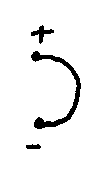
\includegraphics[scale=0.17]{images/Classification 1TFT/evaluation.png}):=ev_X$$
%	$$\Zf(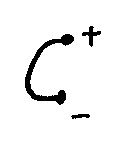
\includegraphics[scale=0.17]{images/Classification 1TFT/coevaluation.png}):=coev_X$$
%	An arbitrary compact 0-dimensional manifold
%	$M\in\Bord_{1,0}$
%	is a finite disjoint union of $\bullet_+,\bullet_-$. Thus, by a diffemorphism permuting the points 
%	$$M\cong(\amalg_{I}\bullet_+)\amalg(\amalg_{J}\bullet_-)$$
%	where $I,J\subseteq\N$. For any $M\in\Bord_{1,0}$, $\Zf$ to behave as follows, i.e. is symmetric monoidal
%%	$$\Zf(M):=(\bigotimes_{I}X)\otimes(\bigotimes_{J}Y)$$
%	By coherence of the symmetric monoidal structure, especially how the braiding and the associatior 
%%	Thanks to \ref{class1dBord}, we know that any oriented 1-dimensional bordism is diffeomorphic to a disjoint union
%	of the manifolds in \ref{class1dBord}. Since $\Zf$ is symmetric monoidal, it is sufficient to determine
%\end{proof}

\begin{proof}[Proof of the classification of 1-TFTs 2.0]\label{GeneratorsClass1TFT}
An alternative proof relies proves the equivalence in the other direction and relies on the fact that since the functor
 is \emph{symmetric} monoidal one can just check what the TFT does only for 5 of all the possible 
 connected 1-dimensional bordisms (\ref{class1dBord}), not considering what happens for the other 3 ones with the
  reversed orientations without loss of generality because $\Bord_{1,0}$ is symmetric monoidal.
   We took it from \cite[Example 1.1.9]{lurie2009classification}
  
  First we need to determine where $\bullet_+,\bullet_-\in\Bord_{1,0}$ are sent. Since they are duals of one another,
  they are dualizable objects and thus they are sent to $X,X^{\vee}\in\cat^{\operatorname{fd}}$,
   e.g. finite dimensional vector spaces in the case of $\Vect_{k}$. An arbitrary objects of $M\in\Bord_{1,0}$
   is a finite disjoint union of $\bullet_+,\bullet_-$, i.e. 
   $$M=(\amalg_{I}\bullet_+)\amalg(\amalg_{J}\bullet_-)$$
    where $I,J\subseteq\N$. Thanks to the symmetric monoidal functoriality of $\Zf$ we have that 
    $$\Zf(M)=(\bigotimes_{I}X)\otimes(\bigotimes_{J}X^\vee)$$
     Now we need to understand where the 5 possible 1-bordisms are sent.
  \begin{enumerate}
  	\item $\Zf(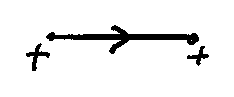
\includegraphics[scale=0.18]{images/Classification 1TFT/identityplus.png})=id_{X}$
  	\item$\Zf(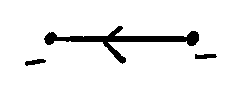
\includegraphics[scale=0.18]{images/Classification 1TFT/identityminus.png})=id_{X^\vee}$
  	\item $\Zf(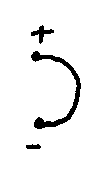
\includegraphics[scale=0.17]{images/Classification 1TFT/evaluation.png})=ev_{X}$, hence $X\amalg X^\vee\xrightarrow{ev_{X}} \unit_{\cat}$ and more precisely for $v\in X\in\Vect_{k}$: $ev_{X}:(X,\lambda)\mapsto \lambda(v)$
  	\item $\Zf(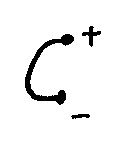
\includegraphics[scale=0.15]{images/Classification 1TFT/coevaluation.png})=coev_{X}$, hence $\unit_{\cat}\xrightarrow{coev_{X}}X\otimes X^\vee$ and more precisely for $\lambda\in k\in\Vect_{k}$, via the canonical isomorphism $X\otimes X^\vee\cong\operatorname{End}(X)$, $coev_X$ corresponds to taking the trace
  	\item $\Zf(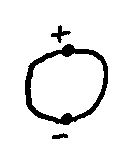
\includegraphics[scale=0.15]{images/Classification 1TFT/circle.png})=coev_X \circ ev_{X}$, hence $\unit_{\cat}\xrightarrow{coev_X \circ ev_{X}}\unit_{\cat}$, and, following the cases for $\Vect_{k}$ treated in the previous two points, to taking the trace of the identity matrix, i.e. the dimension of $X$
  \end{enumerate}
  
  The moral of the story is that a TFT is uniquely
  determined, up to isomorphism, once one knows $X\in\cat^{\operatorname{fd}}$ since then one knows 
  \begin{itemize}
  	\item what $X^\vee$ is, what finite sequences of tensored $X$ and $X^\vee$ are, which will
  	 be sent to finite
  	 disjoint unions of $\bullet_{+}$ and $\bullet_-$ (aka all the objects of $\Bord_{1,0}$);
  	 \item what $id_X$ and $id_{X^\vee}$ are
  	 \item what $ev_X$ and $coev_X$ are and hence also $coev_X\circ ev_X$
  \end{itemize}
  
\end{proof}
\begin{rem}
Lurie considers 5 possible
bordisms and not all 8, thereby excluding some possible orientations. However, Lurie's
 argument is without loss of
generality because it implicitly relies 
on the \emph{symmetric} monoidality of $\Bord_{1,0}$ since, for instance, one can get
 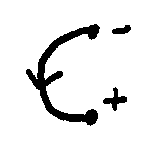
\includegraphics[width=0.7cm]{images/Lecture 12/coevminusplus.png}  by composing
  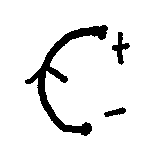
\includegraphics[width=0.7cm]{images/Lecture 12/coevplusminus.png} with a
braiding. 

Anyways, we hold that there is a clearer way to demonstrate this result in a similar vein, which
 relies on the following
 result.
\end{rem}
\begin{lem}
All 1-dimensional bordisms are generated by the generators: 
\[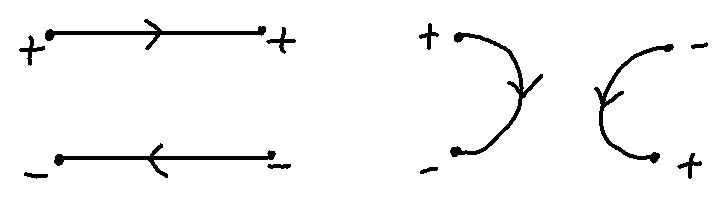
\includegraphics[width=7cm]{images/Lecture 12/generators.png} \]

and the relation 

\[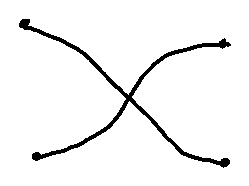
\includegraphics[width=3cm]{images/Lecture 12/relations.png} \]	
		\end{lem}
\begin{proof}
We need to show that there is a way of gluing our generators and the braiding relation to get the other 4 manifolds of \ref{class1dBord}.

\begin{enumerate}
\item 	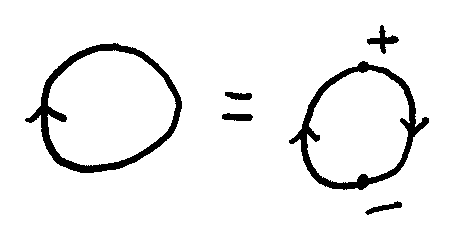
\includegraphics[width=3cm]{images/Lecture 12/circle1.png} 
\item 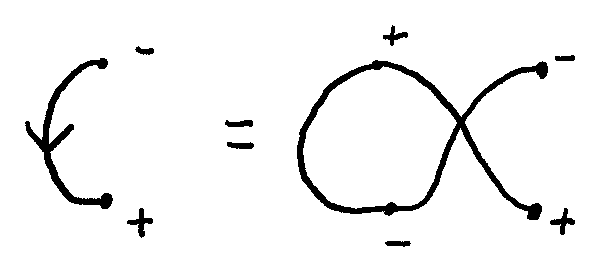
\includegraphics[width=3cm]{images/Lecture 12/coevaluationbraiding.png} 
\item  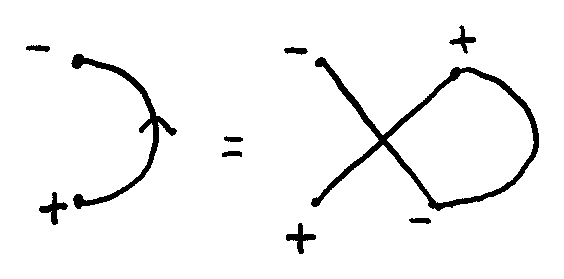
\includegraphics[width=3cm]{images/Lecture 12/evaluationbraiding.png} 
\item 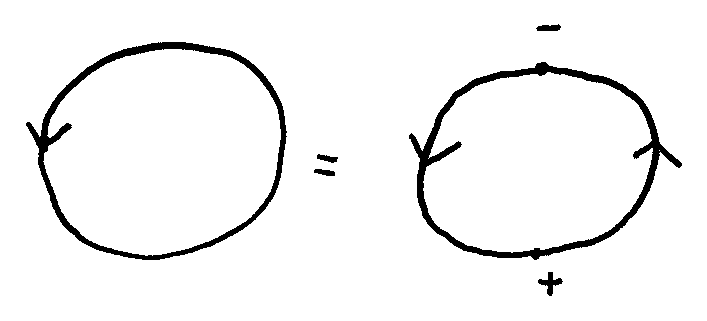
\includegraphics[width=3cm]{images/Lecture 12/circle2.png} 
\end{enumerate}
\end{proof}

\begin{proof}[Proof of the classification of 1-TFTs 2.1 ]
 In this proof we rely on the lemma we just proved. We need to show where the objects, the
  generators and the relation
  are sent to. Fortunately, we showed already in the proof took from Lurie's paper
   (\ref{GeneratorsClass1TFT}) where
   the objects and our generators are sent to. It remains to show where the braiding relation
    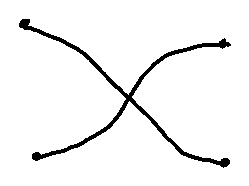
\includegraphics[width=0.54cm]{images/Lecture 12/relations.png} is sent to.
    Since $\Zf$ is a symmetric monoidal functor, the braiding in $\Bord_{1,0}$ is sent to the
     braiding in the target
     category $\cat$.
 \end{proof}

The classification of 1-dimensional topological field theories is the simplest case of an
 important guiding hypothesis
 in the field of TFTs, the cobordism hypothesis, see \ref{RemarkOnCobHypo}. It is the only
  case in which so-called
 extended TFTs coincide with non-extended ones, i.e. the usual Atiyah-Segal definition as a
  simple symmetric 
 monoidal functor we are using.

Recap: $\TFT_{1,0}^{or}(\cat) \xrightarrow{\mathscr Ev_{\bullet+}} (\cat^{\fd})^{\simeq} \hookrightarrow \cat$. The map is the following: $\Zf \mapsto \Zf(\bullet_+)$.

Now we classified 1 dimensional TFTs, we would now like to do the same for 2 dimensional TFTs.
We will find out that there is an equivalence between $\TFT_{2,1}^{or}(\cat)$ and commutative Frobenius algebras.

\section{Classification of 2d-TFTs}
As we have done for the 1-dimensional case, we now try to classify 2-dimensional TFTs. For a more detailed proof see Kock \cite{kock_2003} or the lecture notes from Schweigert \cite{SchwHopfQuantumTFT}. 

We have already defined the following notions in arbitrary monoidal categories (see \ref{FrobAlg}, \ref{MonObj}, \ref{ComonObj}, \ref{CommFrobAlg}, \ref{CommBim}). However, we now explicitly state how the abstract formal definitions are instantiated in Vect$_k$.
\begin{defn}[Algebra over a Field]
    An algebra\footnote{Note that for us algebras are \textbf{always} associative and unital.} over a field $k$ is a monoid object (\ref{MonObj}) in $\Vect_k$. More generally a left/right $R-$algebra is a monoid object in the category of left/right $R-$modules. The latter generalization holds also for the next definitions of $k-$coalgebra, $k-$bialgebra and Frobenius $k-$algebra.
\end{defn}
\begin{defn}[Coalgebra over a Field]
    A $k-$coalgebra is a comonoid object in $\Vect_k$.
\end{defn}
\begin{defn}[Bialgebra over a Field]
    A $k-$bialgebra is a bimonoid object (see \ref{BimonObj}) in $\Vect_k$. More explicitly, it is simultaneously an $k-$algebra and a $k-$coalgebra, a monoid and a comonoid object in $\Vect_k$. 
    % the additional compatibility condition is missing /William 
    A $k-$bialgebra is commutative in $\Vect_k$, if the underlying monoid is commutative, or viceversa, if the underlying comonoid is commutative. 
\end{defn}

\begin{defn}[Frobenius $k-$Algebra]\label{Frobk-Alg}
    A Frobenius $k-$algebra is a Frobenius algebra (see \ref{FrobAlg}) in a $\Vect_k$. It is commutative if it is also a commutative $k-$algebra (and therefore a cocommutative coalgebra).
\end{defn}

These definitions are perfectly fine, if we disregard pedagogical considerations. However, they might still seem mysterious to someone not used to this abstract nonsense. For this reason, we now give three more concrete definitions of a Frobenius algebra. They are all equivalent.

% -------------------------------------------------------------
% --------------------- LECTURE 13 11/12 ----------------------
% -------------------------------------------------------------

\begin{rmnd}
    A pairing $K: W \otimes V \to k$ is non-degenerate if it is part of a data exhibiting $W$ as the dual of $V$, i.e. $\exists \gamma: k \to V \otimes W$ such that ...
\end{rmnd}

If $V,W$ finite dimensional, this is equivalent to saying that 
\begin{align}
    &K^\# : V \to W^\vee := \Hom_k(W,k), \quad v \mapsto K(- \otimes v) \\
    &K_\# : W \to V^\vee := \Hom_k(V,k), \quad w \mapsto K(w \otimes -) 
\end{align}
are isomorphisms.

\begin{exercise}
    What's the analogous reformulation of "$X \in \cat$ is dualizable"?
\end{exercise}

\begin{defn}
    A $k$-algebra is a monoid object in $\Vect_k$. More explicitly, it is a $k$-vector space $A$ together with linear maps:
    \begin{align}
        &\mu: A \otimes A \to A \\
        &\eta: k \to A
    \end{align}
    which satisfy associativity and (right and left) unitality by making the following two diagrams commute % https://q.uiver.app/#q=WzAsNSxbMCwwLCIoTVxcb3RpbWVzIE0pXFxvdGltZXMgTSJdLFsxLDAsIk1cXG90aW1lcyhNXFxvdGltZXMgTSkiXSxbMiwwLCJNXFxvdGltZXMgTSJdLFswLDEsIk1cXG90aW1lcyBNIl0sWzIsMSwiTSJdLFswLDEsIlxcYWxwaGFfe00sTSxNfSJdLFsxLDIsImlkX01cXG90aW1lc1xcbXUiXSxbMCwzLCJcXG11XFxvdGltZXMgaWRfTSIsMl0sWzMsNCwiXFxtdSIsMl0sWzIsNCwiXFxtdSJdXQ==
\[\begin{tikzcd}
	{(A\otimes A)\otimes A} & {A\otimes(A\otimes A)} & {A\otimes A} \\
	{A\otimes A} && A
	\arrow["{\alpha_{A,A,A}}", from=1-1, to=1-2]
	\arrow["{id_A\otimes\mu}", from=1-2, to=1-3]
	\arrow["{\mu\otimes id_A}"', from=1-1, to=2-1]
	\arrow["\mu"', from=2-1, to=2-3]
	\arrow["\mu", from=1-3, to=2-3]
\end{tikzcd}\]

    % https://q.uiver.app/#q=WzAsNCxbMCwwLCJcXG1hdGhiYnsxfV9cXGNhdFxcb3RpbWVzIE0iXSxbMSwwLCJNXFxvdGltZXMgTSJdLFsyLDAsIk1cXG90aW1lc1xcbWF0aGJiezF9X1xcY2F0Il0sWzEsMSwiTSJdLFswLDEsIlxcZXRhXFxvdGltZXMgaWRfTSJdLFsyLDEsImlkX01cXG90aW1lc1xcZXRhIiwyXSxbMCwzLCJcXGxhbWJkYV9NIiwyXSxbMiwzLCJcXHJob19NIl0sWzEsMywiXFxtdSIsMV1d
\[\begin{tikzcd}
	{\mathbb{1}_\cat\otimes A} & {A\otimes A} & {M\otimes\mathbb{1}_\cat} \\
	& M
	\arrow["{\eta\otimes id_A}", from=1-1, to=1-2]
	\arrow["{id_A\otimes\eta}"', from=1-3, to=1-2]
	\arrow["{\lambda_A}"', from=1-1, to=2-2]
	\arrow["{\rho_A}", from=1-3, to=2-2]
	\arrow["\mu"{description}, from=1-2, to=2-2]
\end{tikzcd}\]
    A homomorphism $\phi: A \to B$ of $k$ algebras is a linear map that preserves/commutes with $(\mu_A, \eta_A)$ and $(\mu_B, \eta_B)$, a monoid homomorphism. 
\end{defn}
\begin{defn}
    A \textit{co}algebra is a comonoid object in $\Vect_k$. More explicitly, one simply takes 
   $$ \Delta: A \to A \otimes A $$
   $$ \epsilon: A \to k $$
and reverses the arrows in the diagrams.
\end{defn}
 A homomorphisms of $k$-coalgebras accordingly preserve $(\Delta_A, \epsilon_A)$ and $(\Delta_B, \epsilon_B)$. It is a monoid homomorphism in $\Vect_k^{op}$.

\begin{ex}
    Take the vector space $A = k[x]/x^2 = k \oplus kx$ and take the map $A \to A \otimes A$ which sends $x \mapsto 1 \otimes x + x \otimes 1$ and $1 \mapsto 1 \otimes 1$ and the map $\epsilon: A \to k$ which sends 1 to 1 and $x$ to 0.
\end{ex}


\begin{defn}[First definition]
    A ($k$-) Frobenius algebra is a (finite dimensional) $k$ algebra $(A,\mu,\nu)$ together with an associative (=invariant) non-degenerate pairing $k: A \otimes A \to k$, i.e.
    \begin{equation}
        K(ab,c) = K(a, bc)
    \end{equation}
\end{defn}
The fact that the pairing is invariant actually tells us something about the algebra structure, not only the vector space structure.

\begin{ex}
    $A = \Mat_{n\times n} (k)$ with matrix multiplication, in which the pairing $K$ is simply the composition of multiplication and taking the trace, i.e. $K = \tr \circ \mu$.
    \begin{proof}
        Need to show nondegeneracy. Pick a basis of $\Mat_{n\times n} (k)$ given by $\{E_{ij}\}$ with 1 in the $j$th row and $i$th column. We then have the dual basis $\{E_{ji}\}$ and we have an isomorphism of $A$ and $A^\vee$ given by $E_{ij} \mapsto E_{ji}$. Then we can compute: $K$ is exactly the evaluation.
    \end{proof}
\end{ex}

Note that in the proof we used an isomorphism of $A$ and $A^\vee$ to get the nondegenerate invariant pairing. This leads to the following alternative definition:

\begin{defn}[Second definition]
    A ($\Phi-$) Frobenius algebra is a (finite dimensional) algebra $A$ with a left $A-$module isomorphism $\Phi: A \to A^\vee$.
\end{defn}
The left $A-$module part again gives us the compatibility with the algebra structure. 
\begin{rem}
    For the definition to make sense $A$ and $A^\vee$ should be left $A-$modules: 
    \begin{itemize}
        \item $M=A$ is an $A$ module via $A \otimes M \to M$ which sends $(a,m) \mapsto \mu(a,m)$.
        \item $M=A^\vee$ is an $A$ module via $A \otimes M \to M = A^\vee = \Hom(A,k)$ which sends $(a,\phi) \mapsto \phi(\mu(a,-))$.
    \end{itemize}
    Then a left $A-$module map should satisfy $\Phi(a \cdot m) = a \cdot \Phi(m)$.
\end{rem}
\begin{ex}
    Let's check that the map $\Phi$ in the previous example was actually a left $A-$module isomorphism. We would like
    \begin{equation}
        \Phi(A \cdot E_{ij}) = A \cdot \Phi(E_{ij})
    \end{equation}
    which is true when explicitly calculating both sides.
\end{ex}

\begin{defn}[Third definition]
    A $(\Delta, \epsilon)-$ Frobenius algebra is a finite dimensional algebra $(A,\mu,\nu)$ together with a coalgebra structure $(A,\Delta, \epsilon)$ such that the \textit{Frobenius relation} $$(\mathbb{1}_\cat\otimes\mu)\circ(\Delta\otimes\mathbb{1}_\cat)=\Delta\circ\mu=(\mu\otimes\unit_\cat)\circ(\unit_\cat\otimes\Delta)$$ holds. This means that the following diagram commutes
    % https://q.uiver.app/#q=WzAsNSxbMCwxLCJBXFxvdGltZXMgQSJdLFsxLDEsIkEiXSxbMiwxLCJBXFxvdGltZXMgQSJdLFsxLDIsIkFcXG90aW1lcyBBIFxcb3RpbWVzIEEiXSxbMSwwLCJBXFxvdGltZXMgQSBcXG90aW1lcyBBIl0sWzAsMSwiXFxtdSJdLFsxLDIsIlxcRGVsdGEiXSxbMCwzLCJcXERlbHRhXFxvdGltZXMgaWRfQSIsMl0sWzMsMiwiaWRfQVxcb3RpbWVzXFxtdSIsMl0sWzAsNCwiaWRfQVxcb3RpbWVzXFxEZWx0YSJdLFs0LDIsIlxcbXVcXG90aW1lcyBpZF9BIl1d
\[\begin{tikzcd}
	& {A\otimes A \otimes A} \\
	{A\otimes A} & A & {A\otimes A} \\
	& {A\otimes A \otimes A}
	\arrow["\mu", from=2-1, to=2-2]
	\arrow["\Delta", from=2-2, to=2-3]
	\arrow["{\Delta\otimes id_A}"', from=2-1, to=3-2]
	\arrow["{id_A\otimes\mu}"', from=3-2, to=2-3]
	\arrow["{id_A\otimes\Delta}", from=2-1, to=1-2]
	\arrow["{\mu\otimes id_A}", from=1-2, to=2-3]
\end{tikzcd}\] 
\end{defn}

Note that the the only way in which we exploited the fact that we are working with vector spaces is that we had the tensor product and the unit with respect to this product. In other words, we only used the fact that $\Vect$ is a symmetric monoidal category, so the definitions work in any symmetric monoidal category\footnote{Take a detour in the subsection on monoidal categories (\ref{MonCat}), and more specifically take a look at \ref{FrobAlg}, if you want to see a definition for general monoidal categories.}. This is important to keep in mind because the target category of our 2d-TFTs might not be $\Vect_k$.

\begin{prop}
    The three definitions of Frobenius algebra are equivalent.
\end{prop}

\begin{proof}
    (1) $\iff$ (2) is an exercise.

    (3) $\implies$ (1): we set $K = \epsilon \circ \mu: A \otimes A \to k$ and $\gamma = \Delta \circ \eta$, however these are not duality data that show that $K$ is a nondegenerate pairing. 

    \noindent We can then define $\Phi: = (id_{A^\vee} \otimes K) \circ (coev_A \otimes id_A)$ which is an isomorphism with inverse $id_A \otimes ev_A) \circ (\gamma \otimes id_{A^\vee})$. Then using in addition this isomorphism one can prove that $K$ is a nondegenerate pairing.

    (1) $\implies$ (3) we can define $\Delta := \mu \circ (\gamma \otimes id_A)$ and $\epsilon := K \circ(id \otimes \mu)$.
\end{proof}

\begin{rmnd}
    $\TFT_{2,1}^{or}(\cat)$ is a groupoid (see \ref{TFTsareGRPDS}).
\end{rmnd}

%\cFrob_{\cat}^dualiz^cong right?? Since we already said that the map fctors through C^dualiz^cong /William
\begin{thm}[Classification of 2 dimensional TFTs]
    The functor 
    $$\TFT_{2,1}^{or} (\cat) \to \cFrob_{\cat}$$
    $$\Zf \mapsto \Zf(S^1)$$
    is an equivalence of groupoids\footnote{We soon prove that also the category of Frobenius algebras is a groupoid.}.
\end{thm}
The category $\cFrob_\cat$ has as objects commutative Frobenius algebras on an arbitrary symmetric monoidal category $\cat$, i.e. Frobenius algebras that are also commutative bimonoid objects (\ref{CommBim}), as morphisms it has Frobenius homomorphisms, i.e. morphisms of monoids that are also morphisms of comonoids and preserve all the structure of a Frobenius algebra. One could have also proven a statement with $\Vect_k$ as the target category and proven that $\TFT_{2,1}^{or} (\Vect_k) \simeq \cFrob_{k}$. Note that the category of commutative Frobenius algebras in an arbitrary symmetric monoidal category is indeed a groupoid: 
\begin{thm}
    The category of Frobenius algebras on an arbitrary symmetric monoidal category $\cat$ is a groupoid.
\end{thm}
%have to think about a proof for arbitrary symm mon cats, Kock just proves it for Vectk TODO
\begin{proof}
    Let $(A,\epsilon,\eta,\Delta,\mu),(A',\epsilon',\eta',\Delta',\mu')\in\cFrob_\cat$ and $\phi:A\to A'$ be a Frobenius homomorphism. Then ...
\end{proof}
Take a look at \cite{kock_2003} for a proof for Frobenius $k$-algebras, i.e. Frobenius algebras in $\Vect_k$.

\begin{proof}
    (1) We need to prove that $\Zf(S^1) =:A$ is a commutative Frobenius algebra. We get the product from the pair of pants and the coproduct from the copants. The unit and counit maps are simply given by the cup and cocup. Showing that this is actually a Frobenius algebra now just amounts to drawing the commutative diagram for a Frobenius algebra in the category of bordisms, i.e. all maps are simply bordisms.

    (2) We now want see that it's a functor. Let $\Zf, \Zf'$ be two TFTs and $\alpha: \Zf \implies \Zf'$ be a natural transformation.
    \begin{clm}
        $f = \alpha(S): A=\Zf(S^1) \to \Zf'(S^1)=B$ is a homomorphism of commutative Frobenius algebras.
    \end{clm}
    We just use naturality of $\alpha$ several times. %TODO diagram
\end{proof}


% -------------------------------------------------------------
% --------------------- LECTURE 14 13/12 ----------------------
% -------------------------------------------------------------

For functoriality we did not check that compositions of morphisms (natural transformations) are sent to compositions (of morphisms in $\cFrob$).

Now, we want to prove the converse direction: given a commutative Frobenius algebra $A$, construct an oriented 2d-TFT such that $\Zf(S^1)= A$. We want to define a TFT $\Zf$. On objects we simply set $\Zf(S^1, or_+) \mapsto A$ %TODO how to write orientation of S^1
and $\Zf(S^1, or_-) \mapsto A^\vee$. This is enough because objects in $\Bord_{2,1}^{or}$ are closed 1 dimensional manifolds and therefore diffeomorphic to a disjoint union of $S^1$s. Therefore, if $Y$ is a connected one dimensional manifold we have an orientation preserving diffeomorphism $Y \to S^1$, but in which sense is this unique? 
\begin{defn}[Diffeomorphism Group]\label{DiffeoGroup}
    Let $X\in \SmoothMfld$. $\Diff(X)$ denotes the automorphism group of $X$, i.e. the group of diffeomorphisms $X\xrightarrow{\phi}X$.
\end{defn}

Note that the diffeomorphism group can be considered a topological group (see \ref{TopologicalGroup}) if we use an apt topology, for example one can consider Diff$(X)$ a subspace of $(C^\infty(X,X),Whitney)$, where $Whitney$ denotes the \href{https://en.wikipedia.org/wiki/Whitney_topologies}{Whitney $C^\infty$ topology}, and endow it with the subspace topology.
\begin{rem}
    An isotopy (see \ref{Isotopy} for the definition) is equivalently a path in $\Diff(X)$.
\end{rem}

\begin{fct}
    Roations, SO(2) $\hookrightarrow \Diff^{or}(S^1)$ and this is a retraction.
\end{fct}
Thus, up to "wiggling", the map $Y \to S^1$ is unique. 

Upshot: for an oriented 1 manifold $Y$ we define 
\begin{equation}
    \Zf (Y) := A^{\# \pi_0(Y)} 
\end{equation}
and diffeos are sent to identities.%TODO what does this mean

Now what do we do on morphisms? 
%DRAWING
Just send everything to what we expect from the algebra and coalgebra structure! i.e. pants to multiplication, copants to comultiplication, cylinder to identity, cup to algebra unit, cocup to counit. Now, a morphism in the bordism category is a diffeomorphism class of oriented 2d bordisms and by the classification theorem we found that a 2d connected oriented manifold with boundary is diffeomorphic to a composition.
%DRAWING
A bordism then specifies where "in" and "outgoing" boundaries are. Since $\Zf$ must be functorial, given a composite as in the drawing, we must define $\Zf$ to be 
$$    \Zf(\Delta)....%TODO complete 
$$
Question: is this well defined?
%DRAWING

Going back to proof of classification, the local moves we had translate precisely to conditions of a Frobenius algebra. 
Subtlety: the following are not isomorphic as bordisms, while they are diffeomorphic as manifolds with boundary.
%DRAWING

We then need to specify what that bordism is sent to: 
\begin{equation}
    \Zf(..) : A \otimes A \xrightarrow{swap} A \otimes A
\end{equation}
So the classification of (possibly disconnected) 2d bordisms is simply a manifold with boundary as given from the classification of manifolds with boundary, composed with a permutation bordism, i.e. a bordism such as the following.
%DRAWING

Now, since $\Zf$ is functorial we simply set
\begin{equation}
    \Zf(...) %TODO complete
\end{equation}
and for well definedness consider the following drawing:
%DRAWING

but we see that this is true because the Frobenius algebra is commutative.

% -------------------------------------------------------------
% --------------------- LECTURE 15 18/12 ----------------------
% -------------------------------------------------------------

\begin{lem}
    Every (possibly non connected) 2 cobordism is a composition of 
    \begin{enumerate}
        \item a "permutation bordism". i.e. given a permutation $\sigma \in S_n$, then we get a bordism $S^{1^{1\amalg_n}} \to (S^1)^{\amalg_n}$ in which the two sides have the same orientation up to interchanging components. The bordism is simply $(S^1)^{\amalg_n}$  in which on the right we use the permutation.
        %DRAWING
        \item a disjoint union of connected 2 bordisms
        \item another permutation bordism.
    \end{enumerate}
\end{lem}

\begin{prop}
    $\Bord_{2,1}^{or}$ is the symmetric monoidal category with duals generated by (under composition and disjoint union):
    \begin{itemize}
        \item one object, $S^1$.
        \item morphisms the ones we've already mentioned: cup, pants, cocup, copants, swap (and cylinder but that's just the identity).
    \end{itemize}
    with the following relations:
    \begin{itemize}
        \item the cylinder is the identity, so composed with all the other bordisms it gives back the same boridsm
        \item sewing in disks 
        %DRAWING
        \item (co)associativity
        \item (co)commutativity
        \item Frobenius relations
    \end{itemize}
\end{prop}
In other words, $\Bord_{2,1}^{or}$  is free symmetric monoidal category with duals on one commutative Frobenius object $S^1$.

\subsection*{Usual depictions of orientations}
\label{ssub:usual_depictions_of_orientations}

%DRAWINGS

Let's now do a recap of what we've done up to now. We proved
\begin{equation}
    \TFT_{2,1}^{or}(\cat) \xrightarrow[Ev]{\simeq} \cFrob(\cat)^{\simeq}
\end{equation}
and the steps were the following:
\begin{itemize}
    \item the functor is well defined: on objects we get $Ev(\Zf) = \Zf(S^1)$ which is a commutative Frobenius algebra. On morphisms we get an isomorphism of commutative Frobenius algebras.
    \item $Ev$ is essentially surjective, actually we proved surjective.
    \item $Ev$ is fully faithful
\end{itemize}

\begin{rem}
    Last time we forgot about orientations...
    %TODO complete
\end{rem}

\section{Variants of TFTs}
We now provide an outlook to some research programs that are tightly connected to TFTs.
\begin{itemize}
    \item we could have used different tangential structures, such as
    \begin{itemize}
        \item unoriented bordisms. In this case we would need an isomorphism $A \cong A^\vee$ which should be an isomorphism of commutative Frobenius algebras.
        \item framing: not many framed closed 2 manifolds
        \item spin structure
        \item conformal structure and thereby we would have studied \emph{conformal} field theories
    \end{itemize}
    \item open-closed TFTs (Lauda-Pfeiffer, \cite{Lauda_2008}): the idea is to enlarge the bordism category to include \textit{compact} 1d manifolds (not necessarily closed) and we then also have additional morphisms.
    %DRAWINGS

    Now, what structure does the line segment have? It's still a Frobenius algebra! But it is not necessarily
     commutative.
     
      There is a more general result on the classification of such field theories by Kevin Costello
       \cite{costello2006topological}.
    
        \item extended TFTs (\cite{Freed_1994},\cite{Baez_1995},\cite{lurie2009classification},\cite{Calaque_2019}): one can extend TFTs downward, e.g. in 2-dimensional TFTs one might want to include the possibility of "composing" the line segment object with itself to get $S^1$. We would therefore modify the notion of symmetric monoidal category to be able to compose objects in $\Bord_{2,1,0}$. Thereby one gets a finer structure than a usual category, a.k.a. a $1$-category: objects, morphisms between objects and morphism between morphisms. The last ones are usually called 2-morphisms and the morphisms between objects are then called 1-morphisms. Objects, 1-morphisms and 2-morphisms are in this case 0 manifolds, 1-dimensional bordisms and 2 dimensional bordisms with corners. We then no longer have the structure of a category, but rather that of a weak 2-category, or bicategory. See \ref{strict nCat} for the definition of strict categories of any finite dimension, \ref{Bicategory} for the definition of a bicategory, and \ref{RemarkExtendedTFTs} for a more detailed outlook on extended TFTs.
    %TODO monoidal category as bicategory already done by defining delooping of a monoidal category /Andrea

    \item cohomological TFTs (\cite{Witten:1990bs}): aka families of $(n-1)$ manifolds and families of $n$ bordisms. In practice, fix a space $X$, then objects are $M$ closed $(n-1)$ manifolds together with $M \to X$ and morphisms are bordisms $\Sigma$ together with $\Sigma \to X$.

    Often we take $X=BG$ the classifying space of a group $G$ and having maps $M \to BG$ and $\Sigma \to BG$ gives us principle bundles on $M$ and $\Sigma$. This is connected to the field of \textit{gauge theory} and is sometimes called \textit{cohomological TFT}. 
%Unsure about adding these remarks on algebraic and arithmetic QFT and if it's BS, will ask Prof and please do check if BS /ANdrea
    
    \item[\extra] arithmetic field theories (\cite{Mazur1973NotesO},\cite{kim2016arithmetic},\cite{kapustin2007electricmagnetic}, \cite{Kapranov1995},\cite{RelativeBSVDUAL}): although still very conjectural, some envision poetic connections between number theory and physics via TFTs. The original intuition behind this connection is a mysterious analogy of Barry Mazur stating that number fields form correspond to some kind of 3-dimensional manifolds and primes in such number fields behave like knots embedded in these 3-dimensional manifolds. How this connects to TFTs will become clearer after the next section, where we will have gone through the connection between the Jones polynomial (a knot invariant) and 3d-Chern-Simons theory. For instance, the spectrum\footnote{Not in the sense of a modern abelian group, which we previously described \ref{Spectra Phases of Matter}! This is the spectrum of a ring.} of the commutative ring of the integers $\mathbb{Z}$ can be seen (roughly speaking\footnote{To make this more precise Mazur talks about exotic stuff like étale cohomological dimension.}) as a 3-dimensional manifold\footnote{This analogy has been
    	very recently made precise by Peter Scholze via the framework of condensed mathematics. He talked
    	about this in this talk \url{https://archive.mpim-bonn.mpg.de/id/eprint/4956/}.}
    	, and since the spectra prime fields can be canonically embedded in the spectra of the integers, they are analogous to knots since knots can be defined as embeddings of $S^1$ into some 3-dimensional manifold\footnote{Often it is sufficient to pick $\R^3$ as the manifold we embed in and it is what we will do in the next section. However, taking arbitrary 3 manifolds does also make sense and in some cases, like this one, it is what one desires.}. Mazur came up with this analogy in \cite{Mazur1973NotesO}, see this \href{https://mathoverflow.net/questions/50879/what-is-the-knot-associated-to-a-prime/50995#50995}{mathoverflow comment by Lieven Lebruyn}
     and the \href{https://ncatlab.org/nlab/show/Spec%28Z%29#As3dSpaceContainingKnots}{nLab entry on
     	 Spec($\Z$)} for accessible introductions to this specific correspondence. Some (\cite{kim2016arithmetic}, \href{https://shifted-project.github.io/}{Clark Barwick's SHIFTED project} and \href{https://www.youtube.com/watch?v=WXqmXKLtJrs}{this talk of his on his efforts towards geometric foundations for arithmetic field theories}) are trying to define arithmetic quantum field theories in order to apply ideas of TFTs to number theory, for example to arithmetic curves\footnote{Something from arithmetic geometry, see \cite{liu2002algebraic}}, i.e. the spectra of rings of integers in algebraic number fields. While others (\cite{Witten:1990bs},\cite{RelativeBSVDUAL}) more specifically, see a strong connection with the Langlands program. This view is summarized by the motto \emph{the Langlands program is part of the study of 4-dimensional (arithmetic, topological) quantum field theory}. For a more accessible introduction to this research program, check out these notes \cite{BenZviLanglands} by Jackson Van Dyke of a course on this topic by David Ben-Zvi.
    \item[\extra] algebraic quantum field theory (\cite{Haag:1963dh}): talking about endomorphism monoids, i.e. monoids of the form $(\Hom_\cat(X,X),\circ)$ (see \ref{Delooping Monoid}) we previously mentioned operator algebras, i.e. monoids and submonoids of the form $(\Hom_{\Top\!\Vect_{k}}(X,X),\circ)$. They are an object of interest in themselves but importantly for us algebraic quantum field theory makes extensive use of operator algebras. Algebraic quantum field theory is very roughly a way of translating the Heisenberg picture of quantum mechanics (sometimes called matrix mechanics) to quantum field theory by providing an attempt to axiomatize QFT in a mathematically rigorous way. Given some apt operators on an apt topological vector space, meaning that the topological vector space can represent a quantum state and the selected operators on it can represent observables, an AQFT provides a formal assignment of algebras of such operators to regions of spacetime according to some axioms, e.g. the \href{https://ncatlab.org/nlab/show/Haag-Kastler+axioms}{Haag Kastler Axioms}. In this way, it pins down how observables depend of spacetime while states are being fixed, as in the Heisenberg picture. Algebraic quantum field theory can be roughly considered to be a dual to topological quantum field theory since TFTs invert the direction by assigning geometric data to algebraic ones. In fact, topological quantum field theory can be seen as a way of translating the Schrödinger picture (also called wave mechanics) to quantum field theory: states are represented by objects in the target monoidal category, the functor from $\Bord$ captures the local time evolution, and thereby a TFT shows how states are
     propagated through time while the observables are held fixed, as in the Schrödinger picture (see more on this at \href{https://ncatlab.org/nlab/show/functorial+field+theory#QuantumMechanicsInSchroedingerPicture}{this section of the nLab entry on TFTs}). In quantum mechanics, the Heisenberg and the Schrödinger picture are two faces of the same medal, i.e. matrix mechanics and wave mechanics are equivalent\footnote{Interestingly from a historical point of view, Schrödinger's (and Eckhart's) famous proof from 1926 that the two approaches are equivalent is faulty, but von Neumann fortunately provided a foolproof demonstration in 1932. See \cite{MULLER199735} for more on this interesting trivia.}; however, we are far from proving that AQFT and TQFT are also two faces of the same medal. One point of contact between the two is via factorization algebras (something related to $E_n$-algebras, see \ref{EAlg} for the definition of a $E_1$-algebra), see \cite{costello2023factorization} for a summary on factorization algebras and how they relate to TQFT and AQFT. 
    
    In conclusion, algebraic quantum field theory is not a variant of topological field theory, but an alternative attempt to put quantum field theory on mathematically rigorous footings. One can discover more on algebraic quantum field theory in \cite{halvorson2006algebraic} and \cite{fewster2019algebraic}.
    
 
    \item[\extra] supersymmetric field theory: supersymmetric field theories are field theories
     defined as a functor similarly to TFTs but instead of having usual manifolds in the source,
      they have objects called super manifolds. Stefan Stolz and Peter Teichner conjectured 
      a deep relation between elliptic cohomology and such quantum field theories (see \cite{TeichnerStolz}) 
      %TBD
\end{itemize}


% -------------------------------------------------------------
% ---------------------- LECTURE 16 8/1 -----------------------
% -------------------------------------------------------------

\section{3d TFTs} % (fold)
\label{sec:3d_tfts}

From now on the main reference will be \cite{KasselRossoTuraev97}.

For classifying TFTs in 1 and 2 dimensions the procedure we have been following is to find an algebraic category which is equivalent with such TFTs evaluated on some object. 
In particular, in order to classify 1d TFTs we established an equivalence with the evaluation functor of 1TFTs on a point and finite dimensional vector spaces and for 2d TFTs evaluated on the circle $S^1$ are equivalent to commutative Frobenius algebras in some symmetric monoidal category and to finite-dimensional Frobenius $k$-algebras when considering $\Vect_k$ as the target category. 
These equivalences of categories allow us to reconstruct 1d and 2d TFTs (up to some reasonable form of equivalence) from this purely algebraic data. One can ask themselves if a classification of this kind is possible also for higher dimension, such as 3d TFTs. 
First, 3d-TFTs can be constructed from algebraic data, although a bit more sophisticated than what we got in lower dimensions, we will find out that every \textit{modular tensor category} gives a 3d TFT\footnote{So-called once-extended 3d TFTs, i.e. TFTs of the sort $\Bord_{3,2,1}\xrightarrow{\Zf}\cat$, can be classified by modular tensor categories. As we previously sketched, once-extended 2d TFTs have $\Bord_{2,1,0}$ as source and $\Bord_{2,1,0}$ is a symmetric monoidal bicategory (see \ref{Bicategory} and \ref{RemarkExtendedTFTs}). Also $\Bord_{3,2,1}$ is a symmetric monoidal bicategory with disjoint unions of $S^1$ as objects. In short, there is an equivalence between once-extended 3d-TFTs evaluated on the circle $S^1$ and modular tensor categories (see \cite{JordanTFTs} for more). This is a very difficult result, the details of which are not fully available yet, despite being expected/``known'' for a decade}. 
The algebraic data can be summarized diagramatically as follows
% https://q.uiver.app/#q=WzAsNixbMCwwLCJcXG9wZXJhdG9ybmFtZXtGaW5WZWN0fVxcbmkgWCJdLFswLDEsIlxcb3BlcmF0b3JuYW1le0NvbW1Gcm9ifVxcbmkgQSJdLFswLDIsIlxcb3BlcmF0b3JuYW1le01vZFRlbnNvcn1cXG5pXFxjYXQiXSxbMiwwLCJcXFpmXFxpblxcb3BlcmF0b3JuYW1lezEtVEZUfSJdLFsyLDEsIlxcWmZcXGluXFxvcGVyYXRvcm5hbWV7Mi1URlR9Il0sWzIsMiwiXFxaZlxcaW5cXG9wZXJhdG9ybmFtZXsxLVRGVH0iXSxbMCwzLCJcXHRleHR7XFx0aW55e3VuaXF1ZWx5IGRldGVybWluZXN9fSIsMCx7InN0eWxlIjp7ImJvZHkiOnsibmFtZSI6InNxdWlnZ2x5In19fV0sWzEsNCwiXFx0ZXh0e1xcdGlueXt1bmlxdWVseSBkZXRlcm1pbmVzfX0iLDAseyJzdHlsZSI6eyJib2R5Ijp7Im5hbWUiOiJzcXVpZ2dseSJ9fX1dLFsyLDUsIlxcdGV4dHtcXHRpbnl7dW5pcXVlbHkgZGV0ZXJtaW5lc319IiwwLHsic3R5bGUiOnsiYm9keSI6eyJuYW1lIjoic3F1aWdnbHkifX19XV0=
\[\begin{tikzcd}[cramped]
	{\operatorname{FinVect}\ni X} && {\Zf\in\operatorname{1-TFT}} \\
	{\operatorname{CommFrob}\ni A} && {\Zf\in\operatorname{2-TFT}} \\
	{\operatorname{ModTensor}\ni\cat} && {\Zf\in\operatorname{3-TFT}}
	\arrow["{\text{\tiny{uniquely determines}}}", squiggly, from=1-1, to=1-3]
	\arrow["{\text{\tiny{uniquely determines}}}", squiggly, from=2-1, to=2-3]
	\arrow["{\text{\tiny{uniquely determines}}}", squiggly, from=3-1, to=3-3]
\end{tikzcd}\]

\vspace{0,3cm}

Here $\operatorname{ModTensor}$ is the category of \textit{modular tensor categories}, which we will not fully
 define; rather, we give some ingredients below. As a rough sketch, it is a categorified commutative Frobenius
  algebra.

The main objective of this section is to sketch how this assignment could work and what is the relation between the 3d TFT assigned to a particular example of a modular tensor category (which is related to 3d Chern-Simons field theory), and the Jones polynomial, a knot invariant.

A modular tensor category is a tensor category with extra properties. We start with defining tensor categories.
\begin{defn}
 A \textit{linear category} is a $\Vect_k$-enriched\footnote{See \ref{FullEnrichedCat} for a rigorous definition of what enriched is and how that works for other categories.} category, i.e.
\begin{itemize}
    \item $\Hom_\cat (X,Y)$ is a vector space $\forall X,Y$.
    \item composition is bilinear $\Hom_\cat (X,Y) \otimes \Hom_\cat (Y,Z) \mapsto \Hom_\cat (X,Z)$\,.
    
    \noindent A \textit{tensor category} is a monoidal linear category, that is, a linear category which is monoidal, and the monoidal product on the $\Hom$s is linear.
\end{itemize}
\end{defn}

\subsection{The Yang-Baxter equation} 
\label{ssub:the_yang_baxter_equation}

\begin{thm}\label{thm:YB_braid}
    Let \cat be a braided strict\footnote{A braided strict monoidal category is a strict monoidal category, i.e. a monoidal category where associators and unitors are strict equalities instead of natural isomorphisms, with a braiding, i.e. a natural isomorphism $-\otimes-\cong-\otimes-\circ swap$. See the section on monoidal categories for more (\ref{MonCat}).} monoidal category. Then, for $U,V,W \in \cat$ we have
    $$
        (\beta_{V,W} \otimes id_U)\circ (id_V \otimes \beta_{U,W})\circ (\beta_{U,V} \otimes id_W)= (id_W \otimes \beta_{U,V}) \circ (\beta_{U,W} \otimes id_V) \circ (id_U \otimes \beta_{V,W})
    $$
    which we can visualize draw with the following diagram:
% https://q.uiver.app/#q=WzAsMjUsWzAsMCwiVSJdLFswLDEsIlYiXSxbMCwyLCJXIl0sWzIsMCwiViJdLFsyLDEsIlUiXSxbMiwyLCJXIl0sWzQsMCwiViJdLFs0LDEsIlciXSxbNCwyLCJVIl0sWzYsMCwiVyJdLFs2LDEsIlYiXSxbNiwyLCJVIl0sWzMsMywiPSJdLFswLDQsIlUiXSxbMiw0LCJVIl0sWzQsNSwiVSJdLFs2LDYsIlUiXSxbMCw1LCJWIl0sWzAsNiwiVyJdLFsyLDUsIlciXSxbMiw2LCJWIl0sWzQsNiwiViJdLFs0LDQsIlciXSxbNiw0LCJXIl0sWzYsNSwiViJdLFsxLDMsIlxccGhhbnRvbXtEfSAiLDEseyJzdHlsZSI6eyJoZWFkIjp7Im5hbWUiOiJub25lIn19fV0sWzIsNSwiaWRfe1d9IiwwLHsic3R5bGUiOnsiaGVhZCI6eyJuYW1lIjoibm9uZSJ9fX1dLFszLDYsImlkX1YiLDAseyJzdHlsZSI6eyJoZWFkIjp7Im5hbWUiOiJub25lIn19fV0sWzUsNywiXFxwaGFudG9te0R9IiwxLHsic3R5bGUiOnsiaGVhZCI6eyJuYW1lIjoibm9uZSJ9fX1dLFs3LDksIlxccGhhbnRvbXtEfSIsMSx7InN0eWxlIjp7ImhlYWQiOnsibmFtZSI6Im5vbmUifX19XSxbNiwxMCwiXFxiZXRhX3tWLFd9IiwwLHsibGFiZWxfcG9zaXRpb24iOjMwLCJzdHlsZSI6eyJoZWFkIjp7Im5hbWUiOiJub25lIn19fV0sWzgsMTEsImlkX1UiLDAseyJzdHlsZSI6eyJoZWFkIjp7Im5hbWUiOiJub25lIn19fV0sWzAsNCwiXFxiZXRhX3tVLFZ9IiwwLHsibGFiZWxfcG9zaXRpb24iOjMwLCJzdHlsZSI6eyJoZWFkIjp7Im5hbWUiOiJub25lIn19fV0sWzQsOCwiXFxiZXRhX3tVLFd9IiwwLHsibGFiZWxfcG9zaXRpb24iOjMwLCJzdHlsZSI6eyJoZWFkIjp7Im5hbWUiOiJub25lIn19fV0sWzEzLDE0LCIiLDAseyJzdHlsZSI6eyJoZWFkIjp7Im5hbWUiOiJub25lIn19fV0sWzE4LDE5LCJcXHBoYW50b217RH0iLDEseyJzdHlsZSI6eyJoZWFkIjp7Im5hbWUiOiJub25lIn19fV0sWzE3LDIwLCIiLDEseyJzdHlsZSI6eyJoZWFkIjp7Im5hbWUiOiJub25lIn19fV0sWzIwLDIxLCIiLDEseyJzdHlsZSI6eyJoZWFkIjp7Im5hbWUiOiJub25lIn19fV0sWzE5LDIyLCJcXHBoYW50b217RH0iLDEseyJzdHlsZSI6eyJoZWFkIjp7Im5hbWUiOiJub25lIn19fV0sWzIyLDIzLCIiLDEseyJzdHlsZSI6eyJoZWFkIjp7Im5hbWUiOiJub25lIn19fV0sWzIxLDI0LCJcXHBoYW50b217RH0iLDEseyJzdHlsZSI6eyJoZWFkIjp7Im5hbWUiOiJub25lIn19fV0sWzE1LDE2LCIiLDAseyJzdHlsZSI6eyJoZWFkIjp7Im5hbWUiOiJub25lIn19fV0sWzE0LDE1LCIiLDEseyJzdHlsZSI6eyJoZWFkIjp7Im5hbWUiOiJub25lIn19fV1d
\[\begin{tikzcd}[cramped]
	U && V && V && W \\
	V && U && W && V \\
	W && W && U && U \\
	&&& {=} \\
	U && U && W && W \\
	V && W && U && V \\
	W && V && V && U
	\arrow["{\phantom{D} }"{description}, no head, from=2-1, to=1-3]
	\arrow["{id_{W}}", no head, from=3-1, to=3-3]
	\arrow["{id_V}", no head, from=1-3, to=1-5]
	\arrow["{\phantom{D}}"{description}, no head, from=3-3, to=2-5]
	\arrow["{\phantom{D}}"{description}, no head, from=2-5, to=1-7]
	\arrow["{\beta_{V,W}}"{pos=0.3}, no head, from=1-5, to=2-7]
	\arrow["{id_U}", no head, from=3-5, to=3-7]
	\arrow["{\beta_{U,V}}"{pos=0.3}, no head, from=1-1, to=2-3]
	\arrow["{\beta_{U,W}}"{pos=0.3}, no head, from=2-3, to=3-5]
	\arrow[no head, from=5-1, to=5-3]
	\arrow["{\phantom{D}}"{description}, no head, from=7-1, to=6-3]
	\arrow[no head, from=6-1, to=7-3]
	\arrow[no head, from=7-3, to=7-5]
	\arrow["{\phantom{D}}"{description}, no head, from=6-3, to=5-5]
	\arrow[no head, from=5-5, to=5-7]
	\arrow["{\phantom{D}}"{description}, no head, from=7-5, to=6-7]
	\arrow[no head, from=6-5, to=7-7]
	\arrow[no head, from=5-3, to=6-5]
\end{tikzcd}\]
    where a horizontal line is the identity and a crossing is the braiding $\beta$. In the drawing we simply "moved the middle string from above to below" and this is called a \textit{Reidemeister III move} in knot theory.
\end{thm}
\begin{proof}
    Recall that $\beta$ is a \textit{natural} isomorphism, so for $U \xrightarrow{id} U$, $V \otimes W \xrightarrow{\beta_{V,W}}$ we apply the naturality of $\beta_{U,-}$ and get the following diagram:
    % https://q.uiver.app/#q=WzAsNCxbMCwwLCJVXFxvdGltZXMoVlxcb3RpbWVzIFcpIl0sWzAsMSwiVVxcb3RpbWVzKFdcXG90aW1lcyBWKSJdLFsyLDEsIihXXFxvdGltZXMgVilcXG90aW1lcyBVIl0sWzIsMCwiKFZcXG90aW1lcyBXKVxcb3RpbWVzIFUiXSxbMCwxLCJpZF97VX1cXG90aW1lc1xcYmV0YV97VixXfSIsMl0sWzEsMiwiXFxiZXRhX3tVLFdcXG90aW1lcyBWfSJdLFswLDMsIlxcYmV0YV97VSxWXFxvdGltZXMgV30iLDJdLFszLDIsIlxcYmV0YV97VixXfVxcb3RpbWVzIGlkX1ciXV0=
\[\begin{tikzcd}[cramped]
	{U\otimes(V\otimes W)} && {(V\otimes W)\otimes U} \\
	{U\otimes(W\otimes V)} && {(W\otimes V)\otimes U}
	\arrow["{id_{U}\otimes\beta_{V,W}}"', from=1-1, to=2-1]
	\arrow["{\beta_{U,W\otimes V}}", from=2-1, to=2-3]
	\arrow["{\beta_{U,V\otimes W}}"', from=1-1, to=1-3]
	\arrow["{\beta_{V,W}\otimes id_W}", from=1-3, to=2-3]
\end{tikzcd}\]
    We may visualize the commutativity also via string diagrams:    
    \[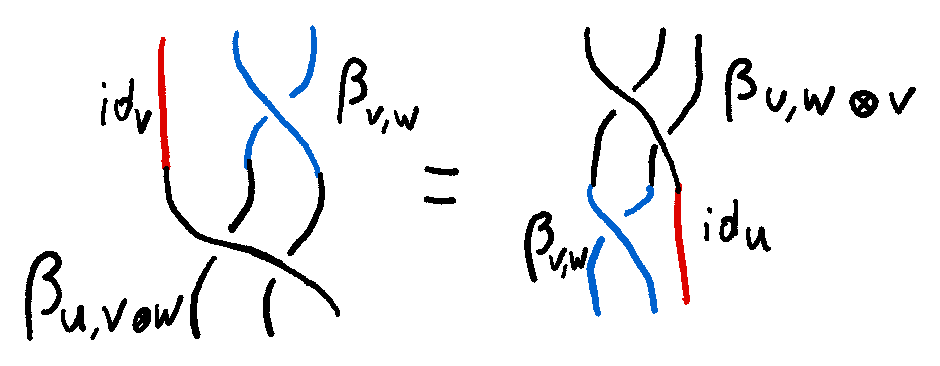
\includegraphics[width=6cm]{images/Lecture 16/stringdiagrams1.png}\]
    we get exactly two specular drawings! However, algebraically, the proof is not finished. We now apply 
    \begin{equation}
        (id_Y \otimes \beta_{X,Z}) \circ (\beta_{X,Y} \otimes id_Z) = \beta_{X,Y\otimes Z}
    \end{equation}
    which inserted for $\beta_{U, V \otimes W}$ and $\beta_{W \otimes V, U}$ gives the result.
\end{proof}

Now, what happens if we take $U=V=W$? Let $\beta:= \beta_{V,V}$, we now get
\begin{equation}
    (\beta \otimes id)\circ (id \otimes \beta)\circ (\beta \otimes id)= (id \otimes \beta) \circ (\beta \otimes id) \circ (id \otimes \beta)
\end{equation}
which is reminiscent of the Yang-Baxter equation (YBE):
\begin{defn}[Yang-Baxter Equation and $R$-matrix]
    Let $V$ be a vector space, $c \in \Aut(V \otimes V)$. The YBE for $c$ is 
    \begin{equation}
        (c \otimes id)\circ (id \otimes c)\circ (c \otimes id)= (id \otimes c) \circ (c \otimes id) \circ (id \otimes c)
    \end{equation}
    A solution to the YBE is called $R$-matrix.

    In coordinates, for $v_i$ a basis of $V$, if
    \begin{equation}
        c (v_i \otimes v_j) = \sum_{k,l} c_{ij}^{kl} v_k \otimes v_l
    \end{equation}
    then the YBE is given by
    \begin{equation}
        \sum_{p,q,y} c_{ij}^{pq}c_{qk}^{yn}c_{py}^{ln}=\sum_{y,q,r}c^{qr}_{jk}c^{ly}_{iq}c^{mn}_{yr}
    \end{equation}
\end{defn}
Theorem \ref{thm:YB_braid} then tells us that, for \textit{any} $V\in\Vect$, $\beta_{V,V}$ is an $R$-matrix.

\begin{ex}
    the automorphism on $V\in\Vect$: $V \otimes V \xrightarrow{swap} V \otimes V$ satisfies the YBE because
    \begin{itemize}
        \item it comes from a standard braiding $\beta$ in $\Vect$
        \item Coxeter relation in $S_3$: $$(12)(23)(12)=(23)(12)(23)$$
    \end{itemize}

    $V$ finite dimensional vector space with basis $e_1, \dots, e_n$ and $q$ an invertible scalar. Now define $c_q (e_i \otimes e_j):= q e_i \otimes e_j $ for $i=j$, $e_j \otimes e_i$ for $i<j$ and $e_j \otimes e_i + (q-q') e_i \otimes e_j$ for $i>j$. A computation then shows that this satisfies the YBE. Note that $c_1 = swap$ is a 1-parameter "deformation" of swap.
\end{ex}

This comes from representation theory!
\begin{defn}
    Let $G$ be a group, a representation of $G$ on $V$ a vector space (or $R$ module) is a group homomorphism $\rho: G \to \Aut(V)$, i.e.
    \begin{equation}
        \rho(gh) = \rho(g) \rho(h), \quad \forall g,h \in G
    \end{equation}
    Now, a morphism of representations $\rho_i: G \to \Aut(V_i), i=1,2$ is a linear map $\alpha: V_1 \to V_2$ such that the following diagram commutes:
    \begin{equation}\label{eq:morphism_of_reps}
        \begin{tikzcd}
            V_1 \ar[r, "\alpha"] \ar[d, "\rho_1(g)"'] & V_2 \ar[d, "\rho_2(g)"]\\
            V_1 \ar[r, "\alpha"'] & V_2 
        \end{tikzcd}
    \end{equation}
    This gives rise to the category of representations of $G$, $\Rep_G$.
\end{defn}
\begin{rem}
    The diagram \ref{eq:morphism_of_reps} looks suspiciously like a natural transformation, and it is! In particular it's exactly example \ref{Cat of representations} in \ref{ex:natural_trafos}. In other words, the category of representations is the functor category:
    \begin{equation}
        \Rep(G) = \Fun(\mathbf B G,\Vect)
    \end{equation}
\end{rem}
\begin{ex}
    Symmetries of a polygon: $G=D_n$ dihedral group and $\rho: D_n \to \Aut(\R^2)$, where $D_n \acts \R^2$ via
     reflections and rotations. For example the reflections can be represented visually for the hexagon as follows
    \[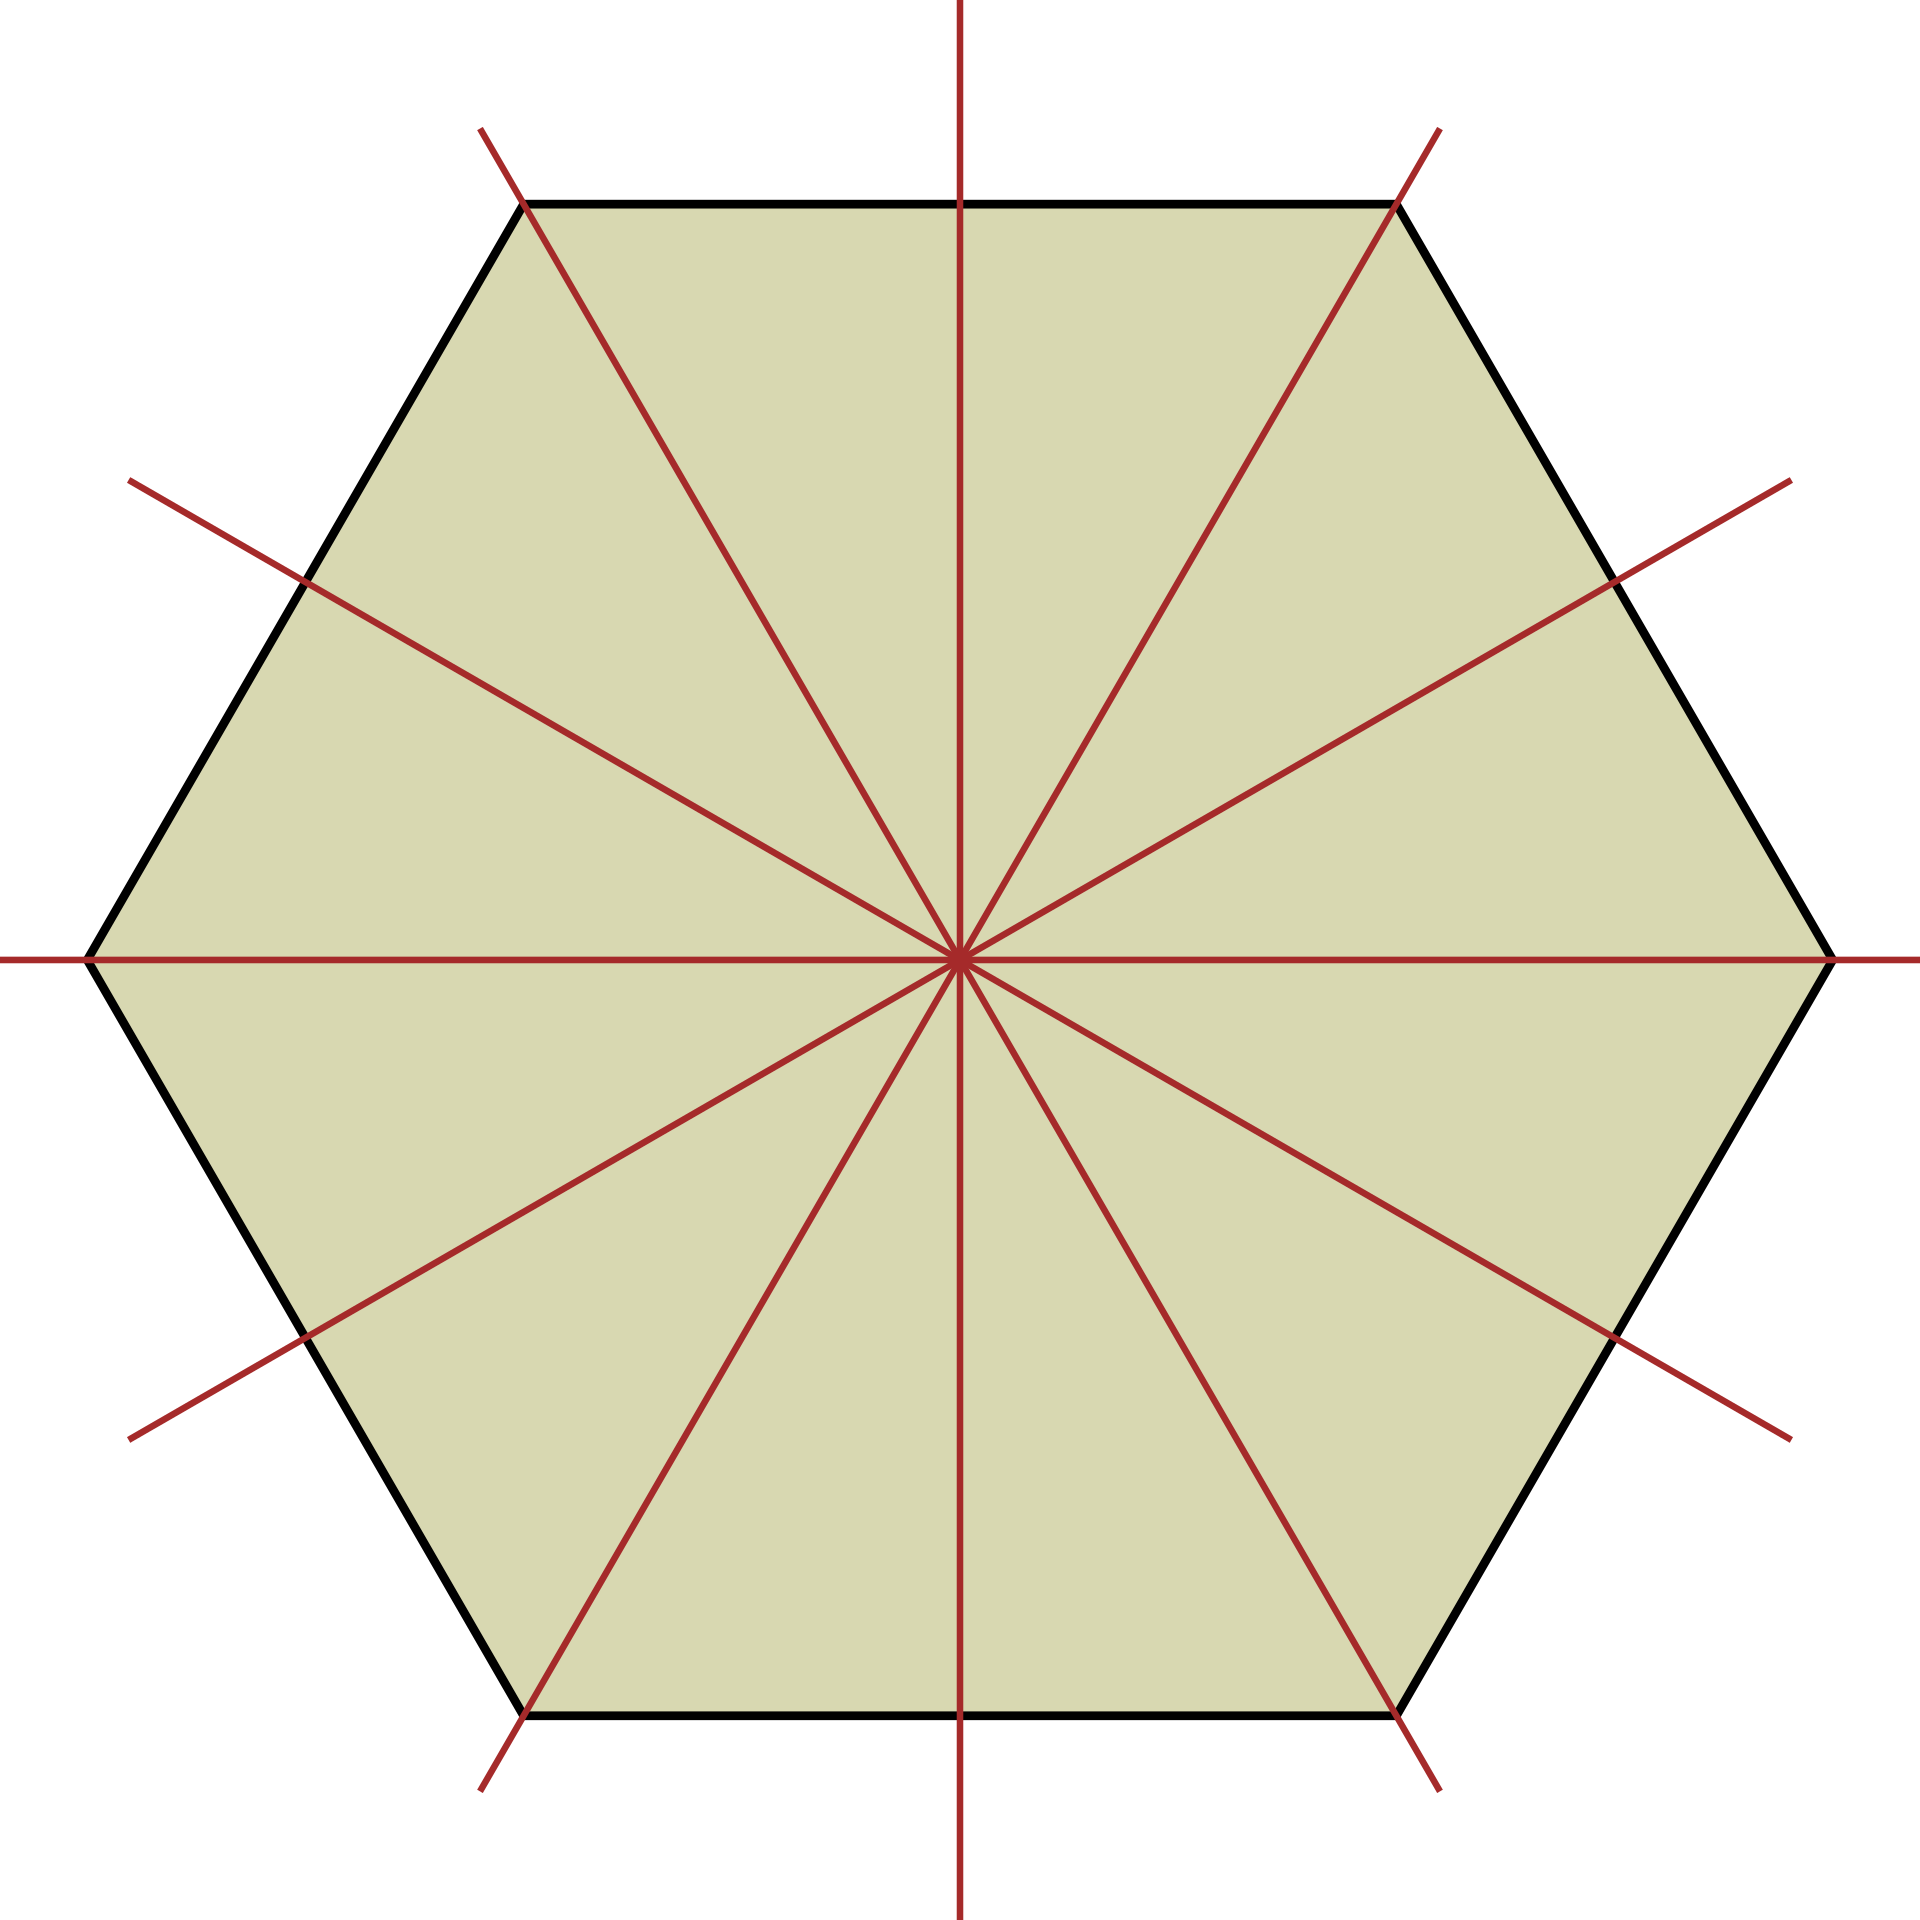
\includegraphics[width=4cm]{images/Lecture 16/Hexagonsymmetries.png}\]
\end{ex}

Solutions of YBE give representations of the braid group, which we explore in the next section.

\subsection{The braid group and the Braid category} % (fold)
\label{ssub:the_braid_group}

\begin{defn}[Braid groups]
\label{defn:braid_group}
    Let $k\geq 3$. The braid group $B_k$ with $k$ strands has $k-1$ generators $\sigma_1, \dots, \sigma_{k-1}$ and 2 relations:
    \begin{flalign}
        \label{eq:braid_relations}
        \quad
        \begin{matrix*}[l]
            1.\;\sigma_i \sigma_j  = \sigma_j \sigma_i &\text{if} \quad |i-j|>1 \\
            2.\;\sigma_i \sigma_{i+1} \sigma_i = \sigma_{i+1} \sigma_i \sigma_{i+1} &\text{if}\quad 1\leq i<k-1 \\
        \end{matrix*}&&
    \end{flalign}
    % \begin{enumerate}
    %     \item $\sigma_i \sigma_j = \sigma_j \sigma_i$ if $|i-j|>1$
    %     \item $\sigma_i \sigma_{i+1} \sigma_i = \sigma_{i+1} \sigma_i \sigma_{i+1}$ for $1\leq i<k-1$
    % \end{enumerate}
    In addition $B_2$ is the free group on one generator $\sigma$, i.e. it is isomorphic to $\Z$. For
    even lower generators $B_1 = B_0 = {e}$.
\end{defn}
\noindent The reason we call $B_k$ the braid group with $k$ strands is that we can picture the elements $\sigma_i$ in the following way:
\[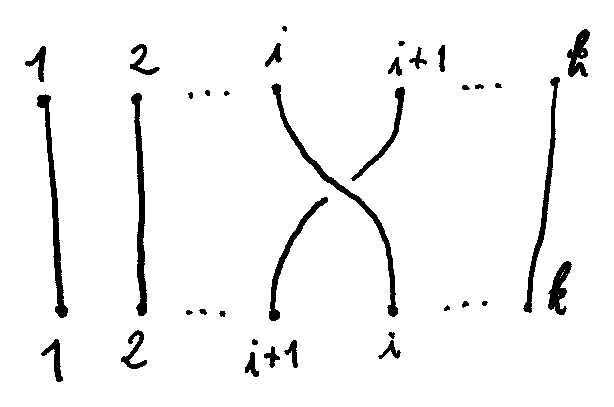
\includegraphics[width=4cm]{images/Lecture 16/BraidGroup.png}\]
which resembles a braid.
\begin{rem}
    There is a surjective homomorphism to the symmetric group
    \begin{equation}
        \begin{tikzcd}[row sep=tiny, column sep=small]
            B_k \ar[r] & S_k \\
            \sigma_k \ar[r, mapsto] & s_k
        \end{tikzcd}
    \end{equation}
    which is clear since $S_k$ has the same generators and relations with in addition $s_i^2=e$.
\end{rem}

\begin{prop}\label{prop:Rmatrix_reptheory}
    Let $c \in \Aut(V \otimes V)$ be an $R$ matrix (i.e. a solution of the YBE). Then, for any $k >0$, there is a unique homomorphism $\rho_k^c: B_k \to \Aut(V^{\otimes k})$ (i.e. a representation of $B_k$ on $\Aut(V^{\otimes k})$) such that
    \begin{equation}
        \rho_k^c (\sigma_i):= c_i, \quad i=1, \dots, k-1
    \end{equation}
    with the $c_i\in \Aut(V^{\otimes k})$ is defined as: take $c$ in position $i, i+1$ and id otherwise, i.e.
    \begin{equation}
        c_i := 
        \begin{cases}
            c \otimes id_{V^{\otimes(k-2)}}, &i=1 \\
            id_{V^{\otimes(i-1)}} \otimes c \otimes id_{V^{\otimes(k-i-1)}}, & 1<i<k-1 \\
            id_{V^{\otimes(k-2)}} \otimes c, & i=k-1    
        \end{cases}
    \end{equation}
    (the second expression alone is enough is we forget about the identity when we have $id_{V^{\otimes 0}}$)
\end{prop}
% so R matrices give us representations of the Braid groups, is the converse also true?
\begin{rem}
    With this notation, YBE reads as 
    \begin{equation}
        c_1 c_2 c_1 = c_2 c_1 c_2
    \end{equation}
    since the extra identities have no relevant effect. Equivalently then the YBE can also be written as 
    \begin{equation}
        c_i c_{i+1} c_i = c_{i+1} c_i c_{i+1}
    \end{equation}
\end{rem}

\begin{proof}
    Define $\rho_k^c (\sigma_i):= c_i$ and check that the $c_i$ satisfy the relations in Definition \ref{defn:braid_group}. 

    \noindent For 1. we would like
    \begin{equation}
        c_j c_i
        = 
        c_i c_j 
    \end{equation}
    for $i > j+1$. This follows from the fact that $c_i$ and $c_j$ don't "interact":
    \begin{align*}
        &
        (id_{V^{\otimes(j-1)}} \otimes c \otimes id_{V^{\otimes(k-j-1)}})
        (id_{V^{\otimes(i-1)}} \otimes c \otimes id_{V^{\otimes(k-i-1)}}) 
        \\
        =&
        (id_{V^{\otimes(j-1)}} \otimes c \otimes id_{V^{\otimes(i-j-2)}}\otimes id_{V^{\otimes 2}} \otimes id_{V^{\otimes(k-i-1)}}) 
        (id_{V^{\otimes(i-1)}} \otimes c \otimes id_{V^{\otimes(k-i-1)}})
        \\
        =&(id_{V^{\otimes(j-1)}} \otimes c \otimes id_{V^{\otimes(i-j-2)}} \otimes c \otimes id_{V^{\otimes(k-i-1)}} )\\
        =&
        (id_{V^{\otimes(i-1)}} \otimes c \otimes id_{V^{\otimes(k-i-1)}}) 
        (id_{V^{\otimes(j-1)}} \otimes c \otimes id_{V^{\otimes(k-j-1)}})
    \end{align*}

    \noindent 2. simply follows from the remark above.
\end{proof}

% -------------------------------------------------------------
% ---------------------- LECTURE 17 10/1 ----------------------
% -------------------------------------------------------------

The braid group is also connected to the concept of configuration space.
%TODO check reference for names...
\begin{defn}[Unordered configuration space]
    Let $\uConf_k(\R^2) \subset (\R^2)^k$ (the ordered configuration space of $\R^2$) be the subspace of $k$-tuples $(x_1, \dots, x_k)$ such that $x_i \neq x_j$ for $i\neq j$.
    Then we have an action $S_k \acts \uConf_k(\R^2)$. 
    The \textit{unordered} configuration space is $\Conf_k(\R^2) := \uConf_k(\R^2)/S_k$.
\end{defn}

% Distinguished configuration... %TODO complete, was this just the choice of p or what /William
\noindent We would like to talk about the fundamental group of $\Conf_k(\R^2)$, but for that we need to pick a basepoint. Let us indicate coordinates by working in \C rather than in $\R^2$. Then let $p = [(1, 2, \dots, k)] \in \C^k$, that is to say that all points are placed on the $x$-axis in steps of 1 (and the square brackets are to indicate the class under the quotient by $S_k$).
\noindent We then have a homomorphism $B \to \pi_1(\Conf_k(\R^2), p)$ which sends $\sigma_i \mapsto \hat \sigma_i = [f_i]$ where $f^i$ is a loop at $p$, defined in $(\R^2)^k$ by:
\begin{equation}
    f^i = (f_1^i, \dots, f_k^i): [0,1] \to (\R^2)^k \cong \C^k
\end{equation}
\begin{align}
    f^i_j(s) &= j, \quad \text{if } j \neq i, i+1 \\
    f^i_i(s) &= \frac{1}{2} (2i+1 - e^{\pi i s}) \\
    f^i_{i+1}(s) &= \frac{1}{2} (2i+1 - e^{\pi i s}) 
\end{align}
this indeed induces a loop in $\Conf_k (\R^2)$.

\noindent For it to be a homomorphism we need to check that the images of $\sigma_i$ satisfy the relations \ref{eq:braid_relations} of the $B_k$ group.
\begin{enumerate}
    \item $\hat\sigma_i \hat\sigma_j = \hat\sigma_j \hat\sigma_i$ for $|i-j|>1$
    \item $\hat\sigma_i \hat\sigma_{i+1} \hat\sigma_i = \hat\sigma_{i+1} \hat\sigma_i \hat\sigma_{i+1}$ for $1\leq i<k-1$
\end{enumerate}
For 1. one finds the same result as in the proof of Proposition \ref{prop:Rmatrix_reptheory} above, i.e. for $|i-j|>1$, $\hat\sigma_i$ and $ \hat\sigma_j$ don't "interact" with one another. Instead 2. can be checked visually.
%DRAWING

\noindent The following important result can be found in \cite{Artin1950}. 
\begin{thm}
    This homomorphism $\phi: B_k \to \pi_1 (\Conf_k(\R^2),p)$ is an isomorphism.
\end{thm}

The drawings above may give us the idea to construct a category in which morphisms are given by the paths $f$ which are morphisms between sets $k$ points. This will be the Braid category.
\noindent More in detail, given a representative $f = (f_1, \dots, f_k): [0,1] \to (\R^2)^k$ of an element in $\pi_1(\Conf_k(\R^2),p)$ we can define the following subset of $[0,1] \times \R^2$:
\begin{equation}
    L_f = \bigcup_{j=1}^k \{(s, f_j(s)): s \in [0,1]\}
\end{equation}
which is pretty much what we were drawing above, the graph of the path considered. It is therefore simply the union of disjoint line segments.
Note now that
\begin{enumerate}
    \item $\de L_f = \{0,1\} \times \{1,2, \dots, k\}$ since the path starts and ends at $p=[(1, 2, \dots, k)]$.
    \item $\forall s \in [0,1]$ we have that $L_f \cap (\{s\} \times \R^2) = k$ points.
    \item $L_f$ is a bordism from $\{1,\dots, k\}$ to itself. Where in addition we can add an orientation by "flowing" from 0 to 1.
    \item group structure gives the composition of bordisms.
    \item always have just $\bullet_1, \dots, \bullet_k$ as source/target $\implies$ can take just this object.
    \item bordism $L_f$ comes with an embedding into $[0,1] \times \R^2$. This really depends on the representative! But the bordism itself only depends on $[f] \in \pi_1(\Conf_k(\R^2))$.
    %DRAWING
\end{enumerate}

\noindent This allows us to define the following category:
\begin{defn}
    The $\Braid$ category is given by:
    \begin{itemize}
        \item objects: natural numbers $0, 1, \dots, k, \dots$, which we think of as sets of $k$ points,
        \item morphisms: 
            \begin{equation}
                 \Hom_{\Braid}(k,l) = 
                 \begin{cases}
                     \emptyset & \text{if } k \neq l \\
                     \text{isotopy classes of "braids" from $k$ to $k$} & \text{if } k = l
                 \end{cases}
                 %& \emptyset\quad \text{if } k \neq l\\
                 %& \text{isotopy classes of "braids" from $k$ to $k$}
             \end{equation} 
             By braids we mean a "permutation 1 bordism together with an embedding" $\bigcup_{\{1, \dots, k\}} [0,1] \hookrightarrow [0,1] \times \R^2$ such that 1. and 2. hold.
             %I think 1. is implied and we only need 2 /William
         \item composition is "stacking the pictures", i.e. composition of bordisms plus stacking embeddings (using $[0,1] \cup_{1=0} [0,1] \cong [0,1]$). 
         \item braided monoidal structure given pictorially by stacking $\R^2$s next to each other, in the sense that $k \otimes l = k+l$ in which the additional $l$ points are simply stacked next to the initial $k$ points. 
         %(using embedding $\R^2 \amalg \R^2 \cong [0,1]^2 \amalg [0,1]^2 \hookrightarrow \R^2 \cong [0,1]^2$).
    \end{itemize}
\end{defn}

\begin{exercise}
    One could now prove that $\Braid \simeq \coprod_{k\geq 0} B_k$, where $\coprod_{k\geq 0} B_k$ was in one of the exercise sheets. 
    %Isomorphism or equivalence of categories? /William
\end{exercise}

\subsection{Expanding the Braid category: the Tangle category} % (fold)
\label{ssub:expanding_the_braid_category_the_tangle_category}

Next step: allow more morphisms, namely all bordisms, together with suitable embeddings.
\begin{defn}
    A tangle with $k$ inputs and $l$ outputs is a 1 dimensional bordism $\Sigma$ from $k$ to $l$ points together with $\Sigma \hookrightarrow [0,1] \times \R^2$ smooth embedding, such that
    \begin{align}
        \de_{in} \Sigma &= \{(0,1), (0,2), \dots, (0,k)\}\\
        \de_{out} \Sigma &=\{(1,1), (1,2), \dots, (1,l)\}
    \end{align}
\end{defn}
%DRAWING example

\noindent We can now define the tangle category, of which $\Braid$ will be a (braided monoidal) subcategory.
\begin{defn}
    The tangle category $\Tang_1$ has:
    \begin{itemize}
        \item objects: natural numbers
        \item morphisms: 
        \begin{equation}
            \Hom_{\Tang_1}(k,l) = \{\text{isotopy classes of tangles from $k$ to $l$ points}\}
            %TODO specify somewhere what we mean by isotopy
        \end{equation}
        \item composition of underlying bordisms and stacking embeddings using $[0,1] \cup_{1=0} [0,1] \hookrightarrow [0,1]$
        \item braided monoidal structure as before
    \end{itemize}
\end{defn}
\noindent Note that we also have $\Braid \subset \Tang_1$.

%I think we already have this def /William
\begin{defn}
    Let $(\cat, \otimes)$ be a monoidal category and $X \in \cat$. We say that $Y$ is a right dual of $X$ if there is 
    \begin{align}
        ev_X&: Y \otimes X \to 1 \\
        coev_X&: 1 \to X \otimes Y
    \end{align}
    such that the snake relations are satisfied. We then say that $X$ is a left dual of $Y$. See \ref{DefDualObj} for a complete defintition.
\end{defn}

\begin{lem}
    In $\Tang$, every object has a left and a right dual.
\end{lem}
\begin{proof}
    Same pictures as for $\Bord_1$.
\end{proof}

% -------------------------------------------------------------
% ---------------------- LECTURE 18 15/1 ----------------------
% -------------------------------------------------------------

%TODO probably already written
% \begin{defn}
%     A tangle with $k$ inputs and $l$ outputs is a one dimensional bordism $\Sigma$ from $k$ points to $l$ points together with a smooth embedding $\Sigma \hookrightarrow [0,1] \times \R^2$ such that
%     \begin{itemize}
%         \item $\de_{in} \Sigma = \{(0,1), (0,2), \dots , (0,k)\}$
%         \item $\de_{out} \Sigma = \{(1,1), (1,2), \dots , (1,l)\}$
%     \end{itemize}
%     This gives a braided monoidal category $\Tang_1 \supset \Braid$.
% \end{defn}
% DRAWING

We can now define the concept of a framing on a tangle, which is different from what we previously meant as framing.
\begin{defn}
    A framing on a tangle  is a nonvanishing normal vector field on the tangle such that at the in-boundary and at the out-boundary it "points up".
\end{defn}
\noindent This definition is made clearer through examples:
\begin{ex}
    ...
    %DRAWING
\end{ex}

Considering framed tangles leads to the \textit{framed} tangle category $\Tang_1^{fr}$.

\noindent In fact, on the line segment as a bordism between two points we have \Z many non isotopic framings corresponding to the \textit{winding number} of normal vector fields. Similarly, $S^1$ also has \Z many framings. 

\noindent We noted last time that $\Tang_1$ has left and right duals, one can check now that $\Tang_1^{fr}$ also does. We see that the framed tangle category is very similar but it has \Z many morphisms between two points, instead of just one. This idea can be generalized with the concept of a ribbon category:
\begin{defn}
    A ribbon category is a braided monoidal category \cat in which:
    \begin{enumerate}
        \item every object $X$ has a right dual $X^\vee$, thus satisfying  $$ev_X : X^\vee \otimes X \to 1$$ $$coev_X: 1 \to X \otimes X^\vee$$ which satisfies the snake relations/triangle identities (\textit{right rigid category}),
        \item there is a pivotal structure, that is a  monoidal isomorphism
        \begin{equation}
            w: id_\cat \implies ( -)^{\vee\vee}
        \end{equation}
        (these two properties are the defining ones for a \textit{pivotal category})
        \item For any object $X$, we have a "twist"
        \begin{equation}
            \vartheta_X = (id \otimes ev_{X^\vee}) \circ (\beta_{X,X} \otimes id) \circ( id_X \otimes coev_X)
        \end{equation}
        This satisfies 
        \begin{equation}
            ((\vartheta_X)^\vee  = \vartheta_{X^\vee}
        \end{equation}
        %this an extra condition right? not just a fact /William
    \end{enumerate}
    Here we're using an abuse of notation, by identifying $X^{\vee \vee}$ with $X$.
%TODO diagram
\end{defn}

\begin{ex}
    In $\Tang_1^{fr}$, the $\vartheta$ is exactly the picture with the blackboard framing. It remains to check property 3, which will be an exercise.
\end{ex}

The definition of the dual of a map $f: X \to Y$ was given in \ref{DualMorph} and is given by the following composition:
$$f^\vee:Y^\vee\xrightarrow{id_{Y^\vee} \otimes coev_X}Y^\vee\otimes X \otimes X^\vee\xrightarrow{id_Y^\vee\otimes f\otimes id_{X^\vee}}Y^\vee\otimes Y\otimes X^\vee\xrightarrow{ev_Y\otimes id_{X^\vee}}X^\vee$$

%TODO maybe add explicit calculation /William

\begin{lem}
    Let \cat be a braided pivotal category. Then every object has a left dual, the twist is invertible and natural in $X$ and $\vartheta_\unit = id_\unit$ and
    \begin{equation}
        \vartheta_{X \otimes Y} = \beta_{Y,X} \circ \beta_{X,Y} \circ \vartheta_X \otimes \vartheta_Y
    \end{equation}
\end{lem}
%I don't know if this was said in class but it was in the script /William
\begin{notat}
    We denote the left dual of $X$ by $({}^\vee X, \tilde{ev_X}, \tilde{coev_x})$.
\end{notat}

\begin{ex}
\hfill
    \begin{itemize}
        \item $\Vect_k^{finite dim}$ is a ribbon category with the usual tensor product and braiding.
        \item $\Mod_R^{fpp} = R-\Mod^{fpp}$ is a ribbon category, where $fpp$ stands for finitely presented and projective and $R$ is a ring or $k$ algebra.
    \end{itemize}
    However both these examples are \textit{symmetric} monoidal
\end{ex}
\noindent We would also like some more examples which are braided but \textit{not} symmetric.

%so here we mean algebra over a ring while before was algebra over field? Or what's the difference /William
\noindent In order to do so, consider an algebra $A$, then $A-\Mod$ is a category. Now, which extra structure on $A$ guarantees that $A-\Mod^{f.d.}$ is ribbon? Section \ref{ssub:making_} below is dedicated to answering this question. As a small preview we will be dealing with:
\begin{itemize}
    \item representations of "quantum groups":
    \begin{itemize}
        \item a "deformation" of $\Rep G = \Mod U\g$, %why is this true?/William
        \item equivalently, a deformation of $U\g$ as a "Hopf algebra";
    \end{itemize}
    \item representations of a "ribbon Hopf algebra" $H$ which is a Hopf algebra with additional structure. We'll find $H-\Mod^{f.d.}$ to be a ribbon category. In particular we'll concentrate on $G=SL_2$ and we take $H = U_q (\sl_2)$ where $q$ is a root of unity.
\end{itemize}

Before that, we define a variation of the tangle category above and we'll have an interlude on knot theory.
\begin{defn}
    Let \cat be a ribbon category. $\Tang_1^{fr}(\cat)$ is the following ribbon category, in which we "decorate with objects in \cat".
    \begin{itemize}
        \item objects: finite sequences
            \begin{equation}
                (V_1, \epsilon_1), \dots, (V_k, \epsilon_k)
            \end{equation}
            where $V_i \in \cat$ and $\epsilon_i = \pm 1$. This corresponds to $k$ points in $\Tang_1^{fr, or}$ in which $\epsilon$ gives us the orientation of each point.
        \item morphisms: has underlying (isotopy classes of) framed oriented tangles + each component is labelled by $V \in \cat$ such that the source and target are labelled by $(V, \pm 1)$.
        \item Composition is stacking pictures but only if the labels match up.
    \end{itemize}
    The "correspondence" above is actually a forgetful functor $\Tang_1^{fr}(\cat) \to \Tang_1^{fr, or}$, in which $or$ means adding an orientation to the bordism.
\end{defn}

\begin{prop}
    If \cat is a ribbon category, then there is a unique braided monoidal functor $F : \Tang_1^{fr} (\cat) \to \cat$ such that
    \begin{itemize}
        \item $F(V, +1) = V$ and $F(V, -1) = V^\vee$
        \item $\forall V, W \in \cat$ we have:
        %DRAWING
    \end{itemize}
\end{prop}

Finally, what does all this have to do with 3d TFTs? 
% https://q.uiver.app/#q=WzAsNCxbMCwwLCJcXFRhbmdee1xcZnJ9X3sxfShcXGNhdCkiXSxbMCwyLCJcXEJvcmRfezN9Il0sWzEsMCwiXFxjYXQiXSxbMiwwLCJcXFZlY3QiXSxbMCwxLCJcXG9wZXJhdG9ybmFtZXtzdXJnZXJ5IH0iLDIseyJzdHlsZSI6eyJ0YWlsIjp7Im5hbWUiOiJhcnJvd2hlYWQifSwiYm9keSI6eyJuYW1lIjoic3F1aWdnbHkifX19XSxbMCwyXSxbMiwzLCJmb3JnZXQiXSxbMSwzXV0=
\[\begin{tikzcd}[cramped]
	{\Tang^{\fr}_{1}(\cat)} & \cat & \Vect \\
	\\
	{\Bord_{3}}
	\arrow["{\operatorname{surgery }}"', squiggly, tail reversed, from=1-1, to=3-1]
	\arrow[from=1-1, to=1-2]
	\arrow["forget", from=1-2, to=1-3]
	\arrow[from=3-1, to=1-3]
\end{tikzcd}\]
We will use:
\begin{itemize}
    \item every 3 manifold arises from framed 1-tangles via \textit{surgery},
    \item two tangles giving the same 3 manifold can be related by \textit{Kirby moves},
    \item $F_\cat$ is invariant under Kirby moves if \cat is a \textit{modular} tensor category.
\end{itemize}

% -------------------------------------------------------------
% ---------------------- LECTURE 19 22/1 ----------------------
% -------------------------------------------------------------

\subsection{Interlude on knots, links and the Kones polynomial} % (fold)
\label{sub:interlude_on_knots_links_and_the_kones_polynomial}

\begin{ex}

    Examples of knots are the following:
    \begin{itemize}
        \item the \textit{unknot} \[\includegraphics[width=2.5cm]{images/Lecture 19/unknot.png}\]
        \item the \textit{trefoil} \[\includegraphics[width=2.5cm]{images/Lecture 19/trefoil.png}\]
        \item the \textit{figure 8 knot} \[\includegraphics[width=2.5cm]{images/Lecture 19/unknot.png}\]
        
    \end{itemize}
    and of links:
    \begin{itemize}
        \item the \emph{Hopf link}  \[\includegraphics[width=2.5cm]{images/Lecture 19/Hopflink.png}\]
        \item the \emph{Borromean rings}  \[\includegraphics[width=2.5cm]{images/Lecture 19/Borromeanrings.png}\]
    \end{itemize}
\end{ex}
\begin{rem}[Knots and links as symbols \extra]
The Borromean rings are called 'Borromean' because they appear on the coat of arms of a noble family from Northern
Italy named 'Borromeo'. However, this is not the only instance of such link in history. They often appear elswhere
 with fascinating symbolism. For instance,
 they also symbolized the trinity
\[\includegraphics[width=2.5cm]{images/Lecture 19/BorromeanRings-Trinity.png}\]
Interlocked triangles, which we now refer
to as 'valknut', often appear in areas inhabited by Germanic peoples. Sometimes the valknut symbolizes the pagan
 God Odin. 
Some of these valknuts are topologically equivalent to the Borromean rings, such version is called the tricursal
 valknut. 
 Here is an example of a tricursal valknut on an 
ornate slab of stone in
 Sweden called the Stora Hammars I.

\[\includegraphics[width=2.5cm]{images/Lecture 19/ValknutStoraHammars.png}\]

Another version of the valknut called the unicursal valknut is not topologically equivalent to the Borromean link:
 it is a knot and ambient isotopic to
 the trefoil. It is the current symbol of the German Football
 Association.
 \[\includegraphics[width=2.5cm]{images/Lecture 19/DFB_Logo.png}\]
\end{rem}
\begin{defn}
    A link is a finite collection of circles smoothly embedded in $\R^3$: 
    \begin{equation}
        \coprod_{i=1}^k S^1 \hookrightarrow \R^3
    \end{equation}
\end{defn}
In which smoothness is to exclude some pathological situations. For instance the following one
 \[\includegraphics[width=6.6cm]{images/Lecture 19/pathological.png}\]
 This is pathological because it should be intuitively be equivalent to the unknot and to show this we would need 
 infinitely many Reidemeister moves of type 1 (see \ref{moves}) to deform it to the unknot. 
 However, one the fundamental theorem of knot theory \ref{ReidemeisterTHM}
 manages to prove that two knots are equal if one can be deformed into the other with \emph{finitely} many 
 Reidemeister moves.
\begin{defn}
    A knot is a link with one component ($k=1$).
\end{defn}

\begin{defn}
    Two links $L_1, L_2: \amalg_{i=1}^k S^1 \hookrightarrow \R^3$ are equivalent if there exists an ambient isotopy between them, i.e. $H: \R^3 \times [0,1] \to \R^3$ such that
    \begin{itemize}
        \item $H(-,0) = id$
        \item $\forall t \in [0,1], \; H(-,t)$ is a diffeomorphism
        \item $H(-,1) \circ L_1 = L_2$
    \end{itemize}
\end{defn}

A goal of knot theory is to find an invariant of knots/links, i.e. an assignment
\begin{equation}
    \{\text{knots/links}\} \to \R, \Z[A,A^{-1}],\dots
\end{equation}
such that if two links are equivalent we get the same number, polynomial, $\dots$.

A link invariant is complete if it detects when 2 links are/are not equivalent.

Concretely, we represent links and nots by 2d drawings, these drawings are called \textit{Link diagrams}. Let $L$ be a link and $p:\R^3 \to \R^2$ a projection.
\begin{defn}
    $p(L)$ is regular if 
    \begin{enumerate}
        \item every point has at most 2 preimages in $L$
        \item intersections are transversal
    \end{enumerate}
\end{defn}
\begin{defn}
    A link diagram is a regular $p(L)$ together with over/under information at each crossing. Visually:
     \[\includegraphics[width=4.6cm]{images/Lecture 19/regularproj.png}\]
\end{defn}
\begin{rem}
    Given a link, we do \textit{not} always get a link diagram $p(L)$, but we can always deform/perturb the embedding $L: \coprod_{i=1}^k S^1 \hookrightarrow \R^3$ by ambient isotopy to $L'$ which gives a link diagram. 
    For instance, the following two projections are irregular: 
     \[\includegraphics[width=6.6cm]{images/Lecture 19/irregularproj.png}\]
     But such situation could be avoided by moving such links in a reasonable manner via ambient isotopies.
\end{rem}

Our aim is to define a knot/link invariant by defining something on link diagrams. 
In order to do this we introduce Reidemeister moves, which are the following local changes in a link diagram:
\begin{itemize}\label{moves}
    \item (I or R1) \[\includegraphics[width=4.6cm]{images/Lecture 19/R1.png}\]
    \item (II or R2) \[\includegraphics[width=4.6cm]{images/Lecture 19/R2.png}\]
    \item (III or R3) \[\includegraphics[width=4.6cm]{images/Lecture 19/R3.png}\]
\end{itemize}

\begin{thm}[Reidemeister]\label{ReidemeisterTHM}
    Two links are equivalent if and only if their link diagrams are the same up to finitely many Reidemeister
     moves and isotopies in $\R^2$. 
\end{thm}
This theorem is very important because it tells us that the link diagrams have all the information of the
 equivalence class of the link, so to determine (in)equivalence we can work with link diagrams.

A first knot invariant is the "number of tricolorings": we color a link diagram with three colors according to the following rules
\begin{itemize}
    \item each strand is one color
    \item at each crossing either all three strands are the same color, or they're all different.
\end{itemize}
\begin{ex}
    There are always three trivial colorings, the monochromatic ones. For the unknot, these are the only three tricolorings
    \[\includegraphics[width=5cm]{images/Lecture 19/Unknotcolors.png}\]
    while the trefoil has an additional one:
   \[\includegraphics[width=7cm]{images/Lecture 19/Trefoilcolors.png}\]

    This shows that the trefoil knot is \textit{not} equivalent to the unknot.
\end{ex}
In order to prove that this is a knot invariant one should check that it is invariant under Reidemeister moves.

We now finally get to the Jones polynomial, found by Jones in 1984, and this presentation is from Kauffmann in 1987. The motivation for it comes from operator algebras and the braid group representations. 
\begin{defn}
    The Kauffmann bracket of a link diagram $D$ is a Laurent polynomial $\langle D\rangle \in \Z[A,A^{-1}]$ defined by
    \begin{itemize}
        \item $\langle \includegraphics[width=0.4cm]{images/Lecture 19/unknot.png}\rangle = 1$
        \item $\langle \includegraphics[width=0.4cm]{images/Lecture 19/cross.png}\rangle=A\cdot\langle \includegraphics[width=0.4cm]{images/Lecture 19/1Kauffmann.png}\rangle + A^{-1}\cdot\langle \includegraphics[width=0.4cm]{images/Lecture 19/2Kauffmann.png}\rangle $
        \item $\langle L\cup \includegraphics[width=0.4cm]{images/Lecture 19/unknot.png}\rangle=(-A^{2}-A^{-2})\langle L\rangle$
    \end{itemize}
\end{defn}
\begin{ex}
   $$\langle\includegraphics[width=0.7cm]{images/Lecture 19/ooHighlighted.png}\rangle= A\cdot\langle \includegraphics[width=0.7cm]{images/Lecture 19/oo1Kauffmann.png}\rangle + A^{-1}\cdot\langle \includegraphics[width=0.7cm]{images/Lecture 19/oo2Kauffmann.png}\rangle =$$
   $$=A(-A^{2}-A^{-2})\langle\includegraphics[width=0.4cm]{images/Lecture 19/unknot.png}\rangle + A^{-1}\langle\includegraphics[width=0.4cm]{images/Lecture 19/unknot.png}\rangle=$$
   $$=-A^3-A^{-1}+A^{-1}=-A^3$$
   There is an issue:
   $$\langle\includegraphics[width=0.7cm]{images/Lecture 19/oo.png}\rangle=\langle\includegraphics[width=0.55cm]{images/Lecture 19/Laststepkauffmann.png}\rangle$$
   and the last image is equivalent to the unknot, with an application of the first Reidemeister move, but
   $$\langle\includegraphics[width=0.55cm]{images/Lecture 19/Laststepkauffmann.png}\rangle=A^3$$
   and 
   $$\langle \includegraphics[width=0.4cm]{images/Lecture 19/unknot.png}\rangle = 1$$
   \end{ex}
This shows that the Kauffmann bracket is \textit{not} a knot invariant, in particular it is not invariant under R1. It \textit{is} however invariant under R2 and R3, in fact the coefficients in the definition of the bracket are exactly the ones that preserve R2 and R3.

From now on: links are oriented, meaning $S^1$ comes with an orientation. So we can talk about oriented link invariants, for which we have oriented Reidemeister moves. 

Now we would like to fix the problem with the Kauffmann bracket. 
\begin{defn}
    The sign of a crossing is 
    %DRAWING
\end{defn}
\begin{defn}
    The writhe of an oriented link diagram $D$ is the sum of the signs of the crossings:
    \begin{equation}
        w(D) = \sum_{c \text{ crossing in } D} \sign(c)
    \end{equation}
\end{defn}

\begin{lem}
    The writhe is also invariant under R2 and R3, and changes under R1 as ...
    %DRAWING
\end{lem}

\begin{defn}
    For any link $L$, define $\chi (L) = (-A^3)^{-w(p(L))} \langle p(L)\rangle \in \Z[A^{-1},A]$
\end{defn}
\begin{thm}
    This is a link invariant.
\end{thm}

\begin{ex}
    Hopf link vs two detached links
    %DRAWING
\end{ex}

\begin{defn}
    For any unoriented link $L$, the Jones polynomial of $L$ is 
    \begin{equation}
        V(L) = \chi(L)|_{A=t^{1/4}} \in \Z[t^{-1/2},t^{1/2}]
    \end{equation}
\end{defn}

\begin{ex}
    trefoil %TODO complete

    $V(D) = t+t^3-t^4$
\end{ex}

% -------------------------------------------------------------
% ---------------------- LECTURE 20 24/1 ----------------------
% -------------------------------------------------------------

Observe
\begin{itemize}
    \item $V(unknot) = 1$
    \item skain relation: if $L_+, L_-, L_0$ are the same link except for at one crossing, according to the following picture
    %DRAWING

    then 
    \begin{equation}
        t^{-1}V(L_+) -tV(L_-) + (t^{-1/2} - t^{1/2}) V(L_0) = 0
    \end{equation}
\end{itemize}

Explanation of problem of the Kauffmann bracket with R1:
\begin{defn}[Alternative]
    A framed link is (a link together with a nonvanishing normal vector field as before) the image of a smooth embedding of $\coprod_{i=1}^k S^ \times [0,1] \hookrightarrow \R^3$.
\end{defn}
\begin{rem}
    This can be projected onto $\R^2$ such that annuli are "flat", this is the "blackboard framing" from previously.
\end{rem}
\begin{ex}
    We can give two framings on the unknot which are not equivalent:
    %DRAWING
\end{ex}
\begin{thm}
    $L,L'$ framed links, $D,D'$ diagrams thereof using blackboard framings. Then $L \sim L'$ (isotopy equivalence with framing) if and only if $D$ is related to $D'$ via R2, R3 and the modification of R1 given by
    %DRAWING
\end{thm}
\begin{thm}
    The Kauffmann bracket is a framed link invariant.
\end{thm}
Recall we had $\Tang_1^{or,fr}(\cat) \to \cat$ where \cat is a ribbon category. Now, fix a $V \in \cat$, we get an injection $\Link^{or,fr} \hookrightarrow \Tang_1^{or,fr}(\cat)$ in which we decorate each strand (component) by $V$. The goal is then to find a specific ribbon category \cat such that we get back the Jones polynomial. We'll find $\cat = U_q\sl_2 -Mod^{f.d.}$.


\subsection{Making \texorpdfstring{$A-\Mod^{f.d.}$}{A-Mod f.d.} into a ribbon category} % (fold)
\label{ssub:making_}

%Back to algebra: How to get a ribbon category?
We now want to add additional structures on an algebra $A$ in such a way that $A-\Mod^{f.d.}$ becomes a ribbon category.
%why do we want to do this?
We therefore need $A-\Mod^{f.d.}$ to have the following structures:
\begin{itemize}
    \item monoidal structure,
    \item existence of (right) duals (right rigidity),
    \item braiding,
    \item pivotal structure,
    \item twist,
\end{itemize}
which we gradually construct in this order. 

\subsection*{Monoidal structure} % (fold)

In order to do this, we will need additional structures on $A$, starting with the following.
\begin{defn}
    A Hopf algebra in a braided strict monoidal category \cat is 
    \begin{itemize}
        \item a bialgebra $(H,\mu,\eta,\Delta,\epsilon)$, in which we represent all these maps as the following drawings
        %DRAWING

        These maps should satisfy
        \begin{equation}
            (\mu \otimes \mu) \circ( id \otimes \beta \otimes id) \circ (\Delta \otimes \Delta) = \Delta \circ \mu
        \end{equation}
        and
        %TODO complete
        \item antipode map $S: H \to H$ depicted as 
        %DRAWING

        satisfying
        %DRAWING
    \end{itemize}
\end{defn}
\begin{ex}
    \item Take $H = k[G]$, 
    \begin{equation}
        \begin{matrix}
            \mu(g,h) = gh\quad & \eta(1) = 1\quad & \\
            \Delta(g) = g \otimes g\quad & \epsilon(g) = 1\quad & s(g)  = g^{-1} 
        \end{matrix}
    \end{equation}
    \item for Lie algebra \g, let $U\g$ be its universal enveloping algebra, which we will define shortly. We then have
    \begin{equation}
        \Rep^{f.d.} G \simeq U\g-\Mod^{f.d.}
    \end{equation}
    we will then "deform" this in one of the exercises.
\end{ex}

Recall that a Lie algebra is defined as follows.
\begin{defn}
    A Lie algebra is a vector space with a bilinear map $[-,-]: \g \otimes \g \to \g$, sending $x \otimes y \mapsto [x,y]$, called the Lie bracket, satisfying:
    \begin{itemize}
        \item anticommutativity: $[x,x]=0$ or $[x,y] = -[y,x]$
        \item Jacobi identity: $[x,[y,z]] + [y,[z,x]] + [z,[x,y]] = 0$
    \end{itemize}
    A homomorphism of Lie algebras $\g, \mathfrak h$ is a linear map $\phi: \g \to \mathfrak h$ such that $\phi([x,y]_\g) = [\phi(x), \phi(y)]_{\mathfrak h}$.
\end{defn}
\begin{ex}
\hfill
    \begin{enumerate}
        \item $\g = \End(V) = \gl_V$, with bracket given by the commutator $[f,g] = f \circ g - g \circ f$. There is also a sub Lie algebra $\sl_V:=\{f \in \gl_V : \tr f = 0\}$.

        If for example we take $V = \R^2$ we have $\gl_2 = \Mat_{2,2}$ and $\sl_2 = \{A \in \Mat_{2,2}: \tr A = 0\}$.
        \item Let $A$ be an associative algebra, then if we take the underlying vector space, with bracket given by the commutator, we get a Lie algebra. In other words, there is a forgetful functor:
        \begin{equation}
            \Alg \to \Lie
        \end{equation}
        and its left adjoint is the concept of universal enveloping algebra which we will see more explicitly later on.
        \item %TODO complete
        \item smooth vector fields on a smooth manifold: $\mathfrak{X} = \Der(\C^\infty(M))$ %TODO weird letter
    \end{enumerate}
\end{ex}
Outlook: in physics we like to look at Lie groups, a smooth manifold with a group structure (i.e. a group object in the category of smooth manifolds). Since it's a manifold, we can look at its tangent space. The Lie algebra $\g$ of $G$ is defined as $T_e G$. %left invariant vector fields....

Now, fix \g a Lie algebra.
\begin{defn}
    The tensor algebra of \g is the (graded) algebra given by:
    \begin{equation}
        T(\g) := \bigoplus_{n=0}^\infty \g^{\otimes n}
    \end{equation}
    with $\g^{\otimes n} \otimes \g^{\otimes k} \to \g^{\otimes(n+k)}$.

    There is a 2 sided ideal $I(\g) \subset T(\g)$ generated by $\langle x \otimes y - y \otimes x - [x,y] \rangle$. We can then define the universal enveloping algebra of \g:
    \begin{equation}
        U\g := T(\g)/I(\g)
    \end{equation}
\end{defn}
The universal enveloping algebra has the universal property that given an algebra $A$ and a Lie algebra map $\g \to A$ there is a unique map $U \g \to A$ making the following diagram commute
\begin{equation}
    \begin{tikzcd}[nodes in empty cells=true]
        \g \ar[dr]\ar[r] & U\g \ar[d, dashed] \\
        & A
    \end{tikzcd}
\end{equation}

\begin{clm}
    $U\g$ is a Hopf algebra, with coalgebra structure given by:
    \begin{itemize}
        \item $\Delta: U\g \to U\g \otimes U\g$ %TODO complete
        \item $\epsilon: U\g  \to k$
        \item $S: U\g \to U\g$
    \end{itemize}
\end{clm}
In general, we'll now see that if $A$ is a Hopf algebra, then $A-\Mod^{f.d.}$ is a monoidal category with duals.

\begin{thm}
    Let $(A,\mu,\eta)$ be a unital associative algebra and $\Delta:A \to A \otimes A, \epsilon:A \to k$ linear maps. Then $(A,\mu,\eta, \Delta, \epsilon)$ is a bialgebra if and only if $(A-\Mod, \otimes , (k,\epsilon))$ is monoidal.
\end{thm}
\begin{itemize}
    \item Let $M,N$ be $A-$modules, then the vector space $M\otimes N$ is an $A-$module via 
    \begin{equation}
        \begin{tikzcd}
            A \ar[r, "\Delta"] & A \otimes A \ar[r] & \End(M) \otimes \End(N) \ar[r] & \End(M \otimes N)
        \end{tikzcd}
    \end{equation}
    \item $(k,\epsilon)$ is an $A-$module via
    \begin{equation}
        A \xrightarrow{\epsilon} \End(k) \cong k
    \end{equation}
    \item associators and unitors are those from $\Vect$.
\end{itemize}

\subsection*{Rigidity} % (fold)

%Schweigert cor 2.5.17 says kind of the opposite, I ALWAYS have a right dual and only have a left dual if S is invertible
\begin{prop}\label{prop:Hopf2}
    Let $H$ be a Hopf algebra and $M$ an $H-$module, then $M^\vee:=\Hom(M,k)$ has an $H$ action via the transpose of $S$, i.e. given $\phi \in \Hom(M,k),\,a \in H$ we get $a \cdot \phi \in \Hom(M,k)$ given by
    \begin{equation}\label{eq:dual_mod_struct}
        (a \cdot \phi) (m):= \phi(s(a) \cdot m)
    \end{equation}
    This is a left dual if $M$ is finite dimensional.
    Now, if $S$ is invertible, ${}^\vee M = \Hom(M,k)$ with $(a \cdot \phi)(m) := \phi(s^{-1}(a)\cdot m)$ is a right dual if $M$ is finite dimensional.
\end{prop}

\begin{cor}
    If $H$ is a Hopf algebra with $S$ invertible, then $H-\Mod^{f.d.}$ is rigid monoidal.
\end{cor}
\begin{proof}[Idea of proof of Proposition \ref{prop:Hopf2}]
    Check that $ev_M, coev_M$ exhibiting dual in $\Vect$ are $H-$module maps.
\end{proof}

% Outlook: To get a ribbon category we need:
% \begin{itemize}
%     \item braiding
%     \item pivotal structure
%     \item twist
% \end{itemize}

% -------------------------------------------------------------
% ---------------------- LECTURE 21 29/1 ----------------------
% -------------------------------------------------------------

\subsection*{Braiding} 
Recall: we want a ribbon category and we had a Hopf algebra, so we had a monoidal category with duals.

We're now using \cite{SchwHopfQuantumTFT} as a reference.

\begin{defn}
    A quasi-triangular structure on a bi/Hopf algebra is a "universal $R$-matrix", i.e. an invertible element $R \in A \otimes A$ such that $\forall x \in A$ with 
    \begin{equation}
        \begin{tikzcd}
            \Delta^{coop}: A \ar[r, "\Delta"] & A \otimes A \ar[r, "\tau_{A,A}"] & A \otimes A
        \end{tikzcd}
    \end{equation}
    the following are satisfied
    \begin{enumerate}
        \item $\Delta^{coop}(x) R  = R \Delta(x)$, and
        \item In $A^{\otimes 3}$ we have 
        \begin{align}
            (\Delta \otimes id_A)(R) = R_{13} R_{23} 
        \end{align}
        \item 
        \begin{equation}
            (id_A \otimes \Delta)(R) = R_{13} R_{12}
        \end{equation}
        in which $R_{12} = R \otimes 1, R_{23} = 1 \otimes R, R_{13} = (\tau_{A,A} \otimes id_A)(1 \otimes R)$
    \end{enumerate}
\end{defn}

\begin{ex}
    Any cocommutative bi/Hopf algebra has a canonical $R$ matrix, $R = 1\otimes 1$, since the first relation simply becomes $\Delta = \Delta^{coop}$, which is exactly the cocommutativity.
\end{ex}

\begin{prop}[4.2.3. in \cite{SchwHopfQuantumTFT}]
    Let $A$ be a bialgebra. Then a braiding on $A-\Mod^{(f.d.)}$ uniquely determines a quasitriangular structure on $A$ and viceversa. 
    % This is what we're trying to do: add structures on A so that A-Mod has more structure.
\end{prop}

\begin{proof}[Proof strategy: ]
    Given a braiding $\beta$, define the universal $R$ matrix to be
    \begin{equation}
        R:=\tau_{A,A}(\beta_{A,A}(1_A \otimes 1_A))
    \end{equation}
    in which $\tau_{A,A}$ is the flip and $\beta_{A,A}$ is the braiding. Then one can check properties 1. 2. and 3. above. 

    Now, the following is also true:
    \begin{clm}
        Given $R$ as above, the braiding can be recovered as follows: $\beta_{U,V} (u \otimes v) = \tau_{U,V}(R(u \otimes v))$, for arbitrary $U, V \in A-\Mod$.
    \end{clm}
    So this motivates that if we are given a universal $R$ matrix, we should define $\beta$ as such, and one should check that it's actually a braiding.
\end{proof}

We're now using \cite{tingley2015minus} as a reference.
Main example: $U_q\sl_2$, Hopf algebra, not cocommutative but has a universal $R$ matrix. Therefore $U_q\sl_2 - \Mod$ is braided monoidal. We get $U_q\sl_2$ from the cocommutative Hopf algebra $U\sl_2$ by "deforming" it.

$U_q\sl_2$ is a $\C(q)$-algebra generators $E,F,K,K^{-1}$ with relations:
\begin{align*}
    KK^{-1} &= K^{-1}K = 1 \\
    KEK^{-1} &= q^2 E \\
    KFK^{-1} &= q^{-2}F \\
    [E,F] &= \frac{K - K^{-1}}{q - q^{-1}}
\end{align*}
We have an important 2 dimensional module ("representation") for $U_q\sl_2$: $V_1 \cong \C^2$ with basis $v_1, v_{-1}$. Now, how does $U_q\sl_2$ act? In this basis we write:
\begin{align*}
    E &=
    \begin{pmatrix}
        0 & 1 \\
        0 & 0 
    \end{pmatrix} \\
    F &= 
    \begin{pmatrix}
        0 & 0 \\
        1 & 0 
    \end{pmatrix} \\
    K &= 
    \begin{pmatrix}
        q & 0 \\
        0 & q^{-1} 
    \end{pmatrix} 
\end{align*}

We also claimed there was a Hopf algebra structure, which we now make explicit. The comultiplication is given by
\begin{align*}
    \Delta(E) &= 1\otimes E + E \otimes K \\
    \Delta(F) &= K^{-1} \otimes F + F \otimes 1 \\
    \Delta(K) &= K \otimes K \\
    \Delta(K^{-1}) &= K^{-1} \otimes K^{-1}
\end{align*}
the counit map:
\begin{align*}
    \epsilon(E) &= \epsilon(F) = 0 \\
    \epsilon(K) &= \epsilon(K^{-1}) = 1
\end{align*}
and we should check that these satisfy the required relations. In addition we need the antipode map:
\begin{align*}
    S(E) &= -EK^{-1}\\
    S(F) &= -KF \\
    S(K) &= K^{-1} \\
    S(K^{-1}) &= K
\end{align*}
We then get the monoidal category $U_q \sl_2-\Mod$. If $U,V$ are objects in $U_q \sl_2-\Mod$, then so is $U\otimes V$ in which we have
\begin{equation}
    E(u \otimes v) = E_U \otimes K_V + U \otimes E_V
\end{equation}
It is also braided... %TODO complete

From $S$ we get the dual of $V_1$: as vector space $V_1^\vee = \Hom(V_1, \C)$, in which $\hat v_1, \hat v_{-1}$ is the dual basis. This has a $U_q \sl_2-\Mod$ structure given by Equation \ref{eq:dual_mod_struct}.

Up to now we therefore get the following correspondence between the structures on $A$ and those on $A-\Mod^{f.d.}$:
\begin{center}
\begin{tabular}{ccc}
bialgebra &$\leftrightarrow$& monoidal \\
Hopf algebra &$\leftrightarrow$& right rigid \\
Hopf with $S$ invertible &$\leftrightarrow$& rigid \\
quasi-triangular &$\leftrightarrow$& braiding 
\end{tabular}
\end{center}


% -------------------------------------------------------------
% ---------------------- LECTURE 22 5/2 -----------------------
% -------------------------------------------------------------

%Tingley a minus sign... https://arxiv.org/abs/1002.0555
%recollection...

Let's make explicit the dual representation to $V_1$, $V_1^\vee = \Hom(V, \C) = \langle \hat v_1, \hat v_{-1}\rangle$, where $\hat v_1$ and $\hat v_{-1}$ are the dual basis.

Recall that we had the \textit{decorated} tangle category. Let's take $\cat = U_q\sl_2 - \Mod^{f.d.}$ and let $V=V_1$ the representation above. In particular we work with "$\Tang_1^{fr,or}(V_1)$"$\subset \Tang_1^{fr,or}(\cat)$ in which we decorate everything with just $V_1$.

\begin{rem}
    \begin{itemize}
        \item $A = q^{-1/2}$
        \item slightly different normalization: $F(unknot) = -q -q^{-1}$.
        \item What about the third relation of the Kauffmann bracket? It follows from monoidality!
    \end{itemize}
\end{rem}

\section{Outlook: How to get a 3D TFT?} % (fold)
\label{sec:outlook_how_to_get_a_3d_tft_}

\subsection{From knots to 3 manifolds: surgery} % (fold)
\label{sub:from_knots_to_3_manifolds_surgery}

Given: a framed link $L\subset S^3$ (so far $L\subset\R^3$ but we now embed that into $S^3$) with $m$ components $L= L_1 \cup \dots \cup L_m$ with $L_i \cong S^1$. Now:
\begin{itemize}
    \item Choose closed tubular neighborhood $U \subset S^3$ of link $L$ such that $U = U_1 \amalg \dots \amalg U_m$:
        \begin{equation}
            \begin{tikzcd}
                L_i \ar[r, phantom, "\cong"]\ar[d, phantom, "\cap"] & S^1 \times \{0\} \\
                U_i \ar[r, "\phi"', "\cong"] & S^1 \times D^2
            \end{tikzcd}
        \end{equation}
        framing of $L_i \cong$ constant normal vector field on $S^1\times\{0\} \hookrightarrow S^1 \times D^2$.
        Could also have the nonconstant framing, that turns around once.
    \item $\de(S^3 \setminus \operatorname{int}(U_1 \amalg\dots\amalg U_m)) = \de(U_1 \amalg\dots\amalg U_n) \cong S^1 \times S^1 \amalg \dots\amalg S^1\times S^1$, $m$ tori. Now glue in solid tori $D^2\times S^1$ (note that the order here matters) using identity as gluing map to get a closed connected 3 manifold. 
\end{itemize}

\begin{exercise}
    Try unknot with trivial framing.
\end{exercise}

% -------------------------------------------------------------
% ---------------------- LECTURE 23 7/2 -----------------------
% -------------------------------------------------------------

Objective: 3d tqft.
Surgery.

%TODO cite bakalov kirillov lectures on tensor categories and modular functors
Start with a link $L\subset S^3$ with $L= L_1 \amalg \dots \amalg L_m$ with $L_i \cong S^1$. We take a tubular neighborhood of $L$, $U = U_1 \amalg \dots \amalg U_m$ with $U_i \cong S^1 \times D^2$. Let $T := S^1\times D^2$, the full torus, and let $\phi: U_i \xrightarrow{\cong} T$. Now we can define
\begin{equation}
    M_{L,\phi} :=(S^3 \setminus \operatorname{int}(\bigcup_{i=1}^m U_i)) \coprod_{\phi} T^m
\end{equation}
surgery of $S^3$ along $L$ via $\phi$.
However, the result depends on the choice of $\phi$ and we'll see that it corresponds to a choice of framing on the knot.

If $L$ is framed and oriented, we can choose a $\phi$ as follows: let's restric to one component $L_i$. We then have $\de U_i \cong S^1 \times S^1$ and the framing determines a "cycle" of $S^1 \times S^1$ as can be seen in the drawing. In particular if the framing winds around $k$ times then we get a cycle that winds around once in the longitudinal direction and $k$ times in the other direction. This determines a diffeomorphism on the torus up to to isotopy, called the "Dehn twist". 
% DRAWING
We then compose with $swap: S^1 \times S^1 \to S^1 \times S^1$:

\begin{equation}
    \phi_i: 
    \begin{tikzcd}
        T \ar[r] & T \\
        \alpha_i \ar[r, mapsto] & -\beta_i \\
        \beta_i \ar[r, mapsto] & \alpha_i \\
    \end{tikzcd}
\end{equation}

% is this the same diagram?
% https://q.uiver.app/#q=WzAsNSxbMSwwLCIgIFxcYWxwaGFfaSAiXSxbMSwyLCIgXFxiZXRhX2kiXSxbMiwwLCItXFxiZXRhX2kiXSxbMiwyLCJcXGFscGhhX2kiXSxbMCwxLCJcXHBoaV9pIl0sWzAsMl0sWzEsM11d
% \[\begin{tikzcd}[cramped]
% 	& {  \alpha_i } & {-\beta_i} \\
% 	{\phi_i} \\
% 	& { \beta_i} & {\alpha_i}
% 	\arrow[from=1-2, to=1-3]
% 	\arrow[from=3-2, to=3-3]
% \end{tikzcd}\]

In short, via $\phi_i$ the induced framing on $S^1 \times \{0\}$ is a constant normal framing. So framing on $L$ determines/encodes/records the diffeomorphism $\phi$.

Notation: $L$ framed $M_L:= M_{L,\phi}$ with $\phi$ as above.
\begin{ex}
\hfill
    \begin{itemize}
        \item $L= \emptyset$, we then get $M_L = S^3$,
        \item $L= unknot$ with constant framing:
        \begin{equation}
            \de(S^3 \setminus \operatorname{int} T) \cong S^1 \times S^1
        \end{equation}
        Now, as a warmup let's see how $T \coprod_{\phi'} T = S^2$:
        %DRAWING

        \noindent Now, $(S^3\setminus \operatorname{int} T)  \coprod_{\phi'} T$...

        We then have a well defined projection $M_L \to S^1$ and the fibers of this map are $S^2 = D^2 \coprod_{\de D^2} D^2$. In particular, the bundle is trivial:
        \begin{fct}
            $M_L \cong S^1 \times S^2$.
        \end{fct}
        \item $L = unknot$ with framing with one twist, we get $M_L = S^3$
    \end{itemize}
\end{ex}
The last example is important because it shows that multiple framed links can give the same 3 manifold. However we have the following result:
\begin{thm}
    [Lickorice-Wallace]
    Any connected closed oriented 3-manifold can be obtained as $M_L$ for some framed link $L$ in $S^3$ via surgery.
\end{thm}
We can therefore try to define a manifold invariant by defining it on framed links, but we have to make sure that links that give the same 3 manifold have the same invariant.

\begin{thm}
    [Kirby's theorem]
    $M_L \cong M_{L'}$ if and only if $L'$ is obtained from $L$ by a finite sequence of isotopies and \textit{Kirby moves} which are as follows:
\[\includegraphics[width=6cm]{images/Final Lecture/KIRBY.png}\]
\end{thm}

We can now get a Reshetikin-Turaev invariant, see for details \cite{KasselRossoTuraev97}. %TODO TBD

\begin{rem}
If $L_1$ and $L_2$ are not linked, then $M_{L_{1}\amalg L_{2}}=M_{L_1}\#M_{L_2}$
Moreover, $\tau(M_{L_1}\#M_{L_2})=c\dot \tau(M_{L_1})\cdot\tau(M_{L_2})$ where $c$ is a constant depending on the
modular tensor category
\end{rem}
We can give a \textbf{rough sketch} of the following theorem
\begin{thm}[Turaev]
For any modular tensor category we have an oriented 3d TFT which generalizes the Reshetikin-Turaev invariants.
\end{thm}
Modular tensor categories are hard to define. The following definition is from \cite{RunkelALG}.
\begin{defn}[Modular Tensor Category]
A modular tensor category is a strict $k$-linear\footnote{I.e. $\Vect_{k}$-enriched.} abelian semisimple ribbon category
such that the index set is finite, every simple object is absolutely simple, and for which the $s$-matrix 
$s=(s_{i,j})_{i,j\in I}$ with entries 
$$s_{i,j}:=s_{U_{i},U_{j}}=\operatorname{tr}(c_{U_{i},U_{j}}\circ c_{U_{j},U_{i}})$$
is non-degenerate. An element $\mathcal{D}\in k$ is called rank of a modular tensor category $\cat$ if 
$$\mathcal{D}^2=\Sigma_{i\in I}(dim (U_i))^2$$
Given a simple object $U_i\in \cat$, also $U_{i}^{\vee}$ is simple.
\end{defn}
See \ref{AbelianCat} for the definition of abelian category.
\begin{rem}
	In the original definition by Turaev (\cite{Turaev+2016}, \cite{TuraevMODTENSOR}) some conditions were
	 weaker. It was enriched over Mod$_R$, with $R$ being a commutative ring instead of a field $k$,
	 semisimplicity was replaced by the weaker dominance property and instead of it being abelian, it was
	 just additive.
\end{rem}
\begin{ex}
\begin{itemize} \hfill
\item $\Vect_k$
\item $U_{q}sl_2-mod^{\operatorname{fd}}$ for $q$ a root of unity
\end{itemize}
\end{ex}
\begin{defn}[Simple object]
An object $U\in\cat$ where $\cat$ is an abelian category is simple if it has no non-trivial subobjects, i.e. 
any injection $V\hookrightarrow U$ is either the 0 object or an isomorphism.
\end{defn}
\begin{defn}[Semisimple object]
An object $U\in\cat$ where $\cat$ is an abelian category is semisimple if it is isomorphic to a direct sum of 
simple objects.
\end{defn}
\begin{defn}[Semisimple category]
An abelian category is semisimple if it only has semisimple objects.
\end{defn}
\begin{defn}[Absolutely simple object]
	An object $U\in\cat$ where $\cat$ is an abelian $k$-linear category is called absolutely simple if and only if 
	$\Hom(V,V)=k \id_V$. If $\cat$ is semisimple and $k$ algebraically closed, then this is equivalent to a simple 
	object.
\end{defn}
\section{Rough sketch of the cobordism hypothesis and extended topological field theories \extra}\label{sub:outlook_on_the_cobordism_hypothesis_and_extended_topological_field_theories}
 Recall that a TFT is
 \begin{itemize}
\item a way to organize invariants of smooth manifolds and compute them
\item a way to make (some) quantum field theories mathematically rigorous
 \end{itemize} 
 From the point of view of mathematics one might ask if we classify TFTs as we did for dimension 1 and 2 for any dimension $n$. From the point of view of physics one might ask if a TFT describing a certain physical system can be determined by the behavior of the system around a point, i.e. if it is fully local. The answer to these questions is yes and is called the cobordism hypothesis.

\begin{rem}\label{RemarkOnCobHypo}
 The cobordism hypothesis informally states that any TFT, at any dimension, can be classified/constructed just by observing where the TFT in question sends the point\footnote{We will soon see a proof of the 1-dimensional case \ref{ClassificationOf1dTFTs}.}, i.e. a bit more rigorously
	\begin{thm}[Cobordism Hypothesis]
		Let $\cat$ be a monoidal $(\infty,n)$-category with duals\footnote{We later give a definition of $(\infty,n)$-category with duals, see \ref{HigherMonCatDuals}.}. Then the evaluation functor on a point, i.e. the functor sending $\Zf\mapsto \Zf(\ast)$, induces an equivalence 
		$$ev_{\ast}:\Fun^{\otimes}(\Bord_{n},\cat)\to (\cat^{\operatorname{fd}})^{\cong}$$
		where $\cat^{\operatorname{fd}}$ is the full\footnote{i.e. there are all morphisms between the objects of the subcategory, i.e. no morphism from the category is forgotten.} monoidal $(\infty,n)$-category with duals\footnote{We gave a definition of $(\infty,n)$-category with duals, see \ref{HigherMonCatDuals}.}, i.e. we
		 forget about all non-dualizable objects, and $\cat^{\cong}$ is the maximal underlying groupoid of $\cat$, i.e. we
		  forget about all morphisms that are not invertible.
	\end{thm}
	It was formulated by James Dolan and John Baez in \cite{Baez_1995} and now we have only partial proofs,
	 \cite{lurie2009classification}, \cite{ayala2017cobordism} and \cite{grady2022geometric}. The one by Ayala and
	  Francis relies has a different strategy to the first sketch by Lurie and relies on an unproved conjecture regarding
	   factorization homology, i.e. a homology theory for framed $n$-manifolds with coefficients in $E_n$-algebras (see
	    \ref{EAlg}).
	\end{rem}
\begin{rem}[Remark on Extended TFTs]\label{RemarkExtendedTFTs}
	After defining the cobordism hypothesis in this manner, a natural question is: how can TFTs of any dimension greater than 1 be classified by evaluating them at a point? If we stick to our definition, there are no points in any category of bordisms of dimension greater than 1. Fortunately, one can \emph{extend} the bordism category, and consequently TFTs, and also talk about lower dimensions. Take as an example $\Bord^{or}_{2,1}$. As we defined the bordism category, in this case the lowest dimension is 1, the objects are lines, not points. Nevertheless, one could treat the category of 2 dimensional bordisms as a 2-category, more specifically as a bicategory (see \ref{Bicategory})\footnote{Since 1-morphisms do not compose strictly, but up to an appropriate notion of isomorphism.}, $\Bord_{2,1,0}$ where objects are disjoint unions of points, 1-morphisms are oriented cobordisms between points and 2-morphisms are cobordisms between the 1-morphisms; and then define 2d-TFTs as an
	 appropriate notion of symmetric monoidal functor between symmetric monoidal bicategories\footnote{A detailed
		 treatment of the 2d case is found in \cite{schommerpries2014classification}.}.  However, to this we need to allow manifolds with corners, as the illustration of the downward extension of the torus shows (\ref{CUTTORUS}).
	\begin{figure}
		\centering
		\captionsetup{format = hang}
		\includegraphics[width=9cm]{images/Final Lecture/TorusExtendedCut.png} 
		\caption{\small{Visualization of a torus extended down to a point. The vertices of the corners of the 2-dimensional surfaces are points.}}
		\label{CUTTORUS}
	\end{figure}
	
	Treating a TFT as a functor\footnote{To be rigorous, one would need to precisify what is an appropriate notion of functor between bicategories.} from a symmetric monoidal\footnote{Although we did not define a symmetric monoidal bicategory, there is indeed a way to do this, see the appendix C of \cite{schommerpries2014classification} for a definition and chapter 2 for an exposition.} bicategory (instead of from a symmetric monoidal category) is sometimes named 'once-extended TFT', e.g. \cite{SchwHopfQuantumTFT}. There are two important results regarding once-extended TFTs: 
	\begin{enumerate}
\item One regards the classification of 2d-TFTs down to a point and is due to Christopher Schommer Pries who
 proved it in his PhD thesis 
 $$
 ev_{\ast}:
 \Fun^\otimes (\Bord_{2,1,0}^{\fr}, \bat) \xrightarrow{\simeq} (\bat^{2\operatorname{-dualizable}})^{\cong} $$
\item The other, although still conjectural\footnote{It was first stated by Kevin Walker and then some progress was made by Turaev, see \cite{Turaev+2016} for more on this.}, classifies 3d-TFTs via the evaluation on the circle
$$	ev_{S^1}:\Fun^\otimes (\Bord_{3,2,1}^{\fr}, \operatorname{ModTensor}) \xrightarrow{\simeq}(\operatorname{ModTensor}^{2\operatorname{-dualizable}})^{\cong}$$ %unsure about the statement, did not find clearr references /ANdrea
hence $\Zf(S^1)=\cat$ where $\cat$ is a modular tensor category, i.e. a special ribbon category which can be seen as a categorified commutative Frobenius algebra.
	\end{enumerate}
	
	However, as one can infer from the aforementioned cobordism hypothesis, one can also extended downward to dimension $0$ any $n$-dimensional TFT and it was first proposed by Daniel Freed in \cite{Freed_1994}. To be precise, one nowadays does not want to restrict themselves just to $n$-categories but wants to work with$(\infty,n)$-categories, i.e. categories where morphisms of dimension strictly greater than $n$ are invertible, because of technical reasons\footnote{For example, the argument sketched in \cite{lurie2009classification} is crucially a proof by induction on $n$ and in order to understand the $n+1$-morphisms of $\Bord_{n+1}$ one must understand such $n+1$-morphisms in $\Bord_{n}$ which are absent if we treat $\Bord_{n}$ as an $n$-category and not $(\infty,n)$-category. In short, that would just not be possible without such $\infty$-categorical machinery.}. Sketchily, the $(\infty,n)$ category of bordisms will have points as objects, bordisms between points as 1-morphisms, bordisms between bordisms between points as 2-morphisms,..., bordisms between bordisms between bordisms...\footnote{There is exactly $n-1$ times 'between bordisms' after the first instance of 'bordisms', $n$-morphisms are morphisms between $(n-1)$-morphisms.} as $n$-morphisms, diffeomorphisms between $n$-dimensional bordisms as $n+1$-morphisms, isotopies between diffeomorphisms as $n+2$-morphisms, isotopies between isotopies between diffeomorphsims as $n+3$-morphisms, ... and so on infinitely many times. This is an example of a $(\infty,n)$-category, since isotopies of diffeomorphisms and diffeomorphisms are in fact invertible, whereas oriented bordisms not necessarily. One can find more on this higher category of bordisms in \cite{Calaque_2019}. 
\end{rem}




\newpage
\part{Hints and solutions to exercises}



\subsection*{Sheet 1.}

\begin{exercise} \textbf{\textit{Abelian structure of the cobordism group}}\\
Show that the disjoint union induces an abelian group structure on the cobordism group \(\Omega_n\).
\end{exercise}

\noindent First we note that, under the disjoint union, each element of $\Omega_n$ is its own inverse, i.e. $a\sqcup a=\emptyset$. Using multiplicative notation (since we prefer not to use the standard additive notation before we know we are dealing with an abelian group) we have $ab=ab(ba)(ba)=a(bb)aba=(aa)ba=ba$ using associativity, hence proving that the group structure is abelian.

\hspace{1cm}

\begin{exercise} \textbf{\textit{Orientable Manifolds}}
\begin{enumerate}[label=(\alph*)]
    \item Show that the circle $S^1$ is an orientable manifold. 
    \item Show that the sphere $S^2$ is an orientable manifold. 
    \item Show that the total space of the tangent bundle of a smooth n-manifold is an orientable
manifold. 
\end{enumerate}
\end{exercise}

\noindent A way of proving a manifold is orientable is finding a local trivialisation of the tangent bundle. To do this we first pick an open cover and then prove that the transition functions are orientation preserving (we understand what orientation means in Euclidean space). 

\begin{enumerate}[label=(\alph*)]
    \item For $S^1$ we can use an open cover inspired by the universal cover. We choose $U_1=(-\pi,\pi)$ and $U_2=(0,2\pi)$ along with the maps $\varphi_1:x\mapsto e^{ix}$ and $\varphi_2:x\mapsto e^{ix}$, respectively. Looking at the transition map $\varphi_1^-1\circ \varphi_2$ we get a map between $(0,\pi)\cup (\pi,2\pi)\to (0,\pi)\cup (-\pi,0)$ acting like the identity on the first constituent interval and like the identity plus $2\pi$ on the second one. By symmetry, we have a similar situation for the other transition function. Therefore, the differential acts by the identity on the tangent spaces, and so this has determinant $1>0$. Thus we conclude that $S^1$ is orientable, as required.
    \item \textbf{Attempt 1:} We try doing this using the standard stereographic projections from the north and south poles, respectively, as an atlas. Then, it is well known that the (both!) transition maps are simply circle inversions on $\R^2\setminus \{0\}$. See the picture below for clarification (this is a simple exercise in standard Euclidean geometry).
    
    \begin{center}
            \includegraphics[width=150mm]{images/Exercises/stereotransition.png}
    \end{center}

    In other words, the map is given by $(x,y)\mapsto (\frac{x}{x^2+y^2},\frac{y}{x^2+y^2})$. If we do the computations, we find that the Jacobian is 

    $$J=\frac{1}{(x^2+y^2)^4}\det  \begin{pmatrix} y^2-x^2 & -2yx \\ -2yx & x^2-y^2  \end{pmatrix}=-\frac{1}{(x^2+y^2)^2}<0$$

    so this approach doesn't work...\newline

    \textbf{Attempt 2:} $S^2$ can be viewed as the level set of a smooth function $f: (x,y,z)\mapsto x^2+y^2+z^2$ with non-zero gradient and is therefore an orientable manifold.\newline

    \textbf{Attempt 3:} For those of you that would (for good reasons) argue that attempt 2 is somehow cheating because is doesn't use our definition, but rather a theorem we haven't presented, we will now present a proof using first principles. This will use a similar idea as in exercise (a). If we describe the sphere as the set of points $\{(\sin\phi \sin \theta ,\sin \phi \cos \theta, \cos \phi)\in \R^3 \} $. Let  $(U_1,\varphi_1)$ be the chart where...

    \item Show that the total space of the tangent bundle of a smooth n-manifold is an orientable
manifold. 
\end{enumerate}



\hspace{1cm}

\begin{exercise} \textbf{\textit{Computation of $\Omega_0^{\textrm{or}}$}}\\
Compute the oriented bordism group $\Omega_0^{\textrm{or}}$.
\end{exercise}

\noindent We have that $0$-dimensional oriented manifolds are classified by a finite collection of points, each with sign. By connecting points of different signs with oriented lines we get a cobordism to a finite collection of points all of the same sign. The sum of the signs in this sense is quite obviously invariant under cobordisms, and so we realise that $\Omega_0^{or}\cong \Z$.

\hspace{1cm}

\begin{exercise} \textbf{\textit{Computation of $\Omega_2^{\textrm{or}}$}}
	\begin{enumerate}[label=(\alph*)]
		\item Work through the argument in detail showing that \(\Sigma_g\) is cobordant to the empty
        set.
		\item Recall that the disjoint union is cobordant to the connected sum. Work through
        the details for an example different from what was shown in the lecture.
		\item Conclude that \(\Omega_2^{\textrm{or}} = 0\). (Here, you may omit details about the orientations of the
        3-dimensional cobordisms.)
	\end{enumerate}
\end{exercise}

\noindent Let us now try to understand this cobordism group in dimension 2 a bit better.

	\begin{enumerate}[label=(\alph*)]
		\item To understand that $\Sigma_g$ is cobordant to the empty set we will use the "standard" embedding in $\R^3$. The manifold with boundary that is the interior of this surface in $\R^3$ forms a cobordism between $\Sigma_g$ and $\emptyset$.
		\item Push along the normal bundle...
		\item This follows from classification of surfaces...
	\end{enumerate}

\newpage

\begin{exercise} \textbf{\textit{Computation of \(\Omega_2^{\textrm{unor}}\):}}
	\begin{enumerate}[label=(\alph*)]
		\item Show that the Klein bottle \(K\) is cobordant to the empty set. %See argument around Fig 4, Lec 1, Dan Freed
		\item (Poincaré duality and Euler characteristic) Show that \(\mathbb{R}\mathbb{P}^2\) is non-zero in \(\Omega_2^{\textrm{unor}}\), i.e. that there is no compact 3-manifold $X$ with boundary $\partial X = \R \mathbb{P}^2$. \\
        \textit{Hint:} Consider the double $D= X \underset{\R \mathbb{P}^2}{\cup} X$. What does Poincaré duality imply
        about the Euler characteristic of 3-dimensional closed manifolds?
		\item Conclude from the above that \(\Omega_2^{\textrm{unor}} = \mathbb{Z}/{2\mathbb{Z}}\).
	\end{enumerate}
\end{exercise}




\subsection*{Sheet 2.}

\begin{exercise} \textbf{\textit{Framings}}\\
Justify your answers to the following questions:
	\begin{enumerate}[label=(\alph*)]
	\item Can a Klein bottle be framed?
	  \item Can $S^2$ be framed?
          \item An \textbf{isotopy between the framings} is a deformation given by a family of framings parameterized by the interval. 
        Are any of the framed cylinders below isotopic? 
        \item Which of the framings induce the same orientations? 
	\end{enumerate}

 \begin{center} 
		\includegraphics[scale=0.1]{images/Exercises/-1framing.jpeg}
            \includegraphics[scale=0.1]{images/Exercises/+1framing.jpeg}
            \includegraphics[scale=0.1]{images/Exercises/0framing.jpeg}

		\end{center}

  
\end{exercise}


\begin{enumerate}[label=(\alph*)]
	\item A Klein bottle cannot be framed because it is unoriented (existence of a framing is more restrictive).
	  \item $S^2$ can also not be framed even though it is orientable. This is a consequence of the hairy ball theorem.
          \item An \textbf{isotopy between the framings} is a deformation given by a family of framings parameterized by the interval. 
        Are any of the framed cylinders below isotopic? ...
        \item The two rightmost framings induce the same orientations.
	\end{enumerate}


\begin{exercise} \textbf{\textit{Attaching handles}}\\
\textbf{Definition.} Let \(B^n\) denote the \(n\)-dimensional ball as a manifold with boundary and \(S^n\) the \(n\)-dimensional sphere. 

Given a 2-dimensional manifold $M$, we {\em attach a \(j\)-handle} \(H^j\coloneq B^j \times B^{2-j}\), for \(j\in \{0,1,2\}\) via  and a smooth embedding \(f: S^{j-1}\times D^{2-j} \hookrightarrow \partial M\) as follows: 
\begin{align*}
	M\cup_f H^j \coloneq \big( M\sqcup (B^j \times B^{2-j}) \big) / \sim
\end{align*}
where for \((p,x) \in S^{j-1}\times B^{2-j} \subset B^j \times B^{2-j}\), we set \(f(p,x)\sim (p,x)\) . 
	\begin{enumerate}[label=(\alph*)]
	\item Convince yourself that there is a smooth structure on $M\cup_f H^j$.
	\item Which surface is obtained from attaching a 1-handle to a disk?
	\item Which surface is obtained from attaching two 1-handles to a disk, i.e.~from attaching an additional 1-handle to the surface obtained in part (a)?
	\item Build the torus by successively attaching handles to a disk.
	\end{enumerate}
\end{exercise}

	\begin{enumerate}[label=(\alph*)]
	\item "I can explain it to you, but I can't understand it for you."
	\item A cylinder (or a Moebius strip).
	\item A so-called pair of pants.
	\item To a disk we successively add a 1-handle, another 1-handle, and finally cap everything off with a 2-handle.
	\end{enumerate}




\begin{exercise} \textbf{\textit{Properties of the connected sum of manifolds}}
	\begin{enumerate}[label=(\alph*)]
        \item Given  \(n\)-manifolds \(M\), \(M'\), and \(M''\),  show that the connected sum satisfies the following properties.
	   \begin{enumerate}[label=(\roman*)]
		\item  \(M\# S^n \cong M\), \qquad\qquad\qquad\qquad\qquad {\em (neutral element)}
		\item  \(M\# M' \cong M'\# M\), and \qquad\qquad\qquad {\em (commutativity)}
		\item  \((M\# M') \# M'' \cong M\# (M' \# M'')\). \qquad {\em (associativity)}
	\end{enumerate}
	\item If \(M\) and \(M'\) are smooth \(n\)-manifolds, construct a smooth structure on the connected sum \(M\#M'\). Note that this is not unique but defines a well-defined diffeomorphism class.
	You may like to read more details using isotopies in Chapter 8, Section 2 in Hirsch, Differential Topology\footnote{Can e.g.~be accessed at \url{https://www.researchgate.net/publication/268035774_Differential_Topology}.}.
	\end{enumerate}
\end{exercise}


\hspace{1cm}

\begin{exercise} \textbf{\textit{Reading exercise}}\\
Below is a list of several proofs of the classification theorem of 1-dimensional manifolds using different tools. Read through one (or several) of them, or find your own. 
	\begin{enumerate}[label=(\roman*)]
		\item \url{https://pnp.mathematik.uni-stuttgart.de/igt/eiserm/lehre/2014/Topologie/Gale\%20-\%201-manifolds.pdf}
		\item Appendix of  \url{https://www.maths.ed.ac.uk/~v1ranick/papers/milnortop.pdf}, starting at p.55. 
	\end{enumerate}
\end{exercise}




\subsection*{Sheet 3.}

\begin{exercise} \textbf{\textit{Morse functions}}
	\begin{enumerate}[label=(\alph*)] 
	\item Consider the function \(f: \mathbb{R}^2 \rightarrow \mathbb{R}\) given by \((x,y)\mapsto x^3-3xy^2\). Find all the critical points and check if $f$ is a Morse function. If it does not meet the criteria, perturb it in such a way that it becomes a Morse function.
	\item Consider the function \(f:\mathbb{R}^2 \rightarrow \mathbb{R}\) defined by \((x,y)\mapsto x^2y^2\). Find all the critical points and check if $f$ is a Morse function. If it does not meet the criteria, perturb it in such a way that it becomes a Morse function.
	\item Show that if \(f:M \rightarrow \mathbb{R}\) and \(g: N\rightarrow \mathbb{R}\) are Morse functions, then \(f+g: M\times N \rightarrow \mathbb{R}\) is also a Morse function, and the critical points are pairs of critical points of \(f\) and \(g\). Visualize this for $M=N=S^1$ and $f\colon S^1 \subset \R^2\to \R$ the projection onto the first coordinate. 
\end{enumerate}
\end{exercise}

\begin{enumerate}[label=(\alph*)] 
	\item We have that $\grad f=(3x^2-3y^2,-6xy)$, and so the only critical point is the origin. The Hessian determinant is $$\mathscr{H}=\det \begin{pmatrix}
	    6x & -6y \\ -6y & -6x
	\end{pmatrix}$$ and hence degenerate at the origin. This means $f$ is not Morse. We can perturb it by adding $\varepsilon (x^2+y^2)$ for a sufficiently small $\varepsilon>0$ such that it becomes Morse. This has the origin as its only critical point and adds $2 \varepsilon I_2$ to the Hessian matrix, thus making the determinant not vanish at the origin.

 
	\item By, again, computing the gradient $\grad f=(2xy^2,2yx^2)$, we realise that the set of critical points of $f$ consists precisely of the $x$- and $y$-axis. Therefore, $f$ is obviously not Morse. 
	\item Show that if \(f:M \rightarrow \mathbb{R}\) and \(g: N\rightarrow \mathbb{R}\) are Morse functions, then \(f+g: M\times N \rightarrow \mathbb{R}\) is also a Morse function, and the critical points are pairs of critical points of \(f\) and \(g\). Visualize this for $M=N=S^1$ and $f\colon S^1 \subset \R^2\to \R$ the projection onto the first coordinate. 
\end{enumerate}




\begin{exercise} \textbf{\textit{Handle decomposition}}\\
\textbf{Definition 1.} Let \(M\) be a compact 2-manifold. A \textbf{handle decomposition} of \(M\) is a finite sequence of manifolds 
\begin{align*}
\emptyset = W_{-1} \subseteq W_0 \subseteq W_1 \subseteq W_2 = M
\end{align*}
 such that each \(W_i\) is obtained from \(W_{i-1}\) by attaching \(i\)-handles. 
\begin{enumerate}[label=(\alph*)] 
            \item Find two different handle decompositions of \(S^2\). 	
		\item Find a handle decomposition of \(\mathbb{R}\mathbb{P}^2\). 
		\item Find a handle decomposition of the Klein bottle. 
		\item  Explain why, for any non-empty closed connected surface, we can start a handle decomposition with a single 0-handle. \textit{Hint}: The key argument was mentioned in lectures as ``\emph{handle cancellation}".
		\item Using the idea of handle cancellation, bring the surface below into {\em normal form}, i.e.~such that read from bottom to top, the index of the critical points are non-decreasing.
		\begin{center}
			\includegraphics[scale=0.3]{images/Exercises/FunkyTorus.png}
		\end{center}
\end{enumerate}

\end{exercise}

\hspace{1cm}

\begin{exercise} \textbf{\textit{Reading exercise - Classification of closed 1-manifolds}}\\
Prove the following theorem using Morse theory and/or read through the proof in \url{https://www.math.csi.cuny.edu/~abhijit/papers/classification.pdf} [Theorem 15]. 
	\begin{thm}
			Any closed 1-manifold is homeomorphic to \(S^1\).
        \end{thm}

\end{exercise}







 % note - this is just a working interjection of the first sheet in these lecture notes (later on it might be nice to redistribute them to appear right after the concepts you need to solve them have been introduced) /Jacob



\newpage
\bibliographystyle{alpha}
\bibliography{refs}


\end{document}